%\documentclass[10pt]{article}
\documentclass[10pt]{book}
\def\baselinestretch{1.1}
\usepackage[bookmarks]{hyperref}
\usepackage{kotex} % korean tex
\usepackage[utf8]{inputenc} % set input encoding (not needed with XeLaTeX)

\usepackage{geometry} % to change the page dimensions
\geometry{letterpaper} % or letterpaper (US) or a5paper or....
% \geometry{margins=2in} % for example, change the margins 
%to 2 inches all round
% \geometry{landscape} % set up the page for landscape
%   read geometry.pdf for detailed page layout information

\usepackage{graphicx} % support the \includegraphics command and options

% \usepackage[parfill]{parskip} % Activate to begin paragraphs 
%with an empty line rather than an indent

\usepackage{booktabs} % for much better looking tables
\usepackage{array} % for better arrays (eg matrices) in maths
\usepackage{paralist} % very flexible & customisable lists 
%(eg. enumerate/itemize, etc.)
\usepackage{verbatim} % adds environment for commenting 
% out blocks of text & for better verbatim
\usepackage{subfig} % make it possible to include 
%more than one captioned figure/table in a single float
% These packages are all incorporated in the memoir class 
%to one degree or another...

%%% HEADERS & FOOTERS
\usepackage{fancyhdr} % This should be set 
% AFTER setting up the page geometry
\pagestyle{fancy} % options: empty , plain , fancy
\renewcommand{\headrulewidth}{0pt} % customise the layout...
\lhead{}\chead{}\rhead{}
\lfoot{}\cfoot{\thepage}\rfoot{}

%%% SECTION TITLE APPEARANCE
\usepackage{sectsty}
\allsectionsfont{\sffamily\mdseries\upshape} 
% (See the fntguide.pdf for font help)
% (This matches ConTeXt defaults)

%%% ToC (table of contents) APPEARANCE
\usepackage[nottoc,notlof,notlot]{tocbibind} 
% Put the bibliography in the ToC
\usepackage[titles,subfigure]{tocloft} 
% Alter the style of the Table of Contents
\renewcommand{\cftsecfont}{\rmfamily\mdseries\upshape}
\renewcommand{\cftsecpagefont}{\rmfamily\mdseries\upshape} % No bold!

\usepackage{amsmath}
\usepackage{amssymb}
\usepackage{epsfig}
\usepackage{color}
\usepackage{framed}
\usepackage{empheq}
% make possible to box equations, For example
%\begin{empheq}[box=\fbox]{align*}
%a&=b \tag{test}\\
%E&=mc^2 + \int_a^a x\, dx
%\end{empheq}

\parindent 10pt\textheight 9in\topmargin -0.4in\textwidth 6in
\oddsidemargin .25in\evensidemargin 0in
\def\bm{\boldsymbol}
\newcommand{\bea}{\begin{eqnarray}}
\newcommand{\eea}{\end{eqnarray}}
\newcommand{\be}{\begin{eqnarray}}
\newcommand{\ee}{\end{eqnarray}}
\newcommand{\no}{\nonumber \\}
\newcommand{\nnb}{\nonumber}
\newcommand{\etal}{{\it et al.}~}
\newcommand{\eg}{{\it e.g.}}
\newcommand{\ie}{{\it i.e.}}
\newcommand{\sll}[1]{#1\hspace{-0.5em}/}
\newcommand{\del}{\partial}
\def\vs{{\bm \sigma}}
\def\vh{{\bm h}}
\def\vp{{\bm p}}
\def\vq{{\bm q}}
\def\vk{{\bm k}}
\def\vl{{\bm l}}
\def\vx{{\bm x}}
\def\vy{{\bm y}}
\def\vv{{\bm v}}
\def\vr{{\bm r}}
\def\vR{{\bm R}}
\def\la{\langle}
\def\ra{\rangle}
\newcommand{\threejsymbol}[6]
{\left(\begin{tabular}{ccc} {$#1$}&{$#2$}&{$#3$}\\
                             {$#4$}&{$#5$}&{$#6$}\end{tabular}\right)}
\newcommand{\sixjsymbol}[6]
{\left\{\begin{tabular}{ccc} {$#1$}&{$#2$}&{$#3$}\\
                             {$#4$}&{$#5$}&{$#6$} \end{tabular}\right\}}


%%% The "real" document content comes below...

\title{Scattering Theory Note: Two body}
\author{Young-Ho Song}
\date{\today}
%\date{} % Activate to display a given date or no date (if empty),
         % otherwise the current date is printed 

\begin{document}
\maketitle
\tableofcontents
\newpage

\chapter{Basic Conventions}

The basic object of this note is to summarize basic 
relations between scattering
observables(or phase shift, t-matrix) and potentials
and the algorithm
to solve the two-body scattering problem. We will use 
time-independent formalism. 

엄밀하게 말하자면, scattering은 물리적으로 non-stationary and normalizable wave를 사용해야 한다. 
(이것은 time-dependent formalism 에 wave-packet solution을 사용하는 것을 의미). 그러나,
실제로는 stationary and non-normalizable wave를 이용하는 것이 편리하다. 
(즉, plane wave solution을 기본으로 사용하는 것을 의미). 

wave packet $|\psi_a\ra=\int d^3p |\psi_p\ra \tilde{\psi}_a(\vp)$ 는 
normalizable이 되도록 할 수 있는데, 이 때 normalizable $|\psi_a\ra$는 free Hamiltonian
$H_0$의 eigen-state가 아님에 유의. (즉, $H_0|\psi_a\ra\neq E|\psi_a\ra$ with 
definite energy $E$.) 따라서, time-evolution of the state는 
$|\psi_a(t)\ra\neq e^{-iEt/\hbar}|\psi_a\ra$ 이다. 즉, non-stationary. 

일반적으로, general initial state $\psi_a(0)\ra$ 의 time-evolution은 
\bea
\psi(\vx,t)= \left(\frac{m}{2\pi i \hbar t}\right)^{3/2}\int d^3 x' e^{\frac{i m(\vx-\vx')^2}{\hbar 2 t}} \psi(\vx,0) 
\eea 
로 나타낼 수 있다. 그러면, probability density는
\bea 
\rho(\vx,t)=|\psi(\vx,t)|^2\leq \frac{\mbox{constant}}{|t|^{3/2}}
\eea  
가 되어 시간에 따라 변하게 됨을 알 수 있다. 하지만, 이 경우에도 전체 공간에 대해 적분한
total probability는 입자의 갯수의 보존에 의해 시간에 따라 변하지 않음을 보일 수 있다.

그러나, 앞으로는 interaction이 short range 임을 가정하고 plane wave basis에서 
이야기를 전개해 가도록 하자. 

\section{Box normalization}
In a cube box with size $L$, the free solution $\psi(x)=Ae^{ikx}+Be^{ikx}$ inside box
have to satisfy the periodic boundary condition $\psi(0)=\psi(L)=0$. 
This gives the condition, $\psi(x)=\sqrt{\frac{2}{L}}\sin(k_n x)$ with $k_n L=\pi n\geq 0$. 
On the other hand, in periodic boundary condition of box, 
$\psi(x)=\psi(x+L)$ gives $\psi(x)=Ae^{ikx}$ with $k_n L=2\pi n$ with integer n.
(note the difference with the box). 

If we normalize the wave function such that there is one particle in one periodic box,
(in other words, set number density of particles of a specific momentum as 
 $1/L^3$), the wave function becomes
\bea 
& &\psi(\vx)=\frac{1}{\sqrt{L^3}}e^{i\vk\cdot\vx},\no 
& &k_x=\frac{2\pi}{L}n_x,\quad k_y=\frac{2\pi}{L}n_y,\quad k_z=\frac{2\pi}{L}n_z
\eea  
and orthogonality, (Be careful that always finite volume integral is assumed for integral)
\bea 
\int_{L^3} \psi_{\vk}^\dagger(\vx)\psi_{\vl}(\vx) d^3 x
=\int_{-L/2}^{L/2} dx\int_{-L/2}^{L/2} dy\int_{-L/2}^{L/2} dz
 \frac{1}{L^3} e^{i(\vl-\vk)\cdot\vx}=\delta_{\vk\vl} 
\eea 

In continuum limit, we may use a representation of Dirac $\delta$ function,
\bea 
\delta(x)=\lim_{g\to\infty} \frac{\sin{gx}}{\pi x}=\lim_{g\to\infty} \delta_{g}(x), 
\eea 

\bea 
\int_{L^3} \psi_{\vk}^\dagger(\vx)\psi_{\vl}(\vx) d^3 x
&=& \frac{2^3}{L^3}\frac{\sin((k_x-l_x)\frac{L}{2})}{(k_x-l_x)}
\frac{\sin((k_y-l_y)\frac{L}{2})}{(k_y-l_y)}
\frac{\sin((k_y-l_x)\frac{L}{2})}{(k_z-l_z)} \no 
 &=&\frac{(2\pi)^3}{L^3}\delta^{(3)}_{L/2}(\vk-\vl)
\eea 

For the momentum space, 
in large box limit, we can approximate the sum over nodes as a 
integral over momentum(wave number)
\bea 
\sum_{n=-\infty}^\infty \to \frac{L}{2\pi}\int_{-\infty}^\infty dk.
\eea 
Then, we have closure relation,
\bea 
\sum_{{\bm n}} \psi^\dagger_{{\bm k}_n}(\vr')\psi_{{\bm k}_n}(\vr)\to 
\frac{L^3}{(2\pi)^3}\int d^3 k \psi^\dagger_{{\bm k}}(\vr')\psi_{{\bm k}}(\vr)
=\frac{L^3}{(2\pi)^3}\int d^3 k \frac{1}{L^3} e^{i\vk\cdot(\vr-\vr')}
=\delta^{(3)}(\vr-\vr')
\eea 


Thus, we can get continuum limit,
\bea 
\lim_{L\to \infty} \int_{L^3} d^3 x \frac{1}{L^3}e^{i(\vk-\vl)\cdot\vx}
=(2\pi)^3\delta^{(3)} (\vk-\vl) 
\eea 
On the other hand, from the consistency(or completeness), we require 
\bea
\lim_{L\to \infty} \frac{L^3}{(2\pi)^3}\int d^3 k \frac{1}{L^3}e^{i(\vk-\vl)\cdot\vx}
=\delta^{(3)}(\vx-\vy)
\eea 
Note that the volume part disappears in both expression.

Or, we may absorb $2\pi$ factors into the wave function,
\bea 
\psi_{\vk}(\vx)=\sqrt{\frac{1}{(2\pi)^3L^3}} e^{i\vk\cdot\vx}. 
\eea 
In this case the relation becomes
\bea 
& &\lim_{L\to \infty}\int_{L^3} d^3 x \psi^\dagger_{\vk}(\vx)\psi_{\vk'}(\vx)
  =\lim_{L\to \infty}\int_{L^3} d^3 x \frac{1}{(2\pi)^3 L^3 }e^{i(\vk-\vk')\cdot\vx}
  =\delta^{(3)}(\vk-\vk'),\no 
& & \sum_{n=-\infty}^{\infty}\to L\int_{-\infty}^\infty dk, (?) \no   
& &  \lim_{L\to \infty} L^3\int d^3 k 
     \psi^\dagger_{\vk}(\vx)\psi_{\vk}(\vx')
    = \lim_{L\to \infty} L^3 \int d^3 k 
      \frac{1}{L^3}\frac{1}{(2\pi)^3} e^{i(\vx-\vx')\cdot\vk}      
    =\delta^{(3)}(\vx-\vy)
\eea 

\section{Normalization convention of bra-ket}
\label{sec:normalization}
In c.m. frame $E_k=\frac{\vk^2}{2\mu}$
with $\vk=\mu {\bm v}_{rel}$ relative momentum
between two cluster, $\mu$ reduced mass.

      Usual normalization convention of states are
      \bea 
      \la \vx'|\vx\ra &=&\delta^{(3)}(\vx-\vx'),\quad 
      \int d^3x |\vx\ra \la \vx| =1,\no 
      \la \vp|\vp'\ra &=&{\cal N} \delta^{(3)}(\vp-\vp'),\quad 
      \int \frac{d^3p}{{\cal N}}|\vp\ra \la \vp| =1,\no 
      \la \vx|\vp\ra &=& \sqrt{\frac{{\cal N}}{(2\pi\hbar)^3}} e^{\frac{i}{\hbar}\vp\cdot\vx}
      \eea 
     
    앞으로는 natual unit을 사용하여 $\hbar=1$ 로 두어 $\hbar$를 생략하기도 한다. 
    
Sakurai book, Rimas 논문, Glockle 의 책은 이 ${\cal N}=1$ convention을 사용한다.
이 된다. 이 노트에서는 $\la \vk'|\vk\ra=\delta^3(\vk-\vk')$을
사용하기로 하자.

반면, ${\cal N}=(2\pi)^3$ 도 많이 이용된다.\footnote{ high energy 에서는 state를 4-vector로
생각하고,
\bea
\la k^\mu | k^{'\mu}\ra=(2\pi)^4(2E_k)\delta^{(4)}(k-k')
\eea
로 정하는 것이 편리하고, 이 때는 energy conservation을
$(2\pi)\delta(k^0-k^{'0})$로 뽑아내는 것이 편리하다. }
\footnote{Origin of normalization convention is
from the definition(or representation) of Dirac delta function 
\bea 
\delta(x-a)=\frac{1}{2\pi}\int dp e^{i(x-a)p}
\eea 
On the other hand, if we consider finite volume $\int d^3r =\Omega$,
 the corresponding momentum becomes a discrete values to satisfy 
 the boundary condition. But, assuming volume is large enough and 
 approximate sums over momentum as a integral,
 \bea 
 \sum_{k} \rightarrow \frac{\Omega}{(2\pi)^3}\int d^3 k
 \eea 
}

\section{Note: Resolution}

If the experiment have some resolution limitation, the observed signal will be 
different from the actual signal. This can be related with convolution integral with 
resolution function. Suppose, the original signal is $f(x)$ and the 
experimental resolution function is $g(x)$, then the detected signal $c(x)$
is related as 
\bea 
c(x) = \int d y\ g(x-y) f(y).
\eea 
For example, if original signal is a delta function and resolution is Gaussian,
the observed signal is broaden as a Gaussian. 


\chapter{Kinematics}
\section{Laboratory frame}

\begin{itemize}
	\item Let us consider reaction $a+A\to b+B$, where 
	$a$ is a projectile, $A$ is a target, $b$ is projectile-like particle,
	$B$ is a target-like particle. 
	This is usually expressed in form of $A(a,b)B$ in nuclear physics.
	The laboratory angle $\theta$ is an angle between $a$ and $b$. 
	The recoil angle $\phi$ is an angle between $a$ and $B$. 	
	\item  In normal kinematics, $m_a< m_A$ and $m_b< m_B$, 
	usually $b$ is detected but recoil $B$ is not measured. Thus, it is convenient
	to remove $E_B$ and $\phi$ from Kinematic relation. 
	\item In inverse kinematics, $m_a > m_A$ and $m_b > m_B$,
	one can measure either both $b$ and $B$ or only $B$ which is lighter. 
	\item Non-relativistic kinematic relation is given as
	\bea 
	& & m_a c^2 +E_a+m_A c^2 = m_b c^2 +E_b +m_B c^2 +E_B,\no 
	& & \sqrt{2 m_a E_a} =\sqrt{2m_B E_B}\cos\phi+\sqrt{2m_b E_b}\cos\theta,\no 
	& & 0 = \sqrt{2m_B E_B}\sin\phi -\sqrt{2m_b E_b}\sin\theta . 
	\eea 
	where energy $E$ is a kinetic energy in Laboratory frame with 
	momentum $p=\sqrt{2m E}$.
	(Here $\phi$ is defined to be positive for forward angle scattering.)
	
	Square sum of two equation gives 
	\bea 
	2m_B E_B &=& 2m_B E_B+2m_a E_a-4\sqrt{m_a E_a m_b E_b}\cos\theta 
	\eea 
	\item Q-value is defined
	\bea 
	Q= (m_a+m_A-m_b-m_B)c^2 = E_B+E_b-E_a.
	\eea 
	Note here mass include excitation energy if the particle is excited. 
	\item By eliminating $E_B$ and $\phi$, one gets 
	\bea 
	Q&=& E_B+E_b-E_a \no 
	 &=& E_b\left(1+\frac{m_b}{m_B}\right) -E_a\left(1-\frac{m_a}{m_B}\right) 
	   -\frac{2}{m_B}\sqrt{m_a m_b E_a E_b}\cos\theta. 
	\eea 
	This can be used, if $Q$ is not known, to get Q-value (or $m_A$) from experiment. 
	
	\item By solving equation for $E_b$,
	\bea 
	\sqrt{E_b} &=& r\pm \sqrt{r^2+s},
	\eea 
	where
	\bea 
	r &=& \frac{\sqrt{m_a m_b E_a}}{m_b+m_B}\cos\theta,\no 
	s &=& \frac{E_a(m_B-m_a)+m_B Q}{m_b+m_B}.  
	\eea 
	
	A reverse relation is 
	\bea 
	\cos\theta = \frac{m_b+m_B}{\sqrt{m_a m_b E_a}} \frac{E_b-s}{2\sqrt{E_b}}.
	\eea 

    \item 
	If $s > 0$, $\theta$ can be any value, and only one energy is possible for a angle. 
	the range of energy $E_b^{min}\leq E\leq E_b^{max}$ ( $E_b^{min,max}=(r+\sqrt{r^2+s})^2$ at $\cos\theta=\mp 1$. )  
    
    If $s=0$, $0\leq \theta\leq 90$ degree is allowed and $0\leq E_b\leq E_b^{max}$
    ( $E_b^{max}=(r+\sqrt{r^2+s})^2$ at $\cos\theta=1$). 
    
    If $s< 0$, there can be two energy $(r\pm \sqrt{r^2+s})^2  $ for the same angle.
    The energy range $E_b^{min}\leq E \leq E_b^{max}$ 
    ( $E_b^{min,max}=(r\pm \sqrt{r^2+s})^2$ at $\cos\theta= 1$. )
    The range of angle $0\leq \theta\leq \theta^{max}$ 
    ($\cos\theta^{max}$ is determined at $E_b = -s>0$.) 
    
    \item 
	The threshold energy (for one angle) is (from $r^2+s\geq 0$)
	\bea 
	E_t = \frac{-Q m_B(m_B+m_b)}{m_a m_b \cos^2\theta+(m_B+m_b)(m_B-m_a)} 
	      \geq \frac{-Q(m_B+m_b)}{m_B+m_b-m_a} 
	\eea 
	Thus reaction can occur only when $E_a\geq E_t$. 
	Relativistic expression of threshold energy is
	\bea 
	T_{t} =\frac{-Q(m_a+m_A+m_b+m_B)}{2 m_A}
	\eea 
	\item Once $E_b$ is fixed for a $\theta$, we get information for B as
	  \bea 
	  E_B &=& Q-E_b+E_a ,\no 
	  \sin\phi &=& \sqrt{\frac{m_b E_b}{m_B E_B}}\sin\theta 
	  \eea 
	  range of $E_B$ is obvious. However, the range of $\phi$ is not explicit. 
	Instead, one can use alternative expressions (by $m_b\leftrightarrow m_B$
	and $\theta \leftrightarrow \phi$	),
	\bea 
	Q = (\frac{m_a}{m_b}-1)E_a+(1+\frac{m_B}{m_b})E_B-\frac{2}{m_b}\sqrt{m_B m_a E_B E_a}\cos\phi 
	\eea  
	\bea 
	\sqrt{E_B} &=& r_B \pm \sqrt{r_B^2 +s_B}, \no 
	r_B &=& \frac{\sqrt{m_a m_B E_a}\cos\phi}{m_b+m_B}, 
	s_B = \frac{Q m_b-E_a(m_a-m_b)}{m_b+m_B}
	\eea  
	Thus, we can use similar criteria to determine the range of angle $\phi$ and $E_B$. 
	
	\item   
	Or, one can obtain from CM angle,
	\bea 
	\tan\theta_{lab}&=& \frac{\sin\theta_{cm}}{\cos\theta_{cm}+\rho},\ 
	\rho = \sqrt{\frac{m_a m_b}{m_A m_B}\frac{E_{a,lab}}{(1+m_a/m_A)Q+E_{a,lab} }},\no 
	\tan\phi_{lab} &=& \frac{\sin(\pi\pm \theta_{cm})}{\cos(\pi\pm \theta_{cm})+\rho_B},\ 
	\rho_B = \sqrt{\frac{m_a m_B}{m_A m_b}\frac{E_{a,lab}}{(1+m_a/m_A)Q+E_{a,lab} }}
	\eea 
	(The sign depends on the convention of $\phi$. )
	\item In case of radiative capture , $a+A\to B+\gamma$, replace
	$m_bc^2+E_b\to E_\gamma$ and  $\sqrt{2m_b E_b}\to E_\gamma/c$, 
	\bea 
	E_\gamma = Q+\frac{m_A}{m_B}E_a+E_\gamma\frac{v_B}{c}\cos\theta-\frac{E_\gamma^2}{2m_B c^2}
	         = Q+\frac{m_A}{m_B}E_a+\Delta E_{Dopp}-\Delta E_{rec} 
	\eea 
	Photon energy is from Q-value, CM energy, Doppler shift and recoil shift.
	\bea 
	\Delta E_{Dopp} &=& 4.63367\times 10^{-2} \frac{\sqrt{m_a E_a}}{m_B}E_\gamma \cos\theta, 
	  \quad (MeV) \no 
	\Delta E_{rec} &=& 5.36772\times 10^{-4} \frac{E_\gamma^2}{m_B},\quad (MeV)   
	\eea 
	Exact relativistic expression 
	\bea 
	E_\gamma = \frac{Q(m_a c^2+m_A c^2+m_B c^2)/2+m_A c^2 E_a}{
	                 m_a c^2 +m_A c^2 +E_a -\cos\theta\sqrt{E_a(2m_a c^2+E_a)} }
	\eea 
	Recoil angle for photon emission angle $\theta$,
	\bea 
	\phi = \arctan\left( \frac{\sin\theta}{E_\gamma^{-1}\sqrt{2m_a c^2 E_a}-\cos\theta}\right) 
	     \leq \arctan\left( \frac{E_\gamma}{\sqrt{2m_a c^2 E_a}} \right)   
	\eea 
\end{itemize}


\section{ Lab frame and CM frame}
\begin{itemize}
\item 일반적인 two-body problem can be decomposed as 
center of mass kinetic energy and two-body relative 
motion.
\bea
\la \vr_1 \vr_2|H|\vr'_1\vr'_2\ra
=\la \vR \vr|H|\vR' \vr'\ra
=\delta^{(3)}(\vR-\vR')
 \left[
 \delta^{(3)}(\vr-\vr')\left(-\frac{\nabla^2_R}{2M_{tot}}
                       -\frac{\nabla_r^2}{2\mu}\right)
 +V(\vr,\vr')\right]                      
\eea

C.M. frame 에서,
scattering 에너지는 two-body 의 relative kinetic energy 이고,
$E=\frac{\vk^2}{2\mu}$ with reduced mass 
$\mu=\frac{m_1m_2}{m_1+m_2}$로 나타내진다. 
\footnote{
주의: $\vk_{rel}\equiv \mu v_{rel} \neq \vp_1-\vp_2$.}
\footnote{
{\bf 주의: state나 matrix element를 나타낼 때,
$|\vk\ra$, $|k, \alpha\ra$, $|\alpha\ra$ 는 각각
다른 의미를 가진다. $|\vk\ra$는 plane wave, $|k,\alpha\ra$ 는
partial wave with radial wave function, $|\alpha\ra$는 
angular part without radial wave function.}
}

\item Let us consider non-relativistic kinematics of two-body reaction $A(a,b)B$.    

\item Non-relativistic kinematics(before collision):
In lab frame, usually $m_a,m_A$ and $E_{a,lab}$ is given,
\bea 
T_{lab}&=&E_a^{lab}=\frac{1}{2}m_a v_{a,lab}^2=\frac{p_{a,lab}^2}{2m_a} ,
   \quad p_{a,lab}=m_a v_{a,lab},\no 
{\bm v}_{rel}&=&{\bm v}_{a,lab}={\bm v}_{a,cm}-{\bm v}_{A,cm},\no 
\mu &=& \frac{m_a m_A}{m_a+m_A}           
\eea 
In CM frame, the important quantity are $T_{cm}$ and $k_{cm}$ which are related with relative
velocity as, ($\vp_{a,cm}=\vp_c=-\vp_{A,cm}$),(Be careful that $\vk_{rel}\neq \vp_{a,cm}-\vp_{A,cm}$ and direction of momentum is in direction of projectile by default.)
\bea 
\hbar \vk_{rel}&=& \mu{\bf v}_{rel}=\mu(\frac{\vp_c}{m_a}-\frac{-\vp_c}{m_A})=\vp_c \no 
T_{cm}&=&\frac{\hbar^2 \vk_{rel}^2 }{2\mu}=\frac{1}{2}\mu {\bm v}_{rel}^2 
       =E_{a,cm}+E_{A,cm} 
\eea 
 
In non-relativistic approximation, speed of center of mass,
\bea 
v_{G}&=&\dot{\bm S}=\frac{m_a {\bm v}_a+m_A{\bm v}_A}{m_a+m_A}
           =\frac{m_a {\bm v}_a}{m_a+m_A}=\frac{\mu}{m_A}{\bm v}_{rel}
\eea 

Let us always use only $\mbox{fm}$ as a fundamental units.
Other quantities are always converted by using
$\hbar=c=1$ and $\hbar c=1=197 \mbox{MeV}.\mbox{fm}$. Then, we don't
need to distinguish momentum and wave vector.

Then, the relation between CM velocity and Lab velocity for any particle is
\bea 
{\bm v}_{cm}={\bm v}_{lab}-\dot{\bm S}
\eea 
Of course, the kinetic energy relation is  
\bea 
T_{a,lab}=T_{cm}+\frac{1}{2}(m_a+m_A)v_G^2
\eea 
Thus, 
\footnote{ 
Note that thermal neutron corresponds to $v_{rel}=2200$ m/s which is 
$T_L=2.53\times 10^{-8}$ MeV.},
\bea
& & \hbar\vk=\mu{\bm v}_{rel}
 ={\bm p}_{a,cm}=m_a{\bm v}_{a,cm}=-{\bm p}_{A,cm}=-m_A{\bm v}_{A,cm},
\no 
& &T_{lab}=\frac{\hbar^2}{2m_a}\vp^2_{a,lab}=\frac{1}{2}m_a v_{rel}^2
 =\frac{m_a}{\mu}T_{cm} =\frac{m_a+m_A}{m_A} T_{cm}, \no 
& & T_{cm}=\frac{\hbar^2}{2\mu}\vk^2=\frac{1}{2}\mu v_{rel}^2=
\frac{\mu}{m_a} T_{a,lab} =\frac{m_A}{m_a+m_A} T_{a,lab} =T_{a,cm}+T_{A,cm}, \no
& &{\vp}_{a,lab}=m_a{\bm v}_{rel}=\frac{m_a}{\mu}\vk_{rel} ,
\eea
For equivalent inverse kinematics, we have relation
\bea 
T_{cm}=\frac{\mu}{m_A} T_{A,lab}
\eea 
This can be used for the case we consider equivalent target and projectile is reversed. 

\item E/A : 
If we ignore small binding energy compared to the total mass of nuclei,
We may use $m_i\to A_i u$ and $\mu\to \frac{A_a A_A}{A_a+A_A}u=\mu_A u$
with $u$ is the atomic mass unit. Then, energy per nucleon $\left(\frac{E}{A}\right)$
can be easily written in both normal and inverse kinematics, 
\bea 
\left(\frac{E}{A}\right)=\frac{T_a^L}{A_a}=\frac{T_A^L}{A_A}=\frac{T^C}{\mu_A}.   
\eea 
In other words, it becomes easy to convert kinetic energy 
between equivalent reactions in different kinematics. 

If the reaction have non-zero Q-value, equivalent reverse energy 
are given as
\bea 
T_f^{C}=T_i^{C}+Q,\quad (E/A)_f=T_f^{C}/\mu_f
\eea 

\item After collision: the particles may have different masses. Then,
\bea 
Q&=&(m_a+m_A-m_b-m_B)c^2
\eea 
where, mass includes internal binding energies. 
This implies energy conservation relation,
\bea 
T_{f}=T_b+T_B=T_i+Q=T_a+T_A+Q
\eea 
in both cm frame and lab frame.\footnote{
Note that in lab frame $T_{1,lab}+Q=T_{3,lab}+T_{4,lab}$ 
while $T_{cm}+Q=T_{3,cm}+T_{4,cm}$ in cm frame. But, relation between 
cm and lab frame requires boost transformation. 
}  
Also the momentum conservation gives
\bea 
\vp_a+\vp_A=\vp_b+\vp_B 
\eea 
in both lab and cm frame. 

\item 
{\bf In non-relativistic} inelastic scattering, 
let us suppose the b is the {\bf forward scattered particle}. 
The angle of particle b from the lab. frame($\theta_{b,lab}$) 
and C.M. frame($\theta_{b,cm}$) is related by
$${\bm v}_{b,cm}={\bm v}_{b,lab}-\dot{\bm S}, $$
\begin{figure}
\centering
\includegraphics[width=0.5\linewidth]{labcm}
\caption{}
\label{fig:labcm}
\end{figure}

\bea 
v_{b,cm}\sin\theta_{b,cm}&=& v_{3,lab}\sin\theta_{b,lab} ,\no 
v_G+v_{b,cm}\cos\theta_{b,cm}&=&v_{b,lab}\cos\theta_{b,lab}
\eea 


Also, from
\bea 
 0&=& m_b v_{b,cm}+m_B v_{b,cm}, \no 
Q+T_{cm}&=&T_{b,cm}+T_{B,cm}=\frac{1}{2}m_b v_{b,cm}^2+\frac{1}{2}m_B v_{B,cm}^2,\no 
        &=& \frac{1}{2}\frac{m_b}{m_B}(m_b+m_B)v_{b,cm}^2
\eea 

Thus, we get\footnote{More exactly,
\bea 
\rho= \left(\frac{m_1 m_3}{m_2 m_4}\frac{m_3+m_4}{m_1+m_2}
        \frac{T_{cm}}{Q+T_{cm}}\right)^{\frac{1}{2}}
\eea 
However, $\frac{m_3+m_4}{m_1+m_2}=(1+\frac{Q}{m_3c^2+m_4c^2})^{-1}\simeq 1$.
}
\footnote{To obtain $\theta_{cm}$ from $\theta_{lab}$ 
	$$
	\frac{\sin\theta_{lab}}{\cos\theta_{lab}}=\frac{\sin\theta_{cm}}{\rho+\cos\theta_{cm}}
	\to \sin\theta_{cm}\cos\theta_{lab}-\sin\theta_{lab}\cos\theta_{cm}
	=\sin(\theta_{cm}-\theta_{lab})= 
	\rho\sin\theta_{lab} 
	$$
	Thus, we can use following relation to convert $\theta_{lab}$ into $\theta_{cm}$
	$$\theta^{cm}=\theta^{lab}+\sin^{-1}(\rho \sin\theta^{lab}) $$. 
	However, there is an ambiguity and depending on $\rho$, one lab angle can come from two cm angles. 
	
	Another way is to solve $\chi=\cos\theta_{cm}$ from 
	\bea 
	\chi^2+2\rho\sin^2\theta_{lab} \chi +\rho^2\sin^2\theta_{lab}-\cos^2\theta_{lab}=0 
	\eea 
	Thus,
	\bea 
	\cos\theta_{cm}=-\rho\sin^2\theta_{lab}\pm \sqrt{\cos^2\theta_{lab}} \sqrt{1-\rho^2\sin^2\theta_{lab}}
	\eea 
    Again, there is a problem of ambiguity. There can be two possible solutions of $\theta_{cm}$
    and it is not possible to determine which one is the correct one.
    
	
}
  
\bea
\tan\theta_{b,lab}&=&\frac{\sin\theta_{b,cm}}{\rho+\cos\theta_{b,cm}},\no
\rho&=&\frac{v_G}{v_{b,cm}}=\left(\frac{m_a m_b}{m_A m_B}\frac{T_{cm}}{Q+T_{cm}}\right)^{\frac{1}{2}}
  = \sqrt{\frac{m_a m_b}{m_A m_B}\frac{E_{a,lab}}{(1+m_a/m_A)Q+E_{a,lab} }},
\eea
where, $Q+T_{a,cm}+T_{A,cm}=T_{b,cm}+T_{B,cm}$ 
with $T_{cm}$ is the relative energy in the incident channel.

For inverse relation, we may use 
\bea 
\sin(\theta_{cm}-\theta_{lab})=\rho\sin\theta_{lab}.
\eea 
Though as a function of $\theta_{cm}$ above relation gives unique $\theta_{lab}$. 
However, when $\rho> 1$, the reverse can be ambiguous
because there can be two $\theta_{cm}$ for one $\theta_{lab}$.   
Either one can have 
\bea 
\theta_{cm} = \theta_{lab}+\sin^{-1}(\rho \sin\theta_{lab}), \quad \mbox{ or } \quad 
              \theta_{lab}+(\pi-\sin^{-1}(\rho \sin\theta_{lab}))
\eea 


$v_G=|\dot{\bm S}|$.


Q is the internal energy released in the reaction.
Q is $Q>0$
(means final states have more kinetic energy than initial) 
for exothermic(발열) reaction and
$Q<0$ for endorthermic reaction.


Alternative form is, $x=\rho$,
\bea 
\cos\theta_{lab} = \frac{1+x^{-1}\cos\theta_{cm}}{\sqrt{1+x^{-2}+2 x^{-1}\cos\theta_{cm}}}
\eea  
\bea 
\cos\theta_{cm} =\cos\theta_{lab}\left[ x\cos\theta_{lab}+\sqrt{1-x^2\sin^2\theta_{lab}}\right] -x  
\eea 
These equation works regardless whether $m_1 > m_2$ or $m_1 < m_2$. 

One can obtain the c.m. angle of B as $\phi_{B,cm}=\pi\pm \theta_{b,cm}$.
Then, one can obtain lab angle by change $m_b\leftrightarrow m_B$,
\bea 
\tan\phi_{B,lab}&=&\frac{\sin\phi_{B,cm}}{\rho+\cos\phi_{B,cm}},\no
\rho&=&\sqrt{\frac{m_a m_B}{m_A m_b}\frac{E_{a,lab}}{(1+m_a/m_A)Q+E_{a,lab} }},
\eea 

For two identical particles $m_1=m_2$, 
$\theta_1=\frac{1}{2}\theta_{cm}$ and $\theta_2=\frac{1}{2}(\pi-\theta_{cm})=\frac{\pi}{2}-\theta_1$. 
Thus, perpendicular relation $\theta_1+\theta_2=\frac{\pi}{2}$. 

Thus, for the equivalent binary reaction $m_1+m_2+T_C\leftrightarrow m_3+m_4+T'_C$,
$T'_{C}=T_C+Q$ and also $T'_C=\frac{\mu'}{m'_3}T_3^L=\frac{\mu'}{m'_4}T_4^L$.

\item relativistic kinematics:
We want a Lorentz transformation from four vector $(E_1+m_2,k_1)$ to $(\omega,0)$
where $E_1^2=m_1^2+k_1^2=m_1+T_{1,lab}$.
\bea 
\left( \begin{array}{c} \omega \\ 0\end{array} \right)= 
\left( \begin{array}{cc} -\gamma & -\gamma\beta \\ -\gamma\beta & \gamma \end{array} \right)
\left( \begin{array}{c} E_1+m_2 \\ k_1\end{array} \right)
\eea 
with 
\bea 
\beta_{cm}&=& \frac{k_1}{E_1+m_2}\quad \mbox{(velocity of c.m. wrt lab frame)},\no 
\gamma_{cm}&=&\frac{1}{\sqrt{1-\beta^2}}=\frac{E_1+m_2}{\sqrt{(E_1+m_2)^2-k_1^2}}
              =\frac{E_1+m_2}{\sqrt{s}},\no 
s&=&\omega^2=(E_1+m_2)^2-k_1^2
            =(m_1+m_2)^2+2 T_{1,lab} m_2               
\eea   
Also,
\bea 
T_{cm}=\omega-(m_1+m_2)=\sqrt{s}-(m_1+m_2)
\eea 
In other words, 
\bea
\omega^2=(m_2+\sqrt{m_1^2+\vp_1^2})^2-\vp_1^2 
       =(\sqrt{m_1^2+\vp_c^2}+\sqrt{m_2^2+\vp_c^2})^2,
\eea
where $\vp_{1}$ is momentum in Lab. frame, $\vp_c$ is momentum in
C.M. frame. Solving this equation gives a relation between,
$\vp_1$ and $\vp_c$. 

Since we found $\beta_{cm}$ and $\gamma_{cm}$, we can Lorentz transform each particles
energy momentum to C.M. frame,
\bea 
\left( \begin{array}{c} E_1^{cm} \\ k_1^{cm}\end{array} \right)= 
\left( \begin{array}{cc} -\gamma & -\gamma\beta \\ -\gamma\beta & \gamma \end{array} \right)
\left( \begin{array}{c} E_1 \\ k_1\end{array} \right)
 =\frac{1}{\sqrt{s}} \left( \begin{array}{c} s-m_2^2-m_2 E_1 \\ m_2 k_1\end{array} \right)
\eea 
Thus, wave number in C.M. frame are 
\bea 
k_{1,cm}^2 &=& \frac{(m_2 k_1)^2}{s}=\frac{m_2^2}{s}(T_{1,lab}^2+2 T_{1,lab} m_1)
\eea 
\end{itemize}

\subsection{Differential cross section between c.m. frame and lab. frame}

Basic principle is that the number of particles 
into certain solid angle does not change from reference frame.
Total cross sections, as ratios of fluxes, are not changed by Lorentz transformation.
However, differential cross section can change by Lorentz transformation.

Thus,
\bea
\left(\frac{d\sigma}{d\Omega}\right)' d\Omega'
=\left(\frac{d\sigma}{d\Omega}\right) d\Omega,\quad
\left(\frac{d\sigma}{d\Omega}\right)'=\left(\frac{d\sigma}{d\Omega}\right)
 \left(\frac{d\Omega}{d\Omega'}\right)
\eea
In non-relativistic kinematics,
\bea
\left(\frac{d\sigma}{d\Omega_1}\right)_{Lab}
&=&\left(\frac{d\sigma}{d\Omega}\right)_{cm}
    \frac{d\cos\theta_{C}}{d\cos\theta_{1L}}
  \simeq \left(\frac{d\sigma}{d\Omega}\right)_{cm} 
  \frac{(1+2\lambda \cos\theta_{cm}+\lambda^2)^{\frac{3}{2}}}
   {|1+\lambda \cos\theta_{cm}|}
\eea
where, $\lambda=m_1/m_2\to \rho $.
\bea
\left(\frac{d\sigma}{d\Omega_2}\right)_{Lab}
&\simeq&4\sin(\frac{\theta_C}{2})\left(\frac{d\sigma}{d\Omega_2}\right)_{cm}
\eea

For inelastic reaction, we replace $\lambda$ by
$\rho$. 

relativistic  expression is 
\bea 
\theta_{lab} = \arctan\left(\frac{\sin\theta_{cm}}{\gamma[\cos\theta_{cm}+x g (x, {\cal E}_1)]} \right) 
\eea 
More details from can be found in Goldstein book or Betulani book. 
\subsection{Inverse kinematics} 
Let us denote the differential cross section in c.m. frame as
$\sigma(\theta_{13}^{cm})$ where $\theta_{13}^{cm}$ is an angle between 
particle 1 and 3 in reaction $A_2(A_1,A_3)A_4$ for given $T_{cm}$ and Q-value of the reaction. 
Normally, we consider light projectile 1 and light fragment 3 is detected. 
In c.m. frame the angle of particle 4 can be easily obtained as 
$\theta_{14}^{cm}=\pi-\theta_{13}^{cm}$. (But it should understood that the angle is w.r.t.
incoming particle 1.)
\begin{itemize}
	\item (1) Normal kinematics : $A_2(A_1,A_3)A_4$, $A_1<A_2$ and $A_3< A_4$. The observed cross section is in terms of $\sigma^{(1)}_{cm}(\theta_{13}^{cm})$. 
	
		We can convert between lab frame and cm frame as
	\bea 
	& &\tan\theta_{13}^{lab}=\frac{\sin\theta_{13}^{cm}}{\rho_{13}+\cos\theta_{13}^{cm}}, \no 
	& & \theta_{13}^{cm}=\theta^{lab}_{13}+\sin^{-1}(\rho_{13}\sin\theta_{13}^{lab}),\no 
	& &\rho_{13}=\left(\frac{m_1 m_3}{m_2 m_4}\frac{T_{cm}}{Q+T_{cm}}\right)^{\frac{1}{2}},\no 
	& & \sigma^{(1)}_{lab}(\theta_{13}^{lab})=\sigma^{(1)}_{cm}(\theta_{13}^{cm})\times \frac{(1+2\rho_{13} \cos\theta_{13}^{cm}+\rho^2_{13})^{\frac{3}{2}}}
	{|1+\rho \cos\theta_{13}^{cm}|} 
	\eea 
	
	\item (2) heavy in - light particle detected :  $A_1(A_2,A_3)A_4$.
	      The observed cross section is in terms of $\sigma(\theta_{23}^{cm}=\pi-\theta_{13}^{cm})$.
	      Thus one can relate inverse kinematics cross section from normal kinematics cross section,
	      \bea 
	      \sigma^{(2)}_{cm}(\theta_{23}^{cm}) = \sigma^{(1)}_{cm}(\theta_{13}^{cm}=\pi-\theta_{23}^{cm} )
	      \eea 
	      Conversion between lab frame and cm frame is 
	      \bea 
	      & &\tan\theta_{23}^{lab}=\frac{\sin(\pi-\theta_{13}^{cm})}{\rho_{23}+\cos(\pi-\theta_{13}^{cm})}, \no 
	      & & \theta_{13}^{cm}=\pi-(\theta_{23}^{lab}+\sin^{-1}(\rho_{23} \sin\theta_{23}^{lab})),\no 
	      & &\rho_{23}=\left(\frac{m_2 m_3}{m_1 m_4}\frac{T_{cm}}{Q+T_{cm}}\right)^{\frac{1}{2}},\no 
	      & & \sigma^{(2)}_{lab}(\theta_{23}^{lab})=\sigma^{(1)}_{cm}(\theta_{13}^{cm})\times 
	          \frac{(1-2\rho_{23} \cos\theta_{13}^{cm}+\rho^2_{23})^{\frac{3}{2}}}
	          {|1-\rho_{23} \cos\theta_{13}^{cm}|} 
	      \eea 
	      
	\item (3) heavy in - heavy detected : $A_1(A_2,A_4)A_3$.
	       The observed cross section is in terms of $\sigma(\theta_{24}^{cm}=\theta_{13}^{cm})$.
	       Thus, 
	       \bea 
	       \sigma^{(3)}_{cm}(\theta_{24}^{cm}) = \sigma^{(1)}_{cm}(\theta_{13}^{cm}=\theta_{24}^{cm})
	       \eea 
	       Conversion between lab and cm frame is 
	       \bea 
	       & &\tan\theta_{24}^{lab}=\frac{\sin\theta_{13}^{cm}}{\rho_{24}+\cos\theta_{13}^{cm}}, \no 
	       & & \theta_{13}^{cm}=\theta^{lab}_{24}+\sin^{-1}(\rho_{24}\sin\theta_{24}^{lab}),\no 
	       & &\rho_{24}=\left(\frac{m_2 m_4}{m_1 m_3}\frac{T_{cm}}{Q+T_{cm}}\right)^{\frac{1}{2}},\no 
	       & & \sigma^{(3)}_{lab}(\theta_{24}^{lab})=\sigma^{(1)}_{cm}(\theta_{13}^{cm})\times \frac{(1+2\rho_{24} \cos\theta_{13}^{cm}+\rho^2_{24})^{\frac{3}{2}}}
	       {|1+\rho_{24} \cos\theta_{13}^{cm}|} 
	       \eea 
\end{itemize}

In case of  $A_1(A_2,A_4)A_3$(heavy particle in and heavy particle is detected),
we want to convert between $\sigma(\theta_{24}^{cm})$ and $\sigma(\theta_{24}^{lab})$.
Since $\theta_{24}^{cm}=\theta_{13}^{cm}$, we can simply get 
$\sigma(\theta_{24}^{cm})=\sigma(\theta_{13}^{cm})$. And, $\rho_{13}$ need to be changed into
$\rho_{24}$ (exchange particle and target, $1\leftrightarrow 2$ and $3\leftrightarrow 4$)
\footnote{
This can be understood as
$$ 
\rho=\left(\frac{m_{p} m_{detected} }{m_{target} m_{residue}}\frac{T_{cm}}{Q+T_{cm}}\right)^{\frac{1}{2}}
$$
Thus, different kinematics gives different mass ratio. 
Normally the $theta_{cm}$ is defined as an angle between light projectile  
and projectile like fragment. 
Thus, depending on the observed particle, the angle have to be changed. 
} 


The case of $A_1(A_2,A_3)A_4$ (the heavy particle in and light fragment is detected)
is similar except that $\theta_{23}^{cm}=\pi-\theta_{13}^{cm}$.
Thus,
\bea 
& &\tan\theta_{23}^{lab}=\frac{\sin(\pi-\theta_{13}^{cm})}{\rho_{23}+\cos(\pi-\theta_{13}^{cm})}, \no 
& & \theta_{13}^{cm}=\pi-(\theta_{23}^{lab}+\sin^{-1}(\rho_{23} \sin\theta_{23}^{lab})),\no 
& &\rho_{23}=\left(\frac{m_2 m_3}{m_1 m_4}\frac{T_{cm}}{Q+T_{cm}}\right)^{\frac{1}{2}},\no 
& & \sigma(\theta_{23}^{lab})=\sigma(\theta_{13}^{cm})\times \frac{(1-2\rho_{23} \cos\theta_{13}^{cm}+\rho^2_{23})^{\frac{3}{2}}}
   {|1-\rho_{23} \cos\theta_{13}^{cm}|} 
\eea 

In numerical calculation, to get the correct quadrant from the angle inversion, 
one have to use $atan 2(Y,X)$ which solves $X+i Y =R e^{i\theta}$,
instead of $atan(Y/X)$ in Fortran. $atan2$ take into account the sign of both arguments. 


  
%===============FORMAL SCATTERING============================
\chapter{Formal scattering theory: In momentum space  }

\section{Formal scattering theory: In-, Out- state and Moller operator}
두 입자의 Scattering을 생각할 때, 보통은 과거($t=-\infty$) 에는 매우 멀리 떨어져 있다가 $t=0$ 
에서 산란하고 미래($t=\infty$) 에서는 다시 매우 멀리 떨어지는 경우를 생각하게 된다. 
또한, 두 입자가 매우 멀리 떨어져 있는 경우에는 두 입자 사이에 작용하는 힘이 없다고 생각할 수 있고,
산란에 의한 전이 확률을 나타낼때도 free particle에 대한 quantum number를 이용하는 것이
편하다. 
\bea 
H|\psi^{(+)}_p\ra = E |\psi_p^{(+)}\ra =\frac{p^2}{2m}|\psi_p^{(+)}\ra 
\eea 

Scattering 은 흔히 free incoming state 로부터 
free outgoing state 로의 변화를 나타낸다.\footnote{
scattering theory에서 사용하는 potential이 만족해야하는 조건은 
흔히  (1) $V(r)$ 은 large r에 대해 $r^{-3}$ 보다 빨리 떨어져야 한다. 
(2) $V(r)$은 small r에서 $r^{-2}$ 보다 덜 singular 해야한다.
(3) $V(r)$은 continuous 해야 한다. 

따라서, Coulomb potential이나 attractive singular potential의 경우에는 
다른 formalism을 사용해야 한다. 
}
따라서, 이 둘을 연결시켜 주는 S operator(scattering operator)를 
\bea
|\psi_{out}\ra=S|\psi_{in}\ra
\eea
을 생각할 수 있다. 

그러나, 실제 산란을 기술하는 Hamiltonian은 interaction을 포함하고 있고
시간이 지난다고 해서 바뀌는 것도 아니다. 
과거나 미래의 어느 순간부터는 $H$ 와 그 solution $|\psi$ 을 $H_0$와 그 solution 
$|\psi_{in}\ra $ 으로 바꿔쓸 수 있다고 생각하는 것이 좋다.   
We can consider $|\psi_{in}\ra$ state such that 
time evolution of $|\psi\ra$ at $t=0$ state becomes
\bea
& &U(t)|\psi\ra \to_{t\to -\infty}  U^0(t)|\psi_{in}\ra ,\no
& &U(t)|\psi\ra \to_{t\to +\infty}  U^0(t)|\psi_{out}\ra.
\eea
where $U(t)=e^{-iH t}$ and $U_0(t)=e^{-iH_0 t}$. 
즉, 충분히 먼 시간 전 또는 후에는 $|\psi\ra$ 대신 $\psi_{in,out}\ra$ 을 사용해도 
좋다는 것이다. 따라서, 정확하게는 $t=0$에서의 상태 $|\psi\ra$ 는 
\bea 
|\psi\ra=\lim_{t\to -\infty} U^\dagger(t) U_0(t)|\psi_{in}\ra 
        =\lim_{t\to +\infty} U^\dagger(t) U_0(t)|\psi_{out}\ra   
\eea 
따라서, 
M\"{o}ller operator $\Omega_{\pm}$ 를 다음과 같이 정의하면,
\bea
\Omega_{\pm}&\equiv&\lim_{t\to \mp\infty} U(t)^\dagger U_0(t),\no
|\psi\ra&=&\Omega_{+}|\psi_{in}\ra=\Omega_{-}|\psi_{out}\ra
\eea
S-matrix는
\bea
|\psi_{out}\ra&=& \Omega^\dagger_{-}|\psi\ra=\Omega^\dagger_{-}\Omega_{+}|\psi_{in}\ra,\no  
S&=&\Omega^\dagger_{-}\Omega_{+}=1+R \mbox{ or } 1-R
\eea
로 정의 될 수 있고, Unitary 임을 알 수 있다. (However, note that 
$\Omega_{\pm}$ themselves are not unitary. )

\begin{figure}
	\centering
	\includegraphics[width=0.7\linewidth]{inout_taylor}
	\caption{Classical Representation of the roled of the M\"{o}ller operators}
	\label{fig:inouttaylor}
\end{figure}



다시 정리하자면, 다음과 같다. $\psi$ and $\phi$ which is in system with interaction and 
without interaction, their time evolution would be
\bea
\psi(t)= e^{-iHt}|\psi(0)\ra,\quad \phi(t)=e^{-iH_0 t}|\phi(0)\ra  
\eea 
Since, we think the full wave function $\psi(t)$ would behave like a 
plane wave at very long before and after collision, we would expect,
\bea 
& &\psi(t \to \pm \infty)\simeq \phi (t\to \pm \infty),\no   
& & || e^{-iHt}|\psi(0)\ra -e^{-iH_0 t}|\phi(0)\ra ||\xrightarrow{t\to \pm \infty} 0
\eea 

\begin{equation}
\boxed{
\begin{array}{ccccc}
\mbox{in asymptote} & \rightarrow^{\Omega_+} & \mbox{actual state at t=0}
                    & \leftarrow^{\Omega_-}  & \mbox{ out asymptote}\\
|\psi_{in}\ra       & \rightarrow            & |\psi\ra 
                    &\leftarrow              & |\psi_{out}\ra\\
|\phi\ra            &\rightarrow             &|\phi+\ra
                    &                        &  \\
                    &                        & |\chi-\ra
                    & \leftarrow             & |\chi\ra\\       
\end{array}
}
\end{equation}
일반적으로 asymptotic state는 free Hamiltonian의 eigen-state로 쓰는 것이 편하므로,
scattering state는 $|\phi\ra^{(+)}=\Omega_{+}|\phi\ra$로 scattering state를 
쓰고, 이것은 t=0 에서 $|\phi\ra^{(+)}$는 먼 과거에는 $|\phi\ra$ 와 같은 상태였다고 
생각할 수 있다는 것이다. $|\phi+\ra$ means the actual state of the system at $t=0$
{\it if the in asymptote was $|\phi_{in}\ra=|\phi\ra$}.
(It does not mean state at $t\to +\infty$ 또는 $|\phi\ra^{(+)}$ 가 t=0에 
$\phi$라는 상태에 있다는 뜻이 아님.)
\footnote{$\Omega_{+}|\phi\ra\equiv |\phi+\ra$,
$\Omega_{-}|\chi\ra\equiv |\chi-\ra$.}

The actual state at time $t=0$, which is from $|\psi_{in}\ra=|\phi\ra$, is  $|\phi+\ra=\Omega_{+}|\phi\ra$
and actual state at time $t=0$, which goes to $|\psi_{out}\ra=|\chi\ra$ is 
$|\chi-\ra=\Omega_{-}|\chi\ra $. 
Thus the probability of transition at time $t=0$ is 
\bea
w(\chi\leftarrow \phi)=|\la \chi-|\phi+\ra|=|\la\chi|S|\phi\ra|^2.
\eea

One can prove that S-matrix commutes with $H_0$ rather than $H$.
In other words, S-matrix conserves the free kinetic energy between in and out states. 
One can use the following relation
\bea 
H\Omega_{\pm}&=& \Omega_{\pm} H_0 
\eea 
and because $\Omega^\dagger \Omega=1$ (note that in general $\Omega\Omega^\dagger\neq 1$. $\Omega$ is not unitary.)
\bea 
\Omega^\dagger_{\pm} H \Omega_{\pm}=H_0.
\eea 
This makes to interpret $\Omega_{\pm}$ as operators to give free Hamiltonian $H_0$
from full Hamiltonian $H$. (If Moller operator is unitary, it implies that $H$ and $H_0$ have the same spectrum,
which is only true if there is no bound states for $H$.)
And we can prove $SH_0= H_0 S$. Thus,
in energy$= \la \psi_{in}|H_0|\psi_{in}\ra$ and out-energy$=\la \psi_{out}|H_0|\psi_{out}\ra$. 
Thus, we will have 
\bea 
\la \vp'|S|\vp\ra =\delta(E_{p'}-E_{p})\times(\mbox{remainder})
\eea   


일반적으로 free state는 momentum eigen-state이므로, 앞으로 
$|\vk\ra$와 $|\vk\ra^{(\pm)}$는 free LS equation과 
full LS equation의 solution이다. 즉,
\bea
H_0|\vk\ra&=&E_k|\vk\ra\no
H|\vk\ra^{(\pm)}&=&(H_0+V)|\vk\ra^{(\pm)}=E_k|\vk\ra^{(\pm)}.
\eea
여기서, $\pm$는 서로 다른 boundary condition을 만족하는 해 임을 
나타낸다.


We may introduce operator $R$ such that $S=1+R$. From the energy conservation, one may write
\bea 
\la \vp'|R|\vp\ra = -2\pi i \delta(E_{p'}-E_p) t(\vp'\leftarrow \vp)
\eea 
This,
\bea
\boxed{ \la \vp'|S|\vp\ra =\la \vp'|\vp\ra -2\pi i \delta(E_{p'}-E_p) \la \vp'|V|\vp\ra^{(+)} }
\eea 
where normalization convention $\la \vp'|\vp\ra=\delta^{(3)}(\vp'-\vp)$ is used
and $t(\vp'\leftarrow \vp)=\la \vp'|V|\vp\ra^{(+)} $. 
And this choice of convention, makes $t(\vp'\leftarrow \vp)\simeq \la \vp'|V|\vp\ra$ in Born approximation. 
$t(\vp'\leftarrow \vp)$ is called T matrix {\color{red} on the energy shell}. 
This does not fully define operator $T$. ($t(\vp'\leftarrow \vp)$ is an matrix elements of T).
To fully define operator $T$ one have to define $\la \vp'|T(E+i 0)|\vp\ra$ for all $\vp'$ and $\vp$
(not just $|\vp'|=|\vp|$)

Later scattering amplitude is related to on-shell T-matrix as
\bea 
\boxed{f(\vp;\leftarrow \vp)=-(2\pi)^2\mu t(\vp'\leftarrow \vp)}
\eea 
\section{LS equation for scattering}
\begin{itemize}
\item Useful relation:
  \bea 
  \theta(t-t_0)=-\int\frac{dE'}{2\pi i} 
  \frac{e^{-\frac{i}{\hbar} E'(t-t_0)} }{E'+i\epsilon},
  \quad \frac{d}{dt}\theta(t-t_0)=\delta(t-t_0)
  \eea 
\item 
  Note that 
  \bea 
  & &\int_{-\infty}^0 dt \frac{d}{dt}\left( 
       e^{\frac{\epsilon}{\hbar} t} X(t)\right) 
  = e^{\frac{\epsilon}{\hbar} t} X(t)|^0_{-\infty}
  =X(0)\quad \mbox{if }\epsilon >0. \no       
   & & = \frac{\epsilon}{\hbar}\int_{-\infty}^0 dt  
               e^{\frac{\epsilon}{\hbar} t} X(t)
       +\int_{-\infty}^0 dt e^{\frac{\epsilon}{\hbar} t} \frac{d}{dt} X(t)
  \eea 
  Thus,
  \bea 
  \lim_{\epsilon\to 0+}\frac{\epsilon}{\hbar}\int_{-\infty}^0 dt  
                 e^{\frac{\epsilon}{\hbar} t} X(t)
               &=& X(0)- \int_{-\infty}^0 dt \left(\lim_{\epsilon\to 0+} e^{\frac{\epsilon}{\hbar} t}\right)  \frac{d}{dt} X(t)\no  
               &=& X(0)- X(t)|^0_{-\infty}=\lim_{t\to -\infty} X(t)
  \eea 
  In a similar way,
    \bea 
    \lim_{\epsilon\to 0+}-\frac{\epsilon}{\hbar}\int_{+\infty}^0 dt  
                   e^{-\frac{\epsilon}{\hbar} t} X(t)
             =\lim_{t\to +\infty} X(t)
    \eea 
\item For Moller operator
  \bea
  |\vk\ra^{(+)}&=& \Omega_{+}|\vk\ra =\lim_{t\to -\infty} U(t)^\dagger U_0(t)|\vk\ra  \no 
  &=&\lim_{\epsilon\to 0+}\frac{\epsilon}{\hbar}\int_{-\infty}^0 dt  
                     e^{\frac{\epsilon}{\hbar} t} U^\dagger(t)U_0(t)|\vk\ra  
   = \lim_{\epsilon\to 0+}
    \frac{\epsilon}{\hbar}\int_{-\infty}^0 dt 
    e^{i (H-E_k-i\epsilon)  t/\hbar} |\vk\ra \no 
  & =& \lim_{\epsilon\to 0+}\frac{\epsilon}{\hbar}\frac{e^{i (H-E_k-i\epsilon)  t/\hbar}}
      {i (H-E_k-i\epsilon)/\hbar}|_{-\infty}^0 |\vk\ra 
     = \lim_{\epsilon\to 0+}\frac{i\epsilon}{E_k+i\epsilon-H}|\vk\ra 
  \eea     
  여기서 $t\to-\infty$ part is zero 를 이용했다.(즉, $\epsilon$ 항이 일종의 
   boundary condition역할 을 한다.)
\item
 앞의 Moller operator 결과를 이용하여, 다음과 같은 결과를 얻을 수 있다.
\bea
\boxed{ 
|\vk\ra^{(\pm)}
=\lim_{\epsilon\to 0}\frac{\pm i\epsilon}{E_k\pm i\epsilon-H}|\vk\ra
=\lim_{\epsilon\to 0}\pm i\epsilon G(E_k\pm i\epsilon)|\vk\ra }
\eea
즉,  $|\vk\ra^{(\pm)}=\lim_{\epsilon\to 0}|\vk\ra^{\pm \epsilon}$ 으로 정의하면,
$|\vk\ra^{\pm \epsilon}$ 는 다음식을 만족한다.  
$(H_0-E_k)|\vk\ra=0$를 만족시키는 $|\vk\ra$ 에 대해 
$H|\vk\ra^{\pm}=E_k|\vk\ra^{\pm}$ 를 만족시키는 $|\vk\ra^{\pm\epsilon}$을 다음과 같이 정의할 수 있다.
\bea
& &(E_k\pm i\epsilon -H)|\vk\ra^{\pm \epsilon} = \pm i \epsilon|\vk\ra  
\leftrightarrow  |\vk\ra^{\pm \epsilon}= \frac{\pm i\epsilon}{E_k\pm i\epsilon-H}|\vk\ra,\no 
& &(E_k\pm i\epsilon -H_0)|\vk\ra^{\pm \epsilon}=\pm i\epsilon|\vk\ra +V|\vk\ra^{\pm \epsilon}
\eea 
이 경우 $ |\vk\ra^{\pm \epsilon}$ 는 inhomogeneous equation 을 만족하고 unique solution을 가지며,
동시에 특정 boundary condition을 만족시킨다. 또한 inverse operator 도 잘 정의된다.  

 Thus, we get LS equation 
\bea
\boxed{
|\vk\ra^{(\pm)}=|\vk\ra+\lim_{\epsilon\to 0}\frac{1}{E_k-H_0\pm i\epsilon}V|\vk\ra^{(\pm)},}
\eea
이고, $\pm$는 각각 서로 다른 boundary consition을 준다.\footnote{
(1)이미 이 섹션의 첫 식에서 $\pm i \epsilon$ 과 boundary condition 의 관계를 보여준다. 
(2)  	
두 boundary condition은 Causality와 관련이 있다. Causality를 정의하는 방법은
여러가지가 있을 수 있겠지만, 일단, 반응 함수의 경우는 $f(t)=\int dt' F(t-t')g(t')$
에서 $F(t<0)=0$ 으로 생각할 수 있다. 
(3) 또는 position space 에서의 scattering solution 이 
$~e^{ikx}+f(k) e^{ikr}/r$ 꼴이 되는 것을 의미한다.  이것은 이후에 보여질 것이다.  
} 
이 식에서  $E_k=\frac{\vk^2}{2\mu}$.
중간에 complete set 을 넣는다고 할 때, $|\vk'\ra\la \vk'|$, $H_0$ becomes
$H_0=\frac{\vk^{'2}}{2\mu}$ for relative two-body. 

{\color{blue} Momentum component of wave function. How one define $\psi_{\vp}^{(+)}(\vk)$ ?
From L.S. equation, we expect,
\bea 
\la \vk|\vp\ra^{(+)}&=&\la \vk|\vp\ra+\int \frac{dk'}{{\cal N}} \la \vk|G_0(E)|\vk'\ra \la \vk'|V|\vp\ra^{(+)}
                   \no 
                   &=&{\cal N}\delta^{(3)}(\vk-\vp)+\frac{1}{\cal N}\frac{{\cal N} }{E-\frac{\vk^2}{2\mu}}
                   \la \vk|V|\vp\ra^{(+)}
\eea 
Thus,
\bea 
\frac{1}{\cal N} \la \vk|\vp\ra^{(+)}&=&\delta^{(3)}(\vk-\vp)+\frac{1}{\cal N}\frac{1 }{E-\frac{\vk^2}{2\mu}}
\la \vk|V|\vp\ra^{(+)}
\eea 


Should we define
\bea 
\psi_p^{(+)}(\vk)=\la \vk|\psi_\vp\ra^{(+)}=\int d^3 r \sqrt{\frac{\cal{N}}{(2\pi)^3}   }e^{-i\vk\cdot\vr}\psi^{(+)}_p(\vr) ?
\eea 
Or 
\bea 
\psi_p^{(+)}(\vk)=\frac{1}{\cal N} \la \vk|\psi_\vp\ra^{(+)}= 
  \frac{1}{\cal N}\sqrt{\frac{\cal{N}}{(2\pi)^3}} \int d^3 r e^{-i\vk\cdot\vr}\psi^{(+)}_p(\vr) ?
\eea 
}	
	
	
\item Green's function or resolvant : Green function( free resolvant or free propagator) is defined as
\bea
G(z)\equiv\frac{1}{z-H},\quad
G_0(z)\equiv\frac{1}{z-H_0}
\eea

Matrix에 대한 다음 식을 이용하면, 
\bea
\boxed{ \frac{1}{A}-\frac{1}{B}=\frac{1}{B}(B-A)\frac{1}{A} =\frac{1}{A}(B-A)\frac{1}{B} }
\eea 

This satisfies (LS equation for Green function) 
\bea
G(z)=G_0(z)+G_0(z)VG(z)=G_0(z)+G(z)VG_0(z)
\eea
for $z=E\pm i\epsilon$. Or we can define,
\bea
G^{\pm}(E)=G(E\pm i\epsilon)
\eea

이를 이용하면, (그리고 $\pm i\epsilon G_0(E\pm i\epsilon)|\vk\ra=|\vk\ra$ 를 이용)
\bea 
|\vk\ra^{\pm\epsilon} =\pm i\epsilon G(E\pm i\epsilon)|\vk\ra 
   =|\vk\ra+ G(E\pm i\epsilon)V|\vk\ra  
\eea 
즉,
\bea 
\boxed{ 
|\vk\ra^{(\pm)}=|\vk\ra+ \lim_{\epsilon\to 0} \frac{1}{E_k\pm i\epsilon-H} V|\vk\ra}
\eea 
로도 쓸 수 있음을 알 수 있다. ($G_0V|\vk\ra^{(+)}=GV|\vk\ra $)

\item {\bf S-matrix:}  만약 $\vk' \to \vk$ 의 S-matrix를 생각하면, 
S-matrix의 정의로부터, $S=\Omega^\dagger_{-}\Omega_{+}$,
$\la \vk|\hat{S}|\vk'\ra ={}^{(-)}\la\vk|\vk'\ra^{(+)}$ 이고,
\bea
\la \vk|\hat{S}|\vk'\ra
&=&{}^{(-)}\la\vk|\vk'\ra^{(+)}
=\la \vk|\vk'\ra^{(+)}
 +\lim_{\epsilon\to 0} \la \vk|V \frac{1}{E_k+ i\epsilon-H}|\vk'\ra^{(+)}\no
&=&\la \vk|\vk'\ra
 +\lim_{\epsilon\to 0} \la \vk|\frac{1}{E_k'+ i\epsilon-H_0}V|\vk'\ra^{(+)}
 +\lim_{\epsilon\to 0} \la \vk|V \frac{1}{E_k+ i\epsilon-H}|\vk'\ra^{(+)}\no
&=&\la \vk|\vk'\ra
 +\lim_{\epsilon\to 0}\frac{\la \vk|V |\vk'\ra^{(+)}}
                           {E_{k'}+ i\epsilon-E_{k}} 
 +\lim_{\epsilon\to 0}\frac{\la \vk|V|\vk'\ra^{(+)}}
                           {E_k+ i\epsilon-E_{k'}  } 
\no
&=&\la \vk|\vk'\ra-2\pi i\delta(E_k-E_{k'})\la \vk|V|\vk'\ra^{(+)}
\eea
The final expression
\bea
\boxed{
\la \vk|\hat{S}|\vk'\ra=\la \vk|\vk'\ra-2\pi i\delta(E_k-E_{k'})\la \vk|V|\vk'\ra^{(+)}
}
\eea
is independent of normalization convention. 

\item {\bf T-matrix:} 위 식으로 부터 ($E_k=E_{k'}$이어야 하므로) on-shell T-matrix 를 
\bea
t(\vk\leftarrow\vk')\equiv \la \vk|V|\vk'\ra^{(+)}
\eea
으로 정의 할 수 있다. 반면, off-shell T-matrix는 
$T(\vk,\vk'; E\neq E_{\vk,\vk'})$ 로써, additional energy index가 필요하다.  

보통은 S-matrix 식에서 에너지 보존 delta function을 빼내고,
\bea
\hat{S}=I-i(factor)\hat{T}
\eea
와 같은 식으로 나타낼 수도 있다. 
그러나, 이경우 convention에 따라서 T-matrix의 정의가 
달라짐에 주의. 또한, partial wave decompose하기 전에는 첫번째 항이 숫자 1이 아니라
operator임. 
예를 들어, 
\bea
\la\vk|\hat{S}|\vk'\ra=\delta(E_k-E_{k'})s_{\vk,\vk'},
\quad
\la\vk|\hat{T}|\vk'\ra=\delta(E_k-E_{k'})t_{\vk,\vk'}
                 =\frac{\mu}{k}\delta(k-k')t_{\vk,\vk'}
\eea
와 같이 정의하는 것이 하나의 convention 이다.

만약, T-matrix를 위와 같이 정의하면, 
\bea
\boxed{
\la \vk'|V|\vk\ra^{(+)} \equiv \la \vk'|T|\vk\ra,\mbox{ or } 
   V|\vk\ra^{(+)}= T|\vk\ra}
\eea
이고 LS equation을 이용하면\footnote{
{\bf 주의} 할 것은 $T=V+VG^{+}_0T$ 나 $V|\vk\ra^{+}=T|\vk\ra$
와 같이 쓸 때의 T는 사실 $\hat{T}$가 아니라, 
위 식에서의 $t_{\vk,\vk'}=\la \vk|t|\vk'\ra$와 같이 쓸 때의
t-matrix에 해당한다는 것이다.
}
\bea
T|\vp\ra&=&V|\psi_p\ra^{(+)}=V|\vp\ra+VG_0^+ V|\psi_p\ra^{(+)}\no
              &=&V|\vp\ra+V G_0^{(+)} T|\vp\ra
\eea 
이므로, formal하게 T-matrix의 LS eq.이 얻어진다. 
\bea
T(E)&=&V+VG_0(E) T(E) \no 
 &=&V+VG_0V+VG_0VG_0V+\dots 
\eea

Convention과 상관 없이 momentum space에서 다음과 같이 쓸 수 있다.
\bea
\boxed{
\la\vk'|V|\vk\ra^{(+)}
=\la \vk'|V|\vk\ra
+\int \frac{d\tilde{\vk}}{\cal N}
\la \vk'|V|\tilde{\vk}\ra
\frac{1}{E_\vk-E_{\tilde{\vk}}+i\epsilon}
\la\tilde{\vk}|V|\vk\ra^{(+)} 
}
\eea
여기서, ${\cal N}$은 state vector 의 normalization에 관계 된다. 
한편, 왼쪽의 T -matrix는 on-shell 이지만, 오른쪽의 T-matrix는 
half-onshell 임에 유의. 즉, LS equation 의 해는 half-on-shell T-matrix 가 된다.  
만약, T-matrix element를 아래와 같이 정의하면,
\bea 
T(\vk',\vk;E_\vk)=\frac{1}{\cal C}\la \vk'|V|\vk\ra^{(+)},
\eea 
LS equation for T-matrix becomes
\bea 
\boxed{ 
T(\vk',\vk)
=\frac{1}{\cal C}\la \vk'|V|\vk\ra
+\int \frac{d\tilde{\vk}}{\cal N}
\la \vk'|V|\tilde{\vk}\ra
\frac{1}{E_\vk-E_{\tilde{\vk}}+i\epsilon}
T(\tilde{\vk},\vk) }
\eea 
\item {\bf LS equation in different normalization}: Though we can formally write LS equation as
$ \hat{T}={\hat V}+\hat{V} \hat{G}_0 \hat{T} $, the exact number depends on the representation
basis.

If we use normalization $\la \vp|\vp'\ra=\delta^{(3)}(\vp-\vp') $, LS equation for T-matrix becomes
\bea 
\la\vp'|V|\vp\ra^{(+)}
=\la \vp'|V|\vp\ra
+\int d\tilde{\vp}
\la \vp'|V|\tilde{\vp}\ra
\frac{1}{E_\vp-E_{\tilde{\vp}}+i\epsilon}
\la\tilde{\vp}|V|\vp\ra^{(+)}
\eea  

If we use normalization $\la \vk|\vk'\ra=(2\pi)^3\delta^{(3)}(\vk-\vk') $,
\bea 
\la\vk'|V|\vk\ra^{(+)}
=\la \vk'|V|\vk\ra
+\int \frac{d\tilde{\vk}}{(2\pi)^3}
\la \vk'|V|\tilde{\vk}\ra
\frac{1}{E_\vk-E_{\tilde{\vk}}+i\epsilon}
\la\tilde{\vk}|V|\vk\ra^{(+)}
\eea 
Then, there will be relation between different representation,
\bea 
\la \vp'|\mbox{V or T}|\vp\ra =\frac{1}{(2\pi)^3} \la \vk'|\mbox{V or T}|\vk\ra
\eea 
Thus, we have to use consistent definition for LS equation and potential representation.
만약, $T(\vk',\vk)=\frac{1}{(2\pi)^3}\la \vk'|V|\vk\ra^{(+)}$ 로 정의할 경우,
\bea
T(\vk',\vk)=\frac{V(\vk',\vk)}{(2\pi)^3}
           +\int d^3{\tilde\vk}
           \frac{V(\vk',{\tilde\vk})}{(2\pi)^3}
           \frac{2\mu}{k^2-\tilde{k}^2+i\epsilon}
           T(\vk',\vk)
\eea
가 된다. 

\item {\bf Free Green's function:} in configuration space, $r=|\vx-\vx'|$
\bea
& &\la \vx|G_0(E\pm i\epsilon)|\vx'\ra=\la \vx|\frac{1}{E\pm i\epsilon-H_0}|\vx'\ra \no 
&=&\int \frac{d^3 p}{\cal N} \la \vx|\vp\ra\frac{1}{E\pm i\epsilon-p^2/2\mu}\la \vp|\vx'\ra 
=\frac{1}{(2\pi)^3}\int d^3 p e^{i\vp\cdot(\vx-\vx')} \frac{1}{E\pm i\epsilon-p^2/{2\mu}}\no
&=&\frac{2\pi}{(2\pi)^3}\int d p p^2 \int_{-1}^{+1} dz e^{i p|\vx-\vx'| z} \frac{1}{E\pm i\epsilon-p^2/{2\mu}}\no
&=&\frac{2\pi}{(2\pi)^3}\int d p p^2\frac{e^{i p r }-e^{-i p r } }{ip r} \frac{1}{E\pm i\epsilon-p^2/{2\mu}}
  = \frac{1}{(2\pi)^3}(4\pi)\int_0^\infty d p p^2 j_0(p r)
     \frac{1}{E\pm i\epsilon-p^2/2\mu} \no 
&=&  \frac{2\pi}{(2\pi)^3}\int^\infty_{-\infty} d z \frac{e^{i z r } }{i r} \frac{2\mu z }{k^2\pm i2\mu \epsilon-z^2} 
\eea 
where, $k=\sqrt{2\mu E}$ and $\mu=\frac{m}{2}$로 two nucleon reduced mass. .
 This can be converted into contour integral
 if the surface integral vanishes. There are two poles,
 \bea 
 \frac{1}{k^2\pm i2\mu \epsilon-z^2}
 \simeq \frac{-1}{(z-k \mp i\frac{\mu\epsilon}{k}  )(z+k  \pm i\frac{\mu\epsilon}{k}) } 
 \eea  
 To make the surface integral vanish at large $|z|$, we have to choose upper half plane.
 Then,  in case of $+i\epsilon$, we have to choose $z=k+i\epsilon$ pole,
 and in case of $-i\epsilon$, we have to choose $z=-k+i\epsilon$ pole.
Thus, we get
\bea 
\boxed{
\la \vx|\frac{1}{E\pm i\epsilon-H_0}|\vx'\ra 
= -\frac{\mu}{2\pi\hbar^2}\frac{e^{\pm i k|\vx-\vx'|}}{|\vx-\vx'|}e^{-\frac{\epsilon k}{2E}|x-x'|}
}
\eea 
Final expression is independent of normalization
convention and the last exponential term disappears when $\epsilon\to 0$.

This result shows that the $\epsilon$ prescription choose a specific boundary condition. 
This can be explicitly shown in the configuration space expression of LS equation
at large distance as following.

\item {\bf scattering amplitude:} In configuration space, LS equation implies
\bea
\la\vr|\vk\ra^{(+)}
&=&\la \vr|\vk\ra+\int d^3\vr' \la \vr|G_0(E+i\epsilon)|\vr' \ra
 \la\vr'|V|\vk\ra^{(+)} \no 
&=&\la \vr|\vk\ra- \int d^3\vr'\frac{\mu}{2\pi\hbar^2}
   \frac{e^{ik|\vr'-\vr|}}{|\vr'-\vr|}\la \vr'|V|\vk\ra^{(+)}
\eea
By using
\bea
|\vr-\vr'|&=& r-r' {\hat \vr}\cdot{\hat \vr'}+\dots,\no 
\lim_{\vr\to \infty}\la \vr'|G_0(E\pm i\epsilon)|\vr \ra
   &\to& -\frac{\mu}{2\pi\hbar^2}
   \frac{e^{ikr-ikr'\hat{\vr}\cdot{\hat\vr}'}}{r}
   = -\frac{e^{ikr}}{r}\frac{\mu}{2\pi\hbar^2}e^{-i\vk' \cdot{\vr}'}
\eea
where $\vk'=k\hat{\vr}$.
따라서, 
we can define scattering amplitude asymptotically\footnote{
여기서 우리는 potential과 scattering amplitude 사이의 관계를 보였다. 
보통의 경우 asymptotic boundary  condition({\bf Sommerfeld Radiation Condition}
)
을 가정하는 것으로 
시작하기도 한다.

} 
\bea
\psi_{out}(\vr)\to_{\vr\to \infty} \sqrt{\frac{\cal N}{(2\pi)^3}}
     \left(e^{i\vk\cdot\vr}+f(\vk',\vk)\frac{e^{ikr}}{r}\right).
\eea
where
\bea
f(\vk',\vk)&=&-\sqrt{\frac{(2\pi)^3}{\cal N}}\frac{\mu}{2\pi\hbar^2} 
                    \int d^3\vr' e^{-i\vk'\cdot\vr'}
                    \la \vr'|V|\vk\ra^{(+)}
\eea
scattering matrix $\hat{f}$를 scattering amplitude로 부터 정의하면,
\bea
\boxed{
\la \vk'|\hat{f}|\vk\ra\equiv f(\vk',\vk)
=-\frac{(2\pi)^3}{\cal N}\frac{\mu}{2\pi\hbar^2}\la \vk'|V|\vk\ra^{(+)}
}
\eea
으로 formal 하게 쓸 수 있다.(엄밀하게는 $\vk'=k\hat{\vr}$인
관계가 있음에 주의해야한다.)

From the definition T-matrix, 
$\la \vk'|V|\vk\ra^{(+)}=\la \vk' |T|\vk\ra $,
즉 $V|\vk\ra^{(+)}=T|\vk\ra$, 
then we get
\bea
f(\vk',\vk) &=&-\frac{(2\pi)^3}{\cal N}\frac{\mu}{2\pi\hbar^2}\la \vk'|T|\vk\ra
\eea

만약, Coulomb interaction과 같은 long range interaction이 있는 경우에는 
asymptotic wave 로 plane wave 를 사용할 수 없기 때문에,
scattering amplitude를 다르게 정의 해야한다. 
단, 이 때, differential cross section은 잘 정의되더라도, total cross ssection은 diverge 할 수 있다.


\item relation between S-, T-, R- matrix and scattering amplitude
and potential.
\bea
\la \vk|\hat{T}|\vk'\ra &\equiv& \la \vk|V|\vk'\ra^{(+)} \no
\la \vk|\hat{S}|\vk'\ra
&=&\la \vk|\vk'\ra-2\pi i\delta(E_k-E_{k'})\la \vk|V|\vk'\ra^{(+)}
\no
&=&\la \vk|\vk'\ra-2\pi i\delta(E_k-E_{k'})\la \vk|T|\vk'\ra \no
&=&\la \vk|\vk'\ra
   +i\delta(E_k-E_{k'}) \frac{\cal N}{(2\pi)^3} \frac{(2\pi)^2\hbar^2}{\mu}  f(\vk',\vk)
\eea

\item factoring Energy conservation : In case of elastic scattering,
     we can factor out energy conservation part and only consider 
     matrix elements for angles,
\bea
& &\la \vk|\vk'\ra={\cal N}\delta^{(3)}(\vk-\vk')
  ={\cal N}\frac{\delta(k-k')}{k k'}\delta^{(2)}(\hat{\vk}-\hat{\vk}')\no
& &\delta(E_k-E_{k'})=\frac{\mu}{k}\delta(k-k'),
  \mbox{ in case $E_k=\frac{k^2}{2\mu}$.} 
\eea
따라서 angle에 대한 정보만 생각하면,
\bea
\la \vk|\hat{S}|\vk'\ra
&\equiv&  {\cal N}\frac{\delta(k-k')}{k k'}\la\hat{\vk}|\hat{S}(k)|\hat{\vk}'\ra 
   = {\cal N}\frac{\delta(k-k')}{k k'} S(k,\theta) \no
&=&{\cal N}\frac{\delta(k-k')}{k k'}\left(\delta^{(2)}(\hat{\vk}-\hat{\vk}')
   -\frac{2\pi i \mu k}{\cal N} 
   \la \vk| T|\vk'\ra \right) \no
&=&{\cal N}\frac{\delta(k-k')}{k k'}\left(\delta^{(2)}(\hat{\vk}-\hat{\vk}')
   +\frac{i k}{2\pi}  f(\vk',\vk)\right) 
\eea
따라서,
\bea
\boxed{ 
\hat{S}(k,\theta)=\hat{\delta}-\frac{1}{\cal N}2\pi i \mu k \hat{T}(k,\theta)=\hat{\delta}+\frac{ik}{2\pi}f(k,\theta)
}
\eea
와 같이 나타낼 수 있다. 단, 이 경우, $k=k'$ is already implied and
only consider angles for S-matrix 그리고 delta는 angle에 대한 operator.

\item K-matrix: Since $S=I+ic T$ is unitary, (where c is a constant factor
depending on the convention),
\bea
& &S^\dagger S=S S^\dagger =I,\no 
&\to & T-T^\dagger= c i T T^\dagger=c i T^\dagger T, \no
&\to& (T^\dagger)^{-1}-T^{-1}=c i I \to (T^{-1}/(c/2)+iI)^\dagger=(T^{-1}/(c/2)+iI)   
\eea 
Thus, $K\equiv (T^{-1}/(c/2)+iI)^{-1}$ is a Hermitian. 
(Note that we may multiply constant factors in the definition of K)
\bea 
& &K\equiv \left[ \frac{2}{c}T^{-1}+iI\right]^{-1},\no 
&\to &\frac{c}{2}T=K(I-iK)^{-1}, \no 
&\to &S=\frac{I+iK}{I-iK}, \quad K=i\frac{I-S}{I+S}.
\eea 
commonly used factors are $c=\pm 1, \pm 2,\pm 2\pi\mu k$, 



\end{itemize}

\subsection{Examples}
\subsubsection{Example: Born approximation}
Let us consider the case of scattering by weak local potential $V(\vx)$.
If the potential is weak enough we may approximate $|\psi\ra^{(+)}\simeq |\phi\ra +\dots$.
Then, by the first-order Born approximation,
\bea
f^{(1)}(\vk',\vk)&=&-\sqrt{\frac{(2\pi)^3}{\cal N}}\frac{\mu}{2\pi\hbar^2} 
                    \int d^3\vr' e^{-i\vk'\cdot\vr'}
                    \la \vr'|V|\vk\ra \no 
                 &=& -\frac{2\mu}{4\pi \hbar^2}\int d^3 x' e^{i(\vk-\vk')\cdot\vx'} V(\vx')  
\eea

For the case of Yukawa potential,
\bea
V(r)&=&V_0\frac{e^{-m r}}{m r},\no 
f^{(1)}(\theta)&=& -\frac{2\mu V_0}{m\hbar^2 }\frac{1}{q^2+m^2},\quad
  q=|\vk-\vk'|=4k^2 \sin^2\frac{\theta}{2},\no   
|f^{(1)}(\theta)|^2&=& \left(\frac{2\mu V_0}{m\hbar^2 }\right)^2 \frac{1}{(q^2+m^2)^2}
\eea 
$m\to 0$ limit gives Rutherford scattering amplitude( replace q into $\theta$'s).

\subsubsection{Example: Eikonal approximation}
If potential $V(\vx)$ varies very slowly compared to the wave length $\lambda$(which is small),
we may approximate the wave function as semi-classical wave function, $E=\frac{\hbar^2 k^2}{2\mu}$
\bea 
\psi^{(+)}&\sim& e^{i S(\vx)/\hbar}, \no 
\frac{\hbar^2 k^2}{2\mu}&=&\frac{(\nabla S)^2}{2\mu}+V, \quad \mbox{Hamilton-Jacobi equation}. 
\eea 
With further assumption that the classical trajectory is just a straight line path
with impact parameter $b$, we have
\bea 
\frac{S(\vx={\bm b}+z\hat{z})}{\hbar}&=& kz+\int_{-\infty}^z d z' \left[\sqrt{k^2-\frac{2\mu}{\hbar^2} V(\sqrt{b^2+z'^2})}-k\right]\no  
      &\simeq & kz -\frac{\mu}{\hbar^2 k}\int_{-\infty}^z d z' V(\sqrt{b^2+z'^2})
\eea 
This means that the particle wave function only changes
the phase during inside the scattering region.
Then, We may obtain scattering amplitude by putting $\psi^{(+)}\sim e^{i S(\vx)/\hbar}$
to $\la \vk'|V|\vk\ra^{(+)}\simeq \la \vk'|V|\vk\ra_{eik}$.
Then, scattering amplitude
\bea 
f(\vk',\vk)&\simeq& -\sqrt{ \frac{(2\pi)^3} {\cal N}}\frac{\mu}{2\pi\hbar^2}\la \vk'|V|\vk\ra_{eik} \no 
& =&  -\sqrt{ \frac{(2\pi)^3} {\cal N}}\frac{\mu}{2\pi\hbar^2}
    \frac{\cal N}{(2\pi)^3}
    \int d^3\vx e^{-i\vk'\cdot\vx}V(\vx)e^{iS(\vx)/\hbar} \no 
&=&   \dots     
\eea 
By using 
\bea 
\int_0^{2\pi} d\phi_b e^{-ikb\theta \cos\phi_b }=2\pi J_0(kb\theta),
\eea  
the final result
\bea 
f(\vk',\vk)&=&-ik\int_0^\infty db b J_0(kb\theta)[e^{2i\Delta(b)}-1],\no 
\Delta(b)&=& -\frac{\mu}{2k\hbar^2}\int_{-\infty}^{\infty} V(\sqrt{b^2+z^2}) dz.
\eea 


\subsection{Differential cross section, total cross section and
 Optical theorem}
\begin{itemize}
\item current density can be defined from the continuity equation.
\bea
\frac{\del \rho(\vx,t)}{\del t}+\nabla\cdot {\bm j}(\vx,t)=0 
\eea 
With $\rho(\vx,t)=|\psi(\vx,t)|^2$ and Schrodinger equation for both $\psi$,
\bea 
i\hbar\frac{\del \psi}{\del t}=[\hat{T}+\hat{V}]\psi 
\eea  
we get
\bea 
\frac{\del \psi^* \psi}{\del t}=
  \frac{\hbar}{2i\mu}\nabla\cdot[ (\nabla\psi)^*\psi-\psi^*\nabla\psi]
  +\frac{1}{i\hbar}[\psi^*\hat{V}\psi-(\hat{V}\psi)^*\psi]
\eea 
Thus, 
\bea 
\frac{\del \rho(\vx,t)}{\del t}
=-\nabla\cdot {\bm j}_{free} 
 -\frac{i}{\hbar}\la \psi|\left[ \delta(\vr-\vr_i)\hat{V}-\hat{V}^\dagger \delta(\vr-\vr_i)\right] |\psi\ra 
\eea 
with 
\bea 
{\bm j}_{free}=\frac{\hbar}{2i\mu}(\psi^*\nabla\psi-\psi\nabla\psi^*)
   =\la \psi| \frac{\hbar}{2i\mu}\left[ \delta(\vr-\vr_i)\nabla_i
    -\nabla_i \delta(\vr-\vr_i) \right] |\psi\ra ,\no     
\eea 

This simply corresponds to $j=v|\psi|^2$ with $v=\hbar k/\mu$ for plane wave $e^{i \vk\cdot\vx}$

\item current와 flux의 차이: current는 vector quantity이고 flux( current density)는 scalar quantity이다. 
If electric current $I_A$ (ampere=(charge)/(time)) flowing through A at point x,
electric current density is $j=\lim_{A\to 0}\frac{I_A}{A} $.
The current density vector is the vector whose magnitude is the electric current density,
${\bm j}=\rho{\bm v}$. flux of ${\bm j}$ for area $dA$ is ${\bm j}\cdot\hat{n} dA$.  
(다른 말로 flux는 단위 시간당 단위 면적당 통과하는 입자의 수.)
density라는 말을 사용할 때 probability density, charge density 인지 number density 인지 구분할 것. 

\item $\alpha$ 가 작은 angle 범위에서 detect 될때, 
the count rate $N_\alpha(\Omega,\Delta\Omega)$ 는 $\Delta\Omega$에 비례 해야 하고, 
multiple scattering을 무시한다면, 빔이 있는 곳의 number of target particle $n$에 비례할 것이고,
beam 사이의 interaction을 무시한다면, beam flux에 비례할 것이다. 
\bea 
N_\alpha(\Omega,\Delta\Omega) &\propto& n J \Delta\Omega \no 
   &=& (\Delta\Omega n J )\frac{d\sigma}{d\Omega}
\eea 
여기서 비례상수를 differential cross section으로 정의할 수 있다. 
거꾸로 
\bea 
\frac{d\sigma}{d\Omega} = \frac{N_\alpha(\Omega,\Delta\Omega)}{(\Delta\Omega n J )}
\eea 

\item In a classical mechanics, number of scattered particles in a specific solid angle $\Delta\Omega$
      is the same as number of incident particles in a specific area. 
      \bea 
      N_{sc}(\Delta\Omega) = n_{inc} \sigma(\Delta\Omega),
      \eea 
      where $n_{inc}$ is number of projectiles incident per unit area. 
      One define differential cross section as
      \bea 
      \sigma(d\Omega) = \frac{d\sigma}{d\Omega} d\Omega 
      \eea 

\item In quantum mechanics, a probability of finding a scattered particle in solid angle is
     \bea 
     w(d\Omega\leftarrow \psi_{in})=d\Omega \int_0^\infty p^2 dp |\psi_{out}(\vp)|^2
     \eea 
     By considering variation of impact parameter $\rho$, one may consider
     \bea 
     N_{sc}(d\Omega)= \int d^2 \rho n_{inc}  w(d\Omega\leftarrow \phi_\rho)
     = n_{inc} \int d^2 \rho   w(d\Omega\leftarrow \phi_\rho),
     \eea 
     where $\phi_\rho$ is a wave packet peaked around impact parameter $\rho$. We assumed $\rho$
      is random and so $n_{inc}$ is practically constant. 
     Then, comparison with classical expression,
     \bea 
     \sigma(d\Omega\leftarrow \phi)=\int d^2\rho\ w(d\Omega\leftarrow \phi_\rho)
     \eea 
     we can view $\sigma(d\Omega\leftarrow \phi)$ is an effective cross sectional area of the target 
     potential for scattering $\phi_\rho$ into $d\Omega$. If the beam is sufficiently peaked over momentum $\vp_0$,
     one may consider  $\sigma(d\Omega\leftarrow \vp_0)$.
     
     Note that this requires that each incident particle scatter separately off one scattering center at most.
     Thus, beam should be weak enough and target should be thin and so on.   
     
\item From the S-matrix,
  \bea 
  \psi_{out}(\vp)&=&\int d^3 p' \la \vp|S|\vp'\ra \psi_{in}(\vp'),\no 
                 &=&\psi_{in}(\vp)+\frac{i}{2\pi m}\int d^3p' \delta(E_{p}-E_{p'})f(\vp\leftarrow \vp')\psi_{in}(\vp')
  \eea 
  If we do not consider forward angle, $\vp$ is not near $\vp_0$, we can ignore the first term
  and $\psi_{in}(\vp)=e^{-i{\bm \rho}\cdot\vp}\phi(\vp)$.
   {\color{red} To be continued.}
   
\item Asymptotic wave \footnote{
For long range scattering case, the asymptotic wave should be
distorted. Thus, we need to include logarithmic phase factor
in asymptotic form. In case of long range force,
total cross section becomes infinite, because
total number of particle incident are infinite for
plane waves and they all have to scatter.
}
\bea
\psi\to e^{ikz}+f(\theta)\frac{e^{ikr}}{r}
\eea
Then incident flux and scattered flux into area $\Delta A=r^2 d\Omega$
\bea 
|{\vec j}_{inc}|d\sigma &=&\frac{k}{\mu}d\sigma=\mbox{(number of incident particles per unit time for effective area per one target)},\no 
{\vec j}_{scatt}\cdot \hat{r} r^2 d\Omega&=&\frac{k}{\mu}\frac{|f(\theta)|^2}{r^2} r^2 d\Omega
=\mbox{(number of scattered particles per unit time for solid area)}
\eea 

We can consider that the total number of scattered particles to solid angle $d\Omega$ per unit time is
related to the number of incident particles to effective area of target,
\bea 
{\vec j}_{scatt}\cdot \hat{r} r^2 d\Omega = |{\vec j}_{inc}|d\sigma
\eea 
In other words, effective target area for the solid angle is
\bea 
\sigma(\Delta\Omega) = \frac{d\sigma}{d\Omega} d\Omega =\frac{|j_{scatt}| r^2 }{|j_{inc}|} d \Omega.   
\eea 
즉,
\bea 
d\sigma(\Omega) &=& \frac{\mbox{probability current into }d\Omega\mbox{ in the direction }d\Omega }{\mbox{probability current density of the incident wave}},
\eea 
단, 위의 경우 cross section은 하나의 projectile과 하나의 target인 경우를 말한다. 
따라서, 실험의 경우에는 target/projectile의 갯수를 고려해야한다.
\bea 
d\sigma^{exp}(\Omega) &=& \frac{\mbox{particle current into }d\Omega\mbox{ in the direction }d\Omega }{\mbox{particle current density of the incident particles}}
\eea 


When computing the actual number of particles scattered, one have to consider 
how many targets presents in a beam area and their effective area for scattering.
One can consider a density of particles as number of particles for unit area.
(this is not usual volume density defined as number of particles for unit volume.) 
This makes some confusion when making a relation with actual observed 
scattered particle number and density of incident particles and target particles. 

\item {\color{green} Confusing !!: Differential cross section $\frac{d\sigma}{d\Omega}$ is defined as
      {\bf the flux of scattered particles through the area $dA=r^2d\Omega$ in the direction $\theta$,
      per unit incident flux.}  
      \bea 
      d\sigma=\frac{d\sigma}{d\Omega}d\Omega&=&\frac{\mbox{flux of scattered particles through } r^2 d\Omega}
                                   {\mbox{incident flux} } \no 
                             &=&\frac{\mbox{(\# of particles scattered)/sec}}
                             {\mbox{(\# of particles incident)/area/sec}}      
                                   =\frac{|j_{scatt}| r^2 d\Omega}{|j_{inc}|}    
      \eea 
      This corresponds to an effective surface area of a target for one incident particle
      and also proportional to the probability of one incident particle to be scattered by a target nuclei. 
      여기서, 입자의 갯수로 생각하면 ,
      \bea 
      & &\frac{\mbox{(\# of scattered particle per time)}}{\mbox{(\# of incident particle per time)}  }
      =\frac{\mbox{(effective area by target)}}{\mbox{(incident beam area)}},\no  
      & & \mbox{(effective area by target )}=\mbox{(\# of target nuclei in beam area )}\times \frac{d\sigma}{d\Omega}   
      \eea 
      
      \bea   
\frac{dN}{dt}&=&j_i n_t\Delta\Omega\sigma(\theta,\phi)
\eea
with $\sigma(\theta,\phi)$ is the number of particles scattered 
per unit time per unit scattering center and per unit incident flux
into a unit solid angle. units are usually, $mb/sr$. $10\ mb=1\ fm^2$

The same expression can be written as
\bea 
\Delta I = I_0 n_t \frac{d\sigma}{d\Omega}\Delta \Omega 
\eea 
where $I_0$ is the number of incident particles per unit time,
$\Delta\Omega$ is the solid angle subtended by the detector, $\Delta I$ is the number of
detected particles per unit time in $\Delta\Omega$, and $n_t$ is the number of target nuclei per unit surface area.
($I_0=\rho_b*A*v =n_b v $, where $n_b$ is a number of beam particles in unit length,$A$ is the beam surface area,   
$n_t=\rho_t d$ with $\rho$ is the target volume density, $d$ is the target thickness)
Actual number of particles detected depends on the experimental conditions(beam intensity and target thickness),
but the differential cross section is independent of such conditions. 
}

\item differential cross section and scattering amplitude:
Thus,
differential cross section becomes 
\footnote{
이 관계는 normalization convention 과 무관.}
\bea
\frac{d\sigma}{d\Omega_k}=|f(\vk,\vk')|^2
\eea
In case of inelastic scattering, $v_i\neq v_f$, asymptotic wave
\bea
\psi^{asym}=A[e^{ikz}+f(\theta,\phi)\frac{e^{ik_f r}}{r}],
\eea
implies
\bea
\sigma(\theta,\phi)=\frac{v_f}{v_i}|f(\theta,\phi)|^2.
\eea
Sometimes the flux factor $v_f/v_i$ can be absorbed to 
the definition of scattering amplitudes, $\tilde{f}=\sqrt{v_f/v_i} f$.



\item Optical throem: 
Let us derive optical theorem, from the definition,
$V|\psi\ra^{(+)}=T|\vk\ra$,
\bea
{\rm Im}\la \vk|V|\psi\ra^+={\rm Im}\left[
\left({}^+\la\psi|-{}^+\la\psi|V\frac{1}{E-H_0-i\epsilon}\right)V|\psi\ra
\right]
\eea
에서 imaginary part는 $i\epsilon$ 으로 부터 온다. 따라서,
\bea
\frac{1}{E-H_0-i\epsilon}=\frac{P}{E-H_0}+i\pi\delta(E-H_0)
\eea 
를 이용하면,
\bea
{\rm Im}\la \vk|V|\psi\ra^+
&=&-\pi{}\la\psi^{(+)}|V\delta(E-H_0)V|\psi\ra^{(+)},\no
{\rm Im}\la \vk|T|\vk\ra
&=&-\pi\la\psi|V\delta(E-H_0)V|\psi\ra
   =-\pi\la\vk|T^\dagger\delta(E-H_0)T|\vk\ra
\eea
plane wave의 complete set을 넣으면,
\bea
{\rm Im}\la \vk|T|\vk\ra
&=&-\pi\la\vk|T^\dagger\delta(E-H_0)T|\vk\ra\no
&=&-\pi\int \frac{d^3k'}{\cal N}
   \la \vk|T^\dagger|\vk'\ra 
   \la \vk'|T|\vk\ra
   \delta(E-\frac{\hbar^2 k'^2}{2\mu})\no 
 &=&-\pi\int d\Omega' \frac{1}{\cal N} 
    \frac{\mu k}{\hbar^2}|\la \vk'|T|\vk\ra|^2
\eea
이 되고, 이것을 scattering amplitude의 식으로 바꾸면,
$f=-\frac{(2\pi)^3}{\cal N}\frac{\mu}{2\pi\hbar^2} t$,
\bea
{\rm Im}\la \vk|f|\vk\ra
=\frac{k}{4\pi\hbar^2}\int d\Omega'
 |\la \vk'|f|\vk\ra|^2 
= \frac{k}{4\pi\hbar^2} \sigma_{tot}
\eea
따라서, 잘 알려진 optical theorem 이 만족된다.
\bea
\boxed{
{\rm Im}f(\theta=0)=\frac{k}{4\pi}\sigma_{tot}}
\eea
 optical relation 식은 convention independent이다.
\end{itemize}

\subsection{cross section again: relativistic}
REF: arXiv:1605.005692

\begin{itemize}
	\item Reaction $1+2\to f$, final state $f$ can be with two or more particles. 
	\item reaction rate ${\cal R}_f$
	      \bea 
	      {\cal R}_f&=&\frac{dN_f}{dV dt} =\frac{d N_f}{d^4 x}
	      \eea   
	      Because $N_f$ and $d^4x$ is independent of reference frame, reaction rate is 
	      invariant under Lorentz transformation. 
	 \item reaction rate is proportional to number density of particles $n_1$,$n_2$ and 
	       relative velocity. This is initial flux $F$. 
	 \item cross section $\sigma$ is defined so that it contain intrinsic property of the 
	       system independent of details of initial state. 
	       \bea 
	       \sigma =\frac{{\cal R}_f}{F}
	       \eea             
	       
	       To ${\cal R}_f$ is invariant under L.T., cross section and initial flux should be 
	       invariant. However, non-relativistic flux is not invariant under L.T. 
	 \item non-relativistic flux is 
	       \bea 
	       F_{nr} = n_1 n_2 v_r,\quad v_r=|{\bm v}_1-{\bm v}_2|.
	       \eea       
	 \item Theoretical calculation of reaction rate (unpolarized) in normalization 
	      $\la p|p'\ra =(2\pi)^3 2E\delta^{3}(\vp-\vp')$(thus, $n=2E$ in number density.)
	      \bea 
	      R^{th}_{fi}=\frac{d P_{fi}}{dV dt}=\int \overline{|{\cal M}_{fi}|^2} (2\pi)^4\delta^{4}(P_i-P_f)
	              \prod_{j=3}^n \frac{d^3 p_j}{(2\pi)^3 2 E_j}
	      \eea       
	 \item non-relativistic flux can be written as
	      \bea 
	      F_{nr}&=& n_1 n_2 |{\bm v}_1-{\bm v}_2|=\frac{n_1 n_2}{E_1 E_2}{\cal F}= 4 {\cal F},\no 
	      {\cal F}&=&\sqrt{ (p_1\cdot p_2)-m_1^2 m_2^2}
	      \eea       
	      for collinear velocity(in other words, direction of two velocity is in the same or opposite direction.)
	      However, non-relativistic flux is not L.T. invariant. 
	      On the other hand, ${\cal F}$ is L.T. invariant,
	      we get 
	      \bea 
	      \frac{\cal F}{E_1 E_2} =\sqrt{ ({\bm v}_1-{\bm v}_2)^2-({\bm v}_1\times {\bm v}_2)^2} =\bar{v}
	      \eea 
	      In other words, we can write 
	      \bea 
	      F = n_1 n_2 \sqrt{ ({\bm v}_1-{\bm v}_2)^2-({\bm v}_1\times {\bm v}_2)^2} .
	      \eea 
	      Thus, $F_{nr}$ is only a special case. 
	      The flux may be generalized as Moller flux
	      \bea 
	      F=\frac{n_1 n_2}{E_1 E_2}\sqrt{-\frac{1}{2}A^{\mu\nu}A_{\mu\nu}},\quad 
	      A^{\mu\nu}=p_1^\mu p_2^\mu-p_1^\nu p_2^\mu. 
	      \eea 
	\item However, does $\bar{v}$ correspond to relative velocity in relativity? 
	      Densities are also not invariant under L.T. 
	\item we may define ${\cal R}=A n_1 n_2$ where $A$ reduces to $\sigma v_{rel}$
	      in the rest frame of collinear velocities. 
	      \bea 
	      A = \frac{p_1\cdot p_2}{E_1 E_2}\sigma v_{rel} 
	      \eea       
	      \bea 
	      v_{rel}= \frac{\sqrt{ ({\bm v}_1-{\bm v}_2)^2-({\bm v}_1\times {\bm v}_2)^2}}{1-{\bm v}_1\cdot{\bm v_2}}
	      \eea 
\end{itemize}


\subsection{LS equation for bound state}
Bound state 의 경우는 
\bea
(H_0+V)|\psi_b\ra&=&E_b|\psi_b\ra, \quad E=E_b<0,\no
(H_0-E_b)|\psi_b\ra&=&-V|\psi_b\ra  
\eea
여기서, $H_0>0$이고, $E_b<0$ 이므로, 
homogeneous LS equation
\bea
|\psi_b\ra=\frac{1}{E_b-H_0}V|\psi_b\ra
\eea
가 얻어진다. boundstate 의 경우는 $E_b-H_0$ cannot give pole 이므로
$i\epsilon$ 을 Green function에 포함하지 않아도 되고,
free solution $|\psi\ra$,(such that $(H_0-E_b)|\phi\ra=0$), 를 
포함하지 않아도 된다는 점에 주의. 

위 식을 configuration space 에서 쓰면, $|E_b|=\frac{\kappa^2}{2\mu}$ or 
$k=i\kappa $ 일 때, 
\bea
\la \vx|\psi_b\ra=\psi_b(\vx)=-\frac{\mu}{2\pi\hbar^2}\int d^3x'
                  \frac{e^{-\kappa|\vx-\vx'|}}{|\vx-\vx'|}V(\vx')\psi_b(\vx') 
\eea
이 되어 large r 에서 exponential fall-off 형태가 됨을 알 수 있다.

\subsection{Bound-state 와 scattering state 의 관계.}
이미 보았듯이 bound state 와 scattering state가 만족하는 식은 약간 다르다.
\bea
|\Psi_b\ra&=&G_0(E_b)V|\Psi_b\ra, \quad E=E_b<0,\no
t(E)&=&V+V G_0(E+i\epsilon) t(E),\quad E>0
\eea
여기서, transition operator 의 E를 $E_b$로 continuation 시키면 어떻게 될까?
Formally, we can express t-matrix as sum of series
\bea
t(E)=(1-V G_0(E))^{-1} V
\eea
Expanding in $VG_0(E)$
\bea
t(E)&=&(1+VG_0+VG_0VG_0+\dots)V=V(1+G_0V+G_0V G_0V+\dots)
\eea
then,
\bea
t(E_b)|\Psi_b\ra=V(1+1+1+\dots)|\Psi_b\ra
\eea
bound state 에 대한  관계식으로부터 $t(E_b<0)$는 diverging 하는 것을
알 수 있다. 즉 bound state에 대해 $T(E=-E_b)$ 는 pole을 가진다.

또는 약간 다르게,
\bea
t(E)&=&[(G_0^{-1}-V)G_0]^{-1}V=G_0^{-1}\frac{1}{E-H_0-V}V\no 
     &=&G_0^{-1}\frac{1}{E-H}V=G_0^{-1} G V
\eea
로 바꿔 쓴다음 complete set을 넣으면,
\bea
|\Psi_b\ra\la\Psi_b|+\int d^3 p |\Psi_p^{+}\ra\la\Psi_p^{+}|=1 
\eea
\bea
t(E)&=&(E-H_0)|\Psi_b\ra\frac{1}{E-E_b}\la \Psi_b|V
        +\int d^3p (E-H_0)|\vp\ra^+ \frac{1}{E-\vp^2/m}\la \vp^{+}| V \no
      &=&V|\Psi_b\ra\frac{1}{E-E_b}\la\Psi_b|V
         +\int d^3p V|\vp\ra^+ \frac{1}{E-\vp^2/m}\la \vp^{+}| V 
\eea
가 되고, $E\to E_b$ 일 때, pole을 가지는 것을 볼 수 있다.
\bea
t(E)\to V|\Psi_b\ra\frac{1}{E-E_b}\la\Psi_b|V, \quad E\to E_b
\eea

또는 , scattering wave의 asymptotic form으로 부터 $E_b=-\kappa^2/(2\mu)$,
\bea
\bar{u}(r,k)\simeq 
  [s(k) e^{ik r}- e^{-ik r}]
\to [s(\pm i\kappa) e^{\mp \kappa r}- e^{\pm \kappa r}]
\eea
인데, 여기서 물리적으로 중요한 것은 ratio between incoming and outgoing wave, 즉 S 이다. 
Bound state는 outgoing wave without incoming wave라고 생각할 수 있고,
따라서 ratio가 infinite여야한다. 이경우, $k=i\kappa$ 에서 $S(k=i\kappa)$ 
가 pole을 가지는 것이 
correct bound state solution을 줌을 알 수 있다. 단지, $S(E)$ 의 negative 
energy axis 에서의 pole은 $\pm i\kappa$ 를 모두 의미하므로, 적합하지 않고,
$S(k)$ 가 positive imaginary axis 에서 pole을 가져야 함을 알 수 있다.

\subsection{$\chi^{(-)}(R)$?} 
$\pm i\epsilon$ prescription corresponds to two different boundary condition in the wave function.
\bea 
(T_R+V(R))\chi_\vk^{(+)}(\vR)=E\chi_\vk^{(+)}(\vR)
\eea 
\bea 
\chi^{(+)}_\vk(\vR)\to e^{i\vk\cdot\vR}+f^{(+)}(\hat{R})\frac{e^{ikR}}{R},
\eea 
\bea 
\chi_{\vk}(\vR)=4\pi\sum_{LM}i^L Y_{LM}^*(\hat{k})Y_{LM}(\hat{R}) e^{i\delta_L} \chi_L^{(+)}(R),
\eea 
\bea 
\chi_L^{(+)}(R)\to (\cos\delta_L j_L(kR)+\sin\delta_L n_L(kR))
\eea 
\bea 
f^{(+)}(\theta,\phi)= 4\pi\sum_{LM} Y^*_{LM}(\hat{k}) Y_{LM}(\theta,\phi) 
                   e^{i\delta_L}\frac{\sin\delta_L}{k}
\eea 

we can consider $\chi_\vk^{(-)}(\vR)$ as a solution of
\bea 
(T_R+V^*(R))\chi_\vk^{(-)}(\vR)=E\chi_\vk^{(-)}(\vR)
\eea 
\bea 
\chi^{(-)}_\vk(\vR)\to e^{i\vk\cdot\vR}+f^{(-)}(\hat{R})\frac{e^{-ikR}}{R},
\eea 
\bea 
\chi^{(-)}_{\vk}(\vR)=4\pi\sum_{LM}i^L Y_{LM}^*(\hat{k})Y_{LM}(\hat{R}) e^{-i\delta^*_L} (\chi_L^{(+)}(R))^*,
\eea 
\bea 
f^{(-)}(\theta,\phi)= 4\pi\sum_{LM}(-1)^L Y^*_{LM}(\hat{k}) Y_{LM}(\theta,\phi) 
                   e^{-i\delta^*_L}\frac{\sin\delta^*_L}{k}
\eea 

Thus, 
\bea 
(\chi_{\vk}^{(-)}(\vR))^*=\chi^{(+)}_{-\vk}(\vR)
\eea 

%===============Partial Wave decomposition

\chapter{Partial wave decomposition}
\section{Basic relations}
In general, any function of angle between two vector $\cos\theta=\hat{\vr}_1\cdot\hat{\vr}_2$
can be expanded in terms of Legendre Polynomial and
more generally by spherical harmonics.
\begin{itemize}
\item delta function expansion is
\bea
\boxed{
\delta^{(3)}(\vr_1-\vr_2)=
 \frac{\delta(r_1-r_2)}{r_1 r_2}\delta^{(2)}(\hat{r}_1-\hat{r}_2)
 = 
 \frac{\delta(r_1-r_2)}{r_1 r_2}
 \sum_{lm} Y_{lm}(\hat{r}_1)Y^*_{lm}(\hat{r}_2) }
\eea
Or,
\bea
\la \hat{r}_1|\hat{r}_2\ra=\delta^{(2)}(\hat{r}_1-\hat{r}_2)
 =\delta(\phi_1-\phi_2)\delta(\cos\theta_1-\cos\theta_2)
=\sum_{lm} Y_{lm}(\hat{r}_1)Y^*_{lm}(\hat{r}_2)
\eea 
\item Useful relation for spherical harmonics:
\bea
\boxed{ 
\sum_{m} Y_{lm}^*(\hat{r}_1) Y_{lm}(\hat{r}_2)=
\frac{(2l+1)}{4\pi }P_l(\hat{r}_1\cdot\hat{r}_2),
 \quad \mbox{ addition theorem} }  
\eea 
\bea
Y_{lm}(\hat{z})&=&\sqrt{\frac{2l+1}{4\pi}}\delta_{m0}
       \quad \mbox{ if $\hat{p}=\hat{z}$},\no 
Y_{l0}(\hat{r})&=&\sqrt{\frac{2l+1}{4\pi}} P_l(\cos\theta)
       \quad \mbox{ if $m=0$},\no 
Y_{lm}(-\hat{r})&=& (-1)^l Y_{lm}(\hat{r}),\no 
Y_{lm}^*(\hat{r})&=& (-1)^m Y_{l-m}(\hat{r}).
\eea

Orthogonality of Legendre Polynomial:
\bea 
\int_{-1}^{1} dx P_n(x) P_m(x)=\frac{2}{2n+1}\delta_{mn}
\eea 
Orthogonality of Spherical Harmonics:
\bea 
\int d\Omega Y^*_{lm}(\Omega)Y^*_{l'm'}(\Omega)=\delta_{ll'}\delta_{mm'} 
\eea 
\item  Completeness relation from spherical bessel functions,
\bea
\boxed{
\int_0^\infty x^2 j_n(a x) j_n(b x)dx
=\frac{\pi}{2}\frac{\delta(a-b)}{ab}}
\eea

\bea 
j_l(kr)=\frac{1}{2i^l}\int_{-1}^{+1} e^{ikr\cos\theta} P_l(\cos\theta)d\cos\theta 
\eea 

\end{itemize}

Let us consider some general matrix $A$ in basis $\chi_\alpha$. 
If the basis is complete, we may express any matrix as
\bea 
\hat{A}&=&\sum_{\alpha\alpha'} A_{\alpha\alpha'}\chi_\alpha \chi^\dagger_{\alpha'},\no 
A_{\alpha\alpha'}&\equiv& {\cal Z}_{\alpha\alpha'} \chi^\dagger_\alpha \hat{A}\chi_{\alpha'} 
\eea 
here the index $\alpha$ can be any discrete or continuous quantity. 
If index is a continuous quantity, the sum have to be replaced to integral.
${\cal Z}_{\alpha\alpha'}$ can be any number and one can re-define the matrix elements
We can think the partial wave expansion in this way. 

If we think there are some complete set describing spatial space
which both acts on radial and angular quantity such that 
\bea 
& &\sum_{\alpha} |\alpha\ra \la \alpha|= \hat{I} ,\no 
& &\la \vk|\alpha\ra \equiv \la k\alpha|\otimes  \la \hat{k}|\alpha\ra ,\no 
& &|\vk\ra =\left( \sum_\alpha |\alpha\ra \la \alpha| \right)  |\vk\ra 
           =\sum_\alpha |k \alpha\ra \la \alpha|\hat{k}\ra  ,\no 
& &|\vr\ra =\sum_\alpha |r \alpha\ra \la  \alpha|\hat{r}\ra            
\eea 
\bea 
\la \vr|\vk\ra &=&\la \vr| \left( \sum_{\alpha}|\alpha\ra\la \alpha|\right) |\vk\ra
                =\sum_{\alpha} \la \hat{r}|\alpha\ra \la r\alpha|k\alpha \ra \la \alpha|\hat{k}\ra 
\eea 
If we introduce explicit forms by spherical harmonics and so on,
\bea 
& &\la \hat{r}|\alpha\ra \to Y_\alpha(\hat{r}) ,\quad \la \alpha|\hat{k}\ra \to Y^*_\alpha(\hat{k}),\no 
& &\la r\alpha|k\alpha \ra \to Z_\alpha \psi_{\alpha}(r;k)
\eea 
we can write 
\bea 
\la \vr|\vk\ra =\sum_\alpha Z_\alpha \psi_{\alpha}(r;k) Y_\alpha(\hat{r})Y^*_\alpha(\hat{k}) 
\eea 
With an appropriate choice of $Z_\alpha \psi_{\alpha}(r;k)$ , we can express $\la \vr|\vk\ra$
in terms of partial wave components. We can generalize the expression 
by extending $\alpha$ to include other quantum numbers acting on spin, isospin. 
In a similar way, a matrix function may be written such that
We may also consider the matrix element as
\bea 
A_{mm'}(\vk,\vk')&=&\left(\la \vk|\otimes\la m|\right) \hat{A} \left(|\vk'\ra\otimes|m'\ra\right) \no 
      &=&\sum_{\alpha\beta} \left(\la \hat{k}|\alpha\ra \la k\alpha|  \otimes\la m|\right)\hat{A}
         \left(|k',\beta\ra \la \beta| \hat{k}'\ra\otimes|m'\ra\right) \no
\eea 
If we can combine spatial and spin quantum numbers into $f$ and $i$ such that
\bea 
|k\alpha\ra \otimes |m\ra =\left(\sum_i |i\ra \la i |\right) |k\alpha\ra \otimes |m\ra
                          =\sum_i |k i \ra \la i | k\alpha ,m\ra 
\eea 
where $\la i | k\alpha ,m\ra$ is a kind of Clebsch-Gordon coefficients and 
$|k,i\ra$ contains information of radial, angular and spins. 
This will allow one to convert any matrix in space, spins into 
some combination of matrix elements defined in combined states,
\bea 
A_{mm'}(\vk,\vk')&=& \sum_{fi} \la \hat{k}|f\ra \la k,f|\hat{A}|k',i\ra \la i|\hat{k'}\ra \no 
                 &=& \sum_{fi}  A_{fi}(k,k') \la \hat{k}|f\ra \la i|\hat{k'}\ra
\eea  
Here $A_{fi}(k,k')$ includes the factors like $\la i | k\alpha ,m\ra$. 
We have freedom to choose the definition of each parts in the equation. 
 

\section{Partial wave expansion of plane wave}
\begin{itemize}
\item 
Plane wave $e^{i\vk\cdot\vr}$ in partial waves as
\footnote{Simple explanation of the origin of $(2l+1)$ factor:
Consider a plane perpendicular to the flow and a slap of circles
at impact parameter b. Then angular momentum $L=b*k$. Thus, we can
set $b_l=l/k$. 
Then, the probability of particle have angular momentum l
is proportional to the area of circles,
$A=\pi(b_{l+1}^2-b_l^2)=\pi((l+1)^2-l^2)/k^2 =\pi(2l+1)/k^2 $. 
}
\bea
\boxed{e^{i\vp\cdot\vr}
=4\pi \sum_{lm} j_l(pr) i^l Y_{lm}(\hat{r})Y^*_{lm}(\hat{p})
=\sum_l j_l(pr)i^l (2l+1) P_l(\cos\theta)
\mbox{ if } \hat{p}=\hat{z} }
\eea
(Note that because one can change index $m'=-m$,
$\sum_m Y^*_{lm}(\hat{p}) Y_{lm}(\hat{r})=\sum_m Y_{lm}(\hat{p}) Y^*_{lm}(\hat{r})$
)
(Thus, expansion of $e^{-i\vk\cdot\vr}$ is the same as $e^{i\vk\cdot\vr}$
except $i^L \to i^{-L}$. )
Here the radial wave function is spherical Bessel function. 
But, later it would be more convenient to represent 
radial wave in Coulomb function
\bea 
j_L(kR)=\frac{1}{kR}F_L(\eta=0,\rho=kR)
\eea 
Thus, we may write 
\bea 
e^{i\vk\cdot\vr}
&=&4\pi \sum_{lm} \frac{F_L(0,kR)}{kR} i^l Y_{lm}(\hat{r})Y^*_{lm}(\hat{p}),\no 
&=& \sum_{L} (2L+1) i^L P_L(\cos\theta)\frac{F_L(0,kR)}{kR}, 
    \mbox{ if } \hat{k}=\hat{z} 
\eea 
Note that there is $1/k$ in the expression. 

{\bf Convention} of definition of radial partial wave function $\chi_L(R)$ 
and it's normalization is arbitrary. 
There may be two different convention on the defining radial wave function. 
\bea 
\chi^{(+)}_{\vk}(\vR)=4\pi \sum_{LM} i^L Y^*_{LM}(\hat{k})Y_{LM}(\hat{R}) \exp(i\delta_L) \chi^{(+)}_{L}(R)
\eea  
or 
\bea 
\chi^{(+)}_{\vk}(\vR)=4\pi \sum_{LM} i^L Y^*_{LM}(\hat{k})Y_{LM}(\hat{R}) \chi^{(+)}_{L}(R)
\eea  
Note that depending on the convention the relation 
between S-matrix,T-matrix, scattering amplitude and wave function may change. 

\item In normalization $\la \vk|\vk'\ra={\cal N}\delta^{(3)}(\vk-\vk') $,
free particle wave function becomes
\bea
\la \vr|\vp\ra&=&\sqrt{\frac{\cal N}{(2\pi)^3}} e^{i\vp\cdot\vr} \no 
&=& \sqrt{\frac{\cal N}{(2\pi)^3}}\times  4\pi \sum_{lm} 
             j_l(pr) i^l Y_{lm}(\hat{r})Y^*_{lm}(\hat{p}) \no
&=& \sqrt{\frac{\cal N}{(2\pi)^3}}\sum_{l}j_l(pr) i^l(2l+1) P_{l}(\cos\theta) 
\mbox{ if $\hat{p}=\hat{z}$},\no 
&=& \sqrt{\frac{\cal N}{(2\pi)^3}}\sum_{l}\frac{F_L(0,\rho)}{kR}
  i^l(2l+1) P_{l}(\cos\theta) 
\mbox{ if $\hat{p}=\hat{z}$}
\eea

Since we will consider Coulomb wave function later, we may express free radial wave as
\bea 
j_L(\rho)&=&\frac{F_L(0,\rho)}{\rho} \no 
   &=&\frac{1}{\rho}\frac{i}{2}[H_L^{(-)}(0,\rho)-H_L^{(+)}(0,\rho)],\no 
   &\to& \frac{1}{\rho}\frac{i}{2}[ e^{-i(\rho-l\pi/2)}-e^{i(\rho-l\pi/2)}],\quad \rho\gg 1 \no 
   &=& \frac{\sin(\rho-l\pi/2)}{\rho}
\eea 
\end{itemize} 

즉, 다음과 같은 wave function form을 생각할 수 있다.
\begin{itemize}
\item incident wave: $e^{ikz}$
\item Spherical ingoing/outgoing waves: $e^{\pm i kr}$
\item angular advancing(?) waves: $e^{\pm ik\theta}$
      The usual expansion is incident wave expanded in terms of spherical partial waves, with l,
      and each radial waves are decomposed into ingoing/outgoing or incident/scattered waves. 
      Now this case is to decompose angular waves into clock wise or anti-clock wise angular 
      advancing waves. This involves 2nd kind Legendre polynomial $Q_{lm}(\theta)$,
      \bea 
      Q^{\pm}_{lm}(\cos\theta)&\equiv&\frac{1}{2}[P_{lm}(\cos\theta)\pm \frac{2}{i\pi}Q_{lm}(\cos\theta) \no 
      &\sim_{l\gg m}& \frac{1}{\sqrt{2\pi\sin\theta}}\frac{(l+m)!}{\Gamma(l+3/2)}
      \exp\left( \pm i [ (l+\frac{1}{2})\theta+m\frac{\pi}{2}-\frac{\pi}{4}]\right)
      +{\cal O}(l^{-1})
      \eea 
      Inverse relation is
      \bea 
      P_{lm}(\cos\theta)=\frac{1}{2}[Q^{(+)}_{lm}(\cos\theta)+Q^{(-)}_{lm}(\cos\theta)]
      \eea 
      This implies that usual Spherical Harmonics(or Legendre polynomial)
      contains both counter-clock wise part and clock-wise part. 
      Thus, $P_l$ is a kind of standing angular wave and $Q^{(\pm)}_l$ are
      traveling angular waves. 
      In this decomposition, $Q^{(-)}_l$ is near-side(In the sense thet detector is in the $\theta >0$ side) and $Q^{(+)}_l$ is called far-side, making the scattering amplitude decomposed
      into near-side amplitude and far-side amplitude. This concept may be useful for  semi-classical description(?). 
      
\end{itemize}


\section{Scattering wave for short range interaction} 
\begin{itemize} 

\item Note that there are always a convention dependence in the partial wave expansion and 
      normalization of radial wave function. They have to go together. 
      \bea 
      \psi_k(\vr)=\sum_L (factor) (2L+1) i^L \psi_L(r) P_L(\cos\theta) 
      \eea 
      
      Let us assume that the effect of interaction is to introduce phase shift $\delta_l$
            in asymptotic wave function.
      We may use the following asymptotic form,
      \bea 
      & &e^{i\delta_l}\frac{\sin(\rho-\frac{l}{2}\pi+\delta_l)}{\rho}, \quad
       \mbox{phase shift in sin function}, \no 
      &=&e^{i\delta_l} \frac{i}{2}\left(\frac{e^{-i(\rho-l\pi/2+\delta_l)}}{\rho}
                       -\frac{e^{i(\rho-l\pi/2+\delta_l)}}{\rho}
        \right)  \no 
      &=& \frac{i}{2}\left(\frac{e^{-i(\rho-l\pi/2)}}{\rho}
                             -e^{2i\delta_l}\frac{e^{i(\rho-l\pi/2)}}{\rho} 
              \right), \quad \mbox{ incoming and outgoing wave }  \no 
      &=& \frac{i}{2}\left(
       \frac{e^{-i(\rho-l\pi/2)}}{\rho}
                          -\frac{e^{+i(\rho-l\pi/2)}}{\rho}
                          +(1-e^{2i\delta_l})\frac{e^{i(\rho-l\pi/2)}}{\rho}
                    \right)  \no 
      &=& \frac{\sin(\rho-\frac{l}{2}\pi)}{\rho}
         +i^{-l}\frac{e^{2i\delta_l}-1}{2i}\frac{e^{i\rho}}{\rho},
         \quad \mbox{incident and scattered wave } 
      \eea 
      where $e^{i\delta_l}$ factor in the first line 
      makes that the incoming wave have no phase shift
      and only outgoing wave have a phase shift factor. 
      
      If I set $(factor)=1$ and
      inserting this into partial wave expansion $\psi_L(r)$,
      \bea 
      \psi_k(\vr)&=&\sum_l (2l+1) i^l \psi_l(r) P_l(\cos\theta),\no 
        &\to&\sum_l (2l+1) i^l \left( \frac{\sin(\rho-\frac{l}{2}\pi)}{\rho}
                 +i^{-l}\frac{e^{2i\delta_l}-1}{2i}\frac{e^{i\rho}}{\rho} \right)     
                 P_L(\cos\theta) \no 
        &\simeq& e^{i k z}
                +\left( \sum_l  (2l+1) \frac{e^{2i\delta_l}-1}{2i k}P_l(\cos\theta)\right) 
                   \frac{e^{ik r}}{r} ,\quad \rho\gg 1
      \eea 
      Thus, we find the relation between the scattering amplitude and phase shifts,
      \bea 
      f(\theta)= \sum_l  (2l+1) \frac{e^{2i\delta_l}-1}{2i k}P_l(\cos\theta)
      \eea 
      where note that there is no $i^l$ factor here.


In fact, we can define S-matrix and asymptotic normalization of wave as
\bea 
u_{l}(kr)&\sim &A_L \exp(-i(kr-\frac{l\pi}{2}))
           -B_L \exp(i(kr-\frac{l\pi}{2})),\no
B_L&\equiv &\sum_{L'}S_{LL'}A_{L'}             
\eea 
with any factor of $A_L$. ($A_L=\frac{i}{2}$ in above equation. 
We may use $\frac{i}{2}\cos\delta_l $) However, note that 
we would have additional expansion coefficients in other normalization convention. 

Magnitude of $S_L$ are sometimes called as a {\bf reflection coefficient} in
1-D scattering. This implies that $1-|S_L|^2$ can be interpreted as a probability of absorption
and $|S_L|^2$ as a probability of survival(?). 
      
In the same normalization, we will write 
the full scattering wave function as in form of 
\bea
\psi_k^{(+)}(\vR)
&=& \sqrt{\frac{\cal N}{(2\pi)^3}}
    \sum_{l} i^l(2l+1) P_{l}(\cos\theta) \psi^{(+)}_L(R),
    \quad \psi_L^{(+)}(R)=\frac{u^{(+)}_L(R)}{R},\no 
&\xrightarrow{r\to \infty}&\sqrt{\frac{\cal N}{(2\pi)^3}}\sum_{l}
  i^l(2l+1) P_{l}(\cos\theta)\frac{1}{kR} \frac{i}{2}
  [H_L^{(-)}(\eta,\rho)-S_L H^{(+)}_L(\eta,\rho)] ,\no 
&=&\sqrt{\frac{\cal N}{(2\pi)^3}}\sum_{l}
  i^l(2l+1) P_{l}(\cos\theta)\frac{1}{kR} 
  [F_L(\eta,\rho)+ T_L H^{(+)}_L(\eta,\rho)],\quad  T_L\equiv \frac{S_L-1}{2i}\no  
&\xrightarrow[\eta\to 0]{r\to \infty}&\sqrt{\frac{\cal N}{(2\pi)^3}}\sum_{l}
  i^l(2l+1) P_{l}(\cos\theta) \frac{e^{i\delta_L}\cos\delta_L}{kR}
  [F_L(0,\rho)+K_L G_L(0,\rho)],\quad K_L=\tan\delta_L ,  \no 
\eea
\bea 
S_L=1+2i T_L=\frac{1+i K_L}{1-i K_L}
\eea 
where $H_L^{(\pm)}=G_L\pm i F_L$. 
$H_L^{(-)}=H_L^{(+)}-2i F_L$ 임을 이용.
And the phase shift, scattering amplitude and cross section are related 
\bea 
f(\theta)=\sum_l (2l+1) \frac{S_l-1}{2i k} P_l(\cos\theta),\quad \frac{d\sigma}{d\Omega}=|f(\theta)|^2
\eea 

{\bf interpretation of coefficient:} In case of S-matrix, in analogy of 1-dimensional 
scattering, S-matrix can be considered as reflection coefficient (ratio between 
ingoing and outgoing wave) or survival coefficient.(if $S=1$, all ingoing wave survives.)
This way of thinking is useful for eikonal approximation.    


However, in case of long range Coulomb interaction, the normalization and 
expansion may have additional phase factor related with Coulomb phase shift. 

Also, if the expansion is done with Spherical Harmonics, 
there will be another factor $4\pi$  will appear from
the addition theorem eq. (..).


\end{itemize}

\subsubsection{Convention의 차이?} 
However, in case of multi-channel, it is not clear how the final wave function form should be written
for $\alpha'\neq \alpha$, 
\bea 
\psi^{(+)}_{k}(R)&\to& 4\pi \sum_{L} i^L e^{i\sigma_L} Y_{L}^*(\hat{k})
                       \sum_{L'} \frac{u^{(+)}_{L'L}(R)}{k R} Y_{L'}(\hat{R}) (?),\no 
                 &\to& 4\pi \sum_{L} e^{i\sigma_L} Y_{L}^*(\hat{k})
                 \sum_{L'} \frac{u^{(+)}_{L'L}(R)}{k R} i^{L'} Y_{L'}(\hat{R}) (?)      
\eea 


From the asymptotic form,
\bea 
\frac{u_{\alpha'\alpha}}{kR} &\to& \frac{1}{kR}\frac{i}{2}\left(H_{L'}^{(-)}\delta_{\alpha'\alpha}-S_{\alpha'\alpha} H_{L'}^{(+)}\right) \no 
                 &\to & \frac{1}{kR}\frac{i}{2}\left( e^{-i\Theta_{L'}} \delta_{\alpha'\alpha} 
                                        -e^{+i\Theta_L} S_{\alpha'\alpha} \right) \no 
                 &\to& \frac{1}{kR} \frac{i}{2}\left[ (e^{-i\Theta_{L'}}-e^{+i\Theta_{L'}}) \delta_{\alpha'\alpha} 
                                         -e^{+i\Theta_{L'}}(S_{\alpha'\alpha}-\delta_{\alpha'\alpha})  
                 \right]                       \no 
                 &\to& \frac{1}{kR} \sin\Theta_{L'}\delta_{\alpha'\alpha} 
                       +\frac{e^{i\Theta_{L'}}}{R}  \frac{(S_{\alpha'\alpha}-\delta_{\alpha'\alpha})}{2ik},   
\eea  
where 
\bea 
\Theta_L=k R- \frac{L\pi}{2}+\sigma_{L}-\eta \ln 2 k R. 
\eea 
The first term becomes original Coulomb function which gives Coulomb scattering amplitude $f_C(\theta)$.
the second term becomes 
\bea 
\frac{e^{i(\rho-\eta \ln 2\rho)}}{R} e^{i\sigma_{L'}} i^{-L'} \frac{(S_{\alpha'\alpha}-\delta_{\alpha'\alpha})}{2ik}   
\eea 
This implies the scattering amplitude $f(\theta)$ becomes in the first convention,
\bea 
f(\theta)=4\pi\sum_{L,L'} e^{i\sigma_L+i\sigma_{L'}} i^{L-L'}\frac{(S_{\alpha'\alpha}-\delta_{\alpha'\alpha})}{2ik} 
          Y_{L'}(\hat{R}) Y_{L}^*(\hat{p})
\eea  
while in the second convention,
\bea 
f(\theta)=4\pi\sum_{L,L'} e^{i\sigma_L+i\sigma_{L'}} \frac{(S_{\alpha'\alpha}-\delta_{\alpha'\alpha})}{2ik} Y_{L'}(\hat{R})Y_{L}^*(\hat{p})
\eea  
Since the scattering amplitude itself should be the same in both case, it implies the S-matrix in two convention
have different phase factor. 

These two convention corresponds to usual spherical Harmonics convention and 
modified spherical harmonics convention. 

On the other hand, for in-elastic scattering, $k'\neq k$, the outgoing flux and incident flux are
\bea 
j_{out}= v_f |f(\theta)|^2, \quad j_{inc}= v_i 
\eea 
Thus, differential cross section becomes 
\bea 
\frac{d\sigma}{d\Omega}=\frac{v_f}{v_i}|f(\theta)|^2 
\eea 
This factor can be absorbed into the definition of S-matrix, which corresponds to change the normalization of
asymptotic wave function,

\subsection{How to get the phase shift from the Schr\"{o}dinger equation} 
For a partial wave expansion of wave function
\bea 
\psi_k(\vr)=\sum_{L} i^L (2L+1) P_L(\cos\theta)\frac{\chi_L(r;k)}{kr}
\eea 
We can get the radial wave function $\chi_L(r;k)$ by solving the  
Schr\"{o}dinger equation with $\chi_L(0)=0$ and $\chi'_L(0)$ which is not known
a priori. 
\bea 
\left[-\frac{\hbar^2}{2\mu}\left( \frac{d^2}{dR^2}-\frac{L(L+1)}{R^2}\right)
    +V(R)-E\right]\chi_L(R)=0.
\eea 
Let us consider the case $V(R)=V_C(R)+V_S(R)$, $V_C(R)=\frac{Z_1Z_2 e^2}{R}$
(in Gaussian unit)
\bea 
& &\left[-\frac{\hbar^2}{2\mu}\left( \frac{d^2}{dR^2}-\frac{L(L+1)}{R^2}\right)
    +\frac{Z_1Z_2 e^2}{R}+V_S(R)-E\right]\chi_L(R)=0,\no 
& &\left[\left( \frac{d^2}{dR^2}-\frac{L(L+1)}{R^2}\right)
    -\frac{2\mu}{\hbar^2}\frac{Z_1Z_2 e^2}{R}-\frac{2\mu}{\hbar^2}V_S(R)+k^2 \right]\chi_L(R)=0,\no 
& & \left[\left( \frac{d^2}{d \rho^2}-\frac{L(L+1)}{\rho^2}\right)
    -\frac{\eta}{\rho }-\frac{2\mu}{\hbar^2 k^2}V_S(R)+1 \right]\chi_L(R)=0, \quad \rho=kR       
\eea 
where $\eta=\frac{2\mu Z_1Z_2 e^2}{\hbar^2 k}$.

Then, we can obtain numerical solution $u_L(R)$ with initial condition,
$u_L(0)=0$ and $u'_L(0)\neq 0$ with arbitrary value. Then, the true solution
will be $\chi_L(R)=B_L u_L(R)$ with unknown constant $B_L$. 
We want to obtain $S-$matrix or equivalently phase shift by using matching 
condition with asymptotic boundary condition.
\bea 
B_L u_L(R)=\chi_L(R) \xrightarrow{R>R_n} 
\chi_L^{ext}(R)=\frac{i}{2}\left[H_L^{(-)}(0,kR)-S_L H_L^{(+)}(0,kR)\right]  
\eea 
We require the $\chi_L$ and $\chi'_L$ to be continuous at matching radius $R=a$. 
It is convenient to define R-matrix,
\bea 
R_L=\frac{1}{a}\frac{\chi_L(a)}{\chi'_L(a)}=\frac{1}{a}\frac{u_L(a)}{u'_L(a)}
\eea 
This gives
\bea 
R_L&=&\frac{1}{a}\frac{H_L^{(-)}(a)-S_L H_L^{(+)}(a)}{H_L^{'(-)}(a)-S_L H_L^{'(+)}(a)},\no 
S_L&=&\left(\frac{H_L^{(-)}-a R_L H_L^{'(-)}}{H_L^{(+)}-a R_L H_L^{'(+)}}\right)_{R=a}
\eea 

As an example, hard sphere scattering implies that $R_L=0$. Thus, we get the $S-$matrix
for hard sphere scattering.  

In a similar way, we can relate the R-matrix with other matrix forms,
\bea 
R_L&=&\frac{1}{a}\frac{F_L(a)+T_L H_L^{(+)}(a)}{F_L^{'}(a)+T_L H_L^{'(+)}(a)},
\quad T_L=-\left(\frac{F_L-aR_LF'_L}{H_L^{(+)}-a R_L H_L^{'(+)}} \right)_{R=a} ,\no 
R_L&=&\frac{1}{a}\frac{F_L(a)+K_L G_L(a)}{F_L^{'}(a)+K_L G_L^{'}(a)}, \quad 
 K_L=-\left(\frac{F_L-aR_LF'_L}{G_L-a R_L G'_L} \right)_{R=a}
\eea 

    
\subsection{Phase shift and potential}
Let us consider two equations,
\bea 
& &\left[-\frac{\hbar^2}{2\mu}\left( \frac{d^2}{dR^2}-\frac{L(L+1)}{R^2}\right)
    -E\right]u_L(R)=0,\no 
& &\left[-\frac{\hbar^2}{2\mu}\left( \frac{d^2}{dR^2}-\frac{L(L+1)}{R^2}\right)
    +V(R)-E\right]\chi_L(R)=0.
\eea 
We already know one solution $u_L(\rho)=\rho j_L(\rho)=F_L(0,\rho)$. Then, take
difference of two equation after multiplying each other's wave function,
\bea 
-\frac{\hbar^2}{2\mu}\left(\chi_L \frac{d^2}{dR^2} u_L- u_L\frac{d^2}{dR^2} \chi_L \right) 
-V(R)u_L\chi_L=0.
\eea 
Integration over R and do integration by parts to remove surface term
\bea 
& &\int_0^\infty dR \frac{d}{dR} \left(\chi_L \frac{d}{dR} u_L- u_L\frac{d}{dR} \chi_L \right)
=-\frac{2\mu}{\hbar^2}\int_0^\infty dR u_L V \chi_L, \no 
& &\left(\chi_L \frac{d}{dR} u_L- u_L\frac{d}{dR} \chi_L \right)\Big|^\infty_0  
=-\frac{2\mu}{\hbar^2}\int_0^\infty dR u_L V \chi_L
\eea 
where we used the regular property of $\chi_L(0)=u_L(0)=0$.
Use the asymptotic form of $\chi_L$, and $u_L=F_L$
and Wronskian property $G_L(\rho)\frac{d}{dR}F_L(\rho)-F_L(\rho)\frac{d}{dR}G_L(\rho)=k$,
we get
\bea 
e^{i\delta_L}\sin\delta_L 
=-\frac{2\mu}{\hbar^2}\int dR R j_L(\rho) V \chi_L(\rho)
\eea 

Note that this relation depends on the choice of asymptotic form of wave function.
\footnote{ 
In terms of $\tilde{\chi}_L$ convention( $\chi_L= e^{i\delta_L}\tilde{\chi}_L$), we gets
$$\sin\delta_L =-\frac{2\mu}{\hbar^2}\int dR R j_L(\rho) V \tilde{\chi}_L(\rho)$$
If we had used other convention, $\chi_L= e^{i\delta_L}\cos\delta_L\tilde{\chi}_L$, we gets
$$\tan\delta_L =-\frac{2\mu}{\hbar^2}\int dR R j_L(\rho) V \tilde{\chi}_L(\rho)$$
} 

Roughly speaking, the effective potential which is a sum of nuclear interaction and centrifugal interaction
implies that the phase shifts should be diminish as increasing partial wave. (Because centrifugal barrier 
increase as increasing partial wave $l$, eventually particle cannot reach the nuclear interaction
above some $l$. Thus, phase shift becomes zero at high partial waves. )

\subsection{Resonance}

From the total cross section expression in partial wave decomposition, 
which is proportional to $\sin^2\delta_L$, we can see that if phase shift rapidly grows
from 0 to $\pi/2$ and further to $\pi$ as energy changes, the cross section will also  
change rapidly showing resonance peak. 
Let us look more details. 

Let us define $\gamma(E;R)$ which is a logarithmic derivative of radial wave function,
$\psi_L(r)=\frac{u_L(r)}{r}=\frac{\chi_L(r)}{k r}$, (this choice is not unique)
\bea 
\gamma_L(E;R)=\frac{1}{\psi_L}{\frac{d \psi_L}{d r}}|_{r=R}
\eea 
When the energy is very low, $E\ll |V|$, the wave function inside the potential
would not so sensitive to the $E$, since kinetic would be $E+|V|\sim |V|$. 
Thus, we may think as a first approximation, $\gamma_L(E)$ is almost constant at
very low energy. 

From the boundary condition, 
\bea 
\psi_L\to e^{i\delta_L}\cos\delta_L[j_L- K_L n_L],
\eea 
\bea 
\tan\delta_L =\frac{k j'_L(\rho)-\gamma_L j_L(\rho)} {k n'_L(\rho)-\gamma_L n_L(\rho)}
,\quad j'_L(\rho)=\frac{d j_L(\rho)}{d\rho}
\eea 
 
In low energy limit,$\rho\to 0$,  we get
\bea 
j_L(\rho)\to \frac{\rho^L}{(2L-1)!!},\quad n_L(\rho)\to -(2L+1)!! \rho^{-L-1}
\eea 
\bea 
\tan\delta_{L}&\xrightarrow{k\to 0}& \frac{(l+1)-R \gamma_0}{l+R \gamma_0}
              \frac{(kR)^{2l+1}}{[(2l-1)!!]^2(2l+1)}  \no 
              &\simeq& a_l p^{2l+1}
\eea 
where $\gamma_0$ is the zero energy logarithmic derivative,  
\footnote{ 
In case of S-wave, we get
\bea 
\tan\delta_{L=0}\xrightarrow{k\to 0} \frac{1-R\gamma_0}{\gamma_0} p = - p a_0
\eea 
here we defined zero energy scattering length $a_0$ in terms of $\gamma_0$.
}
Let us consider the limit that the denominator $l+R\gamma_0(E)\to 0$. 
At a specific energy, $E=E_r$, $\tan\delta$ diverges and $\delta=\frac{\pi}{2}+n\pi$.
Divergence of $\tan\delta_L$ implies a relatively long life time
[{\bf This requires additional explanation}]. 
Near such resonance energy, we may express $\gamma_L(E)$ as,
\bea 
R \gamma_L(E)\simeq -l +(E-E_r)\frac{d( R\gamma_L)}{dE}|_{E=E_r}+\dots  
\eea 
Then, 

\subsection{Bra-Ket representation in partial wave expansion}
First note that bra- and ket- are rather abstract in itself. 
Let us consider, position and momentum bra and ket such that,
\bea 
& &\la \vx|\vx'\ra =\delta^{(3)}(\vx-\vx'),\quad \int d^3 x |\vx\ra \la \vx|=1. \no 
& &\la \vp|\vp'\ra ={\cal N}\delta^{(3)}(\vp-\vp'),\quad \int \frac{d^3 p}{\cal N} |\vp\ra \la \vp|=1. \no 
& &\la \vx|\vp\ra =\sqrt{\frac{\cal N}{(2\pi\hbar)^3}} e^{i\frac{\vp\cdot\vx}{\hbar}} ,\no 
& &\la \vp|\vx\ra =  (\la \vx|\vp\ra)^\dagger            
\eea 
Then We may think the local and non-local function in position space as
\bea 
\la \vr|\psi\ra&=& \psi(\vr), \no 
\la \vr|\hat{V}|\vr'\ra&=& V(\vr,\vr') \to V(\vr)\delta^{(3)}(\vr-\vr')\quad \mbox{local limit}
\eea 
Then, we may think its momentum space expression as
\bea 
\la \vk|\psi\ra&=& \psi(\vk)=\sqrt{\frac{\cal N}{(2\pi\hbar)^3}}\int d^3 r e^{-i\vk\cdot\vr}\psi(\vr),\no 
\la \vk|\hat{V}|\vk'\ra&=& V(\vk,\vk')  \no 
           &=&\int d^3 r \int d^3 r' \la \vk|\vr\ra \la \vr|\hat{V}|\vr'\ra \la \vr'|\vk'\ra \no 
           &=&\frac{\cal N}{(2\pi\hbar)^3} \int d^3 r \int d^3 r' e^{-i\vk\cdot\vr} V(\vr,\vr')e^{i\vk'\cdot\vr'}
\eea 
From the partial wave expansion of plane wave

\begin{itemize}
\item Position state expansion: $\la \vx|\vx'\ra=\delta^{(3)}(\vx-\vx')$ can be rewritten as
partial expansion of $|\vx\ra$, by introducing $|xlm\ra$ and $\la \hat{x}|xlm\ra $
\bea
\boxed{ 
|\vx\ra=\sum_{lm}|x lm\ra\la x lm|\hat{x}\ra}
\eea
such that 
\bea
\la x lm|x' l' m'\ra=\frac{\delta(x-x')}{xx'}\delta_{ll'}\delta_{mm'},
\quad
\sum_{lm}\int dx x^2 |x lm\ra\la x lm|=1.
\eea
We have two choices for the definition of $\la \hat{x}|xlm\ra $:
\bea 
\la\hat{x}| x lm\ra&\equiv& Y_{lm}(\hat{x}),\quad 
   \mbox{{\bf spherical harmonics convention} },\no 
\la\hat{x}| x lm\ra&\equiv& i^l Y_{lm}(\hat{x}),\quad
  \mbox{{\bf modified spherical harmonics convention} }.
\eea 

\item Momentum state expansion: Though
 angular part $\la \hat{p}|p lm\ra=Y_{lm}(\hat{p})$ is almost universal,
 definition of radial component varies according to convention. 
 Let us define expansion as 
 \bea 
 \boxed{ 
 |\vp\ra =\sum_{lm} C_{pl} |plm\ra \la plm|\hat{p}\ra  }
 \eea 
 such that,
 \bea 
  |C_{pl}|^2 \la plm|p' lm\ra ={\cal N}\frac{\delta(p-p')}{pp'}\delta_{ll'}\delta_{mm'},\quad 
  \sum_{lm} \int \frac{dp p^2}{{\cal N}}|C_{pl}|^2 |p lm\ra \la p' lm|=1.
 \eea 
 By using the partial wave expansion of plane wave,
 \bea 
 \la \vx|\vp\ra &=&\sqrt{\frac{\cal N}{(2\pi)^{3}}} e^{i\vp\cdot\vx } \no 
                &=&\sqrt{\frac{\cal N}{(2\pi)^{3}}} 4\pi \sum_{lm} j_l(pr) i^l Y_{lm}(\hat{r})Y^*_{lm}(\hat{p}) \no 
                &=&\sum_{lm,l'm'} C_{pl} \la xlm|p l'm'\ra \la \hat{x}|xlm\ra \la pl'm'| \hat{p}\ra 
 \eea 
 If we use spherical harmonics convention, $\la \hat{x}|xlm\ra=Y_{lm}(\hat{x})$,
 We have relation 
 \bea 
 C_{pl} \la xlm|p l'm'\ra=\sqrt{\frac{\cal N}{(2\pi)^{3}}} 4\pi j_{l}(pr) i^l \delta_{ll'}\delta_{mm'}
 \eea 
 On the other hand, if we use modified spherical harmonics convention, 
 $\la \hat{x}|xlm\ra=i^l Y_{lm}(\hat{x})$, 
 \bea 
  C_{pl} \la xlm|p l'm'\ra=\sqrt{\frac{\cal N}{(2\pi)^{3}}} 4\pi j_{l}(pr)\delta_{ll'}\delta_{mm'}
 \eea 
 
  We have many choices: $C_{pl}=1$, $C_{pl}=i^l$, $C_{pl}=4\pi$
  and so on. This fixes the normalization of $\la xlm|p l'm'\ra$ too.
  Be careful for where $i^l$ factor is absorbed. This can change
  the relations among wave functions and S-matrix.
  
\item Whether to include $i^l$ factor to 
the definition of $\la \hat{x}|xlm\ra$ or $\la xlm|plm\ra $ or treat them explicitly
for the expansion are convention dependent. 
Personally I prefer to use modified spherical harmonics convention with 
$\la \hat{x}|xlm\ra =i^l Y_{lm}(\hat{x})$, 
$C_{pl}=1$, 
${\cal N}=1$ , $\la xlm|plm\ra =\sqrt{\frac{2}{\pi} }j_l(px)$.

\item If we fix the normalization of $|p lm\ra $ as
      $\la x lm|p j_{lm}\ra=j_l(px)$, then, up to $i^{l}$ factors,
      \bea 
      C_{pl}=\sqrt{\frac{\cal N}{(2\pi)^3}}4\pi&\to& \sqrt{\frac{2}{\pi}}
                                     \mbox{ or } 4\pi 
      \eea 
      But, be careful that
      \bea 
      \la p j_{lm}|p' j_{lm}\ra =\frac{\pi}{2}\frac{\delta(p-p')}{pp'}
                        =\int dx x^2 j_l(px) j_l(p'x) 
      \eea 
            
      \item 때로는 $|p,lm\ra$ 이외에 $|E,lm\ra$ state를 정의하여 사용하기도 한다.
      $E=p^2/(2\mu)$ 인 경우에는
      \bea
      |E,lm\ra&=&\sqrt{\mu p}|p lm\ra,\quad  
      \la E' l' m'|E l m\ra=\delta(E-E')\delta_{l'l}\delta_{m'm}\no
      \la \vx| E lm\ra&=& i^l\sqrt{\frac{2}{\pi}}\sqrt{\mu p} j_l(pr)Y_{lm}(\hat{x}),\quad
      \la \vp| E lm\ra=
      \frac{1}{\sqrt{\mu p}}\delta(E_p-E) Y_{lm}(\hat{p})
      \eea
\end{itemize}

\begin{itemize}

\item Configuration space
In spherical harmonics convention,
\bea
\la \vx| r l m\ra_{sp}\equiv 
\frac{\delta(x-r)}{xr} Y_{lm}(\hat{x})
\eea
In modified spherical harmonics convention,
\bea
\la \vx| r l m\ra_{ms}\equiv 
\frac{\delta(x-r)}{xr} i^l Y_{lm}(\hat{x})
\eea
\bea
\sum_{lm}\int dx x^2 | xlm\ra \la x lm|=1 ,\quad 
\la x' l' m'| x lm\ra=\frac{\delta(x'-x)}{xx'}\delta_{ll'}\delta_{mm'}
\eea
In both spherical harmonics convention and 
modified spherical harmonics convention
\bea
|\vx\ra=\sum_{lm} |x lm\ra_{sp} \la x lm|\hat{x}\ra_{sp}
=\sum_{lm} |x lm\ra_{ms} \la x lm|\hat{x}\ra_{ms}         
\eea

\item Momentum space expansion: 
\bea
\la \vp'|p l m\ra\equiv \frac{\delta(p'-p)}{p p'}Y_{lm}(\hat{\vp}'),
\quad \la p lm |p'l'm'\ra=\frac{\delta(p'-p)}{p p'}\delta_{ll'}\delta_{mm'}
\eea
Thus, in spherical Harmonics convention, we 
can write
\bea
|\vp\ra&=&\sum_{lm} |p lm\ra_{sp} i^l \la plm|\hat{p}\ra_{sp}
\eea
and in modified spherical harmonics convention
\bea
|\vp\ra&=&\sum_{lm} |p lm\ra_{ms} \la plm|\hat{p}\ra_{ms}
\eea
We have completeness relation in (ms) convention 
\bea
\sum_{lm}\int dp p^2 |p lm\ra \la p lm|
=1
\eea

\item 
$\la x lm|p lm\ra=j_l(px) $ 가 되도록 정의하면, 
completeness relation은
\bea
& &\sum_{lm}\int \frac{dp p^2}{(2\pi)^3} |p lm\ra \la p lm| =1,\quad
  \la p lm|p' l' m'\ra= \frac{\pi}{2}
     \frac{\delta(p-p')}{pp'}\delta_{ll'}\delta_{mm'},\no
& &\la p' lm|\vp\ra= i^l (2\pi^2)\frac{\delta(p-p')}{ pp'}Y^*_{lm}(\hat{p})
\eea 
이 된다. 

\item  
Note that from the relation for spherical bessel functions,
\bea
\boxed{
\int_0^\infty x^2 j_n(a x) j_n(b x)dx
=\frac{\pi}{2}\frac{\delta(a-b)}{ab}}
\eea

여기서, $\la p lm|p' l' m'\ra\neq \delta(p-p')\delta_{ll'}\delta_{mm'}$ 임에 주의하자.
또한 이 때 $\la rl|p l\ra=\sqrt{\frac{2}{\pi}}j_l(pr)$ 이라는
것에 주의할 것.


\item
$\la \hat{x}|lm\ra=Y_{lm}(\hat{x})$ 인 경우
\bea
\la r lm|p lm\ra
&=&\int d\vx \int d \vp \la p lm|\vp\ra\la \vp|\vx\ra\la \vx|r lm\ra\no 
&=&\int d^3 p'\int d^3 x\frac{\delta(p'-p)}{p'p}Y^*_{lm}(\hat{p}')
                          \frac{1}{(2\pi)^{3/2}}e^{-i\vp'\cdot\vx}
                          \frac{\delta(x-r)}{xr}Y_{lm}(\hat{x})\no
                      &=&\sqrt{\frac{2}{\pi}}j_l(pr)i^l 
\eea
또는 $\la \hat{x}|lm\ra=i^ l Y_{lm}(\hat{x})$ 인 경우
\bea
\la r lm|p lm\ra &=&\sqrt{\frac{2}{\pi}}j_l(pr) 
\eea
이 된다.

\item 
여기서 $|x lm\ra$ 이나 $|p lm\ra$ 를 $|x\ra_l |lm\ra$과 $|p\ra_l |lm\ra$ 로 쓰는 
convention을 사용할 경우,
\bea
& &\int d\hat{x}|\hat{x}\ra\la \hat{x}|=1,\quad
\int dx^2 x^2 |x\ra_l \la x|_l=1,\no
& &\sum_{lm}|lm\ra\la lm|=1
\eea
으로 vector 의 radial part 와 angular part를 분리할 수 있게 된다.
즉, $|\vx\ra=|x\ra|\hat{x}\ra$ 로써, 
\bea
& &\la p'|p\ra_l=\int dr r^2 \la p'|r\ra_l \la r|p\ra_l=\frac{1}{p^2}\delta(p'-p)\no
& &\la \vp'|\vp\ra=\la p'|p\ra\la \hat{p}'|\hat{p}\ra 
    =\delta(\vp'-\vp)=\frac{1}{p^2}\delta(p'-p) \delta(\hat{p}'-\hat{p})
\eea
로 정의할 수 있다.\footnote{이 식들은 spherical harmonics의 convention에 무관하다.
왜냐면, 왼쪽과 오른쪽이 같은 $l$을 가지므로, convention의 차이는 
$(-i)^l i^l=i^{-l}i^l=1$ 을 주기 때문이다.
}

\end{itemize}

\section{Time reversal invariance and the choice of convention}
\begin{itemize} 
\item Under time reversal $\Theta$,
\bea 
\Theta\vx\Theta^{-1}=\vx, \quad \Theta\vp\Theta^{-1}=-\vp ,\quad 
\Theta \vs \Theta^{-1}=-\vs.
\eea 
From the fundamental commutation relation, $[x_i,p_j]=i\hbar\delta_{ij}$, 
\bea 
\Theta [x_i,p_j]\Theta^{-1}=[x_i,(-)p_j]
=\Theta i\hbar \delta_{ij} \Theta^{-1}=-i\hbar\delta_{ij}
\eea 
We can know that $\Theta$ is an anti-unitary operator.
And,
\bea 
\Theta {\bm J}\Theta^{-1}=-{\bm J},
\quad \mbox{from } [J_i,J_j]=i\hbar\epsilon_{ijk}J_k
\eea 
For spatial wave,
\bea 
\Theta Y_{lm}(\theta,\phi)\Theta^{-1}
&=&Y_{lm}^*(\theta,\phi)
    =(-1)^m Y_{l-m}(\theta,\phi),\no  
\Theta|l,m\ra &=& (-1)^m|l,-m\ra     
\eea 
For spinor, $\Theta=\eta U K $, with $\eta$ is an intrinsic
phase factor, $U$ is unitary, $K$ is complex conjugation operator,
\bea 
\Theta= \eta e^{-i\frac{\pi}{\hbar} J_y} K
\eea  
We may choose convention of $\eta$ such that
\bea 
\Theta |S,m\ra =(-1)^{S-m}|j,-m\ra 
\eea 

\item time-reversal 을 생각할 때는 
$\la \hat{x}| lm\ra=i^l Y_{lm}(\hat{x})$, modified spherical harmonics convention
로 정의하는 것이 편리하다. 
Then,  모든 $|j m\ra$ 상태에 대해
\bea
{\cal T}|j m\ra^{\pm}&=&(-1)^{j-m}|j -m\ra^{(\mp)},\no
{\cal T}|(j_1 j_2) j m\ra^{\pm}&=&(-1)^{j-m}|(j_1 j_2) j -m\ra^{(\mp)}
\eea
가 성립한다. $i^l$ factor가 없으면, 
\bea
{\cal T}|(l s) j m\ra^{\pm}=
(-1)^{l+j-m}|(l s) j -m\ra^{\mp}
\eea
가 되어, orbital angular momentum 에 대해서는 특별히 다르게 취급해야한다. 하지만,
어느 경우에나,
\bea
|\vx\ra&=&\sum_{lm} |x lm\ra \la x lm|\hat{x}\ra\no
|\vp\ra&=&\sum_{lm} |p lm\ra \la p lm|\hat{p}\ra
\eea
로 나타내어 지는 것은 같다. \footnote{
특별히, $\la \vp|\vp'\ra=(2\pi)^3\delta^{3}(\vp-\vp')$
and $\la x l| p l\ra=j_l(px)$ 의 convention을 사용할 경우는
expansion을
\bea
|\vx\ra=\sum_{lm}|x lm\ra \la x lm|\hat{x}\ra,\quad 
|\vp\ra=\sum_{lm} (4\pi) i^l |p lm\ra \la plm|\hat{p}\ra
\eea
임에 유의.
}
\end{itemize}
\subsection{Relation between incoming and outgoing boundary condition wave function.}
Let us consider spin-less particle state. Because $T|\vp\ra=|-\vp\ra$,
\bea 
\la \vx|\vp\ra =\la \vx|T^\dagger T|\vp\ra 
             =\la \vx|T^\dagger |-\vp\ra 
             =\la -\vp|\vx\ra  
\eea 
it implies $\la x|\vp\ra = \la \vx|-\vp\ra^*$ which is trivial for plane wave. 
However, let us consider the scattering wave. Because Time reversal changes 
$\Omega_{\pm}\to \Omega_{\mp}$,
We would have $T|\vp\ra^{(+)}=|-\vp\ra^{(-)}$. Then, it implies
\bea 
\la x|\vp\ra^{(-)} = \la \vx|-\vp\ra^{(+)*}\to \left[\psi_{\vk}^{(\pm)}(\vR)\right]^*=\psi_{-\vk}^{(\mp)}(\vR)
\eea 

Asymptotic form is 
\bea 
\psi_\vk^{(+)}(\vr) &\to& A\left(e^{i\vk\cdot\vr}+f(\theta)\frac{e^{ikr}}{r}\right), \no 
\psi_\vk^{(-)}(\vr) &\to& A\left(e^{i\vk\cdot\vr}+f^*(\pi-\theta)\frac{e^{-ikr}}{r}\right).
\eea 

If the orbital angular momentum is conserved, partial wave expansion becomes
\bea 
\la x|\vp\ra^{(\pm)}=\sum_{LL_z} i^L R_L^{(\pm)}(px) Y_{L L_z}(\hat{x})Y^*_{LL_z}(\hat{p}).
\eea 
By using the property of spherical harmonics,
\bea 
Y^*_{lm}(x)=(-1)^m Y_{l-m}(x),\quad Y_{lm}(-x)=(-1)^l Y_{lm}(x),
\eea 
we can get the relation 
\bea 
\la x|\vp\ra^{(-)} &=& \la \vx|-\vp\ra^{(+)*}=
  \sum_{LL_z} (-i)^L R_L^{(+),*}(px) Y^*_{L L_z}(\hat{x})Y_{LL_z}(-\hat{p})\no 
 &=&\sum_{LL_z} i^L R_L^{(+),*}(px) Y_{L -L_z}(\hat{x})Y^*_{L -L_z}(\hat{p}) 
\eea 
And thus, 
\bea 
R_{L}^{(-)}(px)=\left( R_{L}^{(+)}(px)\right)^*
\eea 

Or, we may consider $\psi^{(-)}_{\vk}(\vR)$ as a solution of equation,
\bea 
(T_R+V^*(R))\psi^{(-)}_{\vk}(\vR)=E\psi^{(-)}_{\vk}(\vR).
\eea 
When orbital angular momentum is not conserved, we may write 
partial wave expansion as either
\bea 
\la x|\vp, S M_S\ra^{(\pm)}&=&\sum_{\alpha',\alpha} i^{L'} R^{(\pm),ms}_{\alpha',\alpha} 
              {\cal Y}_{\alpha'}(x) Y^*_{L M_L}(p) \la L M_L, S M_S|J M_J\ra \no 
            &=&\sum_{\alpha} \left( \sum_{\alpha'} i^{L'} R^{(\pm),ms}_{\alpha',\alpha} 
                          {\cal Y}_{\alpha'}(x) \right) Y^*_{L M_L}(p) \la L M_L, S M_S|J M_J\ra
                          \no 
            &=& \sum_{\alpha} \la x|p,\alpha\ra^{(\pm)}_{ms} 
            Y^*_{L M_L}(p) \la L M_L, S M_S|J M_J\ra             
\eea 
or
\bea 
\la x|\vp, S M_S\ra^{(\pm)}&=&\sum_{\alpha',\alpha} i^{L} R^{(\pm),sp}_{\alpha',\alpha} 
              {\cal Y}_{\alpha'}(x) Y^*_{LM_L}(p) \la L M_L, S M_S|J M_J\ra \no 
          &=&\sum_{\alpha} i^{L} 
            \left( \sum_{\alpha'} R^{(\pm),sp}_{\alpha',\alpha} 
                        {\cal Y}_{\alpha'}(x)\right)  
                        Y^*_{LM_L}(p) \la L M_L, S M_S|J M_J\ra \no     
          &=&\sum_{\alpha} i^{L} \la x|p,\alpha\ra^{(\pm)}_{sp}  
            Y^*_{LM_L}(p) \la L M_L, S M_S|J M_J\ra                     
\eea 
where, radial wave function are normalized as
$R_{\alpha'\alpha}\propto \delta_{\alpha'\alpha} h^{(-)}_{\alpha'} +S_{\alpha'\alpha} h^{(+)}_{\alpha'}$
in both case. But resulting S-matrix definition becomes different by phase factor. 
Though the choice is a matter of convention, one have to use one convention
consistently because different convention would leads to different phase factors
and relations between outgoing wave function and incoming wave function. 

First convention corresponds to modified spherical harmonics convention
and second one corresponds to spherical harmonics convention. 

From T-reversal,
\bea 
T|\vp,SM_S\ra^{(+)}=(-1)^{S-M_S}|-\vp,S-M_S\ra^{(-)}
\eea 
Thus,
\bea 
\la x|\vp,S M_S\ra^{(-)}=\left((-1)^{S-M_S}\la x|-\vp,S -M_S\ra^{(+)}\right)^*
\eea 
Then in modified spherical harmonics convention,
\bea 
& &\left((-1)^{S-M_S}\la x|-\vp,S -M_S\ra^{(+)}\right)^* \no 
&=&(-1)^{S-M_S}\Big( 
    \sum_{L,M_L}\sum_{J,M_J}\sum_{L'S'} i^{L'} 
       R^{(+),ms}_{L'S',LS} {\cal Y}_{L'S'}^{J -M_J} (\hat{x})
       \no & &\times   Y_{L -M_L}^*(-\hat{p})
       C_{L -M_L,S -M_S}^{J -M_J}
                         \Big)^*    \no 
&=& (-1)^{S-M_S}\sum_{L,M_L}\sum_{J,M_J}\sum_{L'S'} (-i)^{L'}
       R^{(+)*,ms}_{L'S',LS}(-1)^{J+M_J+L'}{\cal Y}_{L'S'}^{J M_J} (\hat{x})
       Y_{L -M_L}(-\hat{p}) (-1)^{L+S-J} C_{L M_L,S M_S}^{J M_J}\no 
&=& \sum_{L,M_L}\sum_{J,M_J}\sum_{L'S'}  i^{L'}  R^{(+)*,ms}_{L'S',LS}{\cal Y}_{L'S'}^{J M_J} (\hat{x})
      Y^*_{L M_L}(\hat{p}) C_{L M_L,S M_S}^{J M_J} \no & &\times 
    (-1)^{S-M_S}(-1)^{L'} (-1)^{J+M_J+L'}(-1)^{L-M_L}(-1)^{L+S-J} \no 
&=& \sum_{L,M_L}\sum_{J,M_J}\sum_{L'S'}  i^{L'}  R^{(+)*,ms}_{L'S',LS}{\cal Y}_{L'S'}^{J M_J} (\hat{x})
      Y^*_{L M_L}(\hat{p}) C_{L M_L,S M_S}^{J M_J}.    
\eea 
Thus, it implies that 
\bea 
R_{L'S',LS}^{(+)*}=R_{L'S',LS}^{(-)},\quad \mbox{m.s. convention.}
\eea 
In similar way, spherical harmonics convention,
\bea 
R_{L'S',LS}^{(+)*}(-1)^{L'+L}=R_{L'S',LS}^{(-)},\quad \mbox{sp. convention.}
\eea 
In fact from the convention, we have relations
\footnote{ 
Or, we may define radial function such that
\bea 
\la x|\vp, S M_S\ra^{(\pm)}=\sum_{\alpha',\alpha} R^{(\pm)}_{\alpha',\alpha} 
              {\cal Y}_{\alpha'}(x) Y^*_{LM_L}(p) \la L M_L, S M_S|J M_J\ra
\eea 
In this case, $R_{\alpha'\alpha}=i^{L'}R^{ms}_{\alpha'\alpha}=i^L R^{sp}_{\alpha'\alpha}$.
And,
\bea 
(-1)^{L'}R^{(+),*}_{\alpha'\alpha}=R^{(-)}_{\alpha'\alpha}
\eea 
However, this is not desirable. 
}
\bea 
R_{\alpha',\alpha}^{ms}=i^{-L'+L} R_{\alpha',\alpha}^{sp}
\eea 
Also at the same time, if S-matrix is defined from the 
boundary condition of $R_{\alpha'\alpha}$,
we will have
\bea 
S_{\alpha',\alpha}^{ms}=i^{-L'+L} S_{\alpha'\alpha}^{sp}
\eea 


\section{Partial wave Decomposition}

\subsection{Partial wave decomposition convention }
\begin{itemize}
\item
$|\vp\ra$ 의 normalization을 정하더라도, partial wave로 decompose
시킬 때 새로운 convention dependence 가 생긴다. 
어떠한 convention을 사용하거나, 
$\la \vp'|\vp\ra=\delta^{(3)}(\vp'-\vp)$ 인 것은 같다. 하지만, 
\bea
\la x lm| p lm\ra=\sqrt{\frac{2}{\pi}}j_l(px)\mbox{ 또는 } 
    \sqrt{\frac{2}{\pi}}j_l(px) i^l
\eea
의 convention을 사용하면,
\bea
\la p' l' m'|p lm\ra=\frac{\delta(p'-p)}{pp'}\delta_{l'l}\delta_{m'm},
\quad
\sum_{lm}\int dp p^2|p lm\ra\la p lm|=1
\eea
이 된다.

\item general partial wave expansion: 
For general case of many body scattering and 
non-conservation of angular momentum, let us
denote $\alpha$ as general
'angular-spin' quantum numbers. 
Let us distinguish
$|k,\alpha\ra$ with $|\alpha\ra$, where the first includes
radial wave function while the second only contains 
'angular' quantum numbers, thus is dimensionless. 

Define
\bea
Y_{\alpha}(\hat{k})&\equiv&\la \hat{k}|k \alpha\ra,\no
\la \hat{k}|\hat{k}'\ra&=&\delta^{(2)}(\hat{k}-\hat{k}')
 =\sum_{\alpha\beta}\delta_{\alpha\beta} 
  Y_{\alpha}(\hat{k})Y_{\beta}^*(\hat{k}')
\eea
For each convention
\bea
|\vk\ra&=&
\sum_\alpha |k, \alpha\ra_{sp}  
                i^\alpha \la \alpha|\hat{k}\ra_{sp}
                =
\sum_\alpha |k, \alpha\ra_{ms}  
            \la \alpha|\hat{k}\ra_{ms}.
\eea
\bea
|\vx\ra&=&\sum_{\alpha} |x,\alpha\ra_{sp} 
           \la x,\alpha|\hat{x}\ra_{sp}
       =\sum_{\alpha} |x,\alpha\ra_{ms} 
           \la x,\alpha|\hat{x}\ra_{ms}
\eea
with $\la \hat{x}|x,\alpha \ra_{sp}=Y_{\alpha}(\hat{x})$
and $\la \hat{x}|x,\alpha \ra_{ms}=i^\alpha Y_{\alpha}(\hat{x})$

\item partial wave expansion of scattering amplitude
\bea
f(\vk,\vk')&=&-\frac{(2\pi)^2\mu}{\cal N} \la \vk|V|\vk'\ra^{(+)}\no
           &=&-\frac{(2\pi)^2\mu}{\cal N} \sum_{\alpha\beta} 
        \la k,\alpha|V| k,\beta\ra^{(+)}_{sp}
        i^{-\alpha+\beta}
        Y_{\alpha}(\hat{k})Y_{\beta}^*(\hat{k}') \no
        &=&-\frac{(2\pi)^2\mu}{\cal N} \sum_{\alpha\beta} 
        \la k,\alpha|V| k,\beta\ra^{(+)}_{ms}
        Y_{\alpha}(\hat{k})Y_{\beta}^*(\hat{k}')  
\eea

How can we define $S_{\alpha,\beta}(k)$( $f_{\alpha\beta}(k)$
and $T_{\alpha,\beta}(k)$) from $\la \vk| S|\vk' \ra$ ?


Thus, if we define $S_{\alpha\beta}$, $f_{\alpha\beta}$ and
$T_{\alpha\beta}$ as, we have
\footnote{
My mistake?
Because the S-matrix here only involves direction of
momentums  
??? Not quite clear. $i^{-\alpha+\beta}$ factor
might be wrong....
Though those factor should appear when we write 
potential matrix element which involves integration with
radial wave function.
}
\bea
\la \hat{k}|\hat{S}(k)|\hat{k}'\ra&\equiv&
      \sum_{\alpha\beta} i^{-\alpha+\beta}
      Y_{\alpha}(\hat{k})Y_{\beta}^*(\hat{k}') S_{\alpha\beta}(k)
      \mbox{ in sp convention}
      ,\no
      &\equiv&
      \sum_{\alpha\beta}
      Y_{\alpha}(\hat{k})Y_{\beta}^*(\hat{k}') S_{\alpha\beta}(k)
      \mbox{ in ms convention}
\eea
Similar relation holds for $T$ and $f$.

Regardless of convention,  we can write 
\begin{equation}
\boxed{
\begin{array}{ccl}
S_{\alpha\beta}(k)
&=&\delta_{\alpha\beta}-(2\pi)i \mu k 
        \la k,\alpha| V| k,\beta\ra^{(+)},\\
&=&\delta_{\alpha\beta} -(2\pi)i \mu k T_{\alpha\beta}(k),\\
&=&\delta_{\alpha\beta}+ i\frac{k}{2\pi} f_{\alpha\beta}(k)
\end{array}
}
\end{equation}
However, $S_{\alpha\beta}^{(ms)}$
and $S_{\alpha\beta}^{(sp)}$ is different.
And the definition of T-matrix can be different by factor $(2\pi)^3$.

the relation between potential matrix
element with $f_{\alpha\beta}$ depends on the convention,
\bea
\boxed{
\begin{array}{cl}
f_{\alpha\beta}^{(ms)}(k)
&=-(2\pi)^2\mu \la k,\alpha|V|k,\beta\ra^{(+)}_{ms} \\
f_{\alpha\beta}^{(sp)}(k)
&=-(2\pi)^2\mu \la k,\alpha|V|k,\beta\ra^{(+)}_{sp}
\end{array}
}
\eea
Thus,
\bea
S_{\alpha\beta}^{(ms)}(k)
&=&\delta_{\alpha\beta}
  -i2\pi \mu k \la k,\alpha|V|k,\beta\ra^{(+)}_{ms}\no
&=&\delta_{\alpha\beta}
  -i4 \mu k \la k,\alpha|V|k,\beta\ra^{(+)}_{ms'}\no
S_{\alpha\beta}^{(sp)}(k)&=&\delta_{\alpha\beta}
  -4 i \mu k \la k,\alpha|V|k,\beta\ra^{(+)}_{sp'} 
\eea



\item In general scattered state does not have the same
quantum numbers with asymptotic state.
Thus, let us further expands scattered state as
\bea
\la \vx |\Psi_\alpha(k)\ra^{(+)}_{sp}
&=&\sum_{\alpha'} 
\la x,\alpha'|\Psi^{(+)}_{\alpha',\alpha}(k)\ra_{sp}
Y_{\alpha'}(\hat{x}),\no
\la \vx |\Psi_\alpha(k)\ra^{(+)}_{ms}
&=&\sum_{\alpha'} 
\la x,\alpha'|\Psi^{(+)}_{\alpha',\alpha}(k)\ra_{ms}
i^{\alpha'}Y_{\alpha'}(\hat{x})
\eea
where,
\bea
\la x,\alpha'|\Psi^{(+)}_{\alpha',\alpha}(k)\ra_{sp}
\equiv \Psi^{(+)}_{\alpha',\alpha}(k,x)
\eea
is radial wave function solution 
of the scattering with 
boundary condition,
\bea
\la x \alpha'|\Psi_{\alpha',\alpha}(k)\ra^{(+)}_{sp}
&=&\sqrt{\frac{2}{\pi}}\frac{i}{2}
                  [h^{(2)}_{l'}(pr)\delta_{\alpha'\alpha}
                      -S^{J,(sp)}_{\alpha'\alpha} 
                      h^{(1)}_{l'}(pr)] 
                      \mbox{ at large r}
\eea

In modified spherical harmonics convention,
\bea
\la x \alpha'|\Psi_{\alpha'\alpha}\ra^{(+)}_{ms}
&=&\sqrt{\frac{2}{\pi}}
    \frac{i}{2}[h^{(2)}_{l'}(pr)\delta_{\alpha'\alpha}
                      -S^{J,(ms)}_{\alpha'\alpha} 
                      h^{(1)}_{l'}(pr)] 
                      \mbox{ at large r}\no
&=&\sqrt{\frac{2}{\pi}}
   i^{-\alpha'+\alpha} \frac{i}{2}
                  [h^{(2)}_{l'}(pr)\delta_{\alpha'\alpha}
                      -S^{J,(sp)}_{\alpha'\alpha} 
                      h^{(1)}_{l'}(pr)] 
                      \mbox{ at large r}\no
&=&i^{-\alpha'+\alpha}\la x \alpha'|\Psi_{\alpha'\alpha}\ra^{(+)}_{sp}
\eea
Thus, we can write, in both primed conventions,
\bea
S_{\alpha\beta}(k)=\delta_{\alpha\beta}-4i\mu k
 \sum_{\beta'}\la k, \alpha|V|\Psi^{(+)}_{\beta',\beta}(k),\beta'\ra
\eea

We may consider it as, because wave function 
$\la\vx|\vp\ra^{(+)}$ is written before any convention,
\bea
\la \vx|\vp\ra^{(+)}&=&\sum_{l}\la \hat{x}|x,\alpha\ra_{sp}
                     \la x,\alpha|p,\alpha'\ra^{(+)}_{sp}
                     \la p,\alpha'|\hat{p}\ra_{sp} i^{\alpha'}\no
                    &=&\sum_{l}\la \hat{x}|x,\alpha\ra_{ms}
                     \la x,\alpha|p,\alpha'\ra^{(+)}_{ms}
                     \la p,\alpha'|\hat{p}\ra_{ms}  
\eea
Thus, we should have a relation,
\bea
\la x,\alpha|p,\alpha'\ra^{(+)}_{sp}i^{\alpha'}
&=& i^{\alpha}\la x,\alpha|p,\alpha'\ra^{(+)}_{ms}.
\eea

\item expansion of momentum function: Any function depends on momentum chould be partial wave expanded.
      Common definition of partial wave component $f_l(p)$ and $f_{\alpha\beta}(p,p')$ are
      \bea 
      f(\vp)&=&\sum_{\alpha} f_{\alpha}(p) (2l+1) P_l(\cos\theta) ,\no
      f(\vp,\vp')&=&\sum_{\alpha,\beta} f_{\alpha,\beta}(p,p') Y_\alpha(\hat{p}) Y^*_\beta(\hat{p}')   
      \eea 
      However, if we represent them as matrix elements of operators $\hat{f}$, 
      the relation between $f_{\alpha}$, $f_{\alpha,\beta}$ and $\la p,\alpha|\hat{f}|p,\beta\ra $
      depends on conventions.
      \bea 
      \la \vp'|\hat{f}|\vp\ra 
      &=&\sum_{\alpha,\beta} C^*_{p'\alpha} C_{p\beta}\la \hat{p}'|p',\alpha\ra\la p',\alpha|
                           \hat{f}|p,\beta\ra \la p,\beta|\hat{p}\ra \no 
      &=&\sum_{\alpha,\beta} \la p',\alpha|
                                 \hat{f}|p,\beta\ra 
                                C^*_{p'\alpha} C_{p\beta} 
                          Y_\alpha(\hat{p}') Y^*_{\beta}(\hat{p})\no
      &=&\sum_{\alpha,\beta} \la p',\alpha|
                                 \hat{f}|p,\beta\ra 
                                C^*_{p'\alpha} C_{p\beta} 
                          \sqrt{\frac{(2l_\alpha+1)(2l_\beta+1)}{(4\pi)^2}}
                          P_\alpha(\cos\theta),\quad \mbox{if }\hat{p}=\hat{z}
      \eea 
      Uncoupled case can be considered for the case $\vp=\vp'$, $\alpha=\beta$.
      Thus, if we had $|C_{pl}|^2=1$, 
      $\frac{f_{\alpha\alpha}(p,p)}{4\pi}\leftrightarrow f_\alpha(p)$.
      
      \item For S-matrix and scattering amplitudes, usual convention is to relate them by
      \bea 
      f_{\alpha,\beta}(p)=\left(\frac{S-1}{2ip}\right)_{\alpha\beta}
      \eea 
      To be consistent with the normalization of S-matrix $S_{\alpha\beta}=\delta_{\alpha\beta}+\dots$,
      \bea 
      \boxed{ 
      f(\vp, \vp')=\sum_{\alpha\beta} 4\pi
       \left(\frac{S-1}{2ip}\right)_{\alpha\beta}
      i^{-\alpha+\beta}
      Y_{\alpha}(\hat{p})Y_{\beta}^*(\hat{p}') }
      \eea 
      (However, $i^{-\alpha+\beta}$ factor can be absorbed to the 
      definition of S-matrix depending on the convention.)
      
      we get,
      \bea 
      \frac{\cal N}{(2\pi)^3} 4\pi \la p \alpha |\hat{f}|p \beta \ra 
      =f_{\alpha,\beta}(p)=\left(\frac{S-1}{2ip}\right)_{\alpha\beta}
      \eea 
      and treating
      \bea 
      \hat{f}=-\frac{(2\pi)^3}{\cal N}\frac{\mu}{2\pi\hbar}\hat{V}
      \quad\to\quad 
      \left(\frac{S-1}{2ip}\right)_{\alpha\beta}= -2\mu \la j_\alpha|\hat{V}|j_\beta\ra^{(+)} 
      \eea 
      
      Thus, to have a normalization convention independent expression can be obtained by 
      \bea 
      \boxed{ 
      \left(\frac{S-1}{2ip}\right)_{\alpha\beta}
      = -2\mu \sum_{\beta'}
       \la {\cal Y}_\alpha j_\alpha|\hat{V}|{\cal Y}_{\beta'} \psi_{\beta'\beta}\ra^{(+)}} 
      \eea 
      with radial partial wave function is normalized as
      $\psi_{\beta'\beta}(x)\to \delta_{\beta'\beta}j_{\beta'}(px)$.


\subsection{Partial wave expressions}
We can define partial wave matrix elements 
of potential such that
\bea 
V_{\alpha\beta}(x',x )
=\la x',\alpha|\hat{V}|x, \beta \ra
=\int d\Omega'\int d\Omega 
 {\cal Y}^*_{\alpha}(\hat{x}')V(\vx',\vx)
 {\cal Y}_{\beta}(\hat{x}) 
\eea 
In momentum space,
\bea 
V_{\alpha\beta}(p',p)
=\la p',\alpha|\hat{V}|p,\beta\ra 
=\frac{2}{\pi}\int d x' dx x^{'2} \int dx x^2
 j_{l'}(p' x') V_{\alpha,\beta }(x',x)
 j_{l}(px) 
\eea 

t-matrix 에 대한 LS equation을 partial wave basis 에서 나타내면, 
\bea
t_{\alpha ',\alpha}(E,p' p)
&=&V_{\alpha',\alpha}(p'p)
+\sum_{\tilde{\alpha}}\int d\tilde{p}\tilde{p}^2
 V_{\alpha',\tilde{\alpha}}(p'\tilde{p})
\frac{1}{E-\tilde{p}^2/(2\mu)+i\epsilon}
 t_{\tilde{\alpha},\alpha}(\tilde{p},p)
\eea
where,
\bea 
[t\mbox{ or } V]_{\alpha ',\alpha}(E,p' p)\equiv
\la p',\alpha'|(T\mbox{ or } V)|p,\alpha\ra
\eea
여기서 V가 rotationally invariant 라면, 
partial wave component $t_l(p'p)$와 $V_l(p'p)$를 다음과 같이 정의할 수 있다.,
\bea
\la p' l' m'|t(E)\mbox{, or }V |p l m\ra
&=&[t_l(p'p)\mbox{, or }V_l(p'p)]\delta_{l'l}\delta_{m'm}
\eea
\bea
t_l(p'p)&=&V_l(p'p)+\int_0^\infty dp'' p^{''2} V_l(p'p'')\frac{1}{E+i\epsilon-p''^2/2\mu}t_l(p''p)
\eea

따라서 , local potential 의 partial wave representation 은 
\bea
V_l(p'p)&=&\la p' lm|V|p lm\ra
         =\int d\hat{p}' Y^*_{lm}(\hat{p}')
          \int d\hat{p} Y_{lm}(\hat{p})
          \la p' \hat{p}'|V|p\hat{p}\ra\no
           &=&\frac{2}{\pi}
           \int_0^\infty dr r^2\int_0^\infty dr' r^{'2} j_l(p'r')\frac{\delta(r-r')}{rr'}V(r) j_l(pr)\no
           &=&\frac{2}{\pi}\int_0^\infty dr r^2 j_l(p'r)V(r) j_l(pr)
           \no
\eea
이 된다. 또는 local potential 의 경우
\bea
\la \vq|V|\vq'\ra&=&\tilde{V}(|\vq-\vq'|)
                 =\frac{4\pi}{(2\pi)^3}
                 \int dr r^2 j_0(|\vq-\vq'|r) V(r)
\no
V_{l}(p'p)&=&2\pi\int_{-1}^1 dx P_l(x)\tilde{V}(\sqrt{p^2+p'^2-2pp' x})
\eea

주의할 것은 $\la plm|V|plm\ra$ 이 radial function
$\sqrt{\frac{2}{\pi}}j_l(pr)$을 포함한다는 것이다. 만약 partial
wave representation을 정의할 때, $\la j_l lm|V|j_l lm\ra$
과 같이 정의하면, 이 둘 사이엔
\bea
&\la p'lm|V|plm\ra &=\frac{2}{\pi}\la j_l(p'r) lm|V|j_l(pr) lm\ra,\mbox{ OR}\no
&\la p'lm|V|plm\ra^{(+)} &=\frac{2}{\pi}\la j_l(p'r) lm|V|\psi_l(pr) lm\ra
\eea 
인 관계가 있게 된다.\footnote{
따라서, 다음과 같이 쓸 수도 있다.
\bea
\la j_{l'}(p') l'| T| j_{l}(p) l\ra
&=&\la j_{l'}(p') l'| V| j_{l}(p) l\ra
+\frac{2}{\pi}\sum_{\tilde{l}}\int d\tilde{p}\tilde{p}^2
 \la j_{l'}(p') l'| V| j_{\tilde{l}}(\tilde{p}) \tilde{l}\ra
\frac{1}{E-\tilde{p}^2/(2\mu)+i\epsilon}
 \la j_{\tilde{l}}(\tilde{p}) \tilde{l}| T|j_{l}(p) l \ra
\eea
}

어느 operator 의 partial wave matrix element를 나타 낼 때, position space에서의 representation
이 필요한 경우에는 언제나 $i^l$ factor에 유의해야하지만, momentum space나 spin, isospin space에 작용하는  operator의 경우에는 어느 경우나 같다. 

S-matrix, T-matrix의 on-energy-shell element 는 
\bea
\la \vk|S|\vk'\ra& \equiv& 
\frac{\delta(k-k')}{k k'} \la k,\hat{k}|S| k,\hat{k}'\ra
=\frac{\delta(k-k')}{k k'} \hat{S}_{\hat{k}\hat{k}'}(k)\ra,\no
\hat{S}_{\hat{k}\hat{k}'}(k)&=&\delta_{\hat{k}\hat{k}'}
               -2\pi i \mu k \hat{t}_{\hat{k}\hat{k}'}(k)\no
            &=&\delta_{\hat{k}\hat{k}'}
               +i\frac{k}{2\pi}\hat{f}_{\hat{k}\hat{k}'}(k)   
\eea
마찬가지로 
\bea
\hat{S}_{\alpha\beta}^J(p)=
\delta_{\alpha\beta}-2\pi i \mu k t^J_{\alpha\beta}(p)
=\delta_{\alpha\beta}+i\frac{p}{2\pi} f^J_{\alpha\beta}(p)
\eea
로 나타낼 수 있다.
\footnote{
$R$-matrix is defined as $\hat{R}=\hat{1}-\hat{S}$.

In different normalization convention, we have
\bea
\la \vk|S|\vk'\ra
=(2\pi)^3\frac{\delta(k-k')}{k k'}\delta_{\hat{k}\hat{k}'}
-2\pi i\frac{\mu}{k}\delta(k-k') t_{\hat{k}\hat{k}'}(k) 
\eea
and factoring $(2\pi)^3\frac{\delta(k-k')}{k^2}$, 
and replacing $f=-\frac{\mu}{2\pi} t$, then
\bea
\hat{S}_{\hat{k}\hat{k}'}=\delta_{\hat{k}\hat{k}'}
                        +i\frac{k}{2\pi} f_{\hat{k}\hat{k}'}(k)
\eea
}
여기서, $S_{\alpha\beta}$ 와 $f_{\alpha\beta}$는 
radial wave function의 normalization까지 모두 포함한 것이다.
\bea
S^J_{\alpha\beta}=\delta_{\alpha\beta}-4i\mu q\sum_{\gamma}
\la {\cal Y}_\alpha, j_{\alpha}|V|{\cal Y}_{\gamma},\Psi_{\gamma\beta}\ra
=\delta_{\alpha\beta}-4i\mu q {\rm t}^J_{\alpha\beta}
\eea
와 같이 정의 할 수도 있다. 이 때, 
${\rm t}^J_{\alpha\beta}\equiv \sum_{\gamma}
\la {\cal Y}_\alpha, j_{\alpha}|V|{\cal Y}_{\gamma},\Psi_{\gamma\beta}\ra$ 이고,
$t^J_{\alpha\beta}=\la p,\alpha|V|p,\beta\ra^{(+)}$ 는 다르다.

\end{itemize}

\begin{itemize}
\item partial wave expansion: denoting $\alpha$ as
'angular-spin' quantum numbers and let us separate pure angular part
and radial part for convenience,
\bea
|\vk\ra&=&\sum_\alpha |k, \alpha\ra  
                \la \alpha|\hat{k}\ra
,\quad 
|\hat{k}\ra = \sum_{\alpha}|\alpha\ra \la \alpha|\hat{k}\ra,\no
\la \hat{k}|\hat{k}'\ra&=&\delta^{(2)}(\hat{k}-\hat{k}')
 =\sum_{\alpha\beta}\delta_{\alpha\beta} 
  Y_{\alpha}(\hat{k})Y_{\beta}^*(\hat{k}')
\eea
where $|k,\alpha\ra$ contains 'radial' wave function
and spherical harmonics 
thus have dimension,
while $|\alpha\ra$ only contains 'angular' part
and dimensionless.
Note that the $|k,\alpha\ra$ in this definition 
have to include $i^\alpha$ factor from
$\la \vx|k,\alpha\ra= i^\alpha f_\alpha(k,x) Y_\alpha(\hat{x})$.


\item partial wave expansion of scattering amplitude
\bea
f(\vk,\vk')&=&-(2\pi)^2\mu \la \vk|V|\vk'\ra^{(+)}\no
           &=&-(2\pi)^2\mu \sum_{\alpha\beta} 
        \la k,\alpha| V| k,\beta\ra^{(+)}
        Y_{\alpha}(\hat{k})Y_{\beta}^*(\hat{k}')   
\eea
Thus, if we define $S_{\alpha\beta}$, $f_{\alpha\beta}$ and
$T_{\alpha\beta}$ as
\bea
\la \hat{k}|
[\hat{S}\mbox{ or }\hat{T}]   |\hat{k}'\ra&\equiv&\sum_{\alpha\beta}
      Y_{\alpha}(\hat{k})Y_{\beta}^*(\hat{k}') 
      [S\mbox{ or } T]_{\alpha\beta}(k),\no
f(\vk,\vk')&\equiv&\sum_{\alpha\beta}
      Y_{\alpha}(\hat{k})Y_{\beta}^*(\hat{k}') f_{\alpha\beta}(k),\no
S_{\alpha\beta}(k)
&=&\delta_{\alpha\beta}-(2\pi)i \mu k 
        \la k,\alpha| V| k,\beta\ra^{(+)},\no
&=&\delta_{\alpha\beta} -(2\pi)i \mu k T_{\alpha\beta}(k),\no
&=&\delta_{\alpha\beta}+ i\frac{k}{2\pi} f_{\alpha\beta}(k)             
\eea

\item Special case : angular momentum conserved case.
 $\la pl|V|pl'\ra^{(+)}=t(p)\delta_{ll'}$

Usual definition of $f_l(E)$ is
\bea
f(E,\theta)\equiv\sum_{l}(2l+1)f_l(E)P_l(\cos\theta)
\eea
Comparing this with previous expansion,
\bea
f(\vk,\vk'=k \hat{z}) &=&\sum_{lm, l' m'} 
         Y_{lm}(\hat{k})Y^*_{l'm'}(\hat{k}')
         f_{l l'}(k)\no
    &=&\sum_{ll'} \delta_{ll'} f_{ll}(k)
           \frac{2l+1}{4\pi}P_l(\cos\theta)
\eea
Thus, $f_l(E)=\frac{f_{l,l}(k)}{4\pi}$ and $S_{ll'}(k)=\delta_{ll'}s_l(k)$,
\bea
s_l(k)=1+2ik f_l(k), \quad f_l(k)=\frac{s_l(k)-1}{2ik}
\eea

By using 
\bea
\int d\Omega P_l(\cos\theta)P_{l'}(\cos\theta)=\frac{4\pi}{2l+1}\delta_{ll'}
\eea
We get
\bea
\sigma_{tot}=\frac{4\pi}{k^2}\sum_l (2l+1)\sin^2\delta_l
\eea
\end{itemize}

\subsection{Partial wave decomposition of LS equation and convention dependence   }
Let us consider some convention dependence.
In momentum vector form, the S-matrix can be related to the potential by,
\begin{empheq}[box=\fbox]{align*}
\la \vk|\vk'\ra&={\cal N}\delta^{(3)}(\vk-\vk'),\quad 
\int \frac{d^3 k}{{\cal N}}|\vk\ra\la \vk|=1,\\
\la \vk|\hat{S}|\vk'\ra&=\la \vk|\vk'\ra -2\pi i \delta(E_k-E_k')\la \vk|\hat{V}|\vk'\ra^{(+)},\\  
\la \vk|\hat{V}|\vk'\ra^{(+)}&=\la \vk|\hat{V}|\vk'\ra
    +\int \frac{d^3 q}{{\cal N}} \la \vk|\hat{V}|\vq\ra \frac{1}{E_k-E_q+i\epsilon}
                                 \la \vq|\hat{V}|\vk'\ra^{(+)}
\end{empheq}

For the partial wave expansion of potential, let us use plane wave expansion,
\bea 
\la \vk|\vk'\ra ={\cal N}\delta^{(3)}(\vk-\vk')
                ={\cal N}\frac{\delta(k-k')}{kk'}\sum_{\alpha\beta}\delta_{\alpha\beta} 
                Y_{\alpha}(\hat{k})Y^*_{\beta}(\hat{k}')
\eea 
Usually, the $V(\vx,\vx')\equiv \la \vx'|\hat{V}|\vx\ra $ 
and its partial wave expression has fixed convention.
\bea 
V_{l'l}(x',x)&\equiv & \int d\Omega_{x'}\int d\Omega_{x} Y^*_{l'm'}(\hat{x}')V(\vx',\vx)Y_{lm}(\hat{x})
\eea 
However, the momentum space matrix elements and it's partial wave components 
are convention dependent.
\bea 
\la \vk'|\hat{V}|\vk\ra 
&=&\int d^3 x' \int d^3 x \la \vk'|\vx'\ra \la \vx'|\hat{V}|\vx\ra 
                          \la \vx|\vk\ra \no
&=& \left(\sqrt{\frac{\cal N}{(2\pi)^3}}\right)^2 \int d^3 x' \int d^3 x
    \left( 4\pi \sum_{\alpha} i^{-\alpha} j_{\alpha}(k'x') Y^*_{\alpha}(\hat{x}')Y_{\alpha}(\hat{k}')
    \right) \times \la \vx'|\hat{V}|\vx\ra \no & &\times 
    \left( 4\pi \sum_{\beta} i^{\beta} j_{\beta}(kx) Y_{\beta}(\hat{x})Y^*_{\beta}(\hat{k})
        \right) \no 
&=& \left(\sqrt{\frac{\cal N}{(2\pi)^3}}\right)^2 (4\pi)^2
    \sum_{\alpha\beta } i^{-\alpha+\beta} Y_{\alpha}(\hat{k}')Y^*_{\beta}(\hat{k})
    \la j_{\alpha} Y_{\alpha}|\hat{V}| j_{\beta} Y_{\beta}\ra,\no 
&=& {\cal N}\frac{2}{\pi} \sum_{\alpha\beta}i^{-\alpha+\beta} Y_{\alpha}(\hat{k}')Y^*_{\beta}(\hat{k})
    \la j_{\alpha} Y_{\alpha},k'|\hat{V}| j_{\beta} Y_{\beta},k\ra.
\eea 
where, 
\bea 
\la j_{\alpha} Y_{\alpha},k'|\hat{V}| j_{\beta} Y_{\beta},k\ra
&\equiv& \int d^3 x' \int d^3 x j_\alpha(k'x') Y^*_\alpha(\hat{x}')
                    V(\vx',\vx) j_\alpha(kx) Y_\alpha(\hat{x}) \no 
  &=& \int dx' x^{'2}\int dx x^2 
      j_{\alpha}(k'x') V_{\alpha\beta}(x',x) j_{\beta}(kx)                  
\eea 
Now we may have various different ways to define
partial wave component $V_{\alpha\beta}(k',k)$.
(For example,
If we absorb $i^{-\alpha+\beta}$ into the definition of 
$Y(\hat{x})$, we get modified spherical harmonics convention.
or also we can absorb $\frac{2}{\pi}$ factor or ${\cal N}$
into radial wave function definition.
)

It is beneficial to define partial wave on-shell S-matrix such that
\begin{empheq}[box=\fbox]{align*}
\frac{S_{\alpha\beta}(q)-\delta_{\alpha\beta}}{2iq}
=-2\mu \la j_{\alpha} Y_{\alpha}|\hat{V}| j_{\beta} Y_{\beta}\ra^{(+)}(q,q).
\end{empheq} 
so that it can be related to the convention independent scattering amplitudes. 

This definition of on-shell $S_{\alpha\beta}$ leads to the relation,
\bea 
\la \vk'|S|\vk\ra 
&\equiv& \la \vk'|\vk\ra-2\pi i\delta(E_k-E_{k'})\la \vk'|V|\vk\ra^{(+)}\no 
&=& {\cal N} \frac{\delta(k-k')}{kk'}
 \sum_{\alpha\beta} i^{-\alpha+\beta} Y_{\alpha}(\hat{k}') Y_{\beta}^*(\hat{k})
 \left(\delta_{\alpha\beta} 
    -4i\mu k \la j_{\alpha} Y_{\alpha}|V|j_\beta Y_{\beta}\ra^{(+)} \right) \no 
&=&{\cal N} \frac{\delta(k-k')}{kk'}
 \sum_{\alpha\beta} i^{-\alpha+\beta} Y_{\alpha}(\hat{k}') Y_{\beta}^*(\hat{k})
 S_{\alpha\beta}(k)      
\eea 
Rewriting the LS-equation as normalization independent way,
\begin{empheq}[box=\fbox]{align*}
\la j_{\alpha} Y_{\alpha},k'|V| j_{\beta} Y_{\beta},k\ra^{(+)}
&=\la j_{\alpha} Y_{\alpha},k'|V| j_{\beta} Y_{\beta},k\ra \\
& +\frac{2}{\pi}
\sum_{\gamma}\int dq q^2  \la j_{\alpha} Y_{\alpha},k'|V| j_{\gamma} Y_{\gamma},q\ra
  \frac{1}{E_k-E_q+i\epsilon}  
  \la j_{\gamma} Y_{\gamma},q|V| j_{\beta} Y_{\beta},k\ra^{(+)}
\end{empheq}

Now the definition of $T-$ matrix and $V_{\alpha\beta}$ depends on the 
convention. And further we may solve $K-$matrix equation,
replacing $T_{\alpha\beta}\to K_{\alpha\beta}$.

\begin{itemize}
\item{(a)} If we define, on-shell T-matrix relation as
\bea 
S_{\alpha\beta}(k)=\delta_{\alpha\beta}-4i\mu q T_{\alpha\beta}(k,k),
\quad 
T_{\alpha\beta}(k',k) &\equiv& 
\la j_{\alpha} Y_{\alpha},k'|V| j_{\beta} Y_{\beta},k\ra^{(+)},
\eea 
LS-equation becomes
\bea 
T_{\alpha\beta}(k',k)&=&V_{\alpha\beta}(k',k) +\frac{2}{\pi}
\sum_{\gamma}\int dq q^2  V_{\alpha\gamma}(k',q)
  \frac{1}{E_k-E_q+i\epsilon}  
  T_{\gamma\beta}(q,k)
\eea 
where we define
\bea  
V_{\alpha\beta}(k',k) &\equiv& \la j_{\alpha} Y_{\alpha},k'|V| j_{\beta} Y_{\beta},k\ra
  \no 
  &=&  \int d\Omega_{k'}\int d\Omega_k  i^{\alpha-\beta} 
      Y^*_{\alpha}(\hat{k}')\left(\frac{\pi}{2}\frac{\la \vk'|V|\vk\ra}{\cal N}\right) 
      Y_{\beta}(\hat{k})
\eea 
Also the $K$-matrix can be related with
\bea 
T=K(1-i2\mu p T)
\eea 
\item{(b)} If we define, on-shell T-matrix relation as
\bea 
S_{\alpha\beta}(k)=\delta_{\alpha\beta}-2\pi i\mu q T_{\alpha\beta}(k,k),
\quad 
T_{\alpha\beta}(k',k) &\equiv& 
\la \sqrt{\frac{2}{\pi}}j_{\alpha} Y_{\alpha},k'|
  V|\sqrt{\frac{2}{\pi}} j_{\beta} Y_{\beta},k\ra^{(+)},
\eea 
LS-equation becomes
\bea 
T_{\alpha\beta}(k',k)&=&V_{\alpha\beta}(k',k) 
 +\sum_{\gamma}\int dq q^2  V_{\alpha\gamma}(k',q)
  \frac{1}{E_k-E_q+i\epsilon}  
  T_{\gamma\beta}(q,k)
\eea 
where we define
\bea  
V_{\alpha\beta}(k',k) &\equiv& \la\sqrt{\frac{2}{\pi}} j_{\alpha} Y_{\alpha},k'|V| \sqrt{\frac{2}{\pi}} j_{\beta} Y_{\beta},k\ra
  \no 
  &=&  \int d\Omega_{k'}\int d\Omega_k  i^{\alpha-\beta} 
      Y^*_{\alpha}(\hat{k}')\left(\frac{\la \vk'|V|\vk\ra}{\cal N}\right) 
      Y_{\beta}(\hat{k})
\eea 
and K-matrix is
\bea 
T=K(1-i\pi\mu p T)
\eea 
\item Machleidt's CD-Bonn potential paper follows convention (b) with ${\cal N}=1$
      but replacing 
      $T_{\alpha\beta}\to R_{\alpha\beta}$. This $R_{\alpha\beta}$ is related with 
      K-matrix in (a) convention as
       $R_{\alpha\beta}^{(b)}=\frac{2}{\pi}K_{\alpha\beta}^{(a)}$
      
      
\item{(c)} In the paper of Haftel-Tabakin, they defined partial wave components as
  \bea 
  V_{\alpha\beta}(k',k) &\equiv& 
         m_N \la j_{\alpha} Y_{\alpha},k'|V| j_{\beta} Y_{\beta},k\ra
    \no 
    &=&  m_N
         \int d\Omega_{k'}\int d\Omega_k  i^{\alpha-\beta} 
        Y^*_{\alpha}(\hat{k}')\left(\frac{\pi}{2}\frac{\la \vk'|V|\vk\ra}{\cal N}\right) 
        Y_{\beta}(\hat{k}), \quad \mbox{with } {\cal N}=1.
  \eea   
  This leads to the LS equation such that
  \bea 
  T_{\alpha\beta}(k',k)&=&V_{\alpha\beta}(k',k) +\frac{2}{\pi}
  \sum_{\gamma}\int dq q^2  V_{\alpha\gamma}(k',q)
    \frac{1}{k^2-q^2+i\epsilon}  
    T_{\gamma\beta}(q,k)
  \eea  
  with $E_k=\frac{k^2}{2\mu}$, $m_N=2\mu$, 
  \bea 
  S_{\alpha\beta}(k)=\delta_{\alpha\beta}-2i q T_{\alpha\beta}(k,k),
  \quad 
  T_{\alpha\beta}(k',k) &\equiv& 
  m_N \la j_{\alpha} Y_{\alpha},k'|V| j_{\beta} Y_{\beta},k\ra^{(+)},
  \eea 
\item{(d)} In Epelbaum's paper, the $T_{\alpha\beta}$ is defined such as
  \bea 
  S_{\alpha\beta}=\delta_{\alpha\beta}-\frac{i}{8\pi^2}pm T_{\alpha\beta},
  \quad 
  T_{\alpha\beta}=(2\pi)^3\la \sqrt{\frac{2}{\pi}}j_{\alpha} Y_{\alpha},k'|
    V|\sqrt{\frac{2}{\pi}} j_{\beta} Y_{\beta},k\ra^{(+)}, 
  \eea  
  and LS equation
  \bea 
    T_{\alpha\beta}(k',k)&=&V_{\alpha\beta}(k',k) +
    \sum_{\gamma}\int \frac{dq q^2}{(2\pi)^3}  V_{\alpha\gamma}(k',q)
      \frac{m}{k^2-q^2+i\epsilon}  
      T_{\gamma\beta}(q,k)
  \eea 
  This corresponds to 
  \bea 
  V_{\alpha\beta}(k',k) &\equiv& 
  (2\pi)^3\la \sqrt{\frac{2}{\pi}}j_{\alpha} Y_{\alpha},k'|
      V|\sqrt{\frac{2}{\pi}} j_{\beta} Y_{\beta},k\ra
   \no &=&   
       (2\pi)^3 \int d\Omega_{k'}\int d\Omega_k  i^{\alpha-\beta} 
            Y^*_{\alpha}(\hat{k}')\left(\frac{\la \vk'|V|\vk\ra}{\cal N}\right) 
            Y_{\beta}(\hat{k}). 
  \eea 
\item Thus, the usual convention of one-pion exchange  potential and 
      contact potentials are defined in the ${\cal N}=(2\pi)^3$ convention.
      \bea 
      V_{1\pi}(\vp',\vp)&=&-\frac{g_A^2}{4f_\pi^2}\tau_1\cdot\tau_2
         \frac{\vs_1\cdot\vq\vs_2\cdot\vq}{q^2+m_\pi^2},\no 
      V_{ct}^{(0)}(\vp',\vp)&=&C_S+C_T\vs_1\cdot\vs_2.   
      \eea 
      Thus, the partial wave expression becomes
      \bea 
      V_{ct}^{(0)}(^1S_0)=4\pi(C_S-3C_T) \quad \mbox{in convention (d)}
      \eea 
\item{(e)} We may define    
\bea 
S_{\alpha\beta}=\delta_{\alpha\beta}-i T_{\alpha\beta},
 \quad T_{\alpha\beta}(k',k)=4\mu k \la j_{\alpha} Y_{\alpha},k'|
     V|j_{\beta} Y_{\beta},k\ra^{(+)}
\eea 

\item Note that the 1-pion exchange potential is defined as
\bea 
\la \vp'|V|\vp\ra=-\frac{g_A^2}{4f_\pi^2}\tau_1\cdot\tau_1
        \frac{\vs_1\cdot\vq\vs_2\cdot\vq}{q^2+m_\pi^2},
        \quad \la\vp'|\vp\ra=(2\pi)^3\delta^{(3)}(\vp'\-vp).
\eea 
The code chiral\_pion\_p is written in this normalization.
However, at the end of the chiral\_pot\_p ,it is divided by
$(2\pi)^3$ so that the final return results is
\bea 
\la \vp'|V|\vp\ra=-\frac{1}{(2\pi)^3}\frac{g_A^2}{4f_\pi^2}\tau_1\cdot\tau_1
        \frac{\vs_1\cdot\vq\vs_2\cdot\vq}{q^2+m_\pi^2},
        \quad \la\vp'|\vp\ra=\delta^{(3)}(\vp'\-vp).
\eea 

Thus, we solve LS equation in the form of (b) in the 'phase' code.

\end{itemize}

Note that parity conserving strong interaction case, 
we can always set $i^{\alpha-\beta}\to 1$. 
Because there is no unique definition of $T_{\alpha\beta}$ or $V_{\alpha\beta}$,
it is better to explicitly write equation as above. 

\subsection{Relation between T-matrix and K-matrix}
Let us consider a relation between T-matrix and K-matrix.
For orbital angular momentum conservation, let us consider
\bea 
T_l(p',p)&=& V_l(p',p)+{\cal C}\int dq \frac{q^2}{q^2-p^2-i\epsilon}V_l(p',q)T_l(q,p),\no 
  &=&  V_l(p',p)+{\cal C} \int dq P \frac{q^2}{q^2-p^2}V_l(p',q)T_l(q,p)
                +{\cal C} \frac{i\pi}{2} p V_l(p',p)T_l(p,p)  ,\no 
&\to &\int dq \left(\delta(q-p)-{\cal C} P \frac{q^2}{q^2-p^2}V_l(p',q)\right)T(q,p)
    = V_l(p',p)(1+{\cal C} \frac{i\pi}{2} p T_l(p,p) ) \nonumber
\eea 
and from K-matrix equation
\bea 
\int dq \left(\delta(q-p)-{\cal C} P \frac{q^2}{q^2-p^2}V_l(p',q)\right)K(q,p)
    = V_l(p',p)
\eea 
\bea 
& &\int dq \left(\delta(q-p)-{\cal C} P \frac{q^2}{q^2-p^2}V_l(p',q)\right)T(q,p) \no 
&=& \int dq \left(\delta(q-p)-{\cal C} P \frac{q^2}{q^2-p^2}V_l(p',q)\right)K(q,p)
  \left(1+{\cal C}\frac{i\pi}{2}p T(p,p)\right) 
\eea 
Thus, removing integral in both sides, we get half-on-shell relations,
\footnote{ 
I confirmed the half-on-shell relation with explicit numerical calculation.
I tried to check whether the relation can be extended to 
full off-shell relation,
\bea 
T(q',q;E)=K(q',q;E)
  \left(1+{\cal C}\frac{i\pi}{2} T(q,q;E)\right)\quad ?
\eea 
It looks like it is not satisfied!  
}
\bea 
T(q,p)=K(q,p)
  \left(1+{\cal C}\frac{i\pi}{2} p T(p,p)\right).
\eea 





\subsection{Integral representation of scattering amplitudes}
When angular momentum is conserved, we can write
\bea
\la \vx|\vp\ra^{(+)}&=&
\sum_{l' m'}\la x l' m' | pl'm'\ra^{(+)} \la\hat{x}|xl'm'\ra
                               \la p l'm' |\hat{p}\ra \no
&=&\sum_{l 'm '}\la x l' m' | pl'm'\ra^{(+)} i^l Y_{l' m'}(\hat{x})
                               Y^*_{l' m'}(\hat{p})   
\eea
With
\bea
\la x l' m' | pl'm'\ra^{(+)}\to \sqrt{\frac{2}{\pi}}j_l(pr)
\mbox{ free limit} 
\eea
But, if angular momentum is not conserved, then
we have to consider something like
\bea
\la \vx|\vp\ra^{(+)}
=\sum_{l'm', lm}\la x l' m'|p l m\ra^{(+)}
                 \la \hat{x}|x l' m'\ra \la p l m|\hat{p}\ra 
\eea
where
\bea
\la x l'm'|p l m\ra^{(+)} 
&=& \sqrt{\frac{2}{\pi}}\psi_{l'l}(x,p)
\no
&\to& \sqrt{\frac{2}{\pi}}j_l(pr)\delta_{l' l} 
 \mbox{ without interaction} \no
&\to& \sqrt{\frac{2}{\pi}}
      \frac{1}{2}[\delta_{l'l}h_{l'}^{(-)}(px)
                 +S_{l'l} h_{l'}^{(+)}(px)]
 \mbox{ asymptotically}                      
\eea
where, $h^{(\pm)}_l(px)\equiv j_l(px)\pm i y_l(px)$
and 
\bea
S_{l' l}(q)=\delta_{l'l}-4i\mu q\sum_{l''}
         \la j_{l'} , l'| V| l'', \psi_{l'',l}\ra  
\eea
OR we can write,
\bea
S_{\alpha\beta}(k)
&=&\delta_{\alpha\beta}-(2\pi)i \mu k 
        \la k,\alpha| V| k,\beta\ra^{(+)},\no
&=&\delta_{\alpha,\beta}-4 i \mu k \sum_{\beta'}
       \la j_{\alpha}(k),\alpha|V|\psi^{(+)}_{\beta'\beta},\beta'\ra
\eea
such that,
\bea
|k,\alpha\ra&=&\sqrt{\frac{2}{\pi}}|j_{\alpha}(k),\alpha\ra \no
|k,\beta\ra^{(+)}&=&\sqrt{\frac{2}{\pi}}
                    \sum_{\beta'}|\psi_{\beta'\beta},\beta'\ra
\eea
We may define partial-wave projected T-matrix element by
\bea
T^J_{\alpha',\alpha}&\equiv&\sum_{\beta} 
    \la j_{\alpha'},\alpha'|V|\beta,\Psi^{(+)}_{\beta\alpha}\ra\no
S_{\alpha\beta}(k)&=&\delta_{\alpha\beta}-4i\mu k T^J_{\alpha\beta}    
\eea

$\bullet$ total cross section in partial wave:
Total cross section can be written in terms of S-matrix as
\footnote{
I am not sure about $i^{-l_\alpha+l_\beta}$ factor.
Is it correct? It seems to be....
}
\bea
\sigma_{tot}=\frac{4\pi}{k}{\rm Im}\sum_{\alpha\beta}i^{-l_\alpha+l_\beta}\sqrt{(2l_\alpha+1)(2l_\beta+1)}
\left(\frac{S_{\alpha\beta}-\delta_{\alpha\beta}}{2i k}\right)
\eea
{\bf Note} when we use above equation,
we have to be careful because $\alpha,\beta$ represent
all possible quantum numbers including polarizations.
Thus, unpolarized total cross section requires average 
over polarization. 
For example, 
$\frac{1}{(2j_1+1)(2j_2+1)}\sum_{m_1 m_2} M_{m_1m_2,m_1m_2}$.
If two particle were spin $\frac{1}{2}$, it will be
$\frac{1}{4}[M^{J=0}+3 M^{J=1}]$ and if two particle were
spin $1$ and $\frac{1}{2}$,
$\frac{1}{6}[2 M^{J=\frac{1}{2}}+4 M^{J=\frac{3}{2}}]$.
Thus, n-d scattering case,
\bea
\sigma_{tot}=\frac{2\pi}{k^2}{\mathcal Im}(\frac{1}{3}[S^{J=1/2}_{00}-1]
+\frac{2}{3}[S^{J=3/2}_{00}-1]).
\eea 

\section{Optical potential case:}
This part is from "Nuclear Optical Model Calculations: by M.A. Melkanoff et.al.

When optical potential including spin-orbit interaction is considered,
the asymptotic radial solution at the matching radius can be written as
\bea 
\psi_l^j(r_m)=F_l(\eta,kr_m)+C^j_l[G_l(\eta,k r_m)+i F_l(\eta,k r_m)] 
\eea 
where $C^j_l$ corresponds to partial T-matrix which is related with phase shift
\bea 
C_l^j=-\frac{i}{2}[\exp(2i\delta_l^j)-1]=-\frac{i}{2}[\eta_l^j-1]
\eea 
where absorption coefficient(?)  $|\eta_l^j|^2$.
The total reaction cross section is written as
\bea 
\sigma_R =\frac{4\pi}{k^2}\frac{1}{2s +1}\sum_{l=0}^\infty \sum_{j=|l-s|}^{l+s} 
           (2j+1)( \rm{Im} C_l^j -|C_l^j|^2 ).
\eea 
\subsection{$s=0$ case} 
scattering amplitude is given by 
\bea 
A(\theta)&=&f_c(\theta)+\frac{1}{k}\sum_{l=0}^\infty \exp(2i\sigma_l)(2l+1) C_{l}^l P_l(\cos\theta),
\no 
\sigma(\theta)&=& |A(\theta)|^2
\eea 
where $\sigma_l$ is a Coulomb phase shift.

\subsection{$s=\frac{1}{2}$ case} 
two independent scattering amplitudes are
\bea 
A(\theta)&=&f_c(\theta)+\frac{1}{k}\sum_{l=0}^\infty \exp(2i\sigma_l)
[(l+1) C_{l}^{l+1/2}+l C_{l}^{l-1/2}]P_l(\cos\theta),\no 
B(\theta)&=&\frac{i}{k}\sum_{l=0}^\infty\exp(2i\sigma_l)
[C_{l}^{l+1/2}-C_{l}^{l-1/2}]P_l^1 (\cos\theta)
\eea 
Then differential cross section and polarization for unpolarized incident beam are
\bea 
\sigma(\theta)&=&|A(\theta)|^2+|B(\theta)|^2,\no 
P(\theta)&=& [A^*(\theta) B(\theta)+A(\theta) B^*(\theta)]/\sigma(\theta).
\eea 

\subsection{$s=1$ case} 
(There are four independent scattering amplitudes. There are different sets of them)
In helicity formalism,
\bea 
A(\theta)&=&f_c(\theta)\frac{ (1+\cos\theta)}{2}
   +\frac{1}{2k}\sum_{J=1}^\infty \left( 
   (J+1) \exp(2i\sigma_{J-1})C_{J-1}^J + J\exp(2i\sigma_{J+1})C_{J+1}^J
   +(2J+1) \exp(2i\sigma_{J})C_{J}^J\right) 
   \no & &\quad \quad \times 
   \left( \frac{(1-\cos\theta)}{J(J+1)\sin\theta } P_j^1(\cos\theta)
   +P_J(\cos\theta)
   \right) ,\no 
B(\theta)&=& -f_c(\theta)\frac{\sin\theta}{\sqrt{2}}+\frac{1}{\sqrt{2}k} \sum_{J=1}^\infty 
    \Big\{ \exp(2i\sigma_{J-1})C^J_{J-1}-    \exp(2i\sigma_{J+1})C^J_{J+1}\Big\} P_J^1(\cos\theta),
    \no 
C(\theta)&=& f_c(\theta)\frac{1-\cos\theta}{2}+\frac{1}{2k}\sum_{J=1}^\infty 
    \Big\{ (J+1)\exp(2i\sigma_{J-1})C^J_{J-1}+    J\exp(2i\sigma_{J+1})C^J_{J+1}
      -(2J+1)\exp(2i\sigma_J)C_J^J\Big\}\no 
      & &\quad \quad \times 
    \Big\{ \frac{1+\cos\theta}{J(J+1)\sin\theta}P_J^1(\cos\theta) -P_J(\cos\theta)  \Big\} 
    \no 
D(\theta) &=& f_c(\theta)\cos\theta +\frac{1}{k}\sum_{J=1}^\infty 
    \Big\{ J\exp(2i\sigma_{J-1}) C_{J-1}^J+(J+1)\exp(2i\sigma_{J+1})C_{J+1}^J\Big\}
    P_J(\cos\theta)       
\eea 
and
\bea 
\sigma(\theta)&=&\frac{1}{3}\left\{2|A(\theta)|^2 +4 |B(\theta)|^2 
         +2 |C(\theta)|^2 +|D(\theta)|^2 \right\},\no 
i\la T_{11}\ra &=& \sqrt{\frac{2}{3}} \frac{1}{\sigma(\theta)}
           {\rm Im} [B^*(\theta)(C(\theta)-A(\theta)-D(\theta))] \no 
\la T_{20}\ra &=& \frac{\sqrt{2}}{3}\frac{1}{\sigma(\theta)}
     [|A(\theta)|^2 +|C(\theta)|^2 -|B(\theta)|^2-|D(\theta)|^2]\no            
\la T_{21}\ra &=&  \sqrt{\frac{2}{3}} \frac{1}{\sigma(\theta)}  
           {\rm Re} [B^*(\theta)(A(\theta)-C(\theta)-D(\theta))] \no 
\la T_{22}\ra &=& \frac{1}{\sqrt{3}}\frac{1}{\sigma(\theta)}  
         [A(\theta)C^*(\theta)+C(\theta)A^*(\theta)-|B(\theta)|^2]              
\eea 


\chapter{Distorted Wave Born Approximation}

Until now, we only considered a single channel scatterings or
partial waves within the same partitions(number of particles).
In other words, it was mainly for elastic or inelastic channels
in reaction theory. Let us extend its concepts for general 
multi-channel scatterings. In many cases, the DWBA is a practical
approximation of the full theory.
Let us derive here DWBA

\section{Derivation of DWBA}
\subsection{Green's function method in DWBA}
Let us consider the case with both Coulomb $V_c$ and nuclear interaction $V_s$.
Because the Coulomb force is long range, there is a distortion in asymptotic wave
and it is not appropriate to use free plane wave as basis. 
\bea 
& &[T+V_c-E]\psi_\alpha+\sum_{\alpha'}\la \alpha|V|\alpha'\ra \psi_{\alpha'}=0,\no 
& &[E-T-V_c]\psi_\alpha=\Omega_\alpha,
 \quad \Omega_\alpha\equiv \sum_{\alpha'}\la \alpha|V|\alpha'\ra \psi_{\alpha'},\no 
& &[\frac{d^2}{dR^2}-\frac{2\eta k_\alpha}{R}-\frac{L_\alpha(L_\alpha+1)}{R^2}
 +k_\alpha^2]\psi_\alpha(R)=\frac{2\mu}{\hbar^2}\Omega_\alpha(R). 
\eea
Let us denote the homogeneous solution of equation as 
regular solution $F_\alpha$ and outgoing solution $H^{+}_\alpha$, 
so that boundary condition becomes
\bea 
\psi_{\alpha\alpha_i}=F_\alpha \delta_{\alpha\alpha_i}+H^{+}_\alpha T_{\alpha\alpha_i}.
\eea 
If we define Green's function such that
\bea 
& &[\frac{d^2}{dR^2}-U(R)+k_\alpha^2]G^+(R,R')=\delta(R-R'),\no 
& & U(R)=2\frac{\eta k_\alpha}{R}+\frac{L_\alpha(L_\alpha+1)}{R^2}, \quad 
k_\alpha^2=\frac{1}{\hbar^2}2\mu E
\eea 
Formal solution becomes
\bea 
\psi_\alpha(R)=\delta_{\alpha\alpha_i}(R)+
            \frac{2\mu}{\hbar^2}\int dR' G^+(R,R')\Omega_\alpha(R')
\eea 
Or in short,
\bea 
\psi_\alpha=F_\alpha+[E-T-U_c]^{-1}\Omega_\alpha 
\eea 

Because we already know the homogeneous solution form at $R<R'$ and $R>R'$,
if we require the continuity of Green function
and discontinuity of derivative of Green function,
we can get,
\bea 
G^+(R,R')&=&\frac{1}{W(F,H^+)(R')}\Big\{ \begin{array}{ll} H^+(R')F(R) & \mbox{ for } R<R' \\
                                                         F(R')H^+(R) & \mbox{ for } R>R'
             \end{array} \no 
         &=&-\frac{1}{k}F(R_{<})H^+(R_{>}),    
\eea 
where Wronskian $W(F,H^+)(R')=-k$.

By comparing this with asymptotic form, 
\bea 
\psi_\alpha(R)&=&\delta_{\alpha\alpha_i}F_\alpha(R)
              -\frac{2\mu}{\hbar^2 k_\alpha}\int d R'
              F_{\alpha}(R_<) H^+_\alpha(R_>)\Omega_\alpha(R'),
\eea 
we get
\bea 
T_{\alpha\alpha_i}&=&-\frac{2\mu}{\hbar^2 k_\alpha}\int d R' F_\alpha(R')\Omega_\alpha(R'),\no 
                  &=&-\frac{2\mu}{\hbar^2 k_\alpha}\la F^*_\alpha|\Omega_\alpha\ra 
                  =-\frac{2\mu}{\hbar^2 k_\alpha}\la F^{(-)}|\Omega_\alpha\ra\no 
 T&=&-\frac{2\mu}{\hbar^2 k_\alpha}\la F^{(-)}|V|\psi\ra  
\eea 

In DWBA, we approximate $|\psi\ra\simeq |F^{(+)}\ra $.

\section{Two potential formula and DWBA}
Here we try to verify how to obtain three-body 
scattering amplitude by using 
distorted wave born approximation or perturbation method.

The two-body scattering case, the scattering amplitude or
T-matrix can be obtained by,
\bea
\la \vk|S|\vk'\ra&\equiv&{}^{(-)}\la \vk|\vk'\ra^{(+)}
=\la \vk|\vk'\ra-2\pi i\delta(E_k-E_{k'})\la \vk|V|\vk'\ra^{(+)},\no
\la \vk|T|\vk'\ra&\equiv& \la \vk|V|\vk'\ra^{(+)}
\eea
We want an approximated expression of T-matrix when the
potential can be written as a sum of $V_{s}+V_{w}$,
strong and weak potential writing T-matrix in terms of only 
states of eigen states of $V_{s}$.

DWBA can be written as
\bea 
f(\theta)&=&  f_0(\theta)- 2\pi^2\frac{2\mu}{\hbar^2} \int d^3 r \chi^{(-)*}_{\vk'}(\vr) V_{w} \psi_\vk^{(+)}(\vr) \no 
f_{DWBA}(\theta)&=&  f_0(\theta)- 2\pi^2\frac{2\mu}{\hbar^2} \int d^3 r \chi^{(-)*}_{\vk'}(\vr) V_{w} \chi_\vk^{(+)}(\vr)
\eea
For inelastic scattering reaction $A(a,b)B$,
\bea 
f_{DWBA}^{inel}(\theta)&=&- 2\pi^2\frac{2\mu}{\hbar^2} \int d^3 r_\alpha d^3 r_\beta  
\chi^{(-)*}_{\beta}(\vk_\beta,\vr_\beta) \la b,B| V_{w}| a,A\ra \chi_\alpha^{(+)}(\vk_\alpha,\vr_\alpha)
\eea 



\subsection{derivation of DWBA for 2-body scattering: method 1}

Suppose there are two potential $U_1+U_2$ with $U_1$ is strong and $U_2$ is weak.
For each partial wave let us define three wave functions,
\bea
\boxed{
\begin{array}{llll}
\mbox{Free:} & [E-T]\phi=0 & \hat{G}^{(+)}_0=[E-T]^{-1} & \phi=F,\no 
\mbox{Distorted:} & [E-T-U_1]\chi=0 & \chi=\phi+\hat{G}_0^{+}U_1\chi 
     &\chi\to \phi+{\bm T}^{(1)}H^{(+)},\no 
\mbox{Full:} & [E-T-U_1-U_2]\psi=0 & \psi=\phi+\hat{G}_0^{+}(U_1+U_2)\psi 
     &\psi\to \phi+{\bm T}^{(1+2)}H^{(+)}
\end{array}
}
\eea

Let us denote $|\phi_\vk\ra$ as a free plane wave, which is a solution for
\bea 
H_0|\phi_\vk\ra=E_k|\phi_\vk\ra. 
\eea 
Let us first define modified "free" states, or "distorted" waves, 
\bea
(H_0+V_{s})|\chi_{\vk}\ra=E_{k}|\chi_{\vk}\ra,
\eea
which leads LS-equation of form,
\bea
|\chi_\vk\ra^{(\pm)}
=|\phi_\vk\ra+G_0(E_k \pm i\epsilon) V_{s}|\chi_\vk\ra^{(\pm)}
\eea
also imply
\bea
\la \phi_\vk|={}^{(-)}\la\chi_\vk|
      -{}^{(-)}\la\chi_\vk| V_s G_0(E_k +i\epsilon)
\eea    
On the other hand, full solution satisfies
\bea 
(H_0+V_s+V_w)|\psi_{\vk}\ra= E_k|\psi_{\vk}\ra,\no 
|\psi_{\vk}\ra^{(\pm)}=|\phi_{\vk}\ra+G_0^{(\pm)}(V_s+V_w)|\psi_{\vk}\ra^{(\pm)}     
\eea 
Then, full scattering amplitude become
\bea
t(\vk,\vk')&=&\la \phi_\vk|(V_s+V_w)|\psi_{\vk'}\ra^{(+)} \no 
 &=& {}^{(-)}\la \chi_\vk|(V_s+V_w)|\psi_{\vk'}\ra^{(+)}
 -{}^{(-)}\la \chi_\vk| V_s G_0^{(+)} (V_s+V_w)|\psi_{\vk'}\ra^{(+)}\no
&=&{}^{(-)}\la \chi_\vk|(V_s+V_w) |\phi_{\vk'}\ra +
  {}^{(-)}\la \chi_\vk|(V_s+V_w)G_0^{(\pm)}(V_s+V_w)|\psi_{\vk'}\ra^{(\pm)}
  \no & &
-{}^{(-)}\la \chi_\vk| V_s G_0^{(+)} (V_s+V_w)|\psi_{\vk'}\ra^{(+)}\no 
&=&{}^{(-)}\la \chi_\vk|(V_s+V_w) |\phi_{\vk'}\ra +
  {}^{(-)}\la \chi_\vk|V_w G_0^{(\pm)}(V_s+V_w)|\psi_{\vk'}\ra^{(+)}\no 
&=& {}^{(-)}\la \chi_\vk|(V_s+V_w) |\phi_{\vk'}\ra +
  {}^{(-)}\la \chi_\vk|V_w |\psi_{\vk'}\ra^{(+)}
  -{}^{(-)}\la \chi_\vk|V_w |\phi_{\vk'}\ra
  \no
&=&{}^{(-)}\la \chi_\vk|V_s |\phi_{\vk'}\ra +
  {}^{(-)}\la \chi_\vk|V_w |\psi_{\vk'}\ra^{(+)} \no 
&=& t(\vk,\vk')_s+{}^{(-)}\la \chi_\vk| V_w|\psi_{\vk'}\ra^{(+)}
\eea
where,
\bea 
t(\vk,\vk')_s=\la \phi_\vk|V_s|\chi_{\vk'}\ra^{(+)} = {}^{(-)}\la \chi_\vk|V_s |\phi_{\vk'}\ra
\eea 
This result is known as two-potential formula, Watson's theorem or
Gell-Mann-Goldberger result. In other words, the full solution can be written as
\bea 
|\vk\ra^{(+)}=|\phi_k\ra^{(+)}+G_s^{(+)} V_w|\vk\ra^{(+)},\quad
G_s^{(+)}=[E-H_0-V_s]^{-1}
\eea 
Explicit form of $G_s^{+}(R,R')$ can be written in terms of 
regular and irregular solutions $F(R)$, $H(R)$ such that 
$[E-H_0-V_s]\{F,H\}(R)=0$,
\bea 
G_{s}^{(+)}(R,R')=-\frac{1}{k} F(R_{<})H(R_{>})
\eea 


In DWBA, we approximate $|\vk\ra^{(+)}\sim |\phi_\vk\ra^{(+)}$ and
\bea
t(\vk,\vk')\simeq t(\vk,\vk')_s+{}^{(-)}\la\phi_\vk| V_w|\phi_{\vk'}\ra^{(+)}
\eea

On the other hand, if we express above equation in terms of T-matrix instead
of wave function, we use formal relation
\bea 
T|\vk\ra&=&V|\vk\ra^{(+)},\no 
|\phi_k\ra^{(+)}&=&|\vk\ra+G_0 V_s|\phi_k\ra^{(+)}
                 =|\vk\ra+G_0 T_s|\vk\ra =(1+ G_0 T_s)|\vk\ra,  
\eea 
Thus, DWBA expression becomes
\bea 
t(\vk,\vk')\simeq t(\vk,\vk')_s+\la \vk| (1+T_s G_0) V_w (G_0 T_s+1)|\vk\ra. 
\eea 


\subsection{derivation of DWBA for 2-body scattering: method 2}
Previous derivation is only true for 2-body scattering.
This equation seems to work for other processes.

Let us denote $V=V_s+V_w$ and 
\bea 
G^{(\pm)}=\frac{1}{E\pm i\epsilon-H},
\quad G_0^{(\pm)}=\frac{1}{E\pm i\epsilon-H_0},
\eea 
Let us consider T-operator ,
\bea 
 T= V_s+V_w+(V_s+V_w) G_0^{(+)}T \to (1-V_sG^{(+)}_0)T=V_s+V_w+V_w G_0^{(+)} T
\eea 
Mulyiply both sides with $(1-V_s G_0^{(+)})^{-1}$,
\bea 
T&=&(1-V_s G^{(+)}_0)^{-1}V_s+(1-V_s G^{(+)}_0)^{-1}V_w+(1-V_s G^{(+)}_0)^{-1}V_w G^{(+)}_0 T\no 
 &=&(1-V_s G^{(+)}_0)^{-1}V_s+(1-V_s G^{(+)}_0)^{-1}V_w (1+G^{(+)}_0 T) 
\eea 
On the other hand, from the relation,
\bea 
& &T=V+G^{(+)}_0 V T \to (1-VG^{(+)}_0)T=V  \no 
&\to& G^{(+)}(1-VG^{(+)}_0)T=(G^{(+)}-G^{(+)}VG^{(+)}_0)T=G^{(+)}_0T=G^{(+)} V  
\eea 
Thus, $G_0T=GV$. And from the LS-equation, Low equation and 
from Moller operator,
\bea 
|\psi\ra^{(\pm)}&=&|\phi\ra+G_0^{(\pm)} V |\psi\ra^{(\pm)} \to 
                    |\psi\ra^{(\pm)}=(1-G_0^{(\pm)}V)^{-1}|\phi\ra ,\no  
|\psi\ra^{(\pm)}&=&|\phi\ra+G^{(\pm)}V |\phi\ra,\no 
|\psi\ra^{(\pm)}&=& \Omega_{\pm}|\phi\ra
\eea 
We can rewrite Moller operator as 
\bea 
\Omega_{\pm}=(1-G_0^{(\pm)}V)^{-1}=1+G^{(\pm)}V =1+G_0^{(\pm)} T
\eea 
In a similar way, we get 
\bea 
& &\la \psi^{\pm}|=\la \psi^{\pm}| (\Omega_{\pm})^\dagger=
\la \phi|+\la \psi^{\pm}|V G_0^{(\mp)},\to \la \psi^{\pm}|=\la\phi|(1-V G_0^{\mp})^{-1} ,\no 
&\to &(\Omega_{\pm})^\dagger=(1-V G_0^{\mp})^{-1}
\eea 
Also, if we define $T_s$ such that 
\bea 
T_s=V_s+V_s G_0^{(+)} T_s \to T_s=(1-V_s G_0^{(+)})^{-1} V_s.
\eea 
The original T-matrix equation becomes
\bea 
T &=&T_s+\Omega_s^{(-)^\dagger} V_w \Omega^{(+)}
\eea 
This implies the matrix element,
\bea 
T(\vk,\vk') &=& T_s(\vk,\vk') +{}^{(-)}\la \chi_\vk|V_w|\psi_{\vk'} \ra^{(+)},\no 
            &\simeq & T_s(\vk,\vk') +{}^{(-)}\la \chi_\vk|V_w|\chi_{\vk'} \ra^{(+)}\quad 
            \mbox{(DWBA)}
\eea 

Note that
\bea 
\psi_{\vk}^{(-)}(\vr)= \left( \psi_{-\vk}^{(+)}(\vr)\right)^* 
\eea 


Other derivation:
In finite $\epsilon$ case, let us 
\bea 
& &(E+i\epsilon-H_0)|\phi\ra =i\epsilon|\phi\ra \no 
& &(E+i\epsilon-H_1)|\chi^{(+)}\ra =i\epsilon|\phi\ra,\quad H_1=H_0+V_1 \no 
& &(E+i\epsilon-H)|\psi^{(+)}\ra =i\epsilon|\phi\ra,\quad H=H_0+V_1+V_2
\eea 
Then 
\bea 
|\chi^{(\pm)}\ra&=&\Omega^{(\pm)}_1|\phi\ra =\frac{\pm i\epsilon}{E\pm i\epsilon -H_1}|\phi\ra  \no 
|\psi^{(\pm)}\ra&=&\Omega^{(\pm)}|\phi\ra =\frac{\pm i\epsilon}{E\pm i\epsilon -H}|\phi\ra  
\eea 
T-matrix are defined
\bea 
T_1=\la \phi|V_1|\chi^{(+)}\ra 
\eea 
\bea 
T=\la \phi|V_1+V_2|\psi^{(+)}\ra=\la \phi|V_1\Omega^{(+)}|\phi \ra +\la \phi|V_2|\psi^{(+)}\ra   
\eea 
from $\frac{1}{B}-\frac{1}{A}=\frac{1}{B}(A-B)\frac{1}{A}=\frac{1}{A}(A-B)\frac{1}{B}$,
\bea 
\Omega_1^{(-)\dagger}&=&\left(\frac{-i\epsilon}{E-i\epsilon-H_1}\right)^\dagger=
    \left[\left(1+\frac{1}{E-i\epsilon-H_1} V_1 \right)
   \frac{-i\epsilon}{E-i\epsilon-H_0}\right]^\dagger   \no 
&=& \frac{i\epsilon}{E+i\epsilon-H_0}\left(1+V_1 \frac{1}{E+i\epsilon-H_1}  \right)          
\eea 
\bea 
V_1\frac{i\epsilon}{E+i\epsilon-H}
&=&V_1\left[\frac{i\epsilon}{E+i\epsilon-H_1}
 +\frac{1}{E+i\epsilon-H_1}V_2\frac{i\epsilon}{E+i\epsilon-H}   \right] \no 
&=&V_1\frac{i\epsilon}{E+i\epsilon-H_1}+V_1\frac{1}{E+i\epsilon-H_1}V_2\frac{i\epsilon}{E+i\epsilon-H} 
\eea 
Then,
\bea 
\la \phi|V_1\Omega^{(+)}|\phi\ra 
=\la \phi|V_1|\chi^{(+)}\ra 
 +\la \phi|V_1\frac{1}{E+i\epsilon-H_1}V_2|\psi^{(+)}\ra 
\eea 
Thus, 
\bea 
T=\la \phi|V_1|\chi^{(+)}\ra
  +\la \phi|\left(1+V_1\frac{1}{E+i\epsilon-H_1}\right)V_2|\psi^{(+)}\ra   
\eea 
\bea 
T=T_1+\la \chi^{(-)}|V_2|\psi^{(+)}\ra
\eea 



\section{Watson's series}
Let us consider a scattering T-matrix in channel $\alpha=(A+a)$,
\bea 
T_\alpha=V_{\alpha}+V_\alpha \frac{1}{E-H_A-H_a-T_\alpha+i\epsilon} T_\alpha 
\eea 
for the case of no rearrangement of particles. 
Let us introduce a notation for a potential between projectile and one nucleon in
bound state $A$ as
\bea 
V_j= \sum_{i\in a} V_{ij}, \quad V=\sum_{j=1}^A V_j
\eea 
In channel $\alpha$, we may define $G^{(+)}_0=\frac{1}{E-H_A-H_a-T_\alpha+i\epsilon}$. 
where $H_A$ and $H_a$ are target and projectile internal Hamiltonian and
$T_\alpha$ is a relative kinetic energy. 
From now on, the index $\alpha$ in $T$ or $V$ may be omitted because we 
do not consider re-arrangement.
Then, the equation can be re-written as
\bea 
T=V(1+G^{(+)}T)=\sum_{j} V_j(1+G^{(+)} T)
\eea 
However, note that the all operators acts on $A+a$ space. 
If we consider the case of scattering of two-nucleon i and j, we may write
\bea 
t_{ij}=V_{ij}+V_{ij}\frac{1}{E-T_{ij}+e\epsilon} t_{ij}.
\eea 
Because we consider a projectile-nucleon scattering in a bound state,
\bea 
\tau_{ij}=V_{ij}+V_{ij}\frac{1}{E-H_A-H_a-T_\alpha+i\epsilon} \tau_{ij}.
\eea 
Note that $t_{ij}\neq \tau_{ij}$.
In a similar notation for $V_j$, we have
\bea 
\tau_j&=&V_j+V_j G^{(+)}\tau_j=V_j(1+G^{(+)}\tau_j) \no 
      &=&V_j+V_j G^{(+)} V_j+V_j G^{(+)} V_j G^{(+)} V_j+\cdots 
\eea 
Let us define two-body operator $\omega_j$ such that
\bea 
V_j(1+G^{(+)} T)=\tau_j \omega_j
\eea 
In other words,
\bea 
T=\sum_{j=1}^A \tau_j\omega_j
\eea 
This implies that
\bea 
\omega_j&=&1+G^{(+)}T-G^{(+)}\tau_j\omega_j \no 
        &=& 1+ G^{(+)}\sum_{k\neq j}\tau_k\omega_k \no 
        &=& 1+G^{(+)}\sum_{k\neq j}\tau_k+G^{(+)}\sum_{k\neq j}\tau_kG^{(+)}\sum_{l\neq j}\tau_l
        +\cdots 
\eea 
Thus,
\bea 
T&=&\sum_{j=1}^A \tau_j +\sum_{j,k\neq j}^A \tau_j G^{(+)}\tau_k
              +\sum_{j,k\neq j,l\neq k}\tau_j G^{(+)}\tau_k G^{(+)}\tau_l+\cdots \no               
\eea 
This is called Watson's multiple scattering series.
This  is the same as formal solution and its re-arrangement, 
\bea 
T&=&\sum_{j=1}^A V_j +\sum_{j,k} V_j G^{(+)} V_k+\sum_{jkl} V_j G^{(+)}V_k G^{(+)}V_l 
  +\cdots .
\eea 
However, instead of possibly singular $V_j$, the series involves $\tau_j$
which can be well-defined. 



\chapter{NN potential}

\section{NN potential}

There are several realistic modern potentials. 
\begin{itemize}
\item 
\end{itemize}

 
\subsection{spin and isospin}
두 개의 nucleon system 을 생각하자. 이 경우 spin과 isospin을 고려해야 한다.
full state will be represented as
\bea
|p(ls)jm(\frac{1}{2}\frac{1}{2})_t t m_t\ra              
\eea
여기서 $s=0,1$, $t=0,1$ 이 가능하며, antisymmetry of fermions leads
\bea
(-)^{l+s+t}=-1,\quad\mbox{or}\quad l+s+t=odd
\eea 
만약 parity is conserved 이고 tensor force를 가정하면 ,  
$l=l',\mbox{  or  } l=l'\pm 2 $ 의 mixing 이 가능하다.
For example tensor potential cause coupled case ${}^3S_1-{}^3D_1$ in deuteron. $^3P_0$를 제외하면, 
$S=1$이고, $L\neq J$ 인 상태들은 모두 coupled 된다. 

Thus, for $t=1$ case,
\bea
{}^1S_0,\ {}^3P_0,\ {}^3P_1,\ {}^1D_2,\ {}^3P_2-{}^3F_2,\dots
\eea
and for $t=0$ case,
\bea
{}^1P_1,\ {}^3S_1-{}^3D_1,\ {}^3 D_2,\dots
\eea
are possible states. (이것은 parity나 t-reversal symmetry가 깨지더라도 옳다.)

spin 과 parity가 보존되는 경우 
\bea
\la p'(l's')j'm'|V|p(ls)jm\ra&\equiv&
\delta_{jj'}\delta_{mm'}\delta_{ss'}
V^{sj}_{ll'}(pp'), 
\eea
을 정의할 수 있다. 

이 경우,

\bea
t^{sj}_{l'l}(p',p)=V^{sj}_{l'l}(p'p)+\sum_{l''}\int_0^\infty dp'' p^{''2} V^{sj}_{l'l''}(pp'')
                       \frac{1}{E+i\epsilon-p^{''2}/2\mu}t^{sj}_{l''l}(p'' p)
\eea

\subsection{Isospin structures}
일반적으로 Isospin structure of 2N force 는 approximate
isospin symmetric( invariant under rotation in iso-spin space).
Charge symmetry는 reflection in iso-spin space로 
$n\leftrightarrow p$. Charge independence 는 
($np=nn=pp$)를 의미 한다. 예를 들어 $\tau_1^z\tau_2^z$ 는 
$pp=nn$ 으로 charge symmetry는 갖지만, $np\neq pp=nn$ 으로 
charge independence breaking(CIB).

\begin{itemize}
\item Class I (isospin invariant forces $nn=pp=np$) : $V_{I}=\alpha+\beta(\tau_1\cdot\tau_2)$

\item Class II (CIB $np\neq pp=nn$) :
$V_{II}=\alpha \tau_1^3\tau_2^3$

 \item Class III (CSB, 
                  no isospin mixing,
                  $ nn\neq pp$ ):
 $V_{III}=\alpha(\tau_1^3+\tau_2^3)$ 

\item Class IV (CSB and isospin mixing):
$V_{IV}=\alpha(\tau_1^3-\tau_2^3)+\beta(\tau_1\times\tau_2)^3$

\end{itemize}

Note that, Class III force does not mix isospin triplet and
isospin singlet in 2-body, it will mix isospin triplet and isospin singlet $A\geq 3$ case.

\subsection{Operators}
General symmetry argument constraints the strong nuclear potential.
Assume, (1)Heritianity of potential (real), (2) time-translation invariance(no t-dependence)
(3)Rotation invariance (scalar both in orbital-spin space and isospin space),
(4) Invariance of space translation and Galilean (no R-dependence, no P-dependence),
(5) parity conservation,($\vr\to -\vr$, $\vp\to -\vp$),(6) invariance under particle
permutation,  (7) Time reversal invariance(
$\vp\to -\vp$, ${\bm\sigma}_i\to -{\bm\sigma}_i$).

Usual One boson exchange potential can be obtained by non-relativistic reduction
of one-boson exchange diagrams with approximations,
(1) on-shell approximation $E_{q'}=E_q$, (2) Expansion of E in powers of q.

In configuration space,
\bea
\left\{ 1,\vs_1\cdot\vs_2, S_{12}(\vr),S_{12}(\vp),
        {\bm L}\cdot{\bm S},({\bm L}\cdot{\bm S})^2 
\right\}\otimes\left\{1,\tau_1\cdot\tau_2 \right\}
\eea
where, ${\bm L}=\vr\times\vp$.

In momentum space,
\bea
\left\{ 1,\vs_1\cdot\vs_2, S_{12}(\vq),S_{12}(\vk),
        i{\bm S}\cdot\vq\times\vk, 
         \vs_1\cdot(\vq\times\vk)\vs_2\cdot(\vq\times\vk)    
\right\}\otimes\left\{1,\tau_1\cdot\tau_2 \right\}
\eea
where $\vq=\vp'-\vp$, $\vk=(\vp'+\vp)/2$.

total spin S는 위의 operator들과 commute 하므로,  total spin does not change. However, general isospin-breaking operators
can break total spin conservation.

\subsection{Partial wave decomposition of two-body 
potential in momentum space}
Let us summarize the results from E.Epelbaum et.al., NPA747(2005)362
about the partial wave decomposition of two body potential.

First, write the potential in the form,
$\vk=\frac{\vp'+\vp}{2}$, $\vq=\vp'-\vp$,
\bea
V&=&V_C+V_\sigma\vs_1\cdot\vs_2
   +V_{SL} i\frac{1}{2}(\vs_1+\vs_2)\cdot(\vk\times\vq)
   \no & &
   +V_{\sigma L}\vs_1\cdot(\vq\times\vk)\vs_2\cdot(\vq\times\vk)
   +V_{\sigma q}(\vs_1\cdot\vq)(\vs_2\cdot\vq)
   +V_{\sigma k}(\vs_1\cdot\vk)(\vs_2\cdot\vk)
\eea
where, $V_C(p',p,z)\dots$ are functions of
$p=|\vp|$, $p'=|\vp'|$ and the $z=\hat{p}\cdot\hat{p}'$.
Isospin dependence are treated separately.
Note that these operators conserves total spin.

Then, for $j>0$, partial wave matrix elements are
\bea
\la (j 0) j|V|(j0)j\ra
&=& 2\pi \int_{-1}^{1}dz \left\{ 
 V_C-3 V_\sigma+ p^{'2}p^2(z^2-1)V_{\sigma L}
  -q^2 V_{\sigma q}-k^2 V_{\sigma k} 
\right\} P_j(z),\no 
\la (j1)j|V|(j1)j\ra
&=&2\pi\int_{-1}^{1}dz \Big\{ \Big[
  V_C+V_\sigma+2 p' p z V_{SL}
  -p^{'2}p^2(1+3z^2)V_{\sigma L}
  +4 k^2 V_{\sigma q}+\frac{1}{4}q^2 V_{\sigma k}
  \Big]  P_j(z)   \no & &
 +\Big[-p' p V_{SL}+2 p^{'2}p^2 z V_{\sigma L}
  -2 p' p(V_{\sigma q}-\frac{1}{4}V_{\sigma k}  )   
 \Big](P_{j-1}(z)+P_{j+1}(z))
\Big\},
\eea 
\bea
\la (j\pm 1,1)j|V|(j\pm 1,1) j\ra
&=& 2\pi \int_{-1}^1 dz \Big\{ 
    p' p \Big[ -V_{SL}
    \pm \frac{2}{2j+1}\left(-p'p z V_{\sigma L}
    +V_{\sigma q}-\frac{1}{4} V_{\sigma k}\right)\Big]P_j(z)
    \no & &
    +\Big[
     V_C+V_\sigma+p'pz V_{SL}+p^{'2}p^2(1-z^2)V_{\sigma L}
     \no & &\quad
     \pm\frac{1}{2j+1}
     \Big(2 p^{'2}p^2 V_{\sigma L}
     -(p^{'2}+p^2)\left(V_{\sigma q}+\frac{1}{4}V_{\sigma k}\right)
     \Big)
     \Big]P_{j\pm 1}(z)    
\Big\},\no
\la (j\pm 1,1)j|V|(j\mp 1,1)j\ra
&=&\frac{\sqrt{j(j+1)}}{2j+1} 2\pi\int_{-1}^1 dz\Big\{
    -p' p(4 V_{\sigma q}-V_{\sigma k})P_j(z) \no & &\quad
    +\Big[ \mp\frac{2 p^{'2}p^2}{2j+1}V_{\sigma L}
           +p^{'2}\left(2 V_{\sigma q}+\frac{1}{2}V_{\sigma k}\right)
    \Big] P_{j\mp 1}(z)\no & &\quad
   +\Big[\pm\frac{2 p^{'2}p^2}{2j+1}V_{\sigma L}
              +p^{2}\left(2 V_{\sigma q}+\frac{1}{2}V_{\sigma k}\right)
       \Big] P_{j\pm 1}(z)
\Big\}.
\eea
where, $P_j(z)$ are the Legendre Polynomials.

For $j=0$,
\bea
\la (00)0|V|(00)0\ra
&=& 2\pi\int_{-1}^1 dz\left\{
   V_C-3V_\sigma+p^{'2}p^2(z^2-1)V_{\sigma L}-q^2 V_{\sigma q}
   -k^2 V_{\sigma k}
\right\}, \no
\la (11)0|V|(11)0\ra
&=& 2\pi\int_{-1}^1 dz\Big\{
      z V_C+ z V_{\sigma}+p' p(z^2-1) V_{SL}
      +p^{'2}p^2 z(1-z^2) V_{\sigma L}
      \no & &\quad
      -((p^{'2}+p^2)z-2p'p)V_{\sigma q}
      -\frac{1}{4}((p^{'2}+p^2)z+2 p' p )V_{\sigma k}   
\Big\}.
\eea

For example, in case, single contact term,
$V(\vp',\vp)=C$ gives $\la (ls)j|V|(ls)j\ra=4\pi C \delta_{l0}$.

\subsection{Partial wave matrix elements in coordinate space}
In general, we can obtain the partial wave expression
for non-local potential $V_{\alpha\beta}(r,r')$
by Fourier transform(or Bessel function integration).
In case of local potential, we may represent the local
potential in coordinate space as follows,
\bea
U(\vq)&=&U_c(q)+U_S(q)\vs_1\cdot\vs_2
        +U_T(q)\vs_1\cdot\vq\vs_2\cdot\vq
        +U_{SO}(q){\bm S}\cdot(\vk\times\vq)\no   
U(\vr)&=&U_C(r)+U_S(r)\vs_1\cdot\vs_2
      +U_T(r)S_{12}(\hat{r})
      +U_{SO}(r){\bm S}\cdot{\bm L},
\eea
where, $S_{12}(\hat{r})=(3\vs_1\cdot\hat{r}\vs_2\cdot\hat{r}
-\vs_1\cdot\vs_2)$, 
${\bm S}\cdot{\bm L}=\frac{(\vs_1+\vs_2)}{2}\cdot(-i\vr\times\nabla_r)$
However, note that $U_X(r)\neq [U_X(q)]_{FT}$ in general.
And $V_X$ contains iso-spin independent potential
and iso-spin dependent potential, $U_X(r)=V_X(r)+\tau_1\cdot\tau_2 W_X(r)$.
\footnote{ Because,
\bea
\nabla^2\frac{e^{-\mu r}}{r}=\mu^2\frac{e^{-\mu r}}{r}-4\pi\delta^{(3)}(r)
\eea
\bea
\vs_1\cdot\nabla\vs_2\cdot\nabla f(r)
=\vs_1\cdot\hat{r}\vs_2\cdot\hat{r}(r\frac{d}{dr}\frac{1}{r}\frac{d}{dr})f(r)+\vs_1\cdot\vs_2\frac{1}{r}\frac{d}{dr}f(r)
\eea
\bea
\nabla^2f(r)=\frac{d^2}{dr^2}+\frac{2}{r}\frac{d}{dr}
\eea
\bea
(\vs_1\cdot\nabla\vs_2\cdot\nabla-\frac{1}{3}\vs_1\cdot\vs_2\nabla^2)
f(r)
=(\frac{1}{3})S_{12}(r\frac{d}{dr}\frac{1}{r}\frac{d}{dr})f(r)
\eea
}
\bea
U_C(r)&=&[U_C(q)]_{FT}(r),\no
U_S(r)&=&[U_S(q)]_{FT}(r)-\frac{1}{3}\nabla^2[U_T(q)]_{FT}(r),\no
U_T(r)&=&-\frac{1}{3}r\frac{d}{dr}\frac{1}{r}\frac{d}{dr}
          [U_T(q)]_{FT}(r),\no
U_{SO}(r)&=&(sign?)\frac{1}{r}\frac{d}{dr}[U_{SO}(q)]_{FT}(r)
\eea


Once $U_X(r)$ are obtained, we get the partial wave matrix elements by using,
\bea
\la (ls)j|\vs_1\cdot\vs_2|(l's')j'\ra&=&
\delta_{j j'}\delta_{s s'}\delta_{l l'}[2s(s+1)-3]
,\no
\la (ls)j|S_{12}|(l's')j'\ra
&=&\delta_{j j'}\delta_{s 1}\delta_{s'1} 
[\delta_{l,j}\delta_{l',j}(2)
+\delta_{l',j-1}\delta_{l,j-1}(-2\frac{j-1}{2j+1})
\no & &
+\delta_{l',j\pm 1}\delta_{l,j\mp 1}(6\frac{\sqrt{j(j+1)}}{2j+1})
+\delta_{l,j+1}\delta_{l',j+1}(-2\frac{j+2}{2j+1})
]
\no
\la (ls)j|{\bm L}\cdot{\bm S}|(l's')j'\ra
&=&\delta_{j j'}\delta_{s s'}\delta_{l l'}
   \frac{1}{2}[j(j+1)-l(l+1)-s(s+1)]
\eea 

 

\subsection{Separable potential solution}
In case of the separable potential, $V(p,p')$,
(or $V(r,r,)$ in configuration space.) 
the two-body scattering problem can be solved analytically.
Let us represent the separable potential in matrix notation,
\bea
V(\vp,\vp')=\sum_\mu F_\mu(p)\omega_\mu F_\mu(p')
       =\la \vp|{\bm F}_\mu\ra \hat{\Omega}_{\mu\nu}\la {\bm F}_\nu|\vp'\ra,
       \quad \Omega_{\mu\nu}=\omega_\mu\delta_{\mu\nu} .
\eea 
Then the T-matrix 
have to be in a form of
\bea
T(\vp,\vp';\vk)=\sum_\mu F_\mu(\vp) \hat{t}_{\mu\nu}(k) F_\nu(\vp').
\eea
If we define, the matrix $\hat{G}(\vl; k)$ as
\bea
\hat{G}(k)_{\mu\nu}\equiv
\int_{\vl} F_\mu(\vl)\frac{1}{E_k-E_l+i\epsilon} F_\nu(\vl)
\eea
the LS equation becomes
\bea
T(\vp,\vp';\vk)&=&
V(\vp,\vp')+\int_{l} V(\vp,\vl)G_0(\vl;\vk)T(\vl,\vp')\no
\hat{t}_{\mu\nu}(k)
&=& \hat{\Omega}_{\mu\nu}
+\sum \hat{\Omega}_{\mu\alpha}
 \hat{G}_{\alpha\beta}(k)
 \hat{t}_{\beta\nu}(k)
\eea
Thus, the T-matrix can be solved as
\bea
\hat{t}(k)&=&[\hat{\Omega}^{-1}-\hat{G}(k)]^{-1},\no 
T(\vp,\vp')&=&\sum_{\mu\nu} F_\mu(\vp)\left[\hat{\Omega}^{-1}-\hat{G}(k)\right]^{-1}_{\mu\nu}
F_{\nu}(k)
\eea
In a similar way, the Schrodinger equation for separable potential
can be solved as
\bea
V(\vr,\vr')&=&\sum_\mu v_\mu(\vr) \omega_\mu v^*_\nu(\vr'),\no
\psi_k(\vr)&=&\phi_k(\vr)
           -\sum_\mu \omega_\mu 
           \int_{\vr'}\int{\vr''} G(\vr,\vr';k) v_\mu(\vr')
            v_\mu^*(\vr'')\psi_k(\vr'')
\eea
Scattering amplitude can be written as
\bea
A(k_f\leftarrow k_i)
&=&-\frac{m}{2\pi\hbar^2}\int d^3\vr'\int d^3\vr''
  e^{-i\vk_f\cdot\vr'} V(\vr',\vr'')\psi_k(\vr'') \no
&=&-\frac{m}{2\pi\hbar^2}
   \la \vk_f|v_\mu\ra \left[\hat{\Omega}^{-1}+\hat{G} \right]^{-1}_{\mu\nu}\la v_\nu|\vk_i\ra
\eea
where,
\bea
G(\vr,\vr';E)&=&\frac{m}{2\pi\hbar^2}
                \frac{e^{ik|\vr-\vr'|}}{|\vr-\vr'|},\no
G_{\nu\mu}&=&\int d^3 r\int d^3 r'
            v_\nu^*(\vr) G(\vr,\vr';E) v_\mu(\vr') ,\no
\la v_\mu|\vk\ra&=&\int d^3 r 
v_\mu^*(\vr)e^{i\vk\cdot\vr}                             
\eea

Let us consider more simple case. Suppose a separable potential
\bea 
V(\vk',\vk)=\lambda g(k')g(k).
\eea 
\begin{itemize}
	\item Since the potential has no angular dependence, it only have $l=0$ component, $V_{l=0}(k',k)$.
	\item LS equation(constant factors depends on normalization) for S-wave,
	\bea 
	 T_{0}(p',p;E)=V_0(p',p)+\int_0^\infty d\tilde{p} 
	 \frac{\tilde{p}^2 V_0(p',\tilde{p})T_0(\tilde{p},{p};E)}{E+i\epsilon-\tilde{p}^2/2\mu} 
	\eea 
	gives solution
	\bea 
	T_0(k',k;E)=\frac{\lambda g(k')g(k)}{1-\lambda J(E)},\quad 
	         J(E)=\int_0^\infty d\tilde{p} 
	             \frac{\tilde{p}^2 g^2(\tilde{p})}{E+i\epsilon-\tilde{p}^2/2\mu} 
	\eea 
	\item The scattering length can be related to $g(k=0)$. On-shell t-matrix can be related to S-matrix as 
	\bea 
	t(k)= -\frac{e^{2i\delta}-1}{2i\pi\mu k}=\frac{-1}{\pi\mu}\frac{1}{k\cot\delta-ik}.
	\eea 
	Thus, in $k\to 0$ limit,
	\bea 
	t(0)=\frac{\lambda g(0)^2}{1-\lambda J(0)}\simeq \frac{-1}{\pi\mu}\frac{1}{-1/a}
	\Rightarrow a =\frac{\lambda \pi \mu g^2(0)}{1-\lambda J(0)}
	\eea 
	\item bound state condition, S-matrix have a pole at positive imaginary $k=i\kappa$ implies 
	\bea 
	1+\lambda \int_0^\infty d\tilde{p} 
	\frac{2\mu \tilde{p}^2 g^2(\tilde{p})}{\kappa^2+\tilde{p}^2} =0.
	\eea 
	Thus, $\lambda>0$ does not have bound state. $\lambda<0$ support only one bound state. 
	\item For a resonance, S-matrix have pole at $E_r=\frac{k_r^2}{2\mu}$
	(More correctly pole at $E=E_r-i\Gamma/2$.)
	 . Then, near $E=E_r$,
	 \bea 
	 & & J(E=\frac{k^2}{2\mu})= \int_0^\infty d\tilde{p} 
	              \frac{\tilde{p}^2 g^2(\tilde{p})}{E + i\epsilon-\tilde{p}^2/2\mu}
	           = {\cal P}\int_0^\infty d\tilde{p} \left(\frac{\tilde{p}^2 g^2(\tilde{p})}{E -\tilde{p}^2/2\mu} \right) 
	           -i\pi \mu k g^2(k)  \no 
	 & & J(E)\simeq J(E_r)+(E-E_r)\frac{d J(E)}{dE}|_{E_r}+\cdots \no 
	 & &   \simeq {\cal P}\int_0^\infty d\tilde{p} \left(\frac{\tilde{p}^2 g^2(\tilde{p})}{E_r -\tilde{p}^2/2\mu} \right) 
	 -i\pi \mu k_r g^2(k_r) +(E-E_r) \int_0^\infty d\tilde{p} 
	 \frac{-\tilde{p}^2 g^2(\tilde{p})}{(E_r + i\epsilon-\tilde{p}^2/2\mu)^2} +\cdots  \no          
	 & & \frac{1}{1-\lambda J(E)}\simeq \frac{1}{(-\lambda \frac{dJ(E)}{dE})\left(E-E_r-\frac{1}{\lambda dJ/dE}(1-\lambda J(E_r)) \right)   } 
	 \eea 
	  Denominator will have a form of $E-E_r+i\Gamma/2$ for BW resonance.  
	  Thus, at resonance
	  \bea 
	  1-\lambda {\cal P}\int_0^\infty d\tilde{p} \left(\frac{\tilde{p}^2 g^2(\tilde{p})}{E_r -\tilde{p}^2/2\mu} \right) =0.
	  \eea 
	  and width of resonance is 
	  \bea 
	  \Gamma= B g^2(k_r), \quad B=-\frac{2\pi\mu k_r}{dJ(E)/dE|_{E_r}} (?)
	  \eea 
	  I am not sure about factors. 
\end{itemize}


\section{Bethe-Salpeter equation: Relativistic scattering amplitude}
Bethe-Salpeter equation in relativistic scattering amplitude 
corresponding to LS equation for non-relativistic scattering amplitude.
\bea 
M=K+KGM=K+KGK+KGKGK+\cdots 
\eea 
where, $M$ is relativistic T-amplitudes and 
$G$ is relativistic two nucleon propagator. Relativistic kernel $K$ is the sum of 
all irreducible diagrams. 

If we approximate $K=K_0$ of the first tree diagram and approximating
$M=K_0+K_0GK_0+\cdots$ is called "ladder approximation". However, "ladder approximation"
is not good because in the kernel $K$ exchanged diagram is equally important 
as the tree diagram. 

Usually two nucleon propagator $G$ can be written as
\bea 
G=\left[\frac{\gamma^\mu q_{1\mu}  +m{\bm 1}}{ q_1^2-m^2+i\epsilon} \right]^{(1)}
  \left[\frac{\gamma^\mu q_{2\mu}  +m{\bm 1}}{ q_2^2-m^2+i\epsilon} \right]^{(1)}
\eea 
If we use center of mass momentum and relative momentum,
and using projection for particle and anti-particle, we get
\bea
G(k,p^0)&=&
\eea 

\section{Meson exchange potential} 
Because the meson exchange model gives some microscopic understanding on the 
origin of NN interaction, it could be useful to discuss here.
 




%=======================================================================================
\chapter{NN phase shift}

\section{NN phase shift}
\subsection{Effective Range Theory}
In zero energy limit, only S-wave scattering is important and we can write
\bea 
\sigma=4\pi \lim_{k\to 0}(-\frac{\delta_l}{k} )^2
\eea 
Thus, we can define scattering length $a$ as 
$$\lim_{k\to 0}(-\frac{\delta_l}{k} )=a$$. 

from the S-wave wave function, $\psi_L=\frac{u_L}{r}$
\bea 
u_{L=0}(r)\to e^{i\delta_0}\sin(kr+\delta_0)\to k (r-a_0)
\eea 
Thus, the scattering length represents the position at the external wave function,
or its extrapolation towards origin vanishes. 


As increasing energy, we need energy dependence and higher partial wave. 
However, at low enough energy (less than 10 MeV), we can still have
good approximation with only S-waves. The energy dependence of phase 
shifts can be obtained from Bethe's effective range theory.

Let us suppose two S-wave solutions $u_1$ and $u_2$ corresponding to energy $E_1$
and $E_2$ respectively. They satisfy equations,
\bea
& &\frac{d^2 u_1}{dr^2}+k_1^2 u_1-\frac{2m}{\hbar^2}V(r)u_1=0,\no 
& &\frac{d^2 u_2}{dr^2}+k_2^2 u_2-\frac{2m}{\hbar^2}V(r)u_2=0.
\eea 
By multiplying $u_{2}$, $u_1$ and subtracting them gives
\bea 
u_2\frac{d^2 u_1}{dr^2}- u_1\frac{d^2 u_2}{dr^2}
+(k_1^2-k_2^2)u_1 u_2 =0.
\eea 
If we integrate the equation up to arbitary R,
\bea 
\int_0^R dr \frac{d}{dr}[u'_1 u_2-u_1 u'_2] =[u'_1 u_2-u_1 u'_2]_0^R
=(k_2^2-k_1^2)\int_0^R dr u_1 u_2
\eea 
Let us consider asymptotic wave function for each energy,
\bea 
\psi_{1,2}=\frac{\sin(k_{1,2} r+\delta_{1,2})}{\sin(\delta_{1,2})},
\quad \psi'(r)=\frac{k \cos(kr+\delta)}{\sin\delta}.
\eea 
where normalization is chosen as $\psi(r=0)=1$.
In a similar way, asymptotic wave function $\psi$ satisfies 
\bea 
[\psi'_1 \psi_2-\psi_1 \psi'_2]_0^R
=(k_2^2-k_1^2)\int_0^R dr \psi_1 \psi_2.
\eea 
If R is large enough, $\psi(R)=u(R)$
and $u(0)=0$. 
Thus, subtraction of two equation becomes,
\bea 
\psi'_1(0)\psi_2(0)-\psi_1(0)\psi'_2(0)
=(k_2^2-k_1^2)\int_0^R (\psi_1\psi_2-u_1 u_2)
\eea 
Then (1) change the range of integration to infinite, 
(2)use the exact form of wave function, (3)choose $k_1=0$.,
\bea 
[\lim_{k\to 0} k\cot\delta(k)]-k\cot\delta(k)
=k^2\int_0^\infty (\psi_1\psi_2-u_1 u_2)
\eea  
Thus, if we replace, $[\lim_{k\to 0} k\cot\delta(k)]=-\frac{1}{a}$, we get

\bea 
\boxed{ 
k\cot\delta(k)=-\frac{1}{a}+k^2\int_0^\infty 
   (\psi_{k=0} \psi_k-u_{k=0} u_k )
}
\eea 

Upto now, the equation is exact. 
If we approximate, $\{\psi,u\}_k\simeq \{\psi,u \}_{k=0} $, we get effective range
\bea 
k\cot\delta(k)=-\frac{1}{a}+\frac{1}{2}k^2 r_{eff}, \quad 
r_{eff}\equiv 2 \int_0^\infty (\psi_{k=0}^2 -u_{k=0}^2) 
\eea   

Generalized effective range expansion becomes
\bea 
\lim_{p\to 0} f_l(p)=O(p^{2l})
\eea 
\bea 
f_l(p)=\frac{p^{2l}}{p^{2l+1}\cos\delta_l(p)-i p^{2l+1}}.
\eea 
\bea 
p^{2l+1}\cot\delta_l(p)=-\frac{1}{a_l}+\frac{1}{2}r_l p^2+P_l p^4+Q_l p^6+{\cal O}(p^8)
\eea 

Scattering amplitude of S-wave in terms of phase shift is
\bea 
f_{l=0} &=&\frac{S_l-1}{2ik}=\frac{1}{k}e^{i\delta_0}\sin\delta_0
     =\frac{1}{k}\frac{1}{\cot\delta_0-i}=\frac{1}{k\cot\delta_0-ik},\no 
     &\to& \frac{1}{-\frac{1}{a_0}+\frac{1}{2}r_0 k^2-i k}
          =\frac{-a_0}{1-\frac{1}{2} a_0 r_0 k^2+i a_0 k}
\eea 


From S-wave scattering cross section relation,
\bea 
\sigma(k) &=& 4\pi |f_0|^2
          =\frac{4\pi a^2_0}{(1-\frac{1}{2} a_0 r_0 k^2)^2+a^2_0 k^2 }.
\eea  
This form is usually good up to tens of MeV. 
Also, this means that any theory which can give 
good scattering length and
effective range will give the same results at low energy. 
Thus, low energy physics is insensitive to 
the short range details of the potential.

We can also apply the effective range theory to bound state. 
We can obtain the relation between effective range and binding energy 
by introducing $k=i \kappa_B=i\sqrt{2 m E_B}$, because positive imaginary $k$
implies bound state wave function $e^{-\kappa_B r}$,
from (1) the pole position of scattering amplitude or scattering cross section.
or (2) Integration of asymptotic wave function $\psi_B=e^{-\kappa r}$,
$\psi_1=\psi_{k=0}$, $\psi_2=\psi_{B}$,
\bea
&\mbox{Pole of scattering cross section: }& -a_t^2 \kappa^2_B+(1+\frac{1}{2} a_t r_t \kappa_B^2)^2=0, \no 
&\mbox{Effective range integration: } & -\kappa_B+\frac{1}{a_t} = -k_B^2\frac{1}{2}a_t r_t
\eea 

Scattering length have a geometric interpretation. S-wave at large r in low energy,
\bea 
u_0(r)\to_{r\to \infty} e^{i\delta_0}\sin(pr+\delta_0)\to_{p\to 0} p(r-a_0).
\eea 

\begin{figure}
	\centering
	\includegraphics[width=0.4\linewidth]{scattering_length_repulsive}
	\includegraphics[width=0.5\linewidth]{scattering_length_attractive}
	\caption{Scattering length is positive for repulsive potential. 
		Scattering length can be (a) negative (b) infinite (c) positive depending on the strength of attaction.}
	\label{fig:scatteringlength}
\end{figure}

Thus, $a_0$ is a point nearest to the origin at which the external wave function or
its extrapolation vanishes. This leads, for weak potential,
\bea 
V>0  &\leftrightarrow& a_0 >0, \quad \mbox{repulsive},\no 
V<0 &\leftrightarrow& a_0 <0, \quad \mbox{attractive but no bound state},\no 
    &\leftrightarrow& a_0=\infty,\quad \mbox{attractive producing s-wave virtual state
    (zero energy resonance)},\no 
    &\leftrightarrow& a_0 >0,\quad \mbox{attractive producing s-wave bound state},
\eea 

Note that single real number $a_0$ completely parametrize {\bf all} low energy scattering.

Also, for the attractive potential, the knowledge of bound state corresponds to the knowledge of
scattering length because of the pole relation of scattering amplitude equation ($k\simeq -1/a$ at pole). 
This allows (1) if one know there is a bound state, one can estimate the cross section,
\bea 
\sigma \simeq |f_0|^2\simeq \frac{1}{2m(E+E_B)}
\eea 
(2) Or, if one know the scattering length, one can also estimate the bound state energy $E_B=\frac{1}{2m a_0^2}$.

The s-wave neuteal scattering can generate very large negative scattering length state, which 
corresponds to a Unitary limit or virtual state. In this case, wave function is very long ranged.
This corresponds to negative imaginary pole of S-matrix at $k=\frac{i}{a}, a< 0$.   In other words,
the unitary limit corresponds to $a_0\to \infty$, $r_0\to 0$,and  $\delta_0\to \frac{\pi}{2}$. 
This can occur at a certain interaction among particles. 


\subsection{Levinson's theorem }
When the attractive potential is strong enough to have several bound state,
the change from negative scattering length to positive scattering length can happen
several times.  $\tan\delta_0=p a_0$ where $\tan$ is a multi-valued function. 
(In other words, scattering length changes from negative$\to$infinite$\to$positive
as attraction allows more bound states. Thus, number of positive scattering length 
corresponds to number of supported bound states.) This is also affects the phase shifts. 

Because we may expect that for very large energy $k\gg 1$, phase shift would be very small,
$\delta_l\to 0$. On the other hand, at zero energy, we will also have zero phase shift. 
Then, we can plot the energy dependence of phase shift so that 
it to be continuous. (i.e. add $\pm n\pi$ as necessary). 
Then, starting from large energy and reducing energy, whenever the phase shift pass
$\pm \pi/2$, one have to add/subtract $\pi$. 

The general result is Levinson's theorem:
\bea 
\delta(k=0)-\delta(k\to\infty)=n_B\pi, 
\eea 
where $n_B$ is the number of bound states supported by the specific potential $U(r)$. 
It implies that the energy dependence of phase shift at zero energy and large energy
is related with number of bound state.(예를 들어 만약 bound state가 하나라면, phase shift는 
zero energy에서 $\pi$ 로 시작해 infinite energy에서는 zero.)
Proof for simple square well can be found in Bertulani's book. 
More general proof can be found at Taylor's book 


\subsection{Unitarity and parametrization of S-matrix }
t-matrix notation
\bea
t\equiv t^{sj}_{l'l}(p'p)
\eea
Then, since $V^\dagger=V$,
\bea
t&=&V+VG_0t=V+tG_0 V\no 
t^\dagger&=&V+VG_0^* t^\dagger
\eea
and
\bea
t-t^\dagger&=&VG_0t-VG_0^* t^\dagger=V(G_0-G_0^*)t^\dagger\no
                 &=&VG_0(t-t^\dagger)+V(G_0-G_0^*)t^\dagger(1-VG_0)(t-t^\dagger)\no
                 & =&(1-VG_0)^{-1}V(G_0-G_0^*)t^\dagger
                   =t(G_0-G_0^*)t^\dagger
\eea
Because $G_0=\frac{1}{E+i\epsilon-H_0}$,
\bea
G_0-G_0^*=-2\pi i\delta(E-H_0)
\eea
and,$p_0=\sqrt{2\mu E}$,
\bea
t_{l'l}(p'p)-t^*_{ll'}(pp')
&=&\int_0^\infty dp'' p^{''2}\sum_{l''}t_{l'l''}(p'p'')(-2\pi i)\delta(E-\frac{p^{''2}}{2\mu})
     t^*_{ll''}(pp'')\no
&=&-2\pi i \mu p_0\sum_{l''}t_{l'l''}(p' p_0)t^*_{ll''}(p p_0)
\eea
여기서 on-energy shell value를 취하여, $p=p'=\sqrt{2\mu E}$ 인 경우,
\bea
t_{l'l}(pp)-t^*_{ll'}(pp)=-2\pi i \mu p\sum_{l''}t_{l' l''}(pp)t^*_{l l''}(pp),\quad
\mbox{or }\quad t-t^\dagger=-2i\pi \mu p t t^\dagger
\eea
여기서 , S-matrix를 \footnote{
$\la \vk|\vk'\ra=(2\pi)^3\delta^{(3)}(\vk-\vk')$
인 convention을 사용하는 SChiavilla의 경우 $p=p'$인 
on-shell S-matrix 와 T-matrix의 
partial wave amplitude를
\bea
S^J_{\alpha\alpha'}(p)=\delta_{\alpha\alpha'}-4i \mu p T^J_{\alpha\alpha'}(p)
\eea
로 나타내었다. 확인이 필요하다.
}
\bea
S=1-i2\pi \mu p t
\eea
로 쓰면, 위 식은 
\bea
S S^\dagger=(1-2i\pi \mu p t)(1+2i\pi \mu p t^\dagger)=1
\eea
이 되어, S-matrix가 Unitary 임을 나타낸다. 

S-matrix를 partial wave decompose 시키면,
일반적으로 couple 이 되어 $J\neq 0$ 일 때 다음과 같은 형태를 갖는다.
\bea
S^{J\neq 0}_{l' S', l S}=\delta_{S'S}\left(
\begin{array}{cccc}
 S^{J}_{J-1,1,J-1,1} & S^J_{J-1,1, J+1,1} & 0 & 0 \\
 S^{J}_{J+1,1,J-1,1} & S^J_{J+1,1, J+1,1} & 0 & 0 \\
0 & 0 & S^J_{J 0 J0} & 0\\
0 & 0 & 0 & S^J_{J1 J1}
\end{array}
\right)
\eea
$J=0$인 경우 $^1S_0$와 $^3P_0$ 만 특별히 따로 계산한다.
\bea
S^{J=0}_{l'S',lS}=\delta_{l'l}\delta_{SS} (S^0_{00,00}\mbox{ or } S^0_{11,11})                   
\eea

\subsection{Uncoupled channel}
Uncoupled 인 경우에는 , 하나의 parameter $\delta$로 나타낼 수 있다.
\bea
S=e^{2i\delta_l}, \quad K=\tan\delta_l,\quad \delta_l\sim k^{2l+1}
\eea 
\bea
S=\frac{1+i K}{1-i K}
\eea

Note that the phase shift can be determined from S-matrix,
\bea
\delta_L(E)=\frac{1}{2i}\ln {\bm S}_L +n(E)\pi,
\eea
where integer $n(E)$ is chosen suitably for E.
However, this does not affect the cross section because,
$e^{2i\pi n}=1$. 

This also implies that scattering amplitude can be written as
\bea
f_l=\frac{e^{2i\delta_l}-1}{2ik}=\frac{e^{i\delta_l}\sin\delta_l}{k}=
   \frac{1}{k\cot\delta_l-ik }
\eea 
The threshold behavior of phase shift can be obtained from
\bea
f_l=\frac{e^{i\delta_l}\sin\delta_l}{k}
=-\frac{2\mu}{\hbar^2}\int_0^\infty j_l(kr) V(r) \psi_l(r) r^2 dr
\eea 
If $1/k$ is much larger than the range of potential,
and $\psi_l(r)$ is not much different from $j_l(kr)$, 
(i.e. at very low energy and small phase shift)
the right hand side vary as $k^{2l}$ and left hand side as $\delta_l/k$.
Thus, $\delta_l\sim k^{2l+1}$.

Also, we may consider the S-matrix pole or scattering amplitude at low energy as
\bea 
S(k)=\frac{k\cot\delta(k)+i k}{k\cot\delta(k)- i k},
\quad f(k)=\frac{1}{k\cot\delta(k)-ik}.
\eea 
This implies that the scattering wave function as
\bea 
\frac{e^{-ikr}}{r}+f(k)\frac{e^{ikr}}{r}.
\eea 
To have a bound state, which is on decaying wave function in a specific 
negative energy without incoming wave, the scattering amplitude 
and S-matrix have to diverge at $k=i k_B$. Thus, 
we have a relation that the pole of S-matrix in positive
imaginary k axis corresponds to bound state. 

If there is a pole on negative imaginary k axis,
this state cannot make bound state because the wave function does not decay.
But, still this state would exists even without incoming waves and wave
function will be extended because of $e^{k_s r}$. This is called "virtual states".
 
  
 


\subsection{Stapp parametrization or bar parametrization}
In "Stapp-" or "bar"- parametrization, 
Coupled S-matrix between $l=j-1$ and $l=j+1$ states
is written as
\bea
S&=&\left(
\begin{array}{cc}
e^{i\bar{\delta}_{J-1}} & 0\\ 0 & e^{i\bar{\delta}_{J+1}}
\end{array}
\right)
\left(
\begin{array}{cc}
\cos2\bar{\epsilon} & i\sin2\bar{\epsilon} \\
i\sin2\bar{\epsilon} & \cos2\bar{\epsilon}
\end{array}
\right)
\left(
\begin{array}{cc}
e^{i\bar{\delta}_{J-1}} & 0\\ 0 & e^{i\bar{\delta}_{J+1}}
\end{array}
\right) \no
&=&\left(
\begin{array}{cc}
\cos 2\bar{\epsilon} e^{2i\bar{\delta}_1} & i\sin 2\bar{\epsilon} e^{i(\bar{\delta}_1+\bar{\delta}_2)} \\
i\sin 2\bar{\epsilon} e^{i(\bar{\delta}_1+\bar{\delta}_2)} & \cos 2\bar{\epsilon} e^{2i\bar{\delta}_2}
\end{array}
\right)
\eea

S-matrix scales like
\bea
(S-1)_{l'l}\sim -2i\alpha_{l'l} k^{l'+l+1}+\cdots
\eea
and each phase shift parameters scales like
\footnote{
Hermitian matrix $\alpha_{l'l}$ is called a scattering length matrix,
though it's dimension is not length. 
Once the scaling of $S$ matrix is given as $k^{l'+l+1}$,
it is easy to see the scaling of each phase shift parameters
by comparing S-matrix form.
\bea
S\sim\left( \begin{array}{cc}
1-2i\alpha_{11}k^{2j-1} & -2i\alpha_{12} k^{2j+1}\\
-2i\alpha_{21}k^{2j+1} & 1-2i\alpha_{22} k^{2j+3}
\end{array}
\right)
\eea
} 
\bea
\bar{\delta}_{J-1}\sim k^{2J-1},\quad
\bar{\delta}_{J+1}\sim k^{2J+3},\quad
\bar{\epsilon}_J\sim k^{2J+1}
\eea

Nijmegen phase shift analysis use "bar" representation.

In case, matrix is larger than $2\times 2$, we can generalize the
representation such that
\bea
S&=&e^{i \Delta}e^{2i E} e^{i\Delta},\no
\Delta&=&\left(\begin{array}{cccc} \delta_1 &  &  &  \\
                                     &\delta_2 & &\\
                                     &  & \delta_3 & \\
                                     &  &  & ...   
\end{array}
\right),\quad
E=\left(\begin{array}{cccc} 
  0 & \alpha & \beta & ... \\
  \alpha & 0 & \gamma & ...\\
  \beta & \gamma & 0 & ... \\
  ... &  &  &  
  \end{array}
\right)
\eea
where $E$ is a symmetric non-diagonal matrix

\subsection{Blatt parametrization}
In "Blatt and Bierdenharn" parametrization,
\bea
S&=&U^{-1}\left(\begin{array}{cc}
   e^{2i\delta_-} & 0 \\ 0 & e^{2i\delta_+}\\
\end{array}\right)U, \mbox{ with }
 U=\left(\begin{array}{cc}
    \cos\epsilon &\sin\epsilon \\ -\sin\epsilon & \cos\epsilon
 \end{array}\right),\no
 &=&\left(\begin{array}{cc}
  \cos^2\epsilon e^{2i\delta_{-}} +\sin^2\epsilon e^{2i\delta_{+}} &
  \frac{1}{2}\sin2\epsilon (e^{2i\delta_-}-e^{2i\delta_+}) \\
  \frac{1}{2}\sin2\epsilon (e^{2i\delta_-}-e^{2i\delta_+}) &
  \cos^2\epsilon e^{2i\delta_{+}} +\sin^2\epsilon e^{2i\delta_{-}}
 \end{array}\right)
\eea
$K=U^{-1}K_{diag} U$
Here, each scales like 
\bea
{\delta}_{J-1}\sim k^{2J-1},\quad
{\delta}_{J+1}\sim k^{2J+3},\quad
{\epsilon}_J\sim k^{2J}
\eea

We can generalize representation for larger matrix,
\bea
S&=&U^T S_d U,\quad U= \prod_{i<j} U^{(ij)}, \no
S_d&=& \left(\begin{array}{cccc} e^{2i\delta_1} &  &  &  \\
                                     &e^{2i\delta_2} & &\\
                                     &  & e^{2i\delta_3} & \\
                                     &  &  & ...   
\end{array}
\right),\no
U^{(13)}&=& \left(\begin{array}{cccc} 
   \cos\epsilon_{13} & 0 &\sin\epsilon_{13} & ... \\
   0                 & 0  &  0   & ...\\
   -\sin\epsilon_{13} & 0 & \cos\epsilon_{13} &... \\
   ... &   &   &     ...
\end{array}
\right)
\eea

In particular, 
Kievsky et.al., Nucl. Phys. A 607(1996) 402-424,
 used notation,
 given in  Blatt representation convention which is defined in 
    D. H\"uber et.al, Phys. Rev. C 51(1995)51.
      n-d S-matrix for parity $\Pi=(-1)^{J\pm\frac{1}{2}}$
      is given as
\bea
[S]_{L'S',LS}^J=\left(\begin{array}{ccc}
    S^J_{J\mp\frac{3}{2} \frac{3}{2},J\mp\frac{3}{2}\frac{3}{2}}&
    S^J_{J\mp\frac{3}{2} \frac{3}{2},J\pm\frac{1}{2}\frac{1}{2}}&
    S^J_{J\mp\frac{3}{2} \frac{3}{2},J\pm\frac{1}{2}\frac{3}{2}}\\
    S^J_{J\pm\frac{1}{2} \frac{1}{2},J\mp\frac{3}{2}\frac{3}{2}}&
    S^J_{J\pm\frac{1}{2} \frac{1}{2},J\pm\frac{1}{2}\frac{1}{2}}&
    S^J_{J\pm\frac{1}{2} \frac{1}{2},J\pm\frac{1}{2}\frac{3}{2}}\\
    S^J_{J\pm\frac{1}{2} \frac{3}{2},J\mp\frac{3}{2}\frac{3}{2}}&
    S^J_{J\pm\frac{1}{2} \frac{3}{2},J\pm\frac{1}{2}\frac{1}{2}}&
    S^J_{J\pm\frac{1}{2} \frac{3}{2},J\pm\frac{1}{2}\frac{3}{2}} 
\end{array}\right)
\eea
\bea
{\bm S}&=&{\bm U}^T e^{2i\Delta} {\bm U},\quad
{\bm U}={\bm{v w x}},\no
{\bm v}&=&\left(\begin{array}{ccc}
            1 & 0 & 0 \\ 0 &\cos\epsilon&\sin\epsilon \\
            0 & -\sin\epsilon & \cos\epsilon   
\end{array}\right),
{\bm w}=\left(\begin{array}{ccc}
            \cos\xi & 0 & \sin\xi \\ 0 &1 &0  \\
            -\sin\xi & 0 & \cos\xi   
\end{array}\right),
{\bm x}=\left(\begin{array}{ccc}
            \cos\eta & \sin\eta & 0 \\ 
            -\sin\eta &\cos\eta&0 \\
            0 & 0 & 1   
\end{array}\right),
\eea

\subsubsection{Transform between LS basis and JJ basis}
{\bf Note that} transform matrix between $LS$ basis and $l_y j_y$ basis was given in Huber paper as
as
\bea
S^{J}_{L' S',LS}
=\sum_{j'_y,j_y} \sqrt{\hat{j}'_y\hat{S}'}(-1)^{J-j'_y}
                 \sixjsymbol{L'}{\frac{1}{2}}{j'_y}{j_x}{J}{S'}
                 \sqrt{\hat{j}_y\hat{S}}(-1)^{J-j_y}
                 \sixjsymbol{L}{\frac{1}{2}}{j_y}{j_x}{J}{S}
                 S^J_{L' j'_y,L j_y}
\eea
which has different sign factor from what I used.
Possible resolution is that they are using different basis with mine.
For the definition of $l_y-S$ basis.
I am using $|l_y (j_x s) \Sigma,J\ra$ basis, but they might be using
$|(j_x s)\Sigma l_y, J\ra$ basis which would give 
$(-1)^{(l_y+\Sigma-J)}$ sign difference.
For example,
\bea
|l_y (j_x s)\Sigma,J\ra
&=&\sum_{j_y} |j_x(l_y s) j_y, J\ra
  \la j_x(l_y s) j_y |l_y (j_x s)\Sigma\ra,\no
\la j_x(l_y s) j_y |l_y (j_x s)\Sigma\ra
&=& \la l_y (j_x s)\Sigma|j_x(l_y s) j_y \ra
  =(-1)^{s+j_x-\Sigma}(-1)^{j_x+j_y-J}
   \la l_y, (s j_x)\Sigma| (l_y s) j_y, j_x\ra \no
  &=&(-1)^{s+j_x-\Sigma}(-1)^{j_x+j_y-J}
   (-1)^{l_y+s+j_x+J} 
   \sqrt{\hat{j_y}\hat{\Sigma}}
   \sixjsymbol{l_y}{s}{j_y}{j_x}{J}{\Sigma} \no
  &=&(-1)^{l_y+\Sigma-J}(-1)^{J-j_y}  
    \sqrt{\hat{j_y}\hat{\Sigma}}
     \sixjsymbol{l_y}{s}{j_y}{j_x}{J}{\Sigma}        
\eea
where, I used $(-1)^{integer}=(-1)^{-integer}$
and (half integer)$\pm$(half integer)=(integer)

\subsubsection{Example of scattering phase shift in Nd scattering} 
Let us try a numerical example. 
The paper by Kievsky et.al., Nuclear Physics A 607 (1996) 402-424,
gives tables of phase shifts for N-D scattering. 
One calculation results is that the p-D scattering 
phase shifts using AV18( AV18+U9 potential) at $T_L=1.5$ MeV (or $T_C=1.0$ MeV) are
\bea 
\delta({}^2S_{1/2})=-19.2(-15.5),\ \delta({}^4D_{1/2})=-1.50(-1.50),\ \eta_{1/2}=1.07(1.56)
\eea 
in degree.
From the parametrization, ignoring other mixing angles, we get for AV18+U9,
\bea 
S^{1/2}_{2\ \frac{3}{2},2\ \frac{3}{2}}&=&
 \cos^2\eta e^{2i\delta_{3/2}}+\sin^2\eta e^{2i\delta_{1/2}}\simeq
  0.9985-i 0.0527,  \no 
S^{1/2}_{2\ \frac{3}{2},0\ \frac{1}{2}}&=& 
 \frac{1}{2}\sin 2\eta (e^{2i\delta_{3/2}}-e^{2i\delta_{1/2}})\simeq 
 0.003849+i 0.01259, \no 
S^{1/2}_{0\ \frac{1}{2},0\ \frac{1}{2}}&=& 
 \sin^2\eta e^{2i\delta_{3/2}}+\cos^2\eta e^{2i\delta_{1/2}}\simeq
 0.857-i 0.515,
\eea 
Comparison with Rimas code results, $1-S$,  is in agreement.


\subsection{Analytic property}
\begin{itemize}
\item 
From the relation 
\bea 
f_l(k)=\frac{e^{2i\delta_l}-1}{2ik}=\frac{1}{k\cot\delta_l-ik}
\eea 
Unitarity $|s_l(k)|=1$ gives restriction on the $f_l$.
\bea
[k f_l]=\frac{i}{2}+\frac{1}{2}e^{-i\pi/2+2i\delta_l}
\eea 
Argand diagram is a plot of $k f_l(k)$ in complex plane
(x-axis is ${\rm Re}(k f_l)$ and y-axis is ${\rm Im}(k f_l)$ ).
In this diagram, $k f_l$ position is on the {\bf unitary circle} which center is
at $\frac{1}{2} i$ and radius $\frac{1}{2}$. The angle between
$k f_l$ and y-axis becomes $2\delta_l$. 
Thus, when $\delta_l$ is small, $f_l$ is almost purely real. $f_l\sim \delta_l/k$.
When $\delta_l$ is near $\pi/2$, $kf_l$ have maximum value. 
This can correspond to the resonance(quasi-bound state) at $E>0$. 
When there is a resonance, as energy increases, 
phase shift pass through $\pi/2$(it should be increase) and 
the scattering amplitude and cross section have maximum value. 

\item One way to understand the relation between resonance and phase shift increase is using 
      {\bf time-delay}.
      Let us consider outgoing wave packet which have phase shift from scattering,
      \bea 
      \psi_{out}(r,t)=\frac{1}{r}\int dk A(k) e^{+i k r -i\omega(k)t+2i\delta(k)}.
      \eea 
      Suppose the $A(k)$ is centered around $k_0$, we can approximate
      $k=k_0+(k-k_0)$,
      $\omega_k\simeq \omega(k_0)+\omega'(k_0)(k-k_0)$,
      $\delta_k\simeq \delta(k_0)+\delta'(k_0)(k-k_0)$.
      Then we can approximate
      \bea 
      |\psi_{out}(r,t)|=|\frac{1}{r}\int dk A(k) e^{+i k(r-\omega' t+2\delta') }|.
      \eea 
     Thus, we can consider
     \bea  
     |\psi_{out}(r,t)|=|\psi_{out}(r-\omega't+2\delta',0)|
     \eea  
     Thus wave front moves in relation, $r-\omega't+2\delta'=0$. If there was no phase shift,
     wave front moves in velocity $v_g=\frac{d\omega}{dk}$ and take time to the detector,
     $\tau=\frac{L}{v_g}$ where L is the distance to the detector. 
     Because of phase shift, time is delayed by $\tau=\frac{2\delta'}{v_g}=2\frac{d\delta}{d \omega} $.
     Thus we can say the time-delay as $\tau=2\frac{d\delta}{d \omega} $.
     Note that the factor 2 in front is not the same in the book of Ian Tompson. 
     Thus, only increase of phase shift in energy corresponds to time-delay
     and rapid change could be interpreted as resonance. 
     
     
     
\item For S-matrix, $S(k)$: The pole of $S(k)$ at  
positive imaginary axis $k=i\kappa $ corresponds to the bound state $E<0$.
The pole at $k=-i\kappa$ is called "virtual" state. The pole of S-matrix
at fourth quadrant (positive real and negative imaginary) in k-space 
corresponds to resonance. Note that the $\delta_l$ must goes through $\pi/2$
from below as increasing energy and $\cot\delta_l$ must goes through
zero from above to have resonance.

\item There is $n\pi$ ambiguity in the definition of phase shift because 
$\delta_l+n\pi $ gives the same S-matrix, $e^{2i\delta_l}$. This ambiguity
can be removed if we require $\delta_l$ goes to zero at high energy. 
In this convention, $\delta_l$ is not zero at zero energy in general.
{\bf Levinson's theorem} determines $\delta_l(0)=n_l\pi$ with $n_l$ is the number 
of bound states in the channel.

\item Near resonance energy $E_r$, we may expand as
\bea 
\cot\delta_l \simeq \cot\delta_l(E=E_R)-c(E-E_r)\simeq -c(E-E_r),
\eea 
or
\bea 
\delta(E)&=&\delta_{bg}(E)+\delta_{res}(E),\no 
\delta_{res}(E)&=&\arctan(\frac{\Gamma/2}{E_r-E})+n(E)\pi, 
\eea 
then
\bea 
f_l(k)&=&\frac{1}{k\cot\delta_l-ik}=-\frac{\Gamma/2}{k\left[(E-E_r)+i\frac{\Gamma}{2}\right] },
\quad \frac{d(\cot\delta_l)}{dE}|_{E=E_r}=-c=-\frac{2}{\Gamma},\no 
s_l(k)&=&e^{2i\delta_{bg}}\frac{k\cot\delta_l+ik}{k\cot\delta_l-ik}
       =e^{2i\delta_{bg}}\frac{E-E_r-i\Gamma/2}{E-E_r+i\Gamma/2} ,\no 
\sigma_l&=&\frac{4\pi}{k^2}\frac{(2l+1)(\Gamma/2)^2}{(E-E_r)^2+\Gamma^2/4}
\eea 

\item How we can obtain resonance energy, width? If we simply solve the LS- or Sch- equation
      with proper potential to obtain phase shift for varying energy, 
      we would get the resonance behavior naturally.
     What about the pionless EFT? One have to solve the scattering amplitude with diagrams
     and find a pole position of scattering amplitude. 
     Or one may try to find a case $\cot\delta_l\simeq -c (E-E_r)$ . 
\end{itemize}

\subsection{Jost function}
When wave function is normalized at the origin as
\bea 
\bar{u}_l(k,r\to 0)=\hat{j}_l(kr) 
\eea 
where $\hat{j}$ is Ricatti-Bessel function,
its asymptotic form can be written as
\bea 
\bar{u}_l(k,r>R)=\frac{i}{2}[ {\cal J}_l(k) \hat{h}^{(-)}_l(kr)-{\cal J}^*_l(k) \hat{h}^{(+)}_l(kr) ]
\eea 
where ${\cal J}_l(k)$ is called {\bf Jost function}. 

$\bar{u}_l$ satisfies following equation,
\bea 
\bar{u}_l(kr)=\hat{j}_l(kr)+\int_0^r dr' \bar{g}_l(r,r')V(r')\bar{u}_l(k,r')
\eea 
\bea 
\bar{g}_l(r,r') &=& (\frac{2\mu}{\hbar^2})\frac{1}{k}[\hat{j}_l(kr)\hat{n}_l(kr')
  -\hat{j}_l(kr')\hat{n}_l(kr)] \no 
  &=&(\frac{2\mu}{\hbar^2})\frac{i}{2k}[\hat{h}_l^{(-)}(kr)\hat{h}_l^{(+)}(kr')
  -\hat{h}_l^{(+)}(kr)\hat{h}_l^{(-)}(kr')] 
\eea 
we get 
\bea 
{\cal J}_l(k) = 1+\int_0^\infty dr \hat{h}_l^{(+)}(kr)V(r)\bar{u}_l(k,r)
\eea 
and this integral converges.  

\subsection{In K-matrix}
The K-matrix can be written in terms of phase shift parameters
in Blatt parametrization as
\footnote{
The definition of K-matrix is different  from Glockle's.
Here $\hat{S}=(1-i\hat K)^{-1}(1+i\hat{K})$, but in 
Glockle's book, $\hat{S}=(1+2i\mu q K)^{-1}(1-2i\mu q K)$.
Thus, $K=-2\mu q K_{Glockle}$.
}
\bea
K=-i\frac{S-1}{S+1}=U^T (\tan\Delta) U
 =\left(\begin{array}{cc}
   \cos^2\epsilon\tan\delta_{-}+\sin^2\epsilon\tan\delta_{+} &
   \cos\epsilon\sin\epsilon(\tan\delta_{-}-\tan\delta_{+})\\
   \cos\epsilon\sin\epsilon(\tan\delta_{-}-\tan\delta_{+}) &
   \sin^2\epsilon\tan\delta_{-}+\cos^2\epsilon\tan\delta_{+} 
   \end{array}
 \right) 
\eea
We can obtain phase shifts in Blatt parametrization as
\bea
\tan 2\epsilon &=& \frac{2 K_{-+}}{K_{--}-K_{++}}
                =\frac{2 {\rm Re}T_{-+}}{{\rm Re}[T_{--}-T_{++}]}  ,\no
\tan \delta_{-} &=& 
    \frac{1}{2}\left(K_{--}+K_{++}
    +\frac{K_{--}-K_{++}}{\cos 2\epsilon}\right),\no
\tan\delta_{+} &=&
     \frac{1}{2}\left(K_{--}+K_{++}
    -\frac{K_{--}-K_{++}}{\cos 2\epsilon}\right).
\eea

These are related with Stapp- parametrization,
\bea
& &\sin(\delta_{-}-\delta_{+})=\sin 2\bar{\epsilon}/\sin 2\epsilon,\no
& &\bar{\delta}_1+\bar{\delta}_2=\delta_{-}+\delta_{+},\no
& &\sin(\bar{\delta}_1-\bar{\delta}_2)=\tan 2\bar{\epsilon}/\tan 2\epsilon,
\eea

\begin{itemize}
\item However, note that some case, $K_{--}>>K_{++}$ case
like $^3S_1-^3D_1$ near $E_{lab}=16..18$ MeV, $\delta_{-}\simeq 90$
degree, $\epsilon<<1$ require special attention because there will be numerical uncertainty 
$\delta_{+}$ which requires subtle cancellation of $K_{--}+K_{++}-(K_{--}-K_{++})(1+2\epsilon^2+\dots)= 2K_{++}-(K_{--}-K_{++})*(2\epsilon^2+\dots)$. Thus, it is better to expand $\cos(2\epsilon)$ first. 

Because basic equation to determine K-matrix is inhomogeneous,
the sign and normalization of K-matrix is determined by the potential.
On the other hand, the phase shifts can have ambiguity.

\item In Blatt-Biedernhann parameters from above equation can have 
phase ambiguity up to $\pi$ for $\delta_{\mp}$ and $\frac{\pi}{2}$ for $\epsilon$.

\item If we convert these phase to Stapp parametrization by above relation,
$\sin(2\bar{\epsilon})=(number)*\sin(2\epsilon+n\pi)$, 
sign of $\bar{\epsilon}$ can be ambiguous.
Also, $\bar{\delta}_{\mp}$ can be ambiguous up to $n\pi$.
\end{itemize}

Note that according to the definition of $T$ matrix or $K$ matrix,
there could be some factor $(factor)K=i\frac{1-S}{1+S}$.

\subsubsection{In S-matrix}
In a similar way, we can obtain phase shifts from S-matrix
(or T-matrix.)
In Blatt parametrization, we have 
\begin{equation} 
S= \left(\begin{array}{cc}
   \cos^2\epsilon e^{2i\delta_{-}}+\sin^2\epsilon^{2i\delta_{+}} &
   \frac{1}{2}\sin2\epsilon (e^{2i\delta_{-}}-e^{2i\delta_{+}})   \\
   \frac{1}{2}\sin2\epsilon (e^{2i\delta_{-}}-e^{2i\delta_{+}}) &
   \cos^2\epsilon e^{2i\delta_{+}}+\sin^2\epsilon^{2i\delta_{-}}
   \end{array}
 \right) ,
\end{equation}

In Stapp(or bar) parametrization, 
\bea
S&=&\left(
\begin{array}{cc}
\cos 2\bar{\epsilon} e^{2i\bar{\delta}_1} & i\sin 2\bar{\epsilon} e^{i(\bar{\delta}_1+\bar{\delta}_2)} \\
i\sin 2\bar{\epsilon} e^{i(\bar{\delta}_1+\bar{\delta}_2)} & \cos 2\bar{\epsilon} e^{2i\bar{\delta}_2}
\end{array}
\right)
\eea

Let us first consider Blatt parametrization,
 by using, \footnote{  
\bea 
S_{--}-S_{++}&=&\cos 2\epsilon (e^{2i\delta_{-}}-e^{2i\delta_{+}}),\no  
S_{--}+S_{++}&=& e^{2i\delta_{-}}+e^{2i\delta_{+}}.
\eea 
}
\bea 
& &\frac{S_{-+}}{S_{--}-S_{++}}=\frac{1}{2}\tan 2\epsilon,\no 
& & S_{--}+S_{++}+\frac{S_{--}-S_{++}}{\cos 2\epsilon}=2e^{2i\delta_{-}},\no 
& & S_{--}+S_{++}-\frac{S_{--}-S_{++}}{\cos 2\epsilon}=2e^{2i\delta_{+}}.
\eea  
Once Blatt phase shifts are obtained we can change them into Stapp phase shifts
by using relations. 

Or we may try directly relate Stapp phase shifts with S-matrix by 
\bea 
\frac{S_{12}S_{21}}{S_{11}S_{22}}&=& -\tan^2(2\bar{\epsilon}), \no 
\frac{S_{11}}{\cos 2\bar{\epsilon}}&=& e^{2i\bar{\delta}_1},\quad 
\frac{S_{22}}{\cos 2\bar{\epsilon}}= e^{2i\bar{\delta}_2}.
\eea 

\subsection{Effective range function}
Define effective range function,
\bea
{\bm M}(k^2)&=&k^{l+1}{\bm K}^{-1} k^{l} \no
  &=& M_0+M_1 k^2+M_2 k^4+\cdots,\quad\mbox{effective range expansion}
\eea
Thus, we define general scattering length and effective range as,
\bea
\frac{k^{2l+1}}{\bm K}=-\frac{1}{a_l}+\frac{1}{2}r_l k^2+\cdots
\eea
where, note that $\frac{k^{2l+1}}{\bm K}\to k\cot\delta_0$ for $l=0$
\footnote{ Scattering length can be alternatively defined as the point at $u(r=a_0)=0$ when $kR<<1$.

In case of multi-channel, $M_{l_1,l_2}=k_1^{l_1+\frac{1}{2}}k_2^{l_1+\frac{1}{2}}[K^-1]_{l_1,l_2}$.
}
At low energy, effective range parameters 
can be written as
\bea
& &k\cot\delta\to -\frac{1}{a}+\frac{1}{2} r k^2+{\cal O}(k^4),\no
& &\frac{\tan\delta}{k}=\frac{K_{11}}{k}
  =-a_0-\frac{1}{2} a_0^2 r_0 k^2+{\cal O}(k^4)
\eea

In case of multi-channel scattering,
\bea 
\sum_{m',n'} \vp_{mm'}[{\bm K}^{-1}]_{m'n'}\vp_{n'n}
 =-\frac{1}{{\bm a}_{mn}}+\frac{1}{2}{\bm r}_{mn}p^2+{\bm P}_{mn}p^4+\dots
\eea 
where, ${\bm p}$ is a diagonal momentum matrix
\bea 
{\bm p}=\left(\begin{array}{ccc} p^{j-s+\frac{1}{2}} &  & \\  &\ddots   &   \\
                           &  & p^{j+s+\frac{1}{2}}  \end{array}\right) 
\eea 
\footnote{ 
For example, two nucleon scattering in elastic singlet or uncoupled channel $j=l$,
$[p]=p^{l+\frac{1}{2}}$, so, $M(k)=k^{2l+1} [K^{-1}]_{ll}$. 
On the other hand, triplet coupled channel, $l_1=j-1$ and $l_2=j+1$, 
\bea 
[M](k)=\frac{1}{K_{11}K_{22}-K_{12}K_{21}}
\left(\begin{array}{cc} 
    p^{2l_1+1} K_{22} & -p^{l_1+l_2+1} K_{12}  \\
    -p^{l_1+l_2+1} K_{21} & p^{2l_2+1} K_{11}  \end{array}\right)
\eea 
zero mixing case, $K_{12}=0$ restores uncoupled case.
}


If phase shifts at two different energies, $k_i$
(which can be related to energies as 
$T_{i,c}=\frac{1}{2\mu}k_i^2$, $T_{i,L}=\frac{m_1}{\mu}T_{i,C}\simeq \frac{k_i^2}{\mu}$
 ) are known, we can obtain 
effective range parameters as
\bea
r&=&\frac{ k_1 \cot\delta_1-k_2\cot\delta_2  }{(k_1^2-k_2^2)/2},\no
\frac{1}{a}&=&\frac{1}{2}r k_i^2-k_i\cot\delta_i,\quad
i=1,2
\eea

effective range를 파동함수를 통해서 구할 수도 있다. S-wave의 경우
\bea
\bar{u}_0(r)&\equiv& \lim_{k\to 0} \bar{u}(r)=r-a_0, \quad \bar{u}(r)=u(r>R),\no
r_0&=& \frac{2}{a_0^2}\int_0^\infty dr [\bar{u}_0^2-u_0^2].
\eea

For the weak potential, we may have relation between scattering length and effective range.
For very weak potential, scattering length approaches zero, while effective range diverges.
But, their product, 
\bea 
a r_{eff} = \pm 2 R^2/3 ,\quad V\to 0_{\pm},
\eea  
where $\pm$ means repulsive/attractive weak potential.  

\subsection{partial wave decompose for s-matrix, scattering amplitude}
\begin{itemize}

\item {\bf Spinless particle scattering}:
Because usual potential are rotational invariant, it is convenient to introduce partial wave
decomposition.
\bea
\la k' l' m'|S|klm\ra=\delta(k'-k)\delta_{l'l}\delta_{m'm}s_l(k)
\eea
where overall energy conservation factor is factored out. Because S-matrix have to be unitary,
$s_l(k)$ can be written as
\bea
s_l(k)=e^{2i\delta_l(k)}
\eea
this defines phase shift $\delta_l(k)$. Scattering amplitude can be expanded as
\bea
f(\vk',\vk)=\sum_{l=0}^\infty (2l+1) f_l(k)P_l(\hat{\vk'}\cdot\hat{\vk})
\eea

\bea
f_l(k)=\frac{s_l(k)-1}{2ik}=\frac{e^{i\delta_l(k)}\sin\delta_l(k)}{k}
\eea
This gives
\bea
\sigma(k)=\sum_{l=0}^\infty \sigma_l(k)=4\pi\sum_{l=0}^\infty (2l+1)|f_l(k)|^2
         =4\pi\sum_{l=0}^\infty (2l+1)\frac{\sin^2\delta_l(k)}{k^2}
\eea

\item {\bf Coupled channels:}
Once the S-matrix or phase shifts are calculated, we can compute
differential cross section.

For the case of two particle scattering,
\bea
\frac{d\sigma}{d\Omega}
&=&\frac{1}{(2s_1+1)(2s_2+1)}\sum_{m_1,m_2,m'_1,m'_2}
 |\la s_1 m'_1, s_2 m'_2|f|s_1 m_1,s_2 m_2\ra|^2\no 
&=&\frac{1}{(2s_1+1)(2s_2+1)}\sum_{S M, S' M'}
 |\la S' M'|f|S M\ra|^2 
\eea
\bea
\la S' M'|f|S M\ra
&=&\sum (4\pi)i^{-L'+L} Y_{L' L'_z}(\hat{k}) Y^*_{L L_z}(\hat{k})
        f^{J}_{L' S',LS}\no
        & &\times \la L' L'_z, S' M'| J J_z\ra
        \la L L_z, S M| J J_z\ra,\no
f^{J}_{L' S',LS}&=&
        \left(\frac{S^J_{L' S',LS}-\delta_{L'L}\delta_{S'S}}{2i k}\right).
\eea
Be careful about the factor $i^{-L'+L}$. We may absorb this factor 
to $S$ matrix definition or, Spherical harmonics definition or
radial wave function, however,
it is important to 
keep this factor in the formula. 
In above case, we use conventional spherical harmonics definition or
radial wave function is defined such that $\la x l|p l\ra_0={\cal N}j_{l}(px)$.


It might be useful to use T-reversal symmetry,
\bea 
\la S' -M'|f|S M\ra =(-1)^{S+M+S'+M'}\la S' M'|f|S M\ra 
\eea 


In special case of ignoring orbital angular momentum mixing
,total angular momentum dependence and Coulomb interaction, 
we can simplify the differential cross section as 
\bea
f^{J}_{L' S',LS}&=& f_{LS}\delta_{LL'}\delta_{SS'},
\quad f_{LS}=
\left(\frac{e^{2i\delta_{LS}}-1}{2i k}\right),\no
 g_{S}\delta_{SS'}\delta_{MM'}
&\equiv&\left(\sum_{L L_z L'_z} (4\pi)Y_{L L'_z}(\hat{k}) Y^*_{L L_z}(\hat{k})
        f_{L S}\delta_{L_z L'_z}\right)
        \delta_{SS'}\delta_{MM'}
 ,\no
\frac{d\sigma}{d\Omega}
&=& \frac{1}{(2s_1+1)(2s_2+1)}
    \sum_{S}(2S+1) |g_S|^2 
\eea

\end{itemize}



\subsection{Differential equation}
Schrodinger equation for two-body scattering 
in C.M. can be written as
\bea
& &[\hat{T}+V-E]\psi(\vr)=0,\no
& &\hat{T}=-\frac{\nabla^2}{2\mu}
          =\frac{1}{2\mu}\left[-\frac{1}{r^2}\frac{\del}{\del r}
          (r^2\frac{\del}{\del r})+\frac{\hat{L}^2}{r^2}
          \right],\no
& &\hat{L}^2=-\hbar^2\left[
        \frac{1}{\sin\theta}\frac{\del}{\del\theta}
        (\sin\theta\frac{\del}{\del \theta})
        +\frac{1}{\sin^2\theta}\frac{\del^2}{\del\phi^2}        
\right],\no
& &\hat{L}_z=\frac{\hbar}{i}\frac{\del}{\del\phi}.         
\eea

Scattering wave 를 spherical wave 로 나타내면,
\bea
\frac{u_{l,k}(r)}{r}=\sqrt{\frac{\pi}{2}}\la r lm|k lm+\ra,
\eea
이렇게 $\psi_{l,k}(r)$ 을 정의하면,
asymptotically, 
Gives radial Schrodinger equation
\bea
\left[\frac{\hbar^2}{2\mu}\frac{d^2}{dr^2}-\frac{\hbar^2}{2\mu}\frac{l(l+1)}{r^2}-V(r)+E\right]u_{l,k}(r)=0.
\eea

We seek solution with boundary condition,
\bea
u_{l,k}(r)\to_{r\to 0} c r^{l+1},
\eea
\bea
u_{l,k}(r)&\rightarrow_{r\to \infty}& N[\hat{j}_{l}(kr)-\tan\delta_l(k)\hat{n}_l(kr)], \no  
\eea
If we choose the normalization $N=-2i \cos\delta_l e^{i\delta_l}$,
we may rewrite
\bea
u_l(r)\to \exp(-i\theta_l)-\exp(i\theta_l)S_l(k),\quad
\theta_l=kr-\frac{l\pi}{2},\no
S_l(k)=\exp[2i\delta_l(k)]=\frac{1+i K_l(k)}{1-iK_l(k)},
\quad K_l(k)=\tan\delta_l(k)
\eea


\bea
u_{l,k}(r)&\rightarrow_{r\to \infty}& \hat{j}_{l}(kr)+k f_l(k)e^{i(kr-l\pi/2)},\no
      &\rightarrow_{r\to \infty}& e^{i\delta_l(k)}\sin[kr-l\frac{\pi}{2}+\delta_l(k)],\no
                 &\rightarrow_{r\to\infty}&\frac{i}{2}[\hat{h}_l^{-}(kr)-s_l(k)\hat{h}_l^{+}(kr)],\no                 
\eea
단, 이 식에서 $\hat{j}_{l}(z)=z j_{l}(z)$ 로써, Ricatti-Bessel
function, 
$\hat{h}^{(\pm)}_l(z)$ are Ricatti-Hankel function 으로써,
$\hat{h}^{(\pm)}_l(z)=z(-y_l \pm i j_l)$ or $z(n_l\pm i j_l)$
if use convention $n_l(z)=-y_l(z)$.



$\bullet$ potential 과 phase shift 의 관계: We may obtain the direct relation between
phase shift and integral of a potential by computing difference from the 
free Schrodinger equation.
\bea 
\frac{d}{dr}[(rj_l(k r))' u_{l}(r)-(rj_l(k r)) u'_{l}(r)]
=-(r j_l(pr))\frac{2\mu V(r)}{\hbar^2} u_l(r)
\eea 
Then, integration over r with asymptotic form of $u_l(r)$ gives 
\bea
\sin \delta_l(k)=-\frac{2\mu}{\hbar^2 k}\int_0^\infty j_l(kr) V(r) \psi_{l,k}(r) dr
\eea
(if $u_l(r)\to\frac{1}{k}\sin(kr-l\pi/2+\delta_l)$).
If we use different normalization, $u_l(r)\to j_l(kr+\tan\delta_l n_l(kr)$,
we get,
\bea 
\tan \delta_l(k)=-\frac{2\mu}{\hbar^2 k}\int_0^\infty j_l(kr) V(r) \psi_{l,k}(r) dr
\eea 

만약 두 포텐셜이 거의 비슷하여 wave function 의 차이가 거의 없는 경우는, infinitesima
phase shift difference 를,
\bea
\Delta \delta_l(k)=-\frac{2\mu}{\hbar^2 k}\int_0^\infty \Delta V(r)\psi^2_{l,k}(r) dr
\eea
로 구할 수 있다.

이것은, phase shift의 부호와 potential 사이에, bron approximation에서 
\bea 
& &\delta_l<0 \leftrightarrow V(r) >0,\quad \mbox{repulsive},\no 
& &\delta_l>0 \leftrightarrow V(r) <0,\quad \mbox{attractive}. 
\eea 
그러나, 이것은 potential이 매우 약한 경우에만 성립한다. 

$\bullet$ phase shift 와 effective range parameter는 관계가 있다. 정확한 관계식, 그리고, 
주어진 phase shift 로 부터 또는 주어진 potential 로부터 scattering length 와 effective range를 
구하는 식을 추가할 필요가 있다.

\subsection{K-matrix equation}
In literature, there are several different conventions to
define K-matrix or R-matrix.
\begin{itemize}
\item
I (and Rimas) use the K-matrix definition such that 
$K_0=\tan\delta_0$ for S-waves.
\item
Glockle uses $K_{Rimas}=-2\mu q K_{Glockle}$
but also use partial wave notation of 
$V_{l'l}^{(Glockle)}(p'p)
=\int_0^\infty dx x^2 j_{l'}(p'x) V_{l'l}(x) j_l(px)$
with $V_{l'l}(x)=\la Y_{l'}(\hat{x})|V(\vx)|Y_l(\hat{x})\ra$.
In Glockle's notation, the equation
for K-matrix is
\bea
K^{(Glockle)}_{\alpha\beta}(q'q)
=V^{(Glockle)}_{\alpha\beta}(q'q)+\frac{2}{\pi}\sum_{\gamma}\int dk k^2 
 V^{(Glockle)}_{\alpha\gamma}(q' k) {\cal P}\left(\frac{1}{q^2/(2\mu)-k^2/(2\mu)}\right)
 K^{(Glockle)}_{\gamma\beta}(kq)
\eea
\item
On the other hand, Machleidt(Bonn potential) uses,
partial wave potential as $V_{l'l}(p'p)=\frac{2}{\pi}V^{(Glockle)}_{l'l}(p'p)
=\la Y_{l'}(\hat{p'})|V|Y_{l}(\hat{p})\ra$
and $R$-matrix so that, $R=\frac{\pi}{2}K^{(Glockle)}$
\bea
R_{\alpha\beta}(q'q)
=V_{\alpha\beta}(q'q)+\sum_{\gamma}\int dk k^2 
 V_{\alpha\gamma}(q' k) {\cal P}\left(\frac{1}{q^2/(2\mu)-k^2/(2\mu)}\right)
 R_{\gamma\beta}(kq)
\eea
\end{itemize}


\section{Asymptotic form of scattering wave}
먼저, Schrodinger equation 에서, $u(r)$ 의 equation은
\bea
\frac{d^2 u_l}{dr^2}
+\left[k^2-U(r)-\frac{l(l+1)}{r^2}\right] u_l=0.
\eea
여기서, $u_l(r)=v(r) e^{\pm ikr}$ 로 가정하면, $v(r)$은 
\bea
v''\pm ik v'=\left[U(r)+\frac{l(l+1)}{r^2}\right]v
\eea
식을 만족시킨다. 만약, $v(r)$ 이 slowly varying function으로
가정하여, $v''$을 무시하면,
\bea
\pm 2ik \ln v(r)=\int^r \left[U(r)+\frac{l(l+1)}{r^2}\right]+(constant)
\eea
이 된다. 만약, $U(r)$이 $1/r$보다 빠르게 떨어진다면, 오른쪽 항은
$r$이 커짐에 따라, 
$\int^r \left[U(r)+\frac{l(l+1)}{r^2}\right]\to \frac{1}{r}$로
상수로 접근하게된다. 따라서, $u(r)\sim e^{\pm ikr+\delta}$
와 같이 phase shift를 얻게 된다. 
하지만, $U(r)\sim C/r$ 인 경우에는 
$v(r)\simeq e^{\pm \frac{C}{2ik} \ln r}+\dots$ 가 되어,
$u(r)\sim e^{\pm i(kr-\frac{C}{2k}\ln r)+\delta}+\dots$
와 같이 long range force 에 의한 phase shift가 더 생기게 된다.



따라서, total wave 의 radial wave function은 
asymptotically
\bea
R_{l}(r)&\simeq& 
j_l(kr)+\frac{s_l-1}{2i}\frac{e^{i(kr-l\pi/2)}}{kr}\no
&\simeq& e^{i\delta_l(k)}\frac{\sin(kr-\frac{l\pi}{2}+\delta_l)}{kr}\no
&\simeq& j_l(kr)+\frac{s_l-1}{2i}(-n_l(kr)+i j_l(kr)) \no
&\simeq& e^{i\delta_l(k)}[\cos\delta_l j_l(kr)-\sin\delta_l n_l(kr)] \no
&\simeq& \frac{1}{2}[h^{(-)}_l(kr)+s_l h^{(+)}_l(kr)]  
\eea
where, spherical hanke functions are 
$h^{(\pm)}_l(kr)=j_l(kr)\pm i n_{l}(kr)$.
\footnote{
\bea
h^{(+)}(\rho)\to \frac{e^{i(\rho-l\pi/2)}}{i\rho},
\quad h^{(-)}(\rho)\to -\frac{e^{-i(\rho-l\pi/2)}}{i\rho}, 
\quad , \rho\to \infty
\eea
여기서 $n_l(kr)$은 second kind modified spherical bessel function으로
$y_{l}(kr)$ 로 쓰기도하고, Nueman function과는 부호가 반대이다.
\bea
j_l(z\to \infty)=-\frac{1}{z}\sin(z-\frac{l\pi}{2}),\quad
n_l(z\to \infty)=-\frac{1}{z}\cos(z-\frac{l\pi}{2}).
\eea
}

여기서  real numerical solution 을 $\hat{R}_l(r)$ 이라고 
쓰면, 
\bea
R_l(r)&=&e^{i\delta_l(k)}\cos\delta_l \hat{R}_{l}(r),\no
\hat{R}_l(r)&\simeq& [j_l(kr)-\tan\delta_l n_l(kr)]
\eea
In the zero energy limit, we can use
the boundary condition, 
\bea
j_l(\rho\to 0)\simeq \frac{\rho^l}{(2l+1)!!},\quad
n_l(\rho\to 0)\simeq -\frac{(2l-1)!!}{\rho^{l+1}}
\eea 
\bea
\hat{R}_l(k\to 0)&\simeq& [\frac{(kr)^l}{(2l+1)!!}
                   +\tan\delta_l\frac{(2l-1)!!}{(kr)^{l+1}}]\no
            &\simeq&  k^l\left[ 
            \frac{r^l}{(2l-1)!!}+\left(\frac{\tan\delta_l}{k^{2l+1}}
            \right)\frac{(2l-1)!!}{r^{l+1}}
            \right]
            \no        
            &\simeq& 
            k^l\left[ \frac{r^l}{(2l-1)!!}-a_l \frac{(2l-1)!!}{r^{l+1}}
            \right]
\eea

\subsection{cross section}
The full wave function which is solution of scattering Schrodinger equation
includes both incident wave function and scattered wave function. The same wave function 
can also be separated into incoming wave function and outgoing wave function.
여기서 incident wave 는 incoming wave 와 outgoing wave 를 모두 가짐에 주의. 
\bea 
\psi(\vr)&\sim& \underbrace{\vphantom{ \left[\frac{e^{ikr}}{r}\right] }
  e^{ikz} }_{\text{incident wave}}
 +\underbrace{ \left[\sum_l(2l+1)\frac{(s_l-1)}{2ik} P_l(\cos\theta)\right]\frac{e^{ikr}}{r}
 }_{\text{scattered wave}},\no 
 &=&\sum_l i^l (2l+1) P_l(\cos\theta)\frac{1}{2}[
   \underbrace{h_l^{(-)} }_{\text{incoming wave }}
   +\underbrace{ s_l h_l^{(+)} }_{\text{outgoing wave }}] 
\eea  

flux(or current density) of incident wave of particle 1 of mass $m_1$. 
\bea 
J_{in}=\frac{\hbar k_{in}}{m_1}
\eea 
current density of scattered wave of particle mass $m$ into $r^2 d\Omega$ becomes
\bea 
J^r_{scatt}=\frac{k}{m}|f(\theta)|^2 \frac{1}{r^2}
\eea 
On the other hand, total flux in sphere r is given by integrating 
the current density computed from full wave function including both incoming wave and 
outgoing wave.

위에서 scattering amplitude를 
\bea
f(\theta)=\frac{1}{2ik}\sum_l (2l+1)(s_l-1)P_l(\cos\theta)
\eea
로 쓸 수 있음을 알 수 있었는데, 지금까지 $s_l=e^{2i\delta_l}$ 에 
대해서는 어떠한 가정도 하지 않았다. 
Elastic Differntial cross section은 section (2.1)에 정의된
것처럼 scattered particle flux를 incident flux로 나눈것이다.
\bea
\frac{d\sigma_{el}}{d\Omega}\equiv |f(\theta)|^2=
 \frac{1}{4k^2}
 \sum_{l=0}^\infty(2l+1)(s_l-1)
 \sum_{l'=0}^\infty (2l'+1)(s^*_{l'}-1)
 P_{l}(\cos\theta) P_{l'}(\cos\theta)
\eea
만약, $\delta_l$ 이 real number 라면, angle integrated cross section becomes
\bea
\sigma_{el}
=\frac{\pi}{k^2}\sum_{l=0}^\infty(2l+1)|1-s_l|^2
=\frac{4\pi}{k^2}\sum_{l=0}^\infty (2l+1)\sin^2\delta_l
,
\eea 
while using
\bea
\int_0^\pi d\theta\sin\theta 
 P_l(\cos\theta) P_{l'}(\cos\theta)=\frac{2}{2l+1}\delta_{ll'}.
\eea
으로 쓸 수 있고 $|s_l|=1$. 따라서, Real phase shift means
total cross section is the same with the
elastic scattering cross section

만약, $\delta_l$ 이 complex number 일 경우, 
$|s_l|^2=\exp(-4{\rm Im}\delta_l)<1$ 이 된다. 
이 경우에는 전체 l-th partial wave flux중 $|s_l|^2$ fraction
만큼만 elastic scattering을 하고, $1-|s_l|^2$ 는 
다른 reaction을 겪게 되어 
total cross section과 elastic cross section이 달라지게 된다. 

Reaction cross section: 만약 일정 입자의 
total current density 를 large sphere
surface($r=R_0$) 에 대해서 적분 할 경우, 
total flux(number of particles per unit time)는 
입자의 개수가 보존되는 한 산란이 되건 안되건 
언제나 0 이 되어야한다. 하지만, reaction 이 있을 경우 
total flux into the sphere 
\bea
J_r=-\int df v_r
   =-\int d\Omega R_0^2 \frac{1}{2m_1}\frac{\hbar}{i}
    \left(\phi^*\frac{\del \phi}{\del r}
    -\frac{\del \phi^*}{\del r}\phi \right)_{r=R_0}
   =\frac{\hbar R_0^2}{m_1}{\rm Re} i\int d\omega
   \left(\phi^*\frac{\del\phi}{\del r}\right)_{r=R_0} 
\eea
이고, asymptotic form of full (elastic channel) wave function
\bea
\phi_l(x)=\frac{2l+1}{2ikr}[s_l e^{ikr}-(-1)^l e^{-ikr}] 
\eea
으로 부터,(주의: elastic cross section 계산의 경우에는 
scattered flux를 scattered part of wave function $f(\theta)\frac{e^{ikr}}{r}$
로 부터 계산한다. 하지만, total flux into the sphere의 경우에는 
intital incoming wave를 포함한 전체 wave function으로 
flux를 계산한다. 따라서, $J_r\neq J_{sc}$.
)

\bea
\left(\frac{\del\phi}{\del r}\right)_{r=R_0}
\simeq \sum_{l=0}^\infty \frac{2l+1}{2R_0}
 [s_le^{ikR_0}+(-1)^l e^{-ikR_0}]P_l(\cos\theta),
\eea
\bea
J_r&=&\frac{\hbar R_0^2}{m_1}{\rm Re} i
  \sum_{l=0}^\infty \frac{2l+1}{-2ik R_0}
  \sum_{l'=0}^\infty \frac{2l'+1}{2R_0}
  \int d\Omega
  [s_l^* e^{-ikR_0}-(-1)^l e^{ikR_0}]
  [s_{l'}e^{ikR_0}+(-1)^{l'}e^{-ikR_0}]
  P_l(\cos\theta) P_{l'}(\cos\theta)
  \no &=&\frac{\pi\hbar}{m_1 k}\sum_{l=0}^\infty(2l+1)(1-|s_l|^2) 
\eea
Density of incoming stream of particles 는
\bea
I={\rm Re}\left( \phi_{in}^* \frac{1}{m_1}\frac{\hbar}{i}
  \frac{\del \phi_{in}}{\del x_3}\right)=\frac{\hbar k}{m_1}
\eea
따라서, reaction cross section는 incident flux와
사라진 총량(flux into the sphere )의
비율로 정의 할 수 있다. 당연히, 사라지는 것에 대해서 angle을
정할 수 없으므로, reaction cross section 은 
angular dependence가 없이 정의되었다.(하지만,
만약, 구체적인 reaction의 final product를 고려하면,
angle dependence도 정의할 수 있을 것이다.) 또한,
여기서, reaction cross section이 elastic scattering amplitude
만으로 완전히 정해짐에 유의!

\bea
\sigma_r\equiv\frac{J_r}{I}
 =\frac{\pi}{k^2}\sum_{l=0}^\infty (2l+1)(1-|s_l|^2)
\eea
And
\bea
\sigma_{tot}=\sigma_{el}+\sigma_r
\eea
다르게 표현하면,
\bea
\sigma_t=\frac{\pi}{k^2}\sum_{l=0}^\infty(2l+1)
   (|1-s_l|^2+1-|s_l|^2)
   =\frac{2\pi}{k^2}\sum_{l=0}^\infty (2l+1)(1-{\rm Re}\ s_l)
\eea
\bea
f(\theta=0)=\frac{1}{2ik}\sum_{l=0}^\infty (2l+1)(s_l-1)
\eea
따라서,
\bea
\sigma_t=\frac{4\pi}{k}{\rm Im} f(0)
\eea
위 계산은 
elastic channel에서 들어가는 flux와 나가는 flux만 계산했을 뿐이므로
optical theorem은 completely general 하다.
하지만, 실제로는 in-elastic channel을 생각할 때, complex phase shift를 
얻을 수 있어야하므로, potential 자체가 complex
(또는 relativistic filed theory 계산처럼 
scattering amplitude 계산에 in-elastic channel이 포함되거나) 이어야만 
optical theorem이 만족된다.  다만, 
낮은 에너지 에서는 $\sigma_r=0$, 
$\sigma_{tot}=\sigma_{el}$ 이고, $\delta_l$ 이 real number 이므로,
forward elastic scattering amplitude 만으로 optical theorem이 만족되어
total cross section을 계산 할 수 있다. 

한편, 특별히 elastic channel에서 absorption이 일어나는 경우
absorption cross section은 total cross section에서 non-elastic channel
과 elastic cross section을 제외한 양으로 정의할 수 있는데,
complex potential,$V\to V+ iW$, 을 도입하면, 직접 계산할 수 있다. 
\bea 
[\hat{T}+V+iW]\psi&=&i\hbar\frac{\del}{\del t}\psi, \no 
\frac{\del \rho }{\del t}&=& -\nabla\cdot j +\frac{2}{\hbar} W \rho  ,\no 
\eea 
where, $\rho(x,t)=\psi^*(x,t)\psi(x,t)$ 이고, 
$\rho(t)\propto e^{2W t/\hbar}$ 로써, $W<0$이면, sink 가 있음을 의미하게 된다. 
( If density does not change in time,
\bea 
\nabla\cdot{\bm j}(\vr) = \frac{2}{\hbar}\rho(\vr)W(r)
\eea 
thus loss of flux, $\nabla\cdot{\bm j}(\vr)<0 $, requires negative imaginary part $W(r)<0$. 
)

Absorptive cross section을 정의하면,  
\bea 
\sigma_A &=&\frac{2}{\hbar v}\int [-W(R)]|\psi(\vR)|^2 d^3\vR \no 
         &=&\frac{2}{\hbar v}\frac{4\pi}{k^2}\sum_L (2L+1)
         \int [-W(R)]|\chi_L(R)|^2 dR     
\eea 
On the other hand, reaction cross section은 각 partial wave에서 
사라지는 flux를 모두 더하면,
\bea 
\sigma_R=\frac{\pi}{k^2}\sum_L (2L+1)(1-|S_L|^2)
\eea  
In spherical case, $\sigma_A=\sigma_R$. 
If we introduce additional coupling to non-elastic channel.
The reaction cross section becomes $\sigma_R \geq \sigma_A$,
\bea 
\sigma_R=\sigma_A+\sum_{\alpha\neq el}\sigma_\alpha 
\eea 

Reaction cross section은 elastic scttering 이 아닌 모든 반응을 포함한다. 
\bea
\sigma_{tot}&=&\sigma_{el}+\sigma_R,\no 
            &=&\frac{2\pi}{k^2}\sum_{L} (2L+1)(1-\mbox{Re}S_L)\no 
            &=&
\eea 

가능한 모든 channel들은  
\begin{itemize}
\item  elastic scattering channel: $A(B,B)A$ 
\item  inelastic scattering channel : $A(B,B)A^*$ or $A(B,B^*)A$. 
 target이나 projectile 이 excite 되고, $k_i\neq k_f$ 가 된다. 이러한, 
 반응은 optical potential에 의해 기술 가능하며, absorption cross section이라 불리기도 한다.
\item  non-elastic channels: transfer, fusion, capture, fission and so on. 
\end{itemize}
따라서,
\bea
\sigma_{tot}=\sigma_{el}+\sigma_R,\quad \sigma_R=\sigma_A+\sigma_{non-el}
\eea 
여기서, 
imaginary potential을 도입하지 않는 microscopic theory에서는 
$\sigma_A$ 는 $\sigma_R$ 중에서 $\sigma_{non-el}$을 뺀 것으로 정의된다. 
따라서  $\sigma_{non-el}$ 에 포함되는 channel의 수에 따라 그 값이 달라진다.


\subsubsection{Hard sphere scattering Example}
hard sphere scattering 의 경우
wave function의 phase shift는 boundary condition에 의해,
$\tan\delta_L=j_L(kR)/n_L(kR)$ 로 결정된다. 

낮은 에너지($kR\ll 1$)에서는 S-wave만이 중요하고, $\delta_0\sim -k R$.
\bea
\frac{d\sigma}{d\Omega}=\frac{\sin^2\delta_0}{k^2}\simeq R^2
\eea
이므로, cross section becomes $4\pi R^2$.

반면,
high energy($kR\gg 1$) 의 경우에는 $L$ 에 대한 sum을 $l_{max}=kR$ 까지
하는 것으로 생각할 수 있고,
$\delta_L\to L*\pi/2-kR$ 로 approximate 할 수 있다. 
\bea
\sigma_{tot}=\frac{4\pi}{k^2}\sum_L^{kR} (2L+1)\sin^2\delta_L
\eea  
여기서, many L summation에 대한 approximation으로,
average $ \mbox{avg}(\sin^2\delta_L)\simeq \frac{1}{2}$,
$\mbox{avg}(2L+1)\simeq kR$을 취하면,
\bea
\sigma_{tot}\simeq \frac{4\pi}{k^2}(kR)^2\frac{1}{2}=2\pi R^2
\eea  
이 얻어진다. high energy에서도 classical limit을 얻지 못함에 유의.

이것은 
(total cross section)=(reflection cross section)+(shadow cross section)
으로 이해할 수 있다
여기서, "shadow" is not "absorption". scattering amplitude를
scattering(reflection) amplitude와 shadow amplitude로 나누어 보자.
\bea
f(\theta)&=&\sum_l (2l+1)\frac{s_l-1}{2ik} P_l(\cos\theta)
         =\sum_{l=0}^{kR} (2l+1)\frac{e^{2i\delta_l}}{2ik} P_l(\cos\theta)
         +\sum_{l=0}^{kR} (2l+1)\frac{-1}{2ik} P_l(\cos\theta)\no
         &=&f_{ref}(\theta)+f_{shad}(\theta)   
\eea
By computing $\int |f_{ref}|^2 d\Omega\simeq \pi R^2 $, 
$\int |f_{shad}|^2 d\Omega\simeq \pi R^2 $ and
${\rm Re}(f_{ref}^* f_{shad})\simeq 0$, we get $2\pi R^2$. scattering cross section은 
incident flux와 outgoing spherical flux의 ratio만을 의미한다. 따라서, 오직 scattering amplitude의 
square로 주어진다. 그러나, high energy에서는 물체 뒤에 shadow가 생기고, 
 이 것은 shadow는 incident wave와 scattering wave의 destructive interference로 이해해야한다.
incoming wave는 scattering 에 의해 영향을 받지 않고,
full amplitude의 outgoing wave는 
$\psi\to \sum _l (2l+1) P_l(\cos\theta)[1+2ik f_l=1+(s_l-1) ]\frac{e^{ikr}}{r}$ 이므로, 
no outgoing wave at forward 가 되기 위해서는, pure imaginary $f_l$ 이 필요하다.
$(-1)$ term 이 shadow를 만드는 역할을 함을 알수 있다. 
Thus, we need a scattering 
to create shadow! 또한, Note that ${\rm Im} [f(0)]\simeq {\rm Im} [f_{shad}(0)]$.

\subsubsection{Mean free path}
Imaginary part of optical potential $W<0$, describes the absorption. By using this, let us 
consider the mean free path of a particle within optical potential. 
From the plane wave, $e^{iKz}$ we can roughly write (like WKB approximation),
while assume $W$ is smaller than $E+V$
\bea 
& &\frac{\hbar^2 K^2}{2\mu}+U=E, \quad U = -(V+i W),\no 
& &K \simeq \left(\frac{2\mu}{\hbar^2}(E-U)\right)^{\frac{1}{2}} 
           \simeq \left(\frac{2\mu}{\hbar^2}(E+V)\right)^{\frac{1}{2}} 
                  \left(1+ \frac{i}{2}\frac{ W}{E+V}\right)
\eea 
Let us define mean free path length $l$ by $|\psi|^2 \sim e^{-z/l}$. 
Then, we can approximately get
\bea 
l\simeq \left(\frac{\hbar^2}{2\mu}\right)^{\frac{1}{2}}\frac{(E+V)^{\frac{1}{2}}}{W}
\eea 
This mean free path length can be considered as a penetration length for collision. 


\subsection{Coupled equations}
In general, potential can change quantum numbers and 
connect different partial waves. Thus, we have to solve
coupled equations. For example, nuclear interaction
can connect S-wave and D-wave. Also, nuclear interaction can 
change spins. Thus, though final scattering wave
can have different quantum numbers from initial incoming waves. 
Let us consider, at infinite past, wave function was
$|\phi_\alpha\ra$. After scattering, we will have
$|\psi_\alpha\ra^{(+)}$. But this scattering wave can be
decomposed by
\bea
|\psi_\alpha\ra^{(+)}=\sum_{\alpha'}\psi_{\alpha'\alpha}|\alpha'\ra.
\eea 
Thus, partial wave function $\psi_{\alpha'\alpha}$ is a
final scattering wave with $|\alpha'\ra$ which originally 
came from $|\alpha\ra$ in the past.
\footnote{In physical scattering, if initial beam was a
linear combination $|\phi\ra=\sum_{\alpha}c_\alpha |\alpha\ra$,
we will also have total scattering wave
$$|\psi\ra^{(+)}=
\sum_{\alpha} c_\alpha \sum_{\alpha'} \psi_{\alpha'\alpha}|\alpha'\ra$$
}

Thus, we can write the asymptotic form as
\bea
R_{\alpha',\alpha}&\simeq&
      \frac{1}{2}[\delta_{\alpha'\alpha}h^{(-)}_{l'}(kr)
                  +S^J_{\alpha'\alpha}h^{(+)}_{l'}(kr)]\no
          &=&
          \left[
          (j_{L'}(kr)+\frac{1}{i}\frac{(1-\hat{S})}{1+\hat{S}}n_{L'}(kr))             
          \left(\frac{1+\hat{S}}{2}\right)\right]_{\alpha'\alpha}\no
          &\equiv&
          \left[
          (j_{L'}(kr)-\hat{K}n_{L'}(kr))             
          \left(\frac{1+\hat{S}}{2}\right)\right]_{\alpha'\alpha}\no
          &\equiv&
          \left[
          (j_{L'}(kr)-\hat{K}n_{L'}(kr))             
          (1-i\hat{K})^{-1}\right]_{\alpha'\alpha}
\eea
above definition gives
\footnote{
Convention에 따라서,
\bea
S^{J}_{\alpha',\alpha}(p)
&=&\delta_{\alpha'\alpha}-4i\mu p T^J_{\alpha'\alpha}(p,p)\no
S^J(p)&=&[1+2i \mu p K^J(p;p)]^{-1}[1-2i\mu p K^J(p;p)]
\eea
matrix K is real symmetric and S is unitary.
로 쓰기도 한다.
이 경우의 $K^J$는 위의 $\hat{K}$와 부호가 반대이다.
}
\bea
\hat{K}&\equiv& i(1-\hat{S})(1+\hat{S})^{-1}\no
\hat{S}&=&(1-i\hat{K})^{-1}(1+i\hat{K})
\eea

Thus real valued solution can be written as
\bea
\hat{R}_{\alpha'\alpha}(p,r)&\equiv&
 \left[R(1-i\hat{K})\right]_{\alpha'\alpha}\no
 &\simeq& 
 \left(\delta_{\alpha'\alpha}j_{L'}(kr)-\hat{K}_{\alpha'\alpha}n_{L'}(kr)\right)
\eea
For zero energy limit, in terms of phase shift or scattering length,
in Blatt representation for $l_{\mp}=j\mp 1$,
\bea
\hat{R}_{--}&\to& k^{j-1}[\frac{r^{j-1}}{(2j-1)!!}
                         +\frac{K_{--}}{k^{2j-1}}
                         \frac{(2j-3)!!}{r^{j}} ],\no
\hat{R}_{-+}&\to& k^{j+1}\frac{K_{-+}}{k^{2j+1}}
                  \frac{(2j-3)!!}{r^j}\no
\hat{R}_{+-}&\to& k^{j-1}\frac{K_{+-}}{k^{2j+1}}
                  \frac{(2j+1)!!}{r^{j+2}},\no
\hat{R}_{++}&\to& k^{j+1}[\frac{r^{j+1}}{(2j+3)!!}
                         +\frac{K_{++}}{k^{2j+3}}
                         \frac{(2j+1)!!}{r^{j+2}} ],
\eea


3-Body or 2-cluster scattering case,
we may write pure real solution as 
\bea
\hat{R}_{\alpha'\alpha}(p,x,y)\simeq
\phi^{\alpha'}_B(x)\left(\delta_{\alpha'\alpha}j_{L'}(kr)-\hat{K}_{\alpha'\alpha}n_{L'}(kr)\right)
\eea

\subsection{Deuteron 의 경우}
$l=0,2$, $s=j=1$, $t=0$인 two nucleon의 bound state(Deuteron)에 대한 
homogeneous LS equation은 다음과 같다.
\bea
\Psi_l(p)&=&\la p(ls) j t|\Psi_b\ra,\no
\Psi_l(p)&=&\frac{1}{E_b-\frac{p^2}{m}}\sum_{l'=0,2}\int_0^\infty dp' p^{'2} V_{ll'}(pp')\Psi_{l'}(p')
\eea
위 식을 풀면, deuteron의 binding energy $E_b=-2.2246$ MeV와 wave function이 얻어진다.
wave function 을 얻었다고 하면, deuteron의 몇가지 성질을 wave function으로부터 구할 수 있다.

$\bullet$ deuteron D-state probability\footnote{Smaller $p_d$ goes larger 3-body,4-body binding energy.}
\bea
p_D\equiv\frac{\int_0^\infty \Psi_2^2(p) p^2 dp}
                   {\int_0^\infty dp p^2 (\Psi_0^2(p)+\Psi_2^2(p))}
\eea

$\bullet$ single nucleon momentum distribution
\bea
n(k)&\equiv&\frac{1}{2}\frac{1}{3}\sum_m 
         \la \Psi_b,1 m|\sum_{i=1}^2\delta(\vk-\vk_i^{cm})|\Psi_b, 1 m\ra \no
       &=&\frac{1}{4\pi}\sum_{l=0,2}\Psi_l^2(k)
\eea

$\bullet$ NN correlation function, the probability to find 2 nucleons at distance r,
\bea
C(r)&\equiv&\frac{1}{3}\sum_m\la \Psi_b,1 m|\delta(\vr-\vx)|\Psi_b,1 m\ra\no
      &=&\frac{1}{4\pi}\sum_{l=0,2}\Psi_l(r)^2
\eea
여기서, Partial wave 의 Fourier transformation은 
\bea
\Psi_l(r)=\sqrt{\frac{2}{\pi}}\int_0^\infty dp p^2 j_l(pr)\Psi_l(p)
\eea
로 얻어진다.

$\bullet$ deuteron magnetic moment from one-nucleon operator:
\bea 
\mu_d=\mu_p+\mu_n+\frac{3}{2}\left(\frac{m_n}{m_p+m_n}\mu_N-\mu_p-\mu_n\right) p_D
     =(0.879805-0.569191*p_D)
\eea 

$\bullet$ Quadropole moment from one-nucleon operator: $\frac{m_n}{m_n+m_p}\simeq 0.50344$,
\bea 
Q=\frac{1}{5}\left(\frac{m_n}{m_n+m_p}\right)^2
  \int_0^\infty dr r^2 u_D(\sqrt{8} u_S-u_D) 
\eea 

$\bullet$ radius $r_D$
\bea
r_D=\left(\frac{1}{4}\int_0^\infty dr r^2 (|u_S|^2+|u_D|^2)  \right)^{\frac{1}{2}}
\eea 

$\bullet$ D/S ratio $\eta=\frac{A_D}{A_S}$: $\kappa=\sqrt{-M E_b}$ for large $r$,
\bea 
\frac{u_S(r)}{r}=A_S \frac{e^{-\kappa r}}{r},\quad 
\frac{u_D(r)}{r}=A_D \frac{e^{-\kappa r}}{r}
\left(1+\frac{3}{(\kappa r)}+\frac{3}{(\kappa r)^2}   \right) 
\eea 
\section{Electromagnetic Interaction between nucleon}
up to $O(\alpha^2)$ and $O(1/m^2)$,
EM potential have Coulomb+Vacuum polarization+ Magnetic interaction,
\bea
V_{EM}(pp)=V_C^{improved}+V_{VP}+V_{MM}(pp),
\quad
V_{EM}(np)=V_{MM}(np),\quad
V_{EM}(nn)=V_{MM}(nn)
\eea
\begin{itemize}
\item Improved Coulomb potential
(leading $1/m^2$ correction to $1\gamma+2\gamma$ exchange):
Austin, de Swart ’83
\bea
V_C^{improved}=\frac{\alpha'}{r}\left(1-\frac{\alpha}{m_p r}\right),
\quad \mbox{ with } 
\alpha'\equiv \alpha\frac{m_p^2+2k^2}{m_p\sqrt{m_p^2+k^2}}
\mbox{,  k is sc. on-shell mom.}
\eea
\item Vacuum polarization: Ueling’35, Durand III ’57
\bea
V_{VP}=\frac{2\alpha}{3\pi}\frac{\alpha'}{r}
       \int_1^\infty dx e^{-2 m_e r x}\left(1+\frac{1}{2x^2}\right)
       \frac{(x^2-1)^{\frac{1}{2}}}{x^2},
\eea
\item Magnetic moment interaction:
Schwinger’48; Breit’55,’62; Stoks, de Swart, PRC 42 (1990) 1235
\bea
V_{MM}(pp)&=& -\frac{\alpha}{4 m_p^2 r^3}
      \left[\mu_p^2 S_{12}+(6+8\kappa_p){\vec L}\cdot{\vec S}\right],\no
V_{MM}(np)&=&-\frac{\alpha\kappa_n}{2 m_n r^3}
      \left[\frac{\mu_p}{2m_p}S_{12}+\frac{1}{m}
      \left({\vec L}\cdot{\vec S}+\frac{1}{2}{\vec L}\cdot(\vec{\sigma}_1-\vec{\sigma}_2)\right)
      \right]              ,\no
V_{MM}(nn)&=&-\frac{\alpha\mu_n^2}{4m_n^2 r^3} S_{12}      
\eea
\end{itemize}


\section{Coulomb scattering}
The previous asymptotic form of wave function or boundary condition
is based on the assumption that they are free solutions at large separation. 
However, in case of Coulomb scattering, 
the wave function have to be distorted even at large separation.

Let us introduce notations:
\bea 
& &\rho=k r,\quad k=\sqrt{2\mu E},\quad U(r)=2\mu V(r) \no  
& &a=\frac{q_1 q_2}{2E},\quad \mbox{half distance of closest approach}     \no   
& &\eta=\frac{\mu e_1 e_2}{k}=\frac{Z_1 Z_2 \mu\alpha}{k}
       =\frac{q_1 q_2}{\hbar v}= k a,\quad \mbox{Sommerfeld parameter}. 
\eea 

NUMERICAL NOTE: the unit of charge is usually chosen in cgs. So that the Coulomb interaction is 
$\frac{Z_1 Z_2 e^2}{r}$. Then, $e^2_{cgs}=\alpha_{em}\hbar c=1.44$ MeV fm. 


Shrodinger equation for simple Coulomb scattering is (in CGS unit)
\bea
& &-\frac{\nabla^2}{2\mu}\psi+\frac{Z_1 Z_2 e^2}{r}\psi=E\psi\no 
&\to& \left[-\nabla^2+\frac{2 \eta k}{r}-k^2\right]\psi=0.
\eea
We can see the asymptotic solution is, with some constant $\delta$,
\bea
\psi\to e^{\pm i (kr-\eta \ln r)+\delta}
\eea

\subsection{Classical Mechanics}
The equation of motion under Coulomb force is 
\bea 
m\frac{d^2\vr}{dt^2}=\frac{C}{r^3}\vr ,\quad C=\frac{Zz e^2}{4\pi\epsilon_0}
\eea 
There are three conserved quantities,
\bea 
\mbox{Energy: }& &\frac{dE}{dt}=0,\quad E=\frac{mv^2}{2}+\frac{C}{r}\no 
\mbox{angular momentum: }& &\frac{d}{dt}{\bm L}=0,\quad {\bm L}=m\vr\times{\bm v},\no 
\mbox{...vector}& &\frac{d}{dt}{\bm \epsilon}=0,\quad {\bm \epsilon}=\frac{{ \bm v}\times{\bm L}}{C}+\frac{\vr}{r}
\eea 

Note that
\bea 
\epsilon^2=1+2\frac{EL^2}{mC^2}
\eea 
and, trajectory is
\bea
r(t)=\frac{l}{\epsilon\cos\theta-1},\quad l=\frac{L^2}{mC}
\eea 

We can define parameter a, which is $\frac{1}{2}$ of the distance of closest approach 
in a {\bf head-on} collision$(\theta=\pi)$,
\bea 
a=\frac{Z_P Z_T e^2}{\mu v_0^2}
\eea 
and Sommerfeld parameter $\eta$ as ($\hbar k=\mu v_0$)
\bea 
\eta= k a =\frac{Z_P Z_T e^2}{\hbar v_0} 
\eea 

For impact parameter $b$, which would be the closest approach without Coulomb force for given $l$, 
\bea 
L=mbv_0=\sqrt{2\mu E} b,\quad 
\rightarrow \quad b=\frac{\eta}{k}\cot\frac{\theta}{2}
\eea 
Cross section
\bea 
-bdbd\Phi &=&\frac{d\sigma}{d\Omega}d\Omega =\frac{\cos\Theta/2}{2\sin^3\Theta/2}(\frac{C}{2E})^2 d\Theta d\Phi \no 
\sigma(\theta)&=&\frac{b}{\sin\theta}|\frac{db}{d\theta}|
                =\frac{1}{4}(\frac{Z_P Z_T e^2}{2E})^2\csc^4(\frac{\theta}{2})   
\eea 

The {\bf distance of closest approach} d is 
\bea 
d=a(1+\epsilon),\to \quad kd=\eta+\sqrt{\eta^2+L^2} 
\eea 

If there is a nuclear force in addition to Coulomb, the distance of closest approach
is called "{\bf grazing}" value, $R_{gr}$ which gives "grazing" orbital angular momentum,
$L^2_{gr}=k R_{gr}(k R_{gr}-2\eta)$. 
For varying orbital angular momentum , 
the grazing distance(or scattering angle)
 suddenly changes near some orbital angular momentum, $L_c$ ('critical
angular momentum')($L>L_c$, scattering  is dominated by 
Coulomb and $L<L_c$ short range nuclear force is active)

cut-off angular momentum $l_c$: the value of $l$ above which the partial-wave 
solution is prevented by the centrifugal-plus-Coulomb barrier from 
penetrating into the regrion $r<a$ where the nuclear potential acts. 
From the condition, 
\bea 
\frac{l_c^2}{a^2}+\frac{2k\eta}{a}=k^2
\eea 
cutoff anguar momentum is 
\bea 
l_c = k a \sqrt{1-\frac{2\eta}{ka}}.
\eea 
cutoff value for charged particle scattering is smaller than 
neutral case($ka$). (In other words, because of coulomb repulsion, 
nuclear interaction acts to less number of orbital angular momentum ). 

 
As increasing energy, at low energy the scattering is dominated by Coulomb.
(매우 낮은 에너지, 즉 large wave length의 경우는 point particle scattering 으로 
볼 수 있다.)
For large grazing angular momentum, $l_g\gg 1$,
For $\eta\gg 1$(low energy), the short range absorption of nucleus takes effects and 
reduces the flux in large angle.(Fresnel-like). 
(에너지가 약간 높아져서 핵의 내부를 들여다보기 시작하되,
wave length에 비해 screen의 거리를 finite로 볼 수 있는 경우,
screen에 핵의 그림자 같은 윤곽이 나올것이다. 사실은 large scattering쪽은 strongly 
apsrob되고, impact parameter가 작은 쪽은 투과할 수 있으므로,
벽에 구멍이 뚫려 있고, 반투명한 유리가 끼워져 있는 경우와 비슷하게 생각할 수 있다. 
이 경우, 구멍의 크기와 비슷한 밝은 영역이 스크린에 나올 것이다. 
)
As the wave length becomes shorter, $\eta\le 1$,
the distance of upper path and lower path becomes evident and 
 makes a interference.(Fraunhoffer-like)    
(screen과의 거리가 wave length와 비교해서 
무한대라고 생각할 정도가 되면, screen에는 interference pattern이 나오게 된다.  
가장 밝은 영역의 크기는 구멍의 크기보다 작아진다. 
)
\subsection{Full Solution: Parabolic Coordinate}
When there is a strong interaction potential, $U(r)=2\mu V(r)$,
\bea
\left[\nabla^2-\frac{2\eta k}{r}+k^2-U(r)\right] \psi(r)=0.
\eea
먼저 pure Coulomb interaction만 있는 경우($U(r)=0$)
의 해를 구해보자. 

Parabolic coordinate 로 변환하여, 
\footnote{ Arfken 참조. 
$g_{ij}=\sum_l \frac{\del x_l}{\del q_i}\frac{\del x_l}{\del q_j}$,
$g_{ii}=h_i^2$, $ds_i=h_i dq_i$, 
$d\sigma_{ij}=h_i h_j dq_i dq_j$,
$dv=h_1 h_2 h_3 dq_1dq_2dq_3$. 이경우,
$h_1^2=(\xi+\zeta)/(4\xi)$,$h_2^2=(\xi+\zeta)/(4\zeta)$,
$h_3^2=\xi\zeta$.
}
\bea
&x_1=\sqrt{\xi\zeta}\cos\phi,\quad &\xi=r+x_3,\no
&x_2=\sqrt{\xi\zeta}\sin\phi,\quad &\zeta= r-x_3,\no
&x_3=(\xi-\zeta)/2,\quad &\phi= \arctan(x_2/x_2),
\eea
식을 바꾸어 쓰면, 
\bea
& &d^3 x=\frac{1}{4}(\xi+\zeta)d\xi d\zeta d\phi, \quad
\nabla^2=\frac{4}{\xi+\zeta}\left[ \frac{\del}{\del\xi}(\xi\frac{\del}{\del\xi})
+\frac{\del}{\del \zeta}(\zeta\frac{\del}{\del\zeta})
\right]+\frac{1}{\xi\zeta}\frac{\del^2}{\del\phi^2},\no
& &\left[
\frac{\del}{\del\xi}(\xi\frac{\del}{\del\xi})
+\frac{\del}{\del \zeta}(\zeta\frac{\del}{\del\zeta})
+\frac{\xi+\zeta}{4\xi\zeta}\frac{\del^2}{\del\phi^2}
-\eta k+\frac{k^2}{4}(\xi+\zeta)
\right]\psi(\xi,\zeta,\phi)=0.
\eea
From the axial symmetry, the solution will be independent of $\phi$ and
we can expect it as
\bea
\psi=e^{ikz} f
\eea 
with no $\xi$ dependence in $f$. Since the wave function have to have asymptotically,
$r^{-1}e^{ikr}$ but no $r^{-1}e^{+ikr}$, we can expect $e^{ikz}f(r-z)=e^{ik(\xi-\zeta)/2}f(\zeta)$  not $e^{ikz}f(r+z)$.
Then,
\bea 
\zeta\frac{d^2}{d\zeta^2}f+(1-ik\zeta)\frac{d}{d\zeta}f-\eta k f=0 \leftrightarrow 
 z\frac{d^2 F}{dz^2}+(b-z)\frac{dF}{dz}-aF=0
\eea 
이 식의 regular 해($r=0$에서 regular이면서, 
outgoing spherical wave)
\footnote{
Pure Coulomb case, the exact solution have to be regular
at $r=0$. In this case, the solution is correct in all range.
However, in case there is other
short range force, 
asymptotic form does not need to be regular.
In that case, the asymptotic solution will be a combination of
regular and irregular Coulomb functions.
}
는, confluent fypergeometric function을 이용하여
\bea
\psi_k(\xi,\zeta)= C \exp(ik\frac{\xi-\zeta}{2}) F(-i\eta,1, ik\zeta).
\eea 
으로 쓸 수 있고, 일반적인 momentum $\vk$에 대해서, C를 정하여
다음과 같이 쓸 수 있다.
\footnote{ Normalization is such that the unit flux comes in. 
Note that additional square root may be not necessary.
	
In spherical coordinate,
\bea
\psi^{\pm}_c({\bm k},{\bm R})
=e^{i\vk\cdot{\bm R}}e^{-\pi\eta/2}\Gamma(1\pm i\eta)
 {}_1F_1(\mp i\eta;1;\pm i (kR-i{\bm k}\cdot{\bm R}) ).
\eea
where signs corresponds to asymptotic boundary condition
\bea 
\psi^{\pm}_c({\bm k},{\bm R})\simeq e^{i\vk\cdot\vr} \quad 
      \mbox{(for $\vk\cdot\vr\to \mp \infty $ )} 
\eea 
with relation,
\bea 
\psi^{(+)}_\vk(r)=[\psi^{(-)}_{-\vk}(r)]^*
\eea 

Schiff's book gives
\bea 
C=v^{-\frac{1}{2}}\Gamma(1+i\eta)e^{-\frac{\eta\pi}{2}}
\eea 
}
\bea 
\phi_c(r,\vk)&=&\exp(i\vk\cdot\vr)
                  {}_1F_1(-i\eta,1, i(kr-\vk\cdot\vr)),\no  
\psi_k(\vr)&=&C \phi_c(r,\vk)=
\underbrace{\sqrt{\frac{\cal N}{(2\pi)^3}}
e^{-\frac{\pi}{2}\eta} \Gamma(1+i\eta) }_{normalization}\phi_c(r,\vk).                  
\eea
 asymptotic form  (Confluent Hypergeometric function 항목 참조)
\bea 
& &F(-i\eta,1,ik \zeta)=W_1(-i\eta,1,ik\zeta)+W_2( -i\eta,1,ik\zeta),\no 
& &W_1(-i\eta,1,ik\zeta)\rightarrow 
   \frac{1}{\Gamma(1+i\eta)}e^{\pi\eta/2+i\eta\ln(k\zeta)}
   \left\{ 1-\frac{i \eta^2 }{k\zeta}+{\cal O}(\zeta^{-2})\right\},\no 
& &W_2( -i\eta,1,ik\zeta)\rightarrow 
   \frac{-i}{\Gamma(-i\eta)}e^{\pi\eta/2}\frac{1}{k\zeta} 
   e^{ik\zeta-i\eta\ln k\zeta}+{\cal O}(\zeta^{-2}),
\eea  
Thus,
\bea 
\phi_c(r,k\hat{z})&=&\exp(ik\frac{\xi-\zeta}{2})
                  F(-i\eta,1, ik\zeta) \no 
      &\simeq&  \exp(ik\frac{\xi-\zeta}{2})\frac{1}{\Gamma(1+i\eta)}e^{\pi\eta/2+i\eta\ln(k\zeta)}
         \left\{ 1-\frac{i \eta^2 }{k\zeta}\right\} 
      + \exp(ik\frac{\xi-\zeta}{2})e^{ik\zeta-i\eta\ln k\zeta}
         \frac{-i}{\Gamma(-i\eta)}e^{\pi\eta/2}\frac{1}{k\zeta} 
         +{\cal O}(\zeta^{-2}), \no 
     &\simeq& \frac{e^{\pi\eta/2}e^{i\eta\ln(k\zeta)}}{\Gamma(1+i\eta)}\exp(ik\frac{\xi-\zeta}{2})
              \left\{ 1-\frac{i \eta^2 }{k\zeta}\right\}
           +\frac{e^{\pi\eta/2}e^{-i\eta\ln k\zeta}}{\Gamma(-i\eta)}\frac{1}{i k\zeta}       
           \exp(ik\frac{\xi+\zeta}{2})+{\cal O}(\zeta^{-2})
\eea  
In short,  
\bea
\phi_c(\xi,k\zeta\gg 1)\sim \frac{(-ik\zeta)^{i\eta}}{\Gamma(1+i\eta)}
\exp(ik\frac{\xi-\zeta}{2})+\frac{(ik\zeta)^{-1-i\eta}}{\Gamma(-i\eta)}
\exp(ik\frac{\xi+\zeta}{2})
\eea
여기서, spherical coordinate로는  
\bea
& &\frac{\xi-\zeta}{2}=z=r\cos\theta,\quad \frac{\xi+\zeta}{2}=r,
\quad \zeta=2 r \sin^2\frac{\theta}{2},\no
& &(-ik\zeta)^{i\eta}=e^{\frac{\pi\eta}{2}} e^{i\eta \ln k\zeta},
\no
& &(ik\zeta)^{-1-i\eta}=
   \frac{1}{ik\zeta} e^{\frac{\pi\eta}{2}}e^{-i\eta \ln k\zeta}
  =\frac{e^{\frac{\pi\eta}{2}}}{i2kr\sin^2\frac{\theta}{2}}
   \exp(-i\eta \ln (2kr))\exp(-2i\eta\ln \sin\frac{\theta}{2}) ,
\eea
One can use identity,
\bea 
& &(-i\eta)\Gamma(-i\eta)=\Gamma(1-i\eta)=\Gamma(1+i\eta)e^{-2i\sigma_0},\no 
& &\frac{\Gamma(1+i\eta)}{\Gamma(-i\eta)}
   =-i\eta\frac{\Gamma(1+i\eta)}{\Gamma(1-i\eta)}
   \equiv -i\eta \exp(2i\sigma_0),   
\eea 

여기서, Coulomb phase shift $\sigma_0$ is defined as
\bea
\sigma_0&\equiv&\frac{1}{2i}\ln\left(\frac{\Gamma(1+i\eta)}{\Gamma(1-i\eta)}\right)
  = \mbox{arg} \Gamma(1+i\eta),\no
\Gamma(1+i\eta)&=&|\Gamma(1+i\eta)| e^{i\sigma_0},
\quad \Gamma(1-i\eta)=\Gamma(1+i\eta)^*=|\Gamma(1+i\eta)| e^{-i\sigma_0} ,\no 
\sigma_l &=&\mbox{arg}\Gamma(l+1+i\eta),
\quad \exp(2i\sigma_l)=\frac{\Gamma(l+1+i\eta)}{\Gamma(l+1-i\eta)},
\eea
Usually, one evaluates $\sigma_0$ and obtain Coulomb phase shifts for higher
partial waves from the series
\bea 
\sigma_l=\sigma_0+\sum_{s=0}^l \tan^{-1}(\frac{\eta}{s}).
\eea 

Thus asymptotic form can be separated into incident wave and scattered wave,
\bea
\phi_c(\xi,k\zeta\gg 1) &\simeq& \frac{e^{\pi\eta/2}e^{i\eta\ln(k\zeta)}}{\Gamma(1+i\eta)}
  \left[ \exp(ik\frac{\xi-\zeta}{2})(1-\frac{i\eta^2}{k\zeta})
        +(-i\eta)e^{2i\sigma_0}\frac{e^{-2i\eta\ln k\zeta }}{ik\zeta}
         \exp(ik\frac{\xi+\zeta}{2})
  \right] \no  
&=&\frac{e^{\pi\eta/2}}{\Gamma(1+i\eta)}
  \left[ e^{ikz+i\eta\ln k\zeta}(1-\frac{i\eta^2}{k\zeta})
        +\frac{(-\eta)e^{2i\sigma_0}}{k\zeta} e^{ikr-i\eta\ln k\zeta }
  \right]
\eea 
By replacing $\zeta=2r\sin^2\frac{\theta}{2}$ and 
arrange terms, we get
\bea     
\phi_c(\xi,k\zeta\gg 1)&\simeq& \frac{e^{\pi\eta/2}}{\Gamma(1+i\eta)}
  \left[ e^{ikz+i\eta\ln k\zeta}(1-\frac{i\eta^2}{k\zeta})
        +\frac{(-\eta)e^{2i\sigma_0}}{k\zeta} e^{ikr-i\eta\ln k\zeta }
  \right] \no 
&\sim&
 \frac{\exp(\frac{\pi}{2}\eta)}{\Gamma(1+i\eta)}
 \left[ e^{ikz+i\eta\ln (k(r-z))}
      +\left(\frac{-\eta e^{2i\sigma_0}}{2kr\sin^2\frac{\theta}{2} }  \right)  
      e^{ikr-i\eta\ln (2kr\sin^2\frac{\theta}{2}) }\right],\no
 &=&\frac{\exp(\frac{\pi}{2}\eta)}{\Gamma(1+i\eta)}
  \left[ e^{ i[kz +\eta\ln (k(r-z))]}
        +f_c(\theta)\frac{e^{i[kr-\eta\ln(2kr)]} }{r} 
  \right],
\eea 
We can choose normalization such that
\bea 
\psi_k\sim e^{-\pi\eta/2}\Gamma(1+i\eta)\phi_c \sim \left[ e^{ i[kz +\eta\ln (k(r-z))]}
        +f_c(\theta)\frac{e^{i[kr-\eta\ln(2kr)]} }{r} 
  \right]
\eea 

\bea 
{\bm j}_{in}&\to& \frac{\hbar k}{\mu}\hat{z}
          +\frac{\hbar\eta}{\mu}\frac{\hat{r}-\hat{z}}{2r\sin^2(\theta/2)},\no 
j_r r^2 &\to& |f_C(\theta)|^2\frac{\hbar}{\mu}\left(k - \frac{\eta}{r}\right)  
\eea 

여기서 we get Coulomb scattering amplitude and cross section,
\bea   
f_c(\theta)&=&-\frac{\eta}{2k \sin^2\frac{\theta}{2}}
              e^{-2i\eta \ln\sin\frac{\theta}{2}}\frac{\Gamma(1+i\eta)}{\Gamma(1-i\eta)}
            =-\frac{\eta}{2k \sin^2\frac{\theta}{2}}
              \exp(-2i\eta \ln\sin\frac{\theta}{2}+2i\sigma_0)
              ,\no  
\sigma_{Ruth}(\theta)&=&|f_c(\theta)|^2
       =\frac{\eta^2}{4 k^2\sin^4(\theta/2)}=\left(\frac{Z_1 Z_2 e^2}{4 E\sin^2(\theta/2)} \right) .
\eea
Here, it is noteworthy that the scattering amplitude diverges 
when $1-i\eta$ becomes zero or negative integer which corresponds to
energy levels $\frac{1}{2\eta^2}=-\frac{1}{2n^2}$. 
Also, the asymptotic form is not valid for $\theta=0$ because $k\zeta=0$.
Though there are additional logarithmic phase factors, 
there are additional terms in currents in incident current and scattered
current, however, they are proportional to $1/r$ and vanish at large distance.
Thus, still $f_c(\theta)$ can be considered as scattering amplitude.
\footnote{In Schiff's book, $\psi_k(r)=C \phi_c$ with $C=v^{-1/2}\Gamma((1+i\eta)e^{-\eta/\pi/2}$.
Thus, the particle density at $r=0$ is proportional to
\bea 
|\psi(0)|^2=|C|^2=\frac{2\eta\pi}{v(e^{2\eta\pi}-1)}\simeq \frac{2\pi\eta}{v}e^{-2\eta\pi}\quad \mbox{for repulsive small } \eta > 0.
\eea 
The $e^{-2\eta\pi}$ is called Gamow factor.
} 


\subsubsection{Appendix: Confluent hypergeometric function}
It is a special case of hypergeometric differential equation( Kumer-Laplace equation)
\bea
x f''+(b-x)f'-af=0. 
\eea
해는 $z=0$ 에서 regular solution $F$
과 irregular solution $G$로 쓸 수 있다. 
이 때, regular solution은 $_1F_1(a,b,z)$로도 쓰는데,
\bea
F(a,b,z)&=&\frac{\Gamma(b)}{\Gamma(a)}\sum_{n=0}^\infty 
   \frac{\Gamma(a+n)z^n}{\Gamma(b+n)n!}\no 
      &=&1+\frac{ax}{b1!}+\frac{a(a+1)}{b(b+1)}\frac{x^2}{2!}+\cdots
\eea
이때, regular solution과 iregular solution을 
Whittaker function, 
$W_1$과 $W_2$함수의 combination으로 나타내는 것이 편리한 경우가 있다.
\bea
F(a,b,z)&=&W_1(a,b,z)+W_2(a,b,z),
\quad G(a,b,z)=i W_1(a,b,z)-iW_2(a,b,z),\no
W_1(a,b,z)&=&\frac{\Gamma(b)}{\Gamma(b-a)} (-z)^{-a} g(a,a-b+1,-z),\no
W_2(a,b,z)&=&\frac{\Gamma(b)}{\Gamma(a)}e^z z^{a-b}  g(1-a,b-a,z),\no
g(\alpha,\beta,z)&=& \sum_n \frac{\Gamma(\alpha+n)}{\Gamma(\alpha)}\frac{\Gamma(\beta+n)}{\Gamma(\beta)}\frac{1}{n! z^n} \no 
&=&1+\frac{\alpha\beta}{z 1!}
 +\frac{\alpha(\alpha+1)\beta(\beta+1)}{z^2 2!}+\cdots,
 \quad {z\to \infty}
\eea
특별히 $b=1$ case, regular solution have asymptotic form,
\bea
F(a,1,x\gg 1)=\frac{(-x)^{-a}}{\Gamma(1-a)}
             +\frac{x^{a-1}}{\Gamma(a)}\exp(x)
\eea
\bea 
F(a,b,z\ll 1)=1+\frac{az}{b}
\eea 
The integral form can be written as
\bea 
F(a,b,z)=e^z F(b-a,b,-z)
\eea 
\bea 
\frac{d}{dz}F(a,b,z)=\frac{a}{b}F(a+1,b+1,z)
\eea 
\subsection{Coulomb wave function: Spherical Coordinates, partial wave}
Previous section describes Coulomb wave function in cylindrical coordinates.
But, it will be convenient to have a spherical coordinate solution. 
{\bf This section needs to be cleaned up.} 

In spherical coordinate, the solution can be written as
\bea
& &\psi=\sum a_{l,m} \psi_{l,m},\quad
   \psi_{l,m}(\eta,\rho)=\frac{1}{\rho} \chi_{l}(\eta,\rho) Y_{l,m}(\theta,\phi),\no
& &\frac{d^2 \chi_l(\eta,\rho)}{d\rho^2}
   +(1-\frac{2\eta}{\rho}-\frac{l(l+1)}{\rho^2})\chi_l(\eta,\rho)=0
\eea

The regular and irregular normalized solution of Coulomb scattering
, in Abramowitz and Stegun (1972), are 
\bea
\chi_l(\eta,\rho)=a F_L(\eta,\rho)+b G_L(\eta,\rho),
\eea
where
$\rho=\kappa r$, 
$\eta=\frac{\mu e_1 e_2}{\kappa}=\frac{Z_1 Z_2 \mu\alpha}{\kappa}$,
\footnote{
Note that the Coulomb interaction is written as
$\frac{e_1 e_2}{r}$ instead of 
$\frac{e_1 e_2}{4\pi\epsilon_0 r}$
implying the electric charge are in cgs units and
$\alpha=\frac{e^2}{\hbar c}$. }
$\kappa=\sqrt{2\mu E}$. 

\subsubsection{Coulomb function $F_L(\eta,\rho)$}
In terms of confluent hypergeometric function, 
the Coulomb function of the first kind is
\bea
F_L(\eta,\rho)&=&C_L(\eta) \rho^{L+1} e^{\mp i\rho}
         {}_1F_1(L+1\mp i\eta;2L+2; \pm 2i\rho)
\eea
with $C_L(\eta)$ is Coulomb constant and
$_1F_1(a;b;z)\equiv M(a,b,z)$ as the 
confluent hypergeometric function of the first kind.
\footnote{
$_1F_1(a;c;x)=\sum_{n=0}^\infty \frac{(a)_n x^n}{(c)_n n!}$
with $(a)_0=1$, $(a)_n=\frac{\Gamma(a+n)}{\Gamma(a)}$.

The normalization factor of $C_L$ is chosen such that 
$\frac{1}{\rho}F_L(\eta=0,\rho)=j_L(\rho)$.
} 
Sign does does not change the function but may corresponds to different boundary condition.
In limiting case $\rho\gg 1$,
\bea 
F_L(\eta,\rho) &\to& C_L \rho^{L+1}e^{i\rho}\left[ 
    \frac{\Gamma(2L+2)}{\Gamma(L+1+i\eta)}e^{-2i\rho}(-2i\rho)^{-L-1+i\eta}
   +\frac{\Gamma(2L+2)}{\Gamma(L+1-i\eta)} e^{\pi i (L+1+i\eta)}(-2i\rho)^{-L-1-i\eta}     
\right] \no 
&=& C_L   \left[ \frac{\Gamma(2L+2)}{\Gamma(L+1+i\eta)} e^{-i\rho}
                 \frac{2^{-L}}{(-2i)}(-i)^{-L+i\eta}e^{i\eta\ln 2\rho} 
           +\frac{\Gamma(2L+2)}{\Gamma(L+1-i\eta)} 
           e^{i\rho}\frac{2^{-L}}{2i}e^{-i\eta\ln 2\rho}(-i)^{L+i\eta}\right] \no 
&=& C_L \frac{\Gamma(2L+2)2^{-L}e^{\frac{\pi}{2}\eta}}{|\Gamma(L+1+i\eta)|} 
   \left[ \frac{-1}{2i}e^{-i\Theta_L}
         +\frac{1}{2i}e^{i\Theta_L}
   \right] =C_L \frac{\Gamma(2L+2)2^{-L}e^{\frac{\pi}{2}\eta}}{|\Gamma(L+1+i\eta)|}
           \sin\Theta_L ,\no 
\Theta_L &=&\rho-\frac{\pi}{2}L + \sigma_L-\eta\ln 2\rho            
\eea 
Thus, by choosing normalization such that $F_L(0,\rho)=\rho j_L(\rho)\to \sin(\rho-\frac{\pi}{2}L)$, 
we can fix
\bea 
C_L(\eta)&\equiv& \frac{2^L e^{-\frac{\pi}{2}\eta}|\Gamma(L+1+i\eta)|}
                       {\Gamma(2L+2)}.
\eea 

Also, this form implies the scattering amplitude have 
partial component of $\frac{e^{2i\sigma_L}-1}{2ik}$.

\subsubsection{Partial wave expansion: method 1}
Since we know the partial wave solution up to normalization, 
we can match the hyperbolic coordinate solution 
and fix the normalization
\bea 
\psi_c&=& e^{-\frac{\pi}{2}\eta} \Gamma(1+i\eta)\exp(ikz)
{}_1F_1(-i\eta,1, ik(r-z))  \no 
&=& \sum_L a_L (2L+1) i^L \frac{F_L(\eta,\rho)}{\rho}P_L(\cos\theta) 
\eea 
Then, from the orthogonality of Legendre polynomial,
\bea 
R_l(r)=a_L (2L+1) i^L \frac{F_L(\eta,\rho)}{\rho}
      =\frac{2l+1}{2}\int_{0}^\pi P_l(\cos\theta) \psi_c(r,\theta) \sin\theta d\theta
\eea 
Instead of doing full integration,
 we may only focus on the value at $r=0$.\footnote{{\bf I need to check this!}
 It is simple to match for $L=0$ only using $F_0(\eta,\rho\ll 1)=\rho$, ${}_1F_1(a,b,0)=1$. 
 This gives $a_0=e^{i\sigma_0}$. In a similar way, we can show $a_1=e^{i\sigma_1}$.
 }
 Then,
 \bea 
 a_L=e^{i\sigma_L} 
 \eea 
Note that $e^{i\sigma_L}$ factor comes from $\Gamma(l+1+i\eta)=|\Gamma(l+1+i\eta)|e^{i\sigma_l}$
and thus depends on the convention of $F_l(\eta,\rho)$.

\subsubsection{Partial wave expansion: method 2}
Or, one can use the asymptotic form for matching, 
We may expand asymptotic form of $\phi_c$ explicitly to find the expansion 
coefficient and also the partial wave expansion of scattering amplitude,
\bea 
\psi_k\sim e^{-\pi\eta/2}\Gamma(1+i\eta)\phi_c \sim \left[ e^{ i[kz +\eta\ln (k(r-z))]}
        +f_c(\theta)\frac{e^{i[kr-\eta\ln(2kr)]} }{r} 
  \right]
\eea 
By Legendre polynomial expansion of $\phi_c$,
({\bf Legendre Polynomial Expansion is not checked.
equation comes from the book by I. Kaplan})
\bea
\phi_c(kr\gg 1,\theta)
&\sim &\frac{\exp(\frac{\pi}{2}\eta)}{\Gamma(1+i\eta)}
  \sum_{l=0}^\infty \frac{2l+1}{-2ikr}
  \Big[(-1)^l \exp(-ikr+i\eta\ln 2kr) \no & &\quad
  -\exp(ikr-i\eta\ln 2kr+2i\sigma_l)\Big] P_l(\cos\theta) \no 
&\sim &\frac{\exp(\frac{\pi}{2}\eta)}{\Gamma(1+i\eta)}
  \sum_{l=0}^\infty 
  (2l+1)\frac{i}{2}\frac{1}{\rho}\exp(i\sigma_l)i^l
  \Big[\exp(-i\Theta_L)-\exp(+i\Theta_L)\Big] P_l(\cos\theta)  
  ,  \no 
&\sim &\frac{\exp(\frac{\pi}{2}\eta)}{\Gamma(1+i\eta)}
   \sum_{L=0}^\infty i^L (2L+1)e^{i\sigma_L}  P_L(\cos\theta)
   \frac{1}{\rho}\frac{i}{2}[e^{-i\Theta_L}-e^{i\Theta_L}]   
\eea 
with $\Theta_L=\rho-\frac{\pi}{2}L-\eta\ln 2\rho +\sigma_L$
and we can identify Coulomb function, 
$\frac{1}{\rho}\frac{i}{2}[e^{-i\Theta}-e^{i\Theta}] 
 \to \frac{F_L(\eta;\rho)}{\rho}$ .



Thus, 
\bea 
\psi_c&=&v^{-1/2}\sum_L (2L+1)i^L e^{i\sigma_L}\frac{F_L(\eta,\rho)}{\rho} P_L(\cos\theta) .
\eea 


\subsubsection{Coulomb functions}
Regular solution $F_L(\eta,\rho=0)=0$ but,
irregular solution $G_L(\eta,\rho=0)\neq 0$.
They are related with Wronskian
\bea
W(G,F)=G \frac{dF}{dr}-\frac{dG}{dr} F=k
\eea


Two irregular functions have the corresponding definitions,
\bea
H_L^{\pm}(\eta,\rho)
=G_L(\eta,\rho)\pm i F_L(\eta,\rho)
=e^{\pm i \Theta}(\mp 2i \rho)^{1+L\pm i\eta}
 U(1+L\pm i\eta,2L+2,\mp 2i\rho) 
\eea
where $U(a,b,z)$ is the corresponding irregular confluent hypergeometric function. 
\bea
\Theta_L&=&\rho-L\pi/2+\sigma_L(\eta)-\eta\ln(2\rho) ,\no 
\sigma_L(\eta)&=&\mbox{arg} \Gamma(1+L+i\eta)
\eea
is called the Coulomb phase shift.

Behavior near origin, $\rho\to 0$,
\bea
F_L(\eta,\rho)\sim C_L(\eta) \rho^{L+1},
\quad G_L(\eta,\rho)\sim [(2L+1)C_L(\eta)\rho^L]^{-1}
\eea
and
\bea
C_0(\eta)=\sqrt{\frac{2\pi\eta}{e^{2\pi\eta}-1}},
\quad C_L(\eta)=\frac{\sqrt{L^2+\eta^2}}{L(2L+1)} C_{L-1}(\eta)
\eea

A transition from small $\rho$ power behavior to large $\rho$
oscillatory behavior occurs outside the classical {\bf turning point}(
where $\dot{r}=0$ classically at $R_{ca}=a+\sqrt{a^2+b^2}$
, b is impact parameter and $a=q_p q_t/(2E)$ closest approach in head-on collision).
This point is where $1=2\eta/\rho+L(L+1)/\rho^2$,
\bea
\rho_{tp}=\eta\pm \sqrt{\eta^2+L(L+1)}.
\eea
Classically, $\rho_{tp}=kR_{near}$ with $R_{near}$ is the distance
of closest approach, when impact parameter satisfies
$kb=\sqrt{L(L+1)}\simeq L+\frac{1}{2}$.

(when there is a nuclear interaction, the Coulomb barrier point and height 
is important. {\bf Coulomb barrier} is defined as maximun of $\frac{l(l+1)}{2\mu r^2}+V_c(r)+V_N(r)$.
The Coulomb barrier is important for resonance and we can roughly 
estimate the width of resonance which is proportional to tunneling probability
is proportional to $\Gamma_l\propto (V_{B,l}-E_{r,l})^{-1} $. In other words,
if resonance energy is deeper than Coulomb barrier its width will be narrower. 
)

On the other hand, in Quantum mechanics,
overlap of two charged particle wave function is possible at $r=0$.
This probability is proportional to 
$|\psi(0)|^2\sim C_0(\eta)^2\sim \frac{\eta}{e^{2\pi\eta}-1}$.
This {\bf Coulomb penetration factor} 
becomes almost zero for low energy $p<10$ MeV.

The asymptotic behavior of the Coulomb functions 
outside the turning point $(\rho)\gg \rho_{tp}$ is
\bea
F_L(\eta,\rho)\sim \sin\Theta_L,\quad
G_L(\eta,\rho)\sim \cos\Theta_L,\quad
H_L^{\pm}(\eta,\rho)\sim e^{\pm i\Theta_L}.
\eea

where Coulomb Hankel function are defined as
\bea 
H^{(\pm)}_L(\eta,\rho)=G_L(\eta,\rho)\pm i F_L(\eta,\rho) 
\eea 

Asymptotically,
\bea
F_l(\eta,\rho)&\to&
  \sin(\rho-\frac{\pi}{2}l-\eta\ln(2\rho)+\sigma_l),
  \quad {\rho\to \infty}\no
    &=&\frac{1}{2}(-i)^{l-1} e^{-i\sigma_l}
    [(-1)^l(2kr)^{i\eta}e^{-ikr}
    -(2kr)^{-i\eta} e^{i(kr+2\sigma_l)}
    ],\no
  \sigma_l(\eta)&=&\mbox{arg} \Gamma(l+1+i\eta),\no
\eea

When $\eta=0$, Coulomb functions becomes Bessel functions,
\bea
F_L(0,\rho)=\rho j_L(\rho),
\quad G_L(0,\rho)=-\rho y_L(\rho)
\eea

Near origin, $\rho\ll L$,
\bea
F_L(0,\rho)\sim \frac{1}{(2L+1)!!} \rho^{L+1},\no
G_L(0,\rho)\sim (2L-1)!! \rho^{-L}
\eea

Asymptotically, $\rho\gg L$,
\bea
& &F_L(0,\rho)\sim \sin(\rho-L\pi/2),\quad
G_L(0,\rho)\sim \cos(\rho-L\pi/2),\no
& & G_L(0,\rho)\pm i F_L(0,\rho)
 \sim e^{\pm i(\rho-L\pi/2)}= i^{\mp L} e^{\pm i\rho}
\eea
Thus, $H_L^{\pm}=G_L(0,\rho)\pm i F_L(0,\rho)$ corresponds to 
outgoing and incoming wave.

\subsection{Partial Wave expansion}
\bea
\boxed{  
\psi_k^C(r)=\sqrt{\frac{\cal N}{(2\pi)^3}}
     \sum_L i^L (2L+1) e^{i\sigma_L} P_L(\cos\theta)
              \frac{F_L(\eta,\rho)}{\rho} }
\eea 

From the phase difference in incoming wave and outgoing wave 
in $F_L$ gives
corresponding scattering amplitude in partial waves,
\bea
\boxed{ 
f_c(\theta)
=\sum_{l=0}^\infty (2l+1)
 \left(\frac{\exp(2i\sigma_l)-1}{2ik}\right)P_l(\cos\theta)
 }
\eea
{\bf However, this series does not converge well.} It only useful for screened Coulomb function. 
For example, $\eta\to 0$ limit should give $f_c=0$, but the expansion becomes
\bea 
\lim_{\eta\to 0}f_c(\theta)=\frac{1}{2ik}\sum_{l} (2l+1)P_l(\cos\theta)=\frac{1}{2ik}\times 4\delta(1-\cos\theta)
\eea 
Thus, $f_c(\theta)$ vanishes as $\eta\to 0$ for $\theta\neq 0$. 
However, it has singularity at $\theta=0$, so that
\bea
\lim_{\eta\to 0}\int_0^{\theta_0} f_c(\theta)\sin\theta d\theta=-\frac{i}{k}
\eea 


Partial wave expansion of Coulomb solution, we get\footnote{ 
Thompson's book is missing $e^{i\sigma_L}$ factor in partial wave expansion.
In the limit $\eta\to 0$, $\psi_c\to e^{ikz}$, $\sigma_L\to 0$,
$F_L(eta,\rho)\to\rho j_L(\rho)$.
 }
\bea
\psi_c&=&\sum_{L=0}^\infty (2L+1) i^L P_L(\cos\theta)
                   e^{i\sigma_L} \frac{F_L(\eta,kr)}{kr} \no
       &=&\sum_{L=0}^\infty (2L+1) i^L P_L(\cos\theta) e^{i\sigma_L}
          \frac{1}{kr}\frac{i}{2}[H_L^{-}(\eta,kr)-H_L^{+}(\eta,kr)]        
\eea
With nuclear potential, we define S-matrix
\bea
\psi&\to& \sum_{L=0}^\infty (2L+1) i^L P_L(\cos\theta)e^{i\sigma_L}\frac{1}{kr}
          \frac{i}{2}[H_L^{-}(\eta,kr)-S_L H_L^{+}(\eta,kr)],\no 
    &=& \sum_{L=0}^\infty (2L+1) i^L P_L(\cos\theta)e^{i\sigma_L}\frac{1}{kr}
              [F_L(\eta,kr)+T_L H_L^{+}(\eta,kr)]              
\eea
with $S_L=1+2i T_L$.

For non-central interaction, the wave function from initial $L_i$ state is
\footnote{if the initial state was a plane wave state 
one have to expand initial state into partial waves.
} 
\bea
\psi_{L_i}^{(+)}&=& \sum_{L=0}^\infty (2L+1) i^L P_L(\cos\theta)e^{i\sigma_L}\frac{1}{kr}
          \frac{i}{2}[H_L^{-}(\eta,kr)\delta_{LL_i}-S_{LL_i} H_L^{+}(\eta,kr)],\no 
\eea

Define R-matrix element at matching point $r=a$,
\bea
{\bm R}_L=\frac{1}{a}\frac{u_L(a)}{u'_L(a)}
\eea

By matching ${\bm R}_L$ at matching point with numerical
solution from origin and asymptotic form of wave function,
we can determine ${\bm S}_L$, 
\bea
{\bm R}_L=\frac{1}{a}
 \frac{H_{L}^- - {\bm S}_L H_L^+}{H_{L}^{'-} - {\bm S}_L H_L^{'+}},
 \mbox{ or }
{\bm S}_L =\frac{ H^-_L - a {\bm R}_L H^{'-}_L}
            {H^+_L - a {\bm R}_L H^{'+}_L} 
\eea

To get the expression for scattering amplitude and thus differential cross section, 
we need to match the partial wave expansion form with
\bea 
\psi\to e^{ik z+\eta\ln(R-z)}+f(\theta)\frac{e^{ikR-\eta\ln 2kR}}{R}
\eea 
where $f(\theta)$ includes both Coulomb scattering amplitude 
and nuclear scattering amplitude. Because we know the Coulomb scattering 
amplitude formally
\bea 
f_c(\theta)=\frac{1}{2ik}\sum_{L}(2L+1)P_L(\cos\theta)(e^{2i\sigma_L(\eta)}-1),
\eea 
we can rewrite
\bea
\psi&\to& \sum_{L=0}^\infty (2L+1) i^L P_L(\cos\theta)e^{i\sigma_L}\frac{1}{kr}
              [F_L(\eta,kr)+T_L H_L^{+}(\eta,kr)],\no 
    &=& e^{i[k z+\eta\ln(R-z)]}+f_c(\theta)\frac{e^{i(kR-\eta\ln 2kR)}}{r} 
        \no & &        
    +\sum_{L=0}^\infty (2L+1) i^L P_L(\cos\theta)e^{i\sigma_L} \frac{1}{kr}
                  [T_L H_L^{+}(\eta,kr)]
\eea
From the asymptotic form,
\bea 
H_L^{(+)}(\eta,\rho)\to e^{i(\rho-\eta\ln 2\rho-\frac{L\pi}{2}+\sigma_L)} 
\eea 
we get,
\bea 
\psi\to e^{i[k z+\eta\ln(R-z)]}+\left[ f_c(\theta)+\sum_L (2L+1) i^L P_L(\cos\theta)
e^{i\sigma_L} e^{-i\frac{L\pi}{2}} e^{i\sigma_L(\eta)}\frac{T_L}{k}\right]\frac{e^{i(kR-\eta\ln 2kR)}}{r}  
\eea 
Because $e^{-i\frac{L\pi}{2}}=(-i)^L$, we get
\bea 
f(\theta)=f_c(\theta)+\sum_L (2L+1) P_L(\cos\theta) e^{2i\sigma_L(\eta)}\left(\frac{S_L-1}{2ik}\right) 
\eea 
\subsubsection{Asymptotic form of wave function}
Just like spherical bessel functions, we can define
Ricatti-Coulomb-Hankel functions 
and represent asymptotic wave 
function as
\bea
\psi_{\alpha',\alpha}(r;p)=\frac{w_{\alpha',\alpha}(r;p)}{r}
&\to& \frac{1}{2}[\delta_{\alpha',\alpha}H_{l'}^{(-)}(\eta,\rho)
           +S_{\alpha',\alpha} H_{l'}^{(+)}(\eta,\rho)]\no
&=&\frac{i}{2}[\delta_{\alpha',\alpha}H_{l'}^{(2)}(\eta,\rho)
           -S_{\alpha',\alpha} H_{l'}^{(1)}(\eta,\rho)]
\eea
with
\bea
H_{l}^{(\pm)}(\eta,\rho)=\frac{1}{\rho}[F_{l}(\eta,\rho)\mp i G_l(\eta,\rho)],
\quad
H_{l}^{(1,2)}(\eta,\rho)=\frac{1}{\rho}[G_l(\eta,\rho)\pm i F_l(\eta,\rho)]
\eea
Be careful that above $H$ are Ricatti-Coulomb functions
which is differnt from Coulomb Hankel function, $H_L^{\pm}$ in previous section.

We may define similar K-matrix from,
\bea 
\frac{w_{\alpha',\alpha}(r;p)}{r}& \to& \frac{1}{2}[\delta_{\alpha',\alpha}H_{l'}^{(-)}(\eta,\rho)
           +S_{\alpha',\alpha} H_{l'}^{(+)}(\eta,\rho)]\no
        &=&\frac{1}{2}[\frac{F_{l'}(\eta,\rho)}{\rho}(\delta_{\alpha'\alpha}+S_{\alpha'\alpha})
                      +\frac{G_{l'}(\eta,\rho)}{\rho}i(\delta_{\alpha'\alpha}-S_{\alpha'\alpha}) \no 
        &=&\sum_{\beta} \Big[\frac{F_{l'}(\eta,\rho)}{\rho}\delta_{\alpha'\beta}
                            +\frac{G_{l'}(\eta,\rho)}{\rho} K_{\alpha'\beta} \Big]
        (\frac{I+S}{2})_{\beta\alpha}
\eea 
with
\bea 
K=i (I-S)(I+S)^{-1} 
\eea 

\bea
\frac{1}{\rho}F_{l}(\eta,\rho)\to j_l(\rho),\quad
\frac{1}{\rho}G_l(\eta,\rho)\to -n_l(\rho) \mbox{ as } \eta\to 0
\eea
Partial wave expansion for Coulomb wave,
\bea
\la \vr|\vp\ra^{(\pm)}_C
=(factor)\sum_{\alpha} i^{L} e^{\pm i\sigma_L(\eta)}
         \frac{F_L(\eta;\rho)}{\rho}
         Y_{L M_L}^*(\hat{\vp}) Y_{L M_L}(\hat{\vr})
\eea
Partial wave expansion for scattering wave,
\bea
\la \vr|\vp\ra^{(+)}
=(factor)\sum_{\alpha',\alpha} i^{L'} e^{\pm i\sigma_L(\eta)}
         \frac{w_{\alpha',\alpha}(\eta;\rho)}{r}
         {\cal Y}_{\alpha}^*(\hat{\vp}) {\cal Y}_{\alpha'}(\hat{\vr})
\eea
Be careful that $L'$ and $\sigma_L$ in the phase factor.

여기서, (factor)는 normalization convention 에 따라서,
\begin{equation}
\begin{array}{lll}
{}_C\la \vp|\vp'\ra_C &=(2\pi)^3\delta^{(3)}(\vp-\vp') &\to (factor)=4\pi,\no
{}_C\la \vp|\vp'\ra_C &=\delta^{(3)}(\vp-\vp') &\to (factor)=\sqrt{\frac{2}{\pi}},
\end{array}
\end{equation}
이고, 중간의 $e^{\pm i\sigma_L}$ 은 $\eta\to 0$($\alpha\to 0$) limit 에서,
기존의 free particle solution 과 같은 phase를 가지도록 맞추어 주는 역할을 한다.

Originally, S-matrix is such that
\bea
\psi_{out}(\vp)&=&\int d^3 p'\la \vp|S|\vp'\ra \psi_{in}(\vp)\no
               &=&\psi_{in}(p)+\frac{ip}{2\pi}\int d\Omega_{p'}
                  f(\vp\leftarrow \vp') \psi_{in}(\vp') 
\eea
For Coulomb wave becomes
\bea
\la \vr|\vk\ra^{(+)}_C
&\to& (2\pi)^{-\frac{3}{2}}
    \left( \exp\{ i[k z+\gamma \ln k(r-z)]\}
         +f_c(k\hat{r}\leftarrow\vk)
          \frac{\exp[i(kr-\eta\ln 2k r)]}{r}\right)
\eea
This shows that there is no scattering amplitude in conventional sense.
However, we call $f_C$ as Coulomb scattering amplitude.

Scattering amplitude
\bea
f_C(\theta)&=&\sum_{l=0}^{\infty} (2l+1)\left(\frac{e^{2i\sigma_l}-1}{2ik}\right)P_l(\cos\theta)
 =-\frac{e_1 e_2 \mu}{2 k^2}\left(\sin\frac{\theta}{2}\right)^{-2}
  e^{2i(\sigma_0-\eta\ln[\sin(\theta/2)])},\no
\left(\frac{d\sigma}{d\Omega}\right)_C
&=&\frac{ e_1^2 e_2^2 \mu^2}{4 k^4\sin^4(\theta/2)}
\eea
Note that the partial wave summation does not converge well for finite $l$.
Thus, we always have to use the final form of scattering amplitude.

\subsection{Screening}
There can be a screening of Coulomb field from electrons in an atom. 
Thus, the Coulomb field is cutoff at the radius $R_{at}$, but 
it influences only the very weakly scattered waves (i.e. into forward angles).
For screening,
\bea 
V^{screen}_C(r)=\frac{Z_1 Z_2 e^2}{r} e^{-r/R_{at}}.
\eea 
\bea 
f_C^{screen}(\theta)= - \frac{\mu}{2\pi\hbar^2}\int d^3 r e^{-i\vq\cdot\vr} V_C^{screen}(r)
    = -\frac{2\mu Z_1 Z_2 e^2/\hbar^2}{q^2+1/R_{at}^2}
\eea 
where $q^2=4k^2\sin^2(\theta/2)$.


\subsection{Strong interaction+Coulomb}
Because of Coulomb interaction, usual phase shifts
and total cross section concept have to be changed.
It is common to define "nuclear" scattering amplitudes
which is a Coulomb subtracted scattering amplitude.
\bea
f_{nuc}=f_{full}-f_C
\eea
However, note that this amplitude still includes Coulomb 
effects in itself. 

If we consider phase shift by short range interaction,
we modify $\sigma_l$ by additional phase shift
$\sigma_l+\delta_l$. So,
\bea
f(\theta)&=&\frac{1}{2ik}\sum_{l=0}^\infty (2l+1)
          [\exp 2i(\sigma_l+\delta_l)-1] P_l(\cos\theta)\no
         &=&f_C(\theta)
          +\frac{1}{2ik}\sum_{l=0}^\infty (2l+1)
                    \exp(2i\sigma_l)
                    [\exp 2i\delta_l-1] P_l(\cos\theta)
\eea



With the definition of S-matrix as given in the
asymptotic form
\bea
\psi_{\alpha',\alpha}(r;p)=\frac{w_{\alpha',\alpha}(r;p)}{r}
&\to& \frac{1}{2}[\delta_{\alpha',\alpha}H_{l'}^{(-)}(\eta,\rho)
           +S_{\alpha',\alpha} H_{l'}^{(+)}(\eta,\rho)]\no
&=&\frac{i}{2}[\delta_{\alpha',\alpha}H_{l'}^{(2)}(\eta,\rho)
           -S_{\alpha',\alpha} H_{l'}^{(1)}(\eta,\rho)]
\eea

For simplicity, let us consider only screened central potentials.
with strong interaction
\bea
\psi_{l}(r)&\to& (const)\times\sin(pr-\frac{l\pi}{2}-\eta\ln 2 p r
                            +\sigma_l+\nu_l),\no
 \delta_l(p)&=&\sigma_l+\nu_l-\eta\ln 2 p \lambda,\quad, r>\lambda
\eea
where, $\lambda$ is a screening scale 
and $\nu_l$ is a "additional"
phase shift from short range force.
Thus, we have
\bea
\psi_{l,p}=\frac{i}{2}[\delta_{\alpha',\alpha}H_{l'}^{(2)}(\eta,\rho)
           -e^{2i\delta_l(p)} H_{l'}^{(1)}(\eta,\rho)]
\eea
Then, "change in radial function due to short range force"
becomes
\bea
&=&\frac{1}{2i}[e^{2i(\sigma_l+\nu_l-\eta \ln 2p\lambda)}
             -e^{2i(\sigma_l-\eta \ln 2p\lambda)}]H_{l'}^{(1)}(\eta,\rho)
             \no
&\to&\frac{1}{2i}e^{2i(\sigma_l-\eta\ln 2p\lambda)}
     [e^{2i\nu_l}-1](-i)^l e^{ipr}                
\eea
Then, "change in full wave function" in $\psi^{(+)}$
by summing partial waves,
\bea
\to (2\pi)^{-\frac{3}{2}}\frac{1}{2ipr}e^{-2i\eta\ln 2p\lambda}
    \sum_l(2l+1)e^{2i\sigma_l}[e^{2i\nu_l}-1]P_l(\cos\theta) e^{ipr},   
\eea
so the "change in scattering amplitude" becomes
\bea
\frac{1}{2ip}e^{-2i\eta\ln 2p\lambda}\sum_{l}(2l+1)e^{2i\sigma_l}
   [e^{2i\nu_l}-1]P_l(\cos\theta)
\eea

Thus, "Nuclear" scattering amplitude is given as\footnote{
One easy way to understand this form is 
\bea
f_l&=&\frac{e^{2i\delta_l}-1}{2ip}
 =\frac{e^{2i(\sigma_l+\nu_l)}-e^{2i\sigma_l}+e^{2i\sigma_l}-1}{2ip}
 \no
 &=&e^{2i\sigma_l}\frac{e^{2i\nu_l}-1}{2ip}
  +\frac{e^{2i\sigma_l}-1}{2ip}
\eea
}
\bea
\boxed{ 
f_{nuc}(\vk',\vk)=4\pi\sum_{\alpha,\beta} i^{-l_\alpha+l_\beta}
       e^{i\sigma_{l_\alpha}}\left(\frac{S_{\alpha\beta}-\delta_{\alpha\beta}}{2ik}\right) e^{i\sigma_{l_\beta}}  
       Y_{l_\alpha}(\hat{\vk'}) Y_{l_\beta}^*(\hat{\vk}). 
 }      
\eea
Here, the $i^{-L'+L}$ factor is necessary
in the usual spherical harmonics convention.


The partial wave expansion of wave function with both Coulomb interaction 
and short range interaction,
\bea 
\psi^{(+)}&=&\phi_c+\psi_{sc},\no 
          &=&\sum_l C_l P_l(\cos\theta)\frac{u_l(k,r)}{k r}
\eea 
In one normalization, 
\bea 
\psi^{(+)}&=&A\sum_l (2l+1) i^l e^{i(\sigma_l+\delta_l)} P_l(\cos\theta)\frac{u_l(k,r)}{k r},
\quad 
u_l\to \frac{i}{2}[H_l^{(-)}-S_l H_l^{(+)}]e^{-i\delta_l}
\eea 
Or
\bea 
\psi^{(+)}&=&A\sum_l (2l+1) i^l e^{i\sigma_l} P_l(\cos\theta)\frac{u_l(k,r)}{k r},
\quad u_l\to \frac{i}{2}[H_l^{(-)}-S_l H_l^{(+)}]
\eea 
In both case, scattering amplitude is
\bea 
f(\theta)=f_c(\theta)+f_N(\theta),
\quad f_N=\sum_{l}(2l+1)P_l(\cos\theta) e^{2i\sigma_l}\frac{S_l-1}{2ik} 
\eea 

\subsubsection{Conventions} 

Let us 




\subsection{Differential Cross Section}
\bea
\frac{d\sigma}{d\Omega}&=&\left( \frac{d\sigma}{d\Omega}\right)_C
+\left( \frac{d\sigma}{d\Omega}\right)_{nuc}
+\left( \frac{d\sigma}{d\Omega}\right)_{nuc-C}  \no 
 &=& |f_C(\theta)|^2+|f_N(\theta)|^2+2\mbox{Re}[f_C^*(\theta) f_N(\theta)]
\eea 
where, last term is a interference term between Coulomb and nuclear scattering amplitude.
\footnote{ Following is confusing: 
We can define "nuclear" total cross section and it is related with
"nuclear" scattering amplitude by optical theorem,
\bea
\sigma_{nucl}(E)=\sigma_{full}(E)-\sigma_{Coul}(E)
                =\frac{4\pi}{k}{\rm Im}[f_{nuc}(E,\theta=0)],
\eea
However, be careful that the differential cross section is not $|f_{nuc}|^2$
\bea
\sigma_{nuc}(E,\theta)=\sigma_{full}(E,\theta)-\sigma_{C}(E,\theta)
                      =|f_{full}(E,\theta)|^2-|f_{C}(E,\theta)|^2
\eea
Since the partial wave expansion form of Coulomb scattering does not 
converge well for $l$, we have to use non-perturbative form of the 
partial wave summation.
}

\begin{table}[h]
\begin{center}
\caption{Relations between the wave functions 
and phase shifts, K,T and S-matrix for uncoupled channels.
Notation is a bit different, so be careful. Hankel function 
is defined as $H^{\pm}_L=G_L\pm i F_L$. 
}
\begin{tabular}{lcccc}
\hline
Using: & $\delta$ & ${\bm K}$ & ${\bm T}$ & ${\bm S}$ \\
\hline
$\chi(r)=$ & $e^{i\delta}[F\cos\delta+G\sin\delta] $
           & $\frac{F+{\bm K}G}{1-i{\bm K}}$
           & $F+{\bm T}H^{+}$
           & $\frac{i}{2}[H^{-}-{\bm S} H^{+}]$ \\
$\delta=$  & $\delta$  
           & $\arctan{\bm K}$
           & $\arctan\frac{\bm T}{1+i{\bm T}}$
           & $\frac{1}{2i}\ln {\bm S}$\\ 
${\bm K}=$ & $\tan\delta$ 
           & ${\bm K}$
           & $\frac{\bm T}{1+i{\bm T}}$
           & $i\frac{1-{\bm S}}{1+{\bm S}}$ \\
${\bm T}=$ & $e^{i\delta}\sin\delta$
           & $\frac{\bm K}{1-i{\bm K}}$
           & ${\bm T}$
           & $\frac{i}{2}(1-{\bm S})$ \\
${\bm S}=$ & $e^{2i\delta}$ 
           & $\frac{1+i{\bm K}}{1-i{\bm K}}$
           & $1+2i{\bm T}$
           & ${\bm S}$\\
\hline
\end{tabular}
\end{center}
\end{table}

\subsection{Identical particle scattering}
Classical scattering의 경우, identical particle scattering은 
\bea 
\frac{d\sigma}{d\Omega}(\theta) = \frac{d\sigma_1}{d\Omega}(\theta)+\frac{d\sigma_2}{d\Omega}(\theta)
 = \frac{d\sigma_1}{d\Omega}(\theta)+\frac{d\sigma_1}{d\Omega}(\pi-\theta)
\eea 
However, this is not true for quantum scattering. There can be additional interference term.
\bea 
\frac{d\sigma}{d\Omega}(\theta) 
= \frac{d\sigma_1}{d\Omega}(\theta)+\frac{d\sigma_1}{d\Omega}(\pi-\theta)
  \pm 2 \mbox{Re}[f(\theta)^* f(\pi-\theta)]
\eea 
where $f(\theta)$ is a scattering amplitude if particles are distinguishable.

When the projectile and target is identical, one have to use fully symmetric(anti-symmetric)
wave function and this changes the scattering amplitude and also cross section formula. 

Fully symmetric(anti-symmetric) wave function is written as
\bea 
\psi_{\pm}(\vr) &=& \frac{1}{\sqrt{2}}[\psi(\vr)\pm P_{12}\psi(\vr)],\no 
                &=& \frac{1}{\sqrt{2}}[\psi(\vr)\pm \psi(-\vr)],\quad \mbox{ if spin part is symmetric} 
\eea 
where $\psi(\vr)$ is a usual solution treating projectile and target is distinguishable. 
(When solving Schrodinger equation without taking into account identical particle, 
one gets this solution $\vr$. )
For convenience, let us use spin-symmetric case and focus on the spatial part. 
Asymptotic form is
\bea 
\psi^{(+)}_\pm(\vr) &=& \phi_{pm}(\vr)+\psi^{sc}_\pm(\vr),
\eea 
with 
\bea 
\phi_\pm(\vr)\to \frac{1}{(2\pi)^{3/2}}
   \left[ \frac{e^{i\vk_0\cdot\vr}\pm e^{-i\vk_0\cdot\vr}}{\sqrt{2}}   \right] 
\eea 
\bea 
\psi^{sc}_\pm(\vr)\to \frac{1}{(2\pi)^{3/2}}
\left[ \frac{f(\theta)\pm f(\pi-\theta)}{\sqrt{2}}   \right]\frac{e^{ikr}}{r} 
\eea 
Now there are two incident currents which changes the incident flux($J=\hat{z}\cdot j_{in}$).
Since the opposite signs of the currents are compensated by the opposite orientation of normals
, the two contributions are identical. In this way,
one gets a factor 2 that cancels  the factor $\frac{1}{2}$ from extra $1/\sqrt{2}$
in the normalization of $\phi_{+}(\vr)$. Thus, the incident flux is unchanged. 
The flux scattered onto the detector, we needs to change 
\bea 
|f(\theta)|^2\to |\frac{f(\theta)\pm f(\pi-\theta)}{\sqrt{2}}|^2
               =\frac{1}{2}|f(\theta)\pm f(\pi-\theta)|^2
\eea 
The factor $1/2$ cancels with factor 2 from the flux. Thus, we get the 
differential cross section,
\bea 
\frac{d\sigma_{\pm}}{d\Omega}(\theta)=\sigma_\pm(\theta) 
= |f_{\pm}(\theta)|^2 =|f(\theta)\pm f(\pi-\theta)|^2,
\eea  
which gives interference term unlike classical case. 

\subsection{identical fermion with spin scattering }
In case of identical fermion particles like proton-proton scattering,
the differential cross section have to be 
\bea 
\frac{d\sigma}{d\Omega}=| f\pm P_{12}f |^2
\eea 
For specific $L,S,T$ channel of fermions, we would have (For bosons,
$1+(-1)^l$ factor ) 
\bea 
P_{12}f_{S'S,T',T}(\theta)&=&(-1)^{S'+T'}f_{S',S,T',T}(\pi-\theta)
                           =(-1)^{L'+S'+T'}f_{S',S,T',T}(\theta),\no 
\frac{d\sigma}{d\Omega}
  &=& |\sum (1-(-1)^{L'+S'+T'}) f_{L',S',T'}|^2.
\eea 

This implies that, for boson-boson (or fermion-fermion spin-symmetric)
collisions , this factor doubles the contribution from even waves(odd waves)
and eliminates those from odd waves(even waves). 


Thus, if we put anti-symmetrization condition to "nuclear" amplitude,
\bea 
f^A_{nuc}(\vk',\vk)&=&4\pi\sum_{\alpha,\beta}
       \left(\sqrt{2}\epsilon_{LST} \sqrt{2}\epsilon_{L'S'T'}\right) 
       e^{i\sigma_{L'}}\left(\frac{S_{\alpha\beta}-\delta_{\alpha\beta}}{2ik}\right) e^{i\sigma_{L}}  
       Y_\alpha(\hat{\vk'})Y_\beta^*(\hat{\vk}) *i^{-L'+L}, 
\eea 
where anti-symmetrization gives additional $\sqrt{2}\epsilon_{LST}$
and $\sqrt{2}\epsilon_{L'S'T'}$ factors with $\epsilon_{LST}=\frac{1}{2}(1-(-1)^{L+S+T})$.
On the other hand, anti-symmetric Coulomb scattering amplitude with spins becomes
\bea
f_C^{A}(\theta,S',S)&=&\left(f_C(\theta)+(-1)^{S'}f_C(\pi-\theta)\right)\delta_{S'S}
\eea 
Thus, differential cross section becomes
\bea 
\frac{d\sigma}{d\Omega}=|f^A_{nuc}(\theta)+f^A_C(\theta)|^2
\eea 

If we consider two identical nucleus with spin $I$ scattering,
Coulomb scattering part
\bea 
f_C(\theta)
&=&-\frac{e_1e_2\mu}{2k^2}
 \left(\sin\frac{\theta}{2}\right)^{-2}
 e^{2i(\sigma_0-\eta\ln\sin\frac{\theta}{2})}, 
\eea 
Then, from $k^2=2\mu E_C=\mu E_{lab}$,one gets
\bea 
\left(\frac{d\sigma}{d\Omega}\right)_C
&=&|f_C(\theta)+(-1)^S f_C(\pi-\theta)|^2
=\left( \frac{Z^2 e^2}{2E_{lab}}\right)^2\left[ 
 \frac{1}{(\sin\frac{\theta}{2})^4}+\frac{1}{(\cos\frac{\theta}{2})^4}
          +(-1)^S\frac{2\cos(2\eta\ln\tan\frac{\theta}{2})}{\sin^2\frac{\theta}{2} \cos^2\frac{\theta}{2}}
\right],\no 
\eea 
for a total spin $S=s_1+s_2$ states.

In case of unpolarized cross section by summing and averaging for each $S$, 
one gets, for  identical particle of spin $I$, \footnote{ 
Unpolarized case the average comes as
\bea 
\frac{1}{(2I+1)^2}\sum_{m1,m2} |f_{m1m2}|^2= 
 \frac{1}{(2I+1)^2}\sum_{S=0}^{2I}\sum_{M=-S}^S|\la I m_1 I m_2|S M\ra|^2 |f_{S}|^2
 = \frac{1}{(2I+1)^2}\sum_{S=0}^{2I}(2S+1)|f_{S}|^2  
\eea 
Thus, if $f_S=(-1)^S f $ as like above, we can use
\bea 
\sum_{S=0}^{2I}(2S+1)(-1)^S=(-1)^{2I}(2I+1)
\eea 
}
\bea 
\frac{d\sigma^{unpol}}{d\Omega}(\theta)
=\frac{d\sigma}{d\Omega}(\theta)+\frac{d\sigma}{d\Omega}(\pi-\theta)
 +\frac{(-1)^{2I}}{2I+1}2\mbox{Re}[f(\theta)^* f(\pi-\theta)] 
\eea 

Thus, {\color{red}Mott formula} of unpolarized coulomb scattering is 
\bea 
(\mbox{Unpolarized case})&\Rightarrow& 
          \left( \frac{Z^2 e^2}{2E_{lab}}\right)^2\left[ 
           \frac{1}{(\sin\frac{\theta}{2})^4}+\frac{1}{(\cos\frac{\theta}{2})^4}
                    +\frac{2(-1)^{2I}}{(2I+1)}  \frac{\cos(2\eta\ln\tan\frac{\theta}{2})}{\sin^2\frac{\theta}{2} \cos^2\frac{\theta}{2}}
          \right].
\eea 

For a scattering by nuclear interaction, let us consider simplest S-wave scattering case,
\bea 
f_{nuc}(\theta)
&=& e^{i\delta_0}\frac{\sin\delta_0}{k}e^{2i\sigma_0}  \mbox{ for S-wave, note Coulomb phase factor} ,\no 
\left(\frac{d\sigma}{d\Omega}\right)_{nuc}&=&
 \mbox{(average over spin)}|f_{nuc}(\theta)+(-1)^S f_{nuc}(\pi-\theta)|^2
 = \frac{\sin^2\delta_0}{k^2}
\eea 
Following expression is 
from Bertulani's book. {\bf But it Need to be checked.}
\bea 
\left(\frac{d\sigma}{d\Omega}\right)_{nuc-C}
&=& -\frac{1}{2}(\frac{e^2}{E_p})^2\frac{\sin\delta_0}{\eta}
    \left[\frac{\cos[\delta_0+\eta\ln\sin^2\frac{\theta}{2}]}{\sin^2\frac{\theta}{2}}
         +\frac{\cos[\delta_0+\eta\ln\cos^2\frac{\theta}{2}]}{\cos^2\frac{\theta}{2}}
    \right]
\eea 



\chapter{Cross Section}
In this note, I try to check the relation between phase shifts 
and differential cross section of np scattering.

In \url{http://nn-online.org/}, we can find both phase shift table and
differential cross section table. So I am doing consistency check.

\section{S-matrix phase shift parametrization}
\begin{itemize}
\item For np scattering with total angular momentum J,
      there are 5 possible phase shifts except $J=0$ case.
      In $^{(2S+1)}L_J$ notation, 
      \bea
       \delta(^1J_J),\quad \delta(^3J_J),
       \quad \delta(^3(J-1)_J),\quad \epsilon_J,\quad \delta(^3(J+1)_J)
      \eea  
      where last three angles are for coupled channels and
      $\epsilon_J$ is a mixing angle.  
\item $J=0$ case, there are only two phase shifts for $^1S_0$ and $^3P_0$
      because there is no other partial waves possible.

\item 
In "Stapp-" or "bar"- parametrization, 
coupled S-matrix between $l=j-1$ and $l=j+1$ states
is written as
\bea
S&=&\left(
\begin{array}{cc}
\cos 2\bar{\epsilon} e^{2i\bar{\delta}_1} & i\sin 2\bar{\epsilon} e^{i(\bar{\delta}_1+\bar{\delta}_2)} \\
i\sin 2\bar{\epsilon} e^{i(\bar{\delta}_1+\bar{\delta}_2)} & \cos 2\bar{\epsilon} e^{2i\bar{\delta}_2}
\end{array}
\right)
\eea
\item we can find all phase shifts at given energy in partial wave analysis at 

      \url{http://nn-online.org/NN/?page=nnphs1}.
\end{itemize}

\section{S-matrix and scattering amplitude} 
\begin{itemize}
\item M-matrix in spin space is related to the unpolarized differential cross section,
\bea
\frac{d\sigma}{d\Omega} &=&\frac{1}{(2s_1+1)(2s_2+1)}
                           \sum_{m'_1,m'_2,m_1,m_2}
                           |M_{m'_1,m'_2,m_1,m_2}(\vq'\leftarrow \vq)|^2 \no 
        &=&\frac{1}{(2s_1+1)(2s_2+1)}\sum_{S',M'}\sum_{S,M}
                          |M_{S'M',SM}(\vq'\leftarrow \vq)|^2.
\eea 

\item the relation between M-matrix to S-matrix can be found in the paper,
      eq.(17) of (Stoks+PRC48(1993)792).
\bea
\label{MS:Mine}
 M_{s'm',sm}(\theta,\phi)&=&\sum_{l,J,l'}\sqrt{4\pi(2l+1)} Y_{l',m-m'}(\theta,\phi)
              \no & &\times 
              C^{Jm}_{l' m-m', s' m'} i^{l-l'} C^{Jm}_{l0,sm}
              \frac{\la l',s'|S^J -1|l,s\ra}{2ik}              
\eea
where, $k$ is the relative momentum.
However, be careful that this expression does not take into account iso-spins.
If we take into account iso-spin, there should be a iso-spin C-G coefficients 
in $M^{T',T}_{S'M',SM}$ and $[1-(-1)^{l+s+t}]$ factors 
for anti-symmetrization. So that $pp$ and $nn$ have additional
factor but $np$ the iso-spin projection and anti-symmtrization 
factor cancels.

\item Differential cross section data (and other scattering observables) 
      can be found at 
      
      \url{http://nn-online.org/NN/?page=nnobs1b}

\item By using above relations, we should be able to compute differential cross sections
      once phase shifts are given.
      
\item Note that the $i^{-l'+l}$ factor in M-matrix equation is important.
      We may absorb this factor to S-matrix or Spherical Harmonics.
      However, in that case, the definition of S-matrix can change!

\item eq.(2.115) in "The Quantum mechanical Few-body Problem" by Glockle
      reads       
\bea
\label{MS:Glockle}
 M_{s'm',sm}(\theta,\phi)&=&\sum_{l,J,l'}\sqrt{4\pi(2l+1)} Y_{l',m'-m}(\theta,\phi)
              \no & &\times 
              C^{Jm}_{l' m-m', s' m'} i^{l-l'} C^{Jm}_{l0,sm}
              \frac{\la l',s'|S^J -1|l,s\ra}{2ik}
\eea           
 Note that $Y_{l',m'-m}$ is used instead of $Y_{l',m-m'}$ !
 However, this should be a typo.
\begin{framed}
\item Actually I found eq.(\ref{MS:Glockle}) 
      from  eq.(2.115) in "The Quantum mechanical Few-body Problem" by Glockle. 
 \bea 
 M^{st}_{m'_s, m_s}&=&\frac{1}{iq}\sum_{Jll'} i^{-l'+l}
                 C^{J m_s}_{l' m_s-m'_s,s m'_s} Y_{l' m'_s-m_s}(\hat{q})
                 \no & &
                 \times (S^J_{l's,ls}-\delta_{l'l})
                 C^{J m_s}_{l 0, s m_s}
                 \sqrt{\pi (2l+1)} [1-(-)^{l+s+t}]
 \eea 
 
\item  In case of np scattering, physical amplitude is
 \bea
 M_{pn\to pn}=\frac{1}{2}(M^{t=1}+M^{t=0}).
 \eea 
 Thus, last $[1-(-)^{l+s+t}]$ cancels with $\frac{1}{2}$ and sums
 unrestricted over $l$ and $l'$. 
 If we include iso-spin projection factor $\frac{1}{2}$,
 we have to keep $[1-(-)^{l+s+t}]$ factor too.
\end{framed}

       
\end{itemize}

\section{pp scattering case}
In case of pp- scattering, the scattering amplitude is a sum of nuclear and
Coulomb scattering.
Also, note that the pp-scattering case, the nuclear scattering amplitude have to
include coulomb phase shift factors. 
\bea 
M^{nuc}_{s'm',sm}(\theta,\phi)&=&
\sum_{l,J,l'}\sqrt{4\pi(2l+1)} Y_{l',m-m'}(\theta,\phi)
        \no & &\times 
        C^{Jm}_{l' m-m', s' m'} C^{Jm}_{l0,sm}
        \no & &\times 
        i^{l-l'}(2\epsilon_{LST}\epsilon_{L'S'T'})
        \left(e^{i\sigma_{L'}}\frac{\la l',s'|S^J -1|l,s\ra}{2ik}e^{i\sigma_{L}}\right) 
\eea
And the total scattering amplitude includes Coulomb scattering amplitudes
\bea 
M_{S'M'SM}(\theta,\phi)=M^{nuc}_{s'm',sm}(\theta,\phi)+
                        (f^{C}(\theta,\phi)+(-1)^{S}f^{C}(\pi-\theta,\phi))
                        \delta_{S'S}\delta_{M'M}
\eea 
where, $\epsilon_{LST}=\frac{1}{2}(1-(-1)^{L+S+T})$ and $(-1)^S$ term for Coulomb scattering
amplitude is required because of the identical particle scattering. 

Mathematica file("PWA\_NN\_scattering\_crosssection")
 shows that the relation between phase shift and differential cross section.


\section{total cross section}
The differential cross section of identical particle can be obtained from previous equation.
In case of distinct particle scattering, total cross section is 
\bea 
\sigma_{tot}(\vp)=\int d\Omega_{\vp'} \frac{d\sigma}{d\Omega}(\vp'\leftarrow \vp).
\eea 
But, for identical particle scattering, we define
\bea 
\sigma_{tot}(\vp)=\frac{1}{2}\int d\Omega_{\vp'} \frac{d\sigma}{d\Omega}(\vp'\leftarrow \vp).
\eea 
\footnote{
Question: does this apply to the np-scattering in isospin formalism too? 
}

\section{N-D scattering case}
In case of n-d scattering, the phase shifts and $S$-matrix are defined as such



\newpage
\chapter{Numerical Method}

{\bf practical guideline:} Numerical solution of wave function.
\begin{itemize}
\item Choice of step size: Choose step size $h$ at least 
$h \leq 0.2/k$ or $0.2 a$ (minimal diffuseness of potential). 
\item Choice of starting point: Because of centrifugal force, 
    we have to start 
    integration other than zero for $L\neq 0$. 
    $R_{min}\geq 2.0 L h$ is a practical guide.
    (L 이 커지더라도, centifugal force가 너무 커지는 것을 방지)
    
    According to the Melkanoff's paper,
    conservative estimation is $R_{min}=int(\sqrt{l(l+1)/12}+1)*h$. 
    
    
\item Maximum partial wave to be included may be guided by 
    $k R_{max}\simeq L_{max}$ where $R_{max}$ may be determined
    from the sum of maximal radius and 
    diffuseness parameter  of potentials.      
\end{itemize}

\section{Numerical method}
자 two-body 문제의 경우, bound-state는 wave function에 대한 
homogeneous LS equation 이나, Schrodinger eq.을 풀면되고,
scattering 문제의 경우는 t-matrix에 대한 LS equation을 풀거나,
Schrodinger eq.을 풀면 된다. Scattering의 phase shift는 
t-matrix와 S-matrix의 관계로부터 구하거나, scattering wave function으로 부터 구할 수 있다.
따라서, 문제는 LS eq.이나 Scrodinger eq.을 어떻게 풀 것인가 이다.

\subsection{Configuration space}
Configuration space에서의 계산은 LS eq.보다는 Sch. eq.을 푸는 것이 편리하고,
이 경우 Sch. eq.은 coupled 2 차 미방 이므로, 
적절한 boundary condition이 주어지면 
Runge-Kutta method 방식으로 푼다음 boundary 에서 matching을 시켜 주면 된다.
Scattering wave의 경우는 주어진 에너지에서 미방을 진행 시켜 나가면 되고,
Bound state의 경우는 에너지 값을 변화 시켜가면서, 적절한 boundary condition을 만족하는 
에너지를 찾는다.  
따라서, 미방을 풀어도 되고, 미방을 matrix equation으로 바꾸어 풀 수도 있다. 

일반적인 연립 2차 미분 방정식을 다음과 같이 생각하자. 
\bea 
{\cal D}\left(\begin{array}{c} u_1(r) \\ u_2(r) \\ \dots \\ u_N(r) \end{array}  \right)
 =\left(\begin{array}{c} J_1(r) \\ J_2(r) \\ \dots \\ J_N(r) \end{array}  \right),
\eea 
With boundary conditions
\bea 
u_i(r_{min})=a_i,\  u_i(r_{rmax})=b_i\mbox{ for i=1,N}
\eea 

대부분의 경우 적당한 matching point 안쪽에서의 해 $u_i^{(<)}$ 는 boundary 
condition을 만족하도록 다음과 같이 쓸 수 있다. 
\bea 
\left(\begin{array}{c} u_1(r) \\ u_2(r) \\ \dots \\ u_N(r) \end{array}  \right)^{(<)}
=\left(\begin{array}{c} u_1(r) \\ u_2(r) \\ \dots \\ u_N(r) \end{array}  \right)_{(sp)}^{(<)}
+c^{(1)}
 \left(\begin{array}{c} u_1(r) \\ u_2(r) \\ \dots \\ u_N(r) \end{array}  \right)^{(<)(1)}_{(hm)}
+c^{(2)}
 \left(\begin{array}{c} u_1(r) \\ u_2(r) \\ \dots \\ u_N(r) \end{array}  \right)^{(<)(2)}_{(hm)}
+\dots 
+c^{(N)}
 \left(\begin{array}{c} u_1(r) \\ u_2(r) \\ \dots \\ u_N(r) \end{array}  \right)^{(<)(N)}_{(hm)}  
\eea 
만약, vector and matrix notation을 도입하면, 위 식은 
\bea 
{\cal D}{\bm u}(r)={\bm J}(r) 
\eea 
로 쓸 수 있다. 

여기서, 각 해는 다음과 같은 boundary condition을 이용하여 얻는다. 
\bea 
{\bm u}(r_{min})=0,\ {\bm u}'(r_{min})=0,\ \mbox{ with source term } 
\rightarrow  {\bm u}_{(sp)}^{(<)}(r) 
\eea 
\bea 
& &u_i(r_{min})=a_i,\ u'_i(r_{min})=a'_i, \ u_{j\neq i}(r_{min})=0,\ u'_{j\neq i}(r_{min})=0
\mbox{ without source term} \no 
&\rightarrow & {\bm u}_{(hm)}^{(<)(i)}(r)
\eea 
matching point 안 쪽에서 위의 함수는 boundary condition을 만족하는 미분 방정식의 해임을 알 수 있다.
\footnote{If 
$a'_i$ are not specified, usually we can use $u(r)~r^{l+1}$, $u'(r)~(l+1)r^l$ for boundary 
condition.} Unknown N constants $c^{(i)}$ have to be fixed by matching.

In a similar way, we can write the solution at the outside of matching point as,
\bea 
\left(\begin{array}{c} u_1(r) \\ u_2(r) \\ \dots \\ u_N(r) \end{array}  \right)^{(>)}
=\left(\begin{array}{c} u_1(r) \\ u_2(r) \\ \dots \\ u_N(r) \end{array}  \right)_{(sp)}^{(>)}
+d^{(1)}
 \left(\begin{array}{c} u_1(r) \\ u_2(r) \\ \dots \\ u_N(r) \end{array}  \right)^{(>)(1)}_{(hm)}
+d^{(2)}
 \left(\begin{array}{c} u_1(r) \\ u_2(r) \\ \dots \\ u_N(r) \end{array}  \right)^{(>)(2)}_{(hm)}
+\dots 
+d^{(N)}
 \left(\begin{array}{c} u_1(r) \\ u_2(r) \\ \dots \\ u_N(r) \end{array}  \right)^{(>)(N)}_{(hm)}  
\eea 
where each ${\bm u}^{(>)}(r)$ are obtained from boundary conditions 
\bea 
{\bm u}(r_{max})=0,\ {\bm u}'(r_{max})=0,\ \mbox{ with source term } 
\rightarrow  {\bm u}_{(sp)}^{(>)}(r) 
\eea 
\bea 
& &u_i(r_{max})=b_i,\ u'_i(r_{min})=b'_i, \ u_{j\neq i}(r_{max})=0,\ u'_{j\neq i}(r_{max})=0
\mbox{ without source term} \no 
&\rightarrow & {\bm u}_{(hm)}^{(>)(i)}(r)
\eea 
Now, we have 2N unnkowns and 2N matching equations.
\bea 
{\bm u}^{(<)}(r_{match})={\bm u}^{(>)}(r_{match}),\quad 
{\bm u}^{'(<)}(r_{match})={\bm u}^{'(>)}(r_{match})
\eea 
In case of scattering the asymptotic wave function 
contains unknowns, but basically number of unknowns are the same.  For fixed input channel,$\beta$,
set of wave functions have $u_{\alpha,\beta}(r)\simeq u_\alpha(r)=r^{l_\alpha+1}$ at short distance
and 
$u_{\alpha,\beta}(r)\simeq u_\alpha(r)=
j_{\alpha}(r)\delta_{\alpha\beta}-K_{\alpha\beta}n_\alpha(r) $
at long distance. Thus, now we will have additional 
${\bm u}^{(>)}_{(hm)}(r)$ corresponding to 
$u_\alpha(r)=j_{\alpha}(r)\delta_{\alpha\beta}$
and coefficients of homogeneous equation solutions $d^{(i)}$ corresponds to $K_{i\beta}$.

다시 쓰자면 initial channel 을 $\alpha_i$ 라고 쓰고, 모든 
coupled final channel을 $u_{\alpha\alpha_i}$ 라고 쓰면, 
\bea 
\sum_{\beta}{\cal D}_{\alpha\beta}{\bm u}_{\beta\alpha_i}(r)={\bm J}_{\alpha\alpha_i}(r) 
\mbox{ for each $\alpha$ and for given $\alpha_i$ }
\eea  
이 된다. 예를 들어 bound state라면 $\alpha_i=(bound)$로 하나가 되고 , scattering 이라면 
$\alpha_i$ 가 여러가지 incmoing channel이 된다. 
General solution은 
\bea 
u_{\alpha\alpha_i}=u_{\alpha\alpha_i}^{(sp)}
      +\sum_{\beta} c_{\alpha_i}^{(\beta)} u_{\alpha}^{(\beta)(hm)}
\eea 
With initial boundary condition 
$u_{\alpha\alpha_i}^{(wp)}(r)=0 $ and
$u_{\alpha}^{(\beta)}(r)=\delta_{\alpha\beta} r^{l_\alpha+1}$ at small r.
where $u_\alpha^{(\beta)}$ are linearly independent solutions.  However, 
if the integration goes too large value of r, the linearly independence breaks down.
Thus, in that case, it is better to integrates from both ways and match at midpoints.  

\subsection{How to solve differential equation: Homogeneous equation }
Let us consider uncoupled 2nd order differential equation,
\bea 
\frac{d^2 y(x)}{dx^2}+P(x)\frac{d y(x)}{dx}+G(x)y(x)=R(x).
\eea 
If the exact boundary conditions, $y(0)$ and $y'(0)$, are known,
the solution of differential equation can be easily obtained by 
numerical integration. However, in physics, usual boundary condition is 
given in two limits, $y(r\ll 1)$ and $y(r\gg 1)$. Because of centrifugal
force, usually it is not practical to use  boundary condition at $r=0$.

General solution of homogeneous 2nd order differential equation can be written 
as linear combination of two independent solutions.
\bea 
y(x)=c_1 y_1(x) +c_2 y_2(x)
\eea 
Thus, we may find the correct solution either 
(1) by searching correct initial condition to satisfy
the boundary condition,(shooting method:
solve differential equations for each initial condition changes),
or (2) by solve linear matching equation with two independent solutions
(Solve two differential equation with different boundary condition 
and make linear combination to satisfy the boundary condition.). 

Because even small error in the initial condition can be larger 
because it picks up irregular solution as integrating, 
it is better to use inward and outward matching. 
(this is not just a matter of choice of algorithm. Use matching always!)

In homogeneous equation, we can set arbitrary overall normalization at first 
and fix it after getting the solution.

We can obtain inner(or outward) solutions at matching point 
$y_{<}(R;c)$ and $y'_{<}(R;c)$ with $c$ is a parameter for initial condition. 

\begin{itemize}
\item Bound state problem: This case we can set $c=1$ or any arbitrary
      value because overall normalization is not a problem. However,
      we have another unknown eigenvalue $E$. Thus, inner solutions becomes
      $y_{<}(R;E)$ and $y'_{<}(R;E)$. On the other hand, outer solution 
      contains two unknowns $y_{>}(R;E)\sim A*e^{-B(E) r}$. But, it is easy to remove
      overall constant from matching equation. Thus, we only have one unknown $E$.
      If we define function 
      $f(E)=\frac{y_{<}(R;E)}{y'_{<}(R;E)}-\frac{y_{>}(R;E)}{y'_{>}(R;E)}$, 
      the eigen value can be found by solving non-linear equation
      $f(E)=0$ using Newton-Rapson or any other method.
      Once eiegenvalue is known, normalization can be fixed.
      
\item Scattering problem: This case also we can set $c=1$ or any arbitrary
      value because overall normalization is not a problem. Because energy is given,
      there is no unknowns in inner solutions, $y_{<}(R)$ and $y'_{<}(R)$. 
      However, scattering case, the outer solution have unknown phase shift
      or K-(S-) matrix, $y_{>}(R;s)$ and $y'_{>}(R;s)$. If we define 
      $f(s)=\frac{y_{<}(R)}{y'_{<}(R)}-\frac{y_{>}(R;s)}{y'_{>}(R;s)}$ and solve
      $f(s)=0$, we get $s$ matrix.(It is a linear equation.)
      Once $s$ is fixed, we can fix normalization of solution.

\item Coupled equation: In coupled channel, first prepare two solutions by using 
      two independent initial conditions. 
      $y_{<,\alpha }^{(1)}$ and $y_{<,\alpha }^{(2)}$ can be 
      obtained by two initial conditions $y_{<,1}^{(1)}=r,y_{<,2}^{(1)}=0$
      and $y_{<,1}^{(2)}=0,y_{<,2}^{(2)}=r$. 
      Outer solution also can be obtained in similar way,
      $y_{>,\alpha}^{(1)}$ and $y_{>,\alpha}^{(2)}$.
      Then try to find the correct linear combination by using matching condition. 

\end{itemize}


\subsection{How to solve differential equation: Inhomogeneous equation  }

일반적인 inhomogeneous equation의 해는 special solution과 homogeneous equation의 
두 해의 linear combination 으로 생각할 수 있다. 
\bea 
y(x)=y_{sp}(x)+c_1 y_1(x)+c_2 y_2(x)
\eea 
Numerical solution은 주어진 boundary 에서의 solution $y(x)$ 만을 주고, 
$y_{sp}$, $y_1$, $y_2$를 구분하지 못한다.  하지만, 두개의 boundary condition을 이용하여,
$y^{(1)}(x)=y_{sp}(x)+c^{(1)}_1 y_1(x)+c^{(1)}_2 y_2(x)$
과 $y^{(2)}(x)=y_{sp}(x)+c^{(2)}_1 y_1(x)+c^{(2)}_2 y_2(x)$ 를 얻을 수 있다. 


우리가 풀고자하는 inhomogeneous equation, ${\cal D}u(r)=J(r)$ 이 있고, 
boundary condition, $u(r_{min})= c r_{min}^{l+1}$과 
$u(r_{max})= \beta \exp(-\kappa r_{max})$ 을 만족하도록 하는 해를 찾고자 한다고 하자. 
\footnote{But, is it correct boundary condition at small r? 
$u(r_{min})= c r_{min}^{l+1}$ comes from the assumption that centrifugal force
is the most singular term at short distances. However, if the source term is 
more singular, shouldn't we use different boundary condition?
Well, we may use other form of $u(r_{min})$. 
} 
그러면, 다음과 같이 푼다. 
\begin{itemize}
\item  먼저 initial condition $u(r_{min})=0$ and $u'(r_{min})=0$ 을 이용하여 
       inhomogeneous equation ${\cal D}u(r)=J(r)$을 풀고 이 해를 $u_{in,<}$ 이라고 하자. 
       \footnote{ Can we always have the inhomogeneous equation solution 
       satisfying initial condition $u(r_{min})=0$ and $u'(r_{min})=0$ regardless 
       the form of equation? I think it is possible. 
       $y=y_{sp}+c_1 y_1+c_2 y_2=0$ and 
       $y'=y'_{sp}+c_1 y'_1+c_2 y'_2=0$ have solution $c_1$ and $c_2$
       as long as determinant is not zero.       
       } 
\item initial condition $u(r_{min})=r_{min}^{l+1}$ 과 $u'(r_{min})=(l+1)r_{min}^l$ 을 
      이용하여 homogeneous equation ${\cal D}u(r)=0$ 을 풀고, 이 해를 
      $u_{hm,<}$ 이라고 하자. 
\item 여기서 $u(r_{min})= c r_{min}^{l+1}$를 만족하는 임의의 inhomogeneous equation의 해는 
      $u_{<}(r)=u_{in,<}(r)+c u_{hm,<}(r)$ 로 쓸 수 있다고 할 수 있다.
      이로 부터 matching point 에서의 값을 
      $u_{<}(r_{match})=u_{in,<}(r_{match})+c u_{hm,<}(r_{match})$ 로 쓸수 있다.
      \footnote{ 처음 시작 조건에 unknown constant $c$를 바꾸어가면서 
      $u(r_{min})= c r_{min}^{l+1}$ 에 대한 inhomogeneous solution을 구하는 것과 비슷하지만,
      이 경우에는 $u_{<}(r_{match})$ 의 $c$ 에 대한 dependence가 non-linear 하게 된다. 
      } 
\item 비슷하게 $u(r_{max})=0$, $u'(r_{max})=0$으로 두고 구한 inhomogeneous equation        
      ${\cal D}u(r)=J(r)$의 해를 $u_{in,>}$ 이라고 두고,
\item boundary condition을 $u(r_{max})= \beta \exp(-\kappa r_{max})$ 으로 두고 
      구한 homogeneous equation의 해를 $u_{hm,>}$ 이라고 두면,
\item $u(r_{max})= \beta \exp(-\kappa r_{max})$을 만족하는 
      inhomogeneous equation의 해는 
      $u_{>}(r)=u_{in,>}(r)+\beta u_{hm,>}(r)$ 이라고 쓸 수 있고,
      matching point 에서의 값을 
      $u_{>}(r_{match})=u_{in,>}(r_{match})+\beta u_{hm,>}(r_{match})$
      라고 쓸 수 있다. 
\item 그러면, matching point에서의 matching condition을 이용하여,
     \bea 
     u_{in,<}(r_{match})+c u_{hm,<}(r_{match})&=&u_{in,>}(r_{match})+\beta u_{hm,>}(r_{match}),\no 
     u'_{in,<}(r_{match})+c u'_{hm,<}(r_{match})&=&u'_{in,>}(r_{match})+\beta u'_{hm,>}(r_{match}).
     \eea 
     $c$와 $\beta$를 구할 수 있다.                     
\end{itemize}
scattring 문제일 경우에는 $u(r)\sim j(r)-K n(r)$ 을 boundary condition으로 이용하여야 한다. 
따라서, $u_{>}(r)=u_{in,>}(r)+u_{hm,>}(r;K)$ 로   $u_{hm,>}(r;K)$ 은 
$u(r)\sim j(r)-K n(r)$을 만족하는 homogeneous equation 의 해이다. 이 것은 다시 
$u(r)=j(r)$ 과 $u(r)=n(r)$을 boundary condition으로 만족하는 homogeneous equation의 두 해  
$u_{j,>}$과 $u_{n,>}$를 구해서, $u_{>}(r)=u_{in,>}(r)+u_{j,>}(r)-K u_{n,>}(r)$ 로 쓰고,
matching equation 을 이용해서 $c$와 $K$ 를 구할 수 있다. 


\subsection{Coupled Equation}
예를 들어서, 2개의 coupled equation을 생각해보자.
$l_1$ and $l_2$ is different but coupled states.
Equation for wave function becomes
\bea
& &[T_{l'}(x)-E]\Psi^J_{l', l}(x)
+\sum_{\beta} V^J_{l'\beta}(x)\Psi^J_{\beta  l}(x)=0,
\quad\mbox{$l',l,\beta=l_1,l_2$},
\no
& &T_{l}(x)=-\frac{1}{2\mu}\frac{1}{x^2}\frac{d}{dx}
  \left(x^2\frac{d}{dx}\right)+\frac{1}{2\mu}\frac{l(l+1)}{x^2},\no
& & V^J_{l'\beta}(x)=\la {\cal Y}^J_{l'}|V(x)|{\cal Y}^J_{\beta}\ra
\eea
여기서, $\Psi^J_{l' l}(x)$ 는 ingoing wave가 처음에 $l$ 
상태에서 interaction에 의해 $l'$ 상태가 되었을 때의 wave function 이다.
위식에서 하나의 주어진 $l=l_1$ 에대해, $\Psi^J_{l_1 l_1}$와
$\Psi^J_{l_2 l_1}$ 의 두개의 해가 존재한다.
만약, $\Psi^J_{l'l}=\frac{u_{l'l}}{x}$로
바꿔쓰면,
\bea
& & \frac{1}{x}\left[-\frac{1}{2\mu}\frac{d^2}{dx^2} 
                +\frac{1}{2\mu}\frac{l'(l'+1)}{x^2} 
                -E\right] u^J_{l'l}(x)
    +\sum_{\beta}V^J_{l'\beta}\frac{u^J_{\beta l}(x)}{x}=0                              
\eea
가 된다. 여기서 일반적으로 해는 두 개의 real valued solution의 linear 
combination이다.
\bea
\Psi^J_{l'l}(x)=\alpha_{l}^{(1)}\Phi^{(1)}_{l'}
               +\alpha_{l}^{(2)}\Phi^{(2)}_{l'}  
\eea
Matrix element of potential 이 complex 가 아닌 이상,
슈뢰딩거 식의 해는 real-valued 인 것만 풀면 된다. 그리고,
complex normalization factor를 곱하는 것으로 complex velued
wave function 을 만들 수 있다. 
한편,scattering wave는  asymptotically 
\bea
\Psi^J_{l'l}(x)&=&\frac{1}{2}[\delta_{l' l} h_{l'}^{(-)}(kr)
                           +S^J_{l' l}h_{l'}^{(+)}(kr)],\no
               &=&\frac{i}{2}[\delta_{l' l} h_{l'}^{(2)}(kr)
                           -S^J_{l' l}h_{l'}^{(1)}(kr)]              
\eea
with $h^{(\pm)}_{l}(z)=j_l(z)\pm i n_{l}(z)$,
$h^{(1,2)}_{l}(z)=(-n_l\pm i j_l)$. 

로 써지므로, 4개의 unknown complex numbers , 
$\alpha_{ls}$, $\beta_{ls}$, and two $S^J_{l' s ls}$,
를 알아야한다. 여기서 spherical Hankel function 은
\bea
h^{(1,2)}_{l}(qx)\to \frac{exp[\pm i(qx-\frac{1}{2}l\pi)]}{qx}
\eea 
이다. How can we determine those constants? (Which is equivalent to solving the problem.)

2차 미방의 해는 continuous 해야한다는 조건으로 부터, 각각 2개의 boundary condition을 준다.
따라서, 2개의 boundary condition만 주면 모든 coefficient가 결정된다. 
예를 들어 
we can obtain S-matrix for uncoupled case from
\bea
S=\frac{\Phi_{ls}(x_2)h_l^{(2)}(qx_1)-\Phi_{ls}(x_1)h_l^{(2)}(qx_2)}
     {\Phi_{ls}(x_2)h_l^{(1)}(qx_1)-\Phi_{ls}(x_1)h_l^{(1)}(qx_2)}
\eea
여기서, regular solution $\Phi$ and analytically known hankel function $h_l^{(1,2)}$
at two points $x_1$, $x_2$가 알려지면, S-matrix가 얻어진다. Regular solution의 경우,
$\Phi(r=0)$ 와 Logarithmic derivative continuation condition
$\Phi'(r=r_N)/\Phi(r=r_N)$ 에 의해 solution이 결정된다.( Normalization은 중요하지 않음.)  
Coupled equation의 경우에는 위 식에 해당하는 식을 따로 이용해야 한다.
Coupled equation의 경우 어떻게 해야할까?

좀 더 일반적으로 생각해 보자. M개의 연립된 N차 미분 방정식을 생각해 보자. 이 때, 필요한 
boundary condition의 개수는 N*M 개가 된다. 따라서, 문제에서 N*M개의 independent boundary 
condition을 주면, N*M개의 linear independent solution이 얻어지고, 이 들의 combination에 의해
원하는 boundary condition을 만족하는 solution을 얻을 수 있다. 
\bea 
\Psi_{\alpha,\beta}=\sum_{a} M_{\alpha (a)} \Psi^{(a)}_{\beta} ,
\eea 
여기서 $\Psi^{(a)}_{\beta}$ 는 solution with quantum number $\beta $
from $(a)$ 번째 boundary condition. 
이것은 inhomogeneous equation의 경우도 마찬가지 이다. 
2차 미방이 2개의 homogeneous solution을 가진다면, 일반적인 해는 항상 
$a h_1+ b h_2$ 로 쓸 수 있고, inhomogeneous equation의 경우엔
일반적인 해는 언제나 $a h_1+ b h_2+ h_{sp}$ 로 쓸 수 있다. 
우리가 임의의 independent boundary condition 을 주어 두 해 
$x_1$ 과 $x_2$ 을 얻었다면, 이들도 반드시 위 꼴로 써질 수 있다.
즉, $a' x_1+ b' x_2=a h_1+ b h_2+ h_{sp}$ 이 되게 된다. 
따라서 두 해 $x_1$,$x_2$ 를 이용하여 원하는 boundary condition을 만족하는 
solution 을 얻으면 이것은 $h_1,h_2,h_{sp}$ 을 이용하여 구하는 것과 마찬가지 이다. 


\subsubsection{K-matrix}

일반적으로 Wave function과 
S-matrix 는 complex number 이다. 하지만, numerical solution은 
real number 로 구하는 것이 편하다. Real matrix K를 도입하여,
define Real valued solution $\hat{R}$ such that
\bea
\Psi_{l',l}(x)&=&R_{l',l}(x)\equiv\hat{R}_{l',\beta}(\frac{1+\hat{S}}{2})_{\beta,l}=\hat{R}_{l',\beta}(1-i\hat{K})^{-1}_{\beta,l},\no
\hat{R}_{\alpha'\alpha}(k, r)&\to&\left(\delta_{\alpha'\alpha}j_{L'}(kr)-\hat{K}_{\alpha'\alpha}n_{L'}(kr)\right)
\eea
Let us defined several matrix notations,
\bea
(\hat{R})_{l'l}&=&(\hat{J})_{l'l}-(\hat{N})_{l'\tilde{l}}
                                  (\hat{K})_{\tilde{l} l},\no
(\hat{J})_{l'l}&\equiv& j_{l'}(kr)\delta_{l'l},\quad
(\hat{N})_{l'l} \equiv n_{l'}(kr)\delta_{l'l},\no
(\hat{\Phi})_{l'l}&\equiv& \Phi_{l'}^{\ (l)},\no
(\hat{\alpha})_{l' l}&\equiv& \alpha^{(l')}_{\ l},
\eea
then in matrix equation,
\bea
\hat{R}=\hat{J}-\hat{N}\hat{K}=\hat{\Phi}\hat{\alpha}
\eea
If we put another point or derivative of wave function,
\bea
\hat{R}'=\hat{J}'-\hat{N}'\hat{K}=\hat{\Phi}'\hat{\alpha}
\eea
solution is
\footnote{
Be careful that $\hat{\Phi}$ corresponds to $\hat{u}/x$.
Thus if we use derivative of $\hat{u}$, there can be other factors.
And again, if we use derivative of spherical Bessel functions,
we have to note that argument of Bessel functions are $k x$.
}
\bea
\hat{K}&=&(\hat{\Phi}^{'-1}\hat{N}'-\hat{\Phi}^{-1}\hat{N})^{-1}
        (\hat{\Phi}^{'-1}\hat{J}'-\hat{\Phi}^{-1}\hat{J})\no  
       &=& (\hat{N}'-\hat{\Phi}' \hat{\Phi}^{-1}\hat{N})^{-1}
        (\hat{J}'- \hat{\Phi}' \hat{\Phi}^{-1}\hat{J}),\no
\hat{\alpha}&=&(\hat{N}^{'-1}\hat{\Phi}'-\hat{N}^{-1}\hat{\Phi})^{-1}
        (\hat{N}^{'-1}\hat{J}'-\hat{N}^{-1}\hat{J})\no
        &=& (\hat\Phi^{-1})(\hat{J}-\hat{N}\hat{K})
\eea

Once $\hat{K}$ is obtained,
\bea
\hat{R}(x)&=&\hat{\Phi}(x)\hat{\alpha},\no
R_{l'l}(x)&=&\hat{\Phi}_{l'\beta}(x)(\hat{\alpha}(1-i\hat{K})^{-1})_{\beta l},\no
\hat{S}&=&(1-i\hat{K})^{-1}(1+i\hat{K})
\eea
으로 S-matrix 와 complex wavefunction을 구할 수 있다.
However, $\hat{J}$, $\hat{N}$,$\hat{J}^{-1}$ and $\hat{N}^{-1}$
may be numerically unstable at asymptotes. 

\subsubsection{ Very low energy limit } 
For the case of very low energy, we have to use asymptotic form
of spherical Bessel functions. We can rewrite the boundary condition
as
\bea
\frac{u_{l'l}(r)}{k^{l'}}
=\sum_{\beta} \frac{1}{k^{l'}}\phi_{l'}^{(\beta)}\alpha_{(\beta)l}
=\left(\delta_{l'l} \frac{r j_{l'}(kr)}{k^{l'}}\right)
-\left(\delta_{l' l''} k^{l'+1}r n_{l'}(kr)\right)
 \left(\frac{K_{l'' l}}{k^{2l''+1}}\right).
\eea
Let us define
\bea
(\tilde{u})_{l'l}(r)&\equiv& u_{l'l}(r)/k^{l'},
\quad (\tilde{K})_{l'l}\equiv K_{l'l}/k^{2l'+1},\no
(\phi)_{l'\beta}(r)&\equiv& \phi_{l'}^{(\beta)}(r),
\quad ({\alpha})_{\beta l}\equiv {\alpha}_{(\beta)l},\no
(\tilde{d})_{l'l}&\equiv&\delta_{l'l}\frac{1}{k^{l'}},\no
(\tilde{J})_{l'l}(r)&\equiv& \delta_{l'l}\frac{k r j_{l'}(kr)}{k^{l'+1}}
       \to \delta_{l'l}\frac{r^{l'+1}}{(2l'+1)!!}
       \no
(\tilde{N})_{l'l}(r)&\equiv&  \delta_{l'l} k^{l'} (kr)n_{l'}(kr)
       \to -\frac{(2l'-1)!!}{r^{l'}}\delta_{l'l} 
\eea
Here note that we cannot redefine 
$\frac{1}{k^{l'}}\alpha_{(\beta)l}\neq \tilde{\alpha}_{(\beta)l} $
because it depends on $l'$. 
And if we use derivative of wave function as a boundary condition,
let us define additionally,
\bea
({\phi}')_{l'\beta}&\equiv& \frac{d}{dr}\phi_{l'}^{\ (\beta)},\no
(\tilde{J}')_{l'l}&\equiv& \frac{d}{dr}(\tilde{J})_{l'l}
                   =\delta_{l'l}\frac{1}{k^{l'}}
                    \frac{d}{d(kr)}[(kr)j_{l'}(kr)]
                   \to \delta_{l'l}\frac{(l'+1)r^{l'}}{(2l'+1)!!}
                   ,\no
(\tilde{N}')_{l'l}&\equiv&\frac{d}{dr}(\tilde{N})_{l'l}
                  =\delta_{l'l} k^{l'+1}\frac{d}{d(kr)}[(kr)n_{l'}(kr)]
                  \to \delta_{l'l}\frac{(2l'-1)!!(l')}{r^{l'+1}}   
\eea
Thus, we have to solve matrix equation,
\bea
(\tilde{d})(\phi)({\alpha})&=&(\tilde{J})-(\tilde{N})(\tilde{K}),\no
(\tilde{d})(\phi')({\alpha})&=&(\tilde{J}')-(\tilde{N}')(\tilde{K})
\eea
Note that $\tilde{d}$, $\tilde{J}$, $\tilde{N}$, $\tilde{J}'$,
and $\tilde{N}'$ are diagonal, thus they commutes with each other.
Thus, multiplying $\tilde{d}^{-1}$ and $\tilde{d}$ to left- and right-side,
equation becomes
\bea
(\phi)(\alpha)(\tilde{d})&=&(\tilde{J})-(\tilde{N})({\cal K})
,\no
(\phi')(\alpha)(\tilde{d})&=&(\tilde{J}')-(\tilde{N}')({\cal K}),\no
\eea
where,
\bea
({\cal K})_{l'l}\equiv
\left[\tilde{d}^{-1}\tilde{K}\tilde{d}\right]_{l'l}
=k^{l'}\frac{K_{l'l}}{k^{2l'+1}}\frac{1}{k_{l}}
=\frac{K_{l'l}}{k^{l'+l+1}}
\eea
Thus, we can obtain
\bea
{\cal K}&=&(\tilde{N}'-(\phi')(\phi^{-1})\tilde{N})^{-1}
           (\tilde{J}'-(\phi')(\phi^{-1})\tilde{J}),\no
({\alpha}\tilde{d})&=&(\phi)^{-1}(\tilde{J}-\tilde{N}{\cal K})              
\eea
Once obtained, ${\cal K}$ and $(\alpha\tilde{d})$,
we can get K-matrix and wave function by
\bea
K_{l'l}&=&k^{l'+l+1}{\cal K}_{l'l},\no
\frac{u_{l'l}(r)}{k^l}&=&
    \sum_{\beta} \phi_{l'(\beta)}(\alpha\tilde{d})_{(\beta)l}
\eea

다시 정리하자면, low energy limit을 생각할 때는, 원래의 matching equation,
\bea 
\frac{u_{l'l}}{r}=\sum \frac{\phi_{l'}^{(n)}}{r} c^{(n)}_l
                 =\delta_{l'l} j_l(kr)-K_{l'l} n_l(kr),
\eea 
 보다는 
다음과 같은 matching equation을 이용하는 것이 편리하다.
$\phi_{l'}^{(n)}$ 을 homogeneous equation의 solution이라고 할 때,
\bea 
\frac{u_{l'l}}{k^l}=\sum_{n} \phi_{l'}^{(n)} \bar{c}^{(n)}_l
                   =\delta_{l'l} \bar{j}_{l'}-\bar{K}_{l'l} \bar{n}_{l'},
\eea 
을 matching equation으로 $\bar{c}_{l}^{(n)}$ 과 $\bar{K}_{l'l}$을 구한다.
여기서,
\bea 
\bar{j}_{l'}(r)&\equiv& \frac{k r j_{l'}(kr)}{k^{l'+1}},\no 
\bar{n}_{l'}(r)&\equiv&  k^{l'} (kr) n_{l'}(kr),\no 
\bar{K}_{l' l}&\equiv& \frac{K_{l'l}}{k^{l'+l+1}},\no 
\bar{c}_{l}^{(n)}&\equiv& \frac{c^{(n)}_{l}}{k^l}.
\eea 
을 이용하여, 원래의 $c_l^{(n)}$ 과 $K_{l'l}$을 구할 수 있다. 
$\bar{j}_{l'}(kr)$, $\bar{n}_{l'}(kr)$, $\bar{K}_{l'l}$ 은 매우 작은 $k$ value의
경우에도 잘 정의 된다.  

하지만, inhomogeneous equation의 경우에는 
\bea 
\frac{u_{l'l}}{k^l}=\frac{\hat{u}^{(sp)}_{l' l}}{k^l}
                   +\sum_{n} \phi_{l'}^{(n)}\bar{c}_{l}^{(n)}
                   =\delta_{l'l}\bar{j}_{l'}-\bar{K}_{l'l}\bar{n}_{l'}  
\eea 
이고, $\bar{K}$ 는 $u^{sp}_{l'l}/k^l$ 이 잘 정의되는 경우에만 존재한다. 
(아마도  $u^{sp}_{l'l}\sim k^l$ 으로 예상할 수 있겠지만) 따라서,
이 경우에는 양쪽에 $k^l$ 을 곱한 것을 계산하는 것이 나을지도...

In a similar way, Coulomb scattering case, we can use matching equation,
\bea 
\frac{u_{l'l}}{k^{l}}=\sum_{n}\phi^{(n)}_{l'}\bar{c}^{(n)}_l
                     =\bar{F}_{l'}(\eta,\rho)\delta_{l'l}
                     -\bar{K}_{l'l}(-\bar{G}_{l'}(\eta,\rho) )   
\eea 
with
\bea 
\bar{F}_{l'}(\eta,\rho)&\equiv& \frac{F_{l'}(\eta,\rho)}{k^{l'+1}},\no 
\bar{G}_{l'}(\eta,\rho)&\equiv& k^{l'} G_{l'}(\eta,\rho),\no 
\bar{K}_{l'l}&\equiv&\frac{K_{l'l}}{k^{l'+l+1}} 
\eea 
Once K is obtained, $S$ can be obtained with the same relation from $K$.
However, there is an additional Coulomb phase factor for full complex wave function.



\subsection{Bound state case}
Bound state의 경우에는, wave function이 exponential 하게 감소해야 한다는 
조건을 만족해야 하는데, 이 때 방정식의 E 는 unknown 이다. 임의의 E값에 대해서 
(또는 $|q|$ 값에 대해서, $E=(i|q|)^2<0$ 2개의 regular solution을 풀 경우,
각각은 매우 먼 거리에서 exponential 하게 increasing 하는 해와 decreasing 하는 해를
모두 가진다.
\bea
\Phi^{(i)}_{l's}\to a^{(i)}_{l's}h^{(2)}_{l'}(i|q|x)+b_{l's}^{(i)} h_{l'}^{(1)}(i|q|x)
\eea   
여기서 $a_{l's}$와 $b_{l's}$는 unknown 값이고, spherical Hankel function들은 
$i|q|x $ 의 함수로 $h^{(1)}(i|q|x)$는 decreasing, $h^{(2)}(i|q|x)$는 increasing 
함수 이다. 따라서, linear combination of the physical state는 
asymptotic 하게 
\bea
\Psi^J_{l's}(x)=(\alpha a^{(1)}_{l's}+\beta a^{(2)}_{l's})h_{l'}^{(2)}(i|q|x)
                      +(\alpha b_{l's}^{(1)}+\beta b^{(2)}_{l's}) h_{l'}^{(1)}(i|q|x)
\eea 
로 쓸 수 있다. 이 때, wave function이 asymptotic 하게 감소해야 한다는 
조건으로 부터,( square integrability condiion)
\bea
\alpha a^{(1)}_{l's}+\beta a^{(2)}_{l's}=0
\eea
또는 
\begin{equation}
\left\vert \begin{array}{cc} a^{(1)}_{l_1 s} & a^{(2)}_{l_1 s} \\
                                     a^{(1)}_{l_2 s} & a^{(2)}_{l_2 s} \end{array} \right\vert =0
\end{equation}
이라는 조건이 얻어진다. 여기서 $a$ vaue들은 regular solution $\Phi^{(i)}$ 의 
numerical asymptotic value를 asymptotic form과 matching 해서 얻어진다.
이 때 matching 을 origin 에서 바깥쪽으로만 가서, asymptotic form과 matching을 
하기 보다는 양쪽에서 진행하여, 포텐셜의 중간에서 matching을 하는 것이 좋다.



\subsection{Coupled channel bound state in reaction theory} 
Suppose a nuclei can be described as a core plus a valence particle.
And the core can be excited with couplings with other states. 
Then, the full solution of bound state will be 
\bea 
|\psi\ra =\sum_{i}\frac{\chi_i(r)}{r}|i\ra  
\eea 
where $R$ is a distance between core and valence particle, $|i\ra$
contains the core state and angular information of valence particle,
$\chi_i(r)$ is a core-valence wave relative function. We would like to obtain
$\chi_i(r)$ with several core states $|i\ra$. 
If we write the total energy of nucleus is $E$, core excitation energy $\epsilon_i$,
(Bound state의 경우, $E-\epsilon_i$ will be a binding energy.
Scattering 의 경우 $E-\epsilon_i$ is a channel energy)
and the projection of interaction $\hat{V}_{ij}(r)=\la i|\hat{V}({\vec r})|j\ra$
which imply angular integration, the coupled equation becomes
\bea 
\frac{d^2}{dr^2}u_i(r)-\frac{l_i(l_i+1)}{r^2}u_i(r)
 +(-\frac{2\mu}{\hbar^2})(\hat{V}_{ii}(r)+\epsilon_i-E)u_i(r)
 +\sum_{j\neq i} (-\frac{2\mu}{\hbar^2}) \hat{V}_{ij}(r) u_j(r) =0
\eea   
In many case, either we may want to find eigenvalue $E$ or 
find a appropriate potential to reproduce known binding energy $E$. 

If we define fixed and variable potential parts as : 
(1) To find a eigenvalue for given potential, set
\bea 
U_{ij}(r)&=& -\frac{2\mu}{\hbar^2}\hat{V}_{ij}(r)-\delta_{ij}\frac{2\mu}{\hbar^2}(\epsilon_i-E_0),\no 
\omega V_{ij}(r)&=& -\delta_{ij}\frac{2\mu}{\hbar^2}(E-E_0)
                =-\delta_{ij}\frac{2\mu}{\hbar^2}\omega E_0
\eea 
(2) To find appropriate potential depth for a given energy, set
\bea 
U_{ij}(r)&=& -\delta_{ij}\frac{2\mu}{\hbar^2}(\epsilon_i-E),\no 
\omega V_{ij}(r)&=& \omega(-\frac{2\mu}{\hbar^2})\hat{V}_{ij}(r)
\eea 
or $\hat{V}_{ij}$ can be separated into fixed parts and variable parts
depending on the choice of variation. 
(Coulomb potential should be included in $U_{ij}(r)$)


Then, in both case, the equation becomes finding eigenvalue $\omega$ for equations
\bea 
\frac{d^2}{dr^2}u_i(r)-\frac{l_i(l_i+1)}{r^2}u_i(r)
 +\sum_{j}(U_{ij}(r)+\omega V_{ij}(r))u_j(r)=0. 
\eea 
with boundary conditions 
\bea 
u_i(a)&=&p_i W_{-\eta_i,l_i+\frac{1}{2}}(-2k_i a),\no 
u_i(a+\delta R)&=&p_i W_{-\eta_i,l_i+\frac{1}{2}}(-2k_i (a+\delta R)),\no 
u_i(0)&=&0.\quad p_i\mbox{ are unknown yet.}
\eea 
with 
\bea 
k_i^2 &\equiv& \kappa_i^2+\theta\omega, \quad \eta_i=\frac{\nu_i}{2k_i},
\quad \nu_i=\frac{2\mu Z_1 Z_2 e^2}{\hbar^2},\no 
\kappa_i^2& \equiv&  \frac{2\mu|E-\epsilon_i|}{\hbar^2}  
\eea 
where $\theta$ is an asymptotic component of all the diagonal $V_{ii}(r)$.

Let the trial solutions of inside and outside as
\bea 
\phi_i(r)=\Big\{ \begin{array}{ll} \sum_j b_j f_{i,j}^{in}(r) \mbox{ for } r\leq r_m \\ 
                          \sum_j c_j f_{i,j}^{out}(r) \mbox{ for } r\geq r_m
                    \end{array}
\eea 
With boundary conditions,
\bea 
f_{i,j}^{in}(h)&=&\delta_{ij} \frac{h^{l_i+1}}{(2l_i+1)!!},\no 
f_{i,j}^{out}(a)&=&\delta_{ij} W_{-\eta_i,l_i+\frac{1}{2}}(-2k_i a).
\eea 
We may set $c_1=1$.  Then the $2M-1$ unknowns can be fixed by 
solving $2M-1$ matching conditions. 
( $u^{in}_i(r_m)=u^{out}_i(r_m)$ for $i=1,..M$,  
  $u^{'in}_i(r_m)=u^{' out}_i(r_m)$ for $i=2,..M$)
Remaining matching condition for $u'_1(r_m)$
can be used as a fitting function. 
\bea 
f(\omega)=u_1(r_m)(u_1^{' in}(r_m)-u_1^{' out}(r_m))
\eea 
One trick is to convert this function as a integral,
\bea 
& &\int_{0}^{R} \frac{d}{dr}(u_1 u'_1)
 = \int_{0}^{r_m} \frac{d}{dr}(u_1 u'_1)+\int_{r_m}^{R} \frac{d}{dr}(u_1 u'_1) \no 
&=& u_1(r_m)u^{'in}_1(r_m)-u_1(r_m)u^{'out}_1(r_m)+u^{out}_1(R)u^{'out}_1(R),\no 
& & f(\omega)=\int_{0}^{R} \frac{d}{dr}(u_1 u'_1)-u^{out}_1(R)u^{'out}_1(R)
\eea 
And from the Schrodinger equation, 
\bea 
\int_{0}^R dr \frac{d}{dr} (u_i u'_i)
-\int_{0}^R dr u'_i u'_i- \int_{0}^R dr \frac{l_i(l_i+1)}{r^2} u_i u_i
+\sum_{j}\int_0^R u_i(U_{ij}+\omega V_{ij})u_j=0
\eea 


Thus, one may adopt a Newton's method or secant method for the next trial value of $\omega$.
Or, one may get following equation by integrating Schrodinger equation,


\bea 
f(\omega)
&=& \int_0^R dr u'_1 u'_1 -\sum_{i\neq 1}\int_0^R dr u_i\frac{d^2}{dr^2}u_i 
         +\sum_i \int_0^R dr\frac{l_i(l_i+1)}{r^2} u_i u_i \no & &
         -\sum_{ij}\int_0^R dr u_i(U_{ij}+\omega V_{ij})u_j   
\eea 
Thus, we may approximate (? only considering explicit $\omega$ dependence in the right hand side? 
But $u$ will implicitly depends on $\omega$)
\bea 
\frac{d}{d\omega} f(\omega)\simeq -\sum_{ij}\int_0^R dr u_i V_{ij}u_j.
\eea 
and get ,
\bea 
\delta\omega\sum_{ij}\int_0^R u_i(r)V_{ij}(r)u_j(r) dr =u_1(r_m)[u^{'out}_1(r_m)-u^{'in }_1(r_m)]
\eea 
However, I am not sure whether it is advantageous to use this than usual
secant method 
\bea 
\omega_{n+1}=\frac{f(\omega_{n})\omega_{n-1}-f(\omega_{n-1})\omega_{n}}
                  {f(\omega_n)-f(\omega_{n-1})}     
\eea 

\subsection{Numerov method}

주어진 initial state는 바뀌지 않으므로 matrix notation 을 도입하면,
\bea
& &\hat{\Psi}^{(l)}(x)=[\Psi^J_{l' l}(x)]=\frac{1}{x}\hat{u}^{(ls)}(x),
\quad \hat{u}^{(ls)}(x)=\left(\begin{array}{c} u_{l_1,l}(x) \\ u_{l_2,l}(x) \end{array}\right),\no
& &\sum_{\beta}\left[\frac{d^2}{dx^2}-\frac{l'(l'+1)}{x^2}+2\mu E\right]
   \delta_{l'\beta}\hat{u}^{(ls)}_\beta (x)
   +\sum_\beta (-2\mu )V^J_{l'\beta}\hat{u}^{(ls)}_\beta(x) =0
\eea
where ${\cal V}^{J}_{l's ls}\equiv \la {\cal Y}^{JM}_{l's}|V|{\cal Y}^{JM}_{ls}\ra$.
이 때, 두 regular solution 은 서로 다른 두개의 boundary condition을 
$\hat{u}^{(ls)}(x)$ 에 주는 것으로 구할 수 있다.

Numerical 하게 미방을 푸는 방법으로는 Numerov 방법이 좋다.
R.-K. ODE 는 general problem,
\bea 
\frac{d}{dt}{\bm y}(t)={\bm F}({\bm y},\dot{\bm y}, t)
\eea 
form 으로 code에서는 ${\bm F}({\bm y},\dot{\bm y}, t)$ 가 ${\bm y},\dot{\bm y}$를 
포함하기 때문에 ${\bm y}$ 를 구하면서 ${\bm F}$를 매번 다시 계산해야 하기 때문에,
${\bm F}$를 구하는 subrouine이나 function을 정의해야 한다. 
하지만, Numerov의 경우는 특별히
\bea 
\frac{d^2}{dt^2}{\bm y}(t)={\bm f}(t){\bm y}(t)
\eea 
꼴의 문제로  ${\bm f}(t)$를 한번에 모두 구해서 input 으로 사용할 수 있다. 
특히, ${\bm f}(t)$중에 특정 변수(l,s,j 등)에 의존하지 않는 부분이 있는 경우에는
저장된 값을 여러 경우에 이용할 수 있다. 

\bea
\frac{d^2}{dx^2}\hat{u}^{(ls)}(x)&=&{\cal \hat{F}}(x) \hat{u}^{(ls)}(x),\no
\hat{\cal F}(x)_{l'l}&=&
\left[\frac{l'(l'+1)}{x^2}\delta_{l'l}+2\mu\hat{V}^J_{l'l}(x)-2\mu E\delta_{l'l}
\right]
\eea
형태가 되고, 여기서 ${\cal F}$는 
centrigugal and energy terms and potential V를 포함한다.

Cowell method case,
\bea 
u_{i+1}=\frac{[2+10\frac{h^2}{12}F_i]u_i
    -[1-\frac{h^2}{12}F_{i-1}]u_{i-1}      }{1-\frac{h^2}{12}F_{i+1}}
\eea 
with $u_0=0$, $u_1=c$(arbitrary constant). But this case, denominator can be very small sometimes.
Thus, to avoid such numerical problem, one may use modified Numerov method as follows. 

Define auxiliary quantity 
$$\xi(x)\equiv[1-\frac{h^2}{12}{\cal F}(x)]u(x)$$ 
and let $F_{i}={\cal F}(x_i)$, $u_i=u(x_i)$, $\xi_i=\xi(x_i)$,
\bea
\xi(i+2)=\left[2+h^2{\cal \hat{F}}(i+1)[\hat{I}-\frac{h^2}{12}{\cal\hat{ F}}(i+1)]^{-1}\right]\xi(i+1)-\xi(i)
\eea
or
\bea 
\xi(i+1)=12 u_i  -10 \xi(i)-\xi(i-1)
\eea 
형태가 된다. 따라서, $\xi(i+1)$ 을 $\xi(i)$, $\xi(i-1)$ 로부터 얻으면, $u_{i+1}$을 $\xi(i+1)$로 부터 구할 수 있다. 
( 각 $i$에서 $\xi(i)$와 $u_i$를 구하면, 두번째 식이 더 쉬워 보인다. )

With initial values (arbitrary constant c),
\bea 
& &\xi_0=0,\quad \xi_1=c,\quad \mbox{ for }l\neq 1, \no 
& &\xi_0=-\frac{1}{6}c,\quad  \xi_1=c,\quad \mbox{ for }l = 1
\eea 
\footnote{
The reason is because $u(r\to 0)\sim r^{l+1}$, and $F(r\to 0)=\frac{l(l+1)}{r^2}$
results $F(r)u(r)\to 0$ for $l\neq 0$, but $F(r)u(r)\to 2$ for $l=1$. 
} 
Original solution can be reverted from $u(x)=\xi(x)/[1-\frac{h^2}{12}{\cal F}(x)]$
In coupled equation case, 2 개의 regular solution은  
\bea
u^{(1)}(r\to 0)&=&\left(\begin{array}{c} r\\ 0 \end{array}\right), \mbox{ or }
  u^{(2)}(r\to 0)=\left(\begin{array}{c} 0\\ r \end{array}\right)
\eea
로 구할 수 있다.

따라서, Coupled differential equation의 경우에 matrix inversion이 필요하다. 

In case of inhomogeneous equation
\bea 
\frac{d^2 y}{dt^2}= f(t) y(t)+g(t)  
\eea 
we have 
\bea 
y_{i+1}(1-\frac{h^2}{12}f_{i+1})-2 y_{i}(1+\frac{5 h^2}{12}f_i)
+y_{i-1}(1-\frac{h^2}{12}f_{i-1})=\frac{h^2}{12}(g_{i+1}+10 g_i+g_{i-1})+O(h^6)
\eea 

Derivation:
From the taylor expansion,
\bea 
y(x+h)&=&y(x)+h y'(x)+\frac{h^2}{2!}y''(x)
    +\frac{h^3}{3!}y^{(3)}(x)+\frac{h^4}{4!}y^{(4)}(x)+\dots,\no 
y(x-h)&=&y(x)-h y'(x)+\frac{h^2}{2!}y''(x)
        -\frac{h^3}{3!}y^{(3)}(x)+\frac{h^4}{4!}y^{(4)}(x)+\dots,\no 
y(x+h)+y(x-h)&=&2 y(x)+ h^2 y^{(2)}(x)+\frac{h^4}{12}y^{(4)}(x)+\dots        
\eea 
Replacing
\bea 
y^{(2)}(x)&=& f(x)y(x)+g(x),\no 
y^{(4)}(x)&=& \frac{d^2}{dx^2}(f(x)y(x)+g(x))\no 
      &\simeq& \frac{1}{h^2}(f(x+h)y(x+h)+g(x+h)-2(f(x)y(x)+g(x))+f(x-h)y(x-h)+g(x-h))  
\eea 
gives the Numerov's method. 


\subsection{Short distance behavior in Schrodinger equation }
The (Un)coupled Schrodinger equation can be written in 
matrix form as
\bea
-{\bm u}''(r)+\left[\hat{\bm U}(r)+\frac{\hat{\bm l}^2}{r^2}\right]
{\bm u}(r)=k^2{\bm u}(r),
\eea
where $\hat{\bm U}(r)=2\mu\hat{\bm V}(r)$,
$k^2=2\mu E$. $\hat{\bm l}^2=diag(l_1(l_1+1),\cdots)$.
Boundary condition of ${\bm u}(r)$ can be written as
\bea
{\bm u}(r)\rightarrow \hat{\bm h}^{(-)}(r)
                     -\hat{\bm h}^{(+)}(r)\hat{\bm S}
\eea
where $\hat{h}^{(\pm)}$ are reduced Hankel function.
Let us consider the case,
\bea
{\bm U}(r)\to \frac{M \hat{\bm C}_n}{r^n}.
\eea

We may diagonalize the equation by using unitary transformation,
\bea
M\hat{\bm C}_n={\bm G} \hat{\bm D} {\bm G}^{-1},\quad
\hat{\bm D}=diag(\pm R_1^{n-2},\cdots )
\eea
where, $R$ are constants with length dimension
and sign represents repulsive(attractive) potential.
We can get uncoupled equation for
 $\tilde{\bm u}(r)={\bm G}{\bm u}(r)$.
In usual case, either $U$ or centrifugal force
becomes dominant at short distance and we can ignore
energy dependence. Thus,
\bea
-\tilde{\bm u}''+\frac{\bm D}{r^n}\tilde{\bm u}\simeq 0, \quad r\to 0.
\eea

Thus, for regular potentials, $ n\leq 1$, 
we can set the boundary condition
at short distance as
\bea
u(r\to 0)\sim r^{l+1},\quad \frac{u'(r)}{u(r)}\to \frac{l+1}{r}
\eea
In case of singular potential, $n>2$, we get,
\bea
u_{-}(r)&\to& C_{-}(\frac{r}{R})^{n/4}
  \sin[\frac{2}{n-2}(\frac{R}{r})^{n/2-1}+\phi ],
\no
u_{+}(r)&\to& C_{+}(\frac{r}{R})^{n/4}
  \sin[-\frac{2}{n-2}(\frac{R}{r})^{n/2-1}]
\eea   
where, $\phi$ is general energy dependent phase.
\footnote{
In some case, we may regularize the singular Schrodinger equation
by introducing sharp cutoff distance $r_c$.
In that case, we may fix the boundary condition at $r=r_c$
by inward  integration from 
known asymptotic wave function at certain energy.
Then use the same boundary condition for different energy.
\bea
\frac{u'_k(r_c)}{u_k(r_c)}=\frac{u'_0(r_c)}{u_0(r_c)}
\eea
In this case, we may use zero energy scattering length
as an input boundary condition,
\bea
u_0(r)\to \frac{(2l-1)!!}{r^l}-\frac{1}{a_l}\frac{r^{l+1}}{(2l+1)!!}
\eea 
In numerical calculation, $R_{max}=15$ fm is adequate for large l. 

}

\section{Momentum space calculation}
For general non-local potential, the Schrodinger equation becomes
integro-differential equation,
\bea
-\frac{\hbar^2}{2\mu}\nabla^2 \psi_n(\vr)
+\int d^3 r' V(\vr,\vr')\psi_n(\vr')
=E_n\psi_n(\vr) 
\eea
Though we can reduce the Schrodinger equation to
differential equation for local potential,
it is easier to solve momentum space equation.
\bea
(k^2-k_0^2)\psi_n(\vk)
=\frac{2\mu}{\hbar^2}\int d\vk' V(\vk,\vk')\psi_n(\vk'),
\eea 
where $2\vp=\vp_1-\vp_2$, $E_n=\frac{\hbar^2 k_0^2}{2\mu}$,
n represent all quantum numbers.
In case of scattering, we have
\bea
\psi_n(\vk)=\delta(\vk-\vk_0)|SM_S,TT_3\ra
            -\frac{m_N}{\hbar^2}{\rm P}
            \frac{1}{k^2-k_0^2}
            \int d\vk' V(\vk,\vk')\psi_n(\vk'). 
\eea
Instead of wave function in momentum space, we can solve $R$ matrix,
$R\phi_n=V\psi_n$,
\bea
R(\vk,\vk_0)&=&V(\vk,\vk_0)-\frac{M}{\hbar^2}{\rm P}
        \int d\vk' \frac{1}{k'^2-k_0^2}
        V(\vk,\vk')R(\vk',\vk_0) ,\no
R_{LL'}^\alpha(k,k_0)
&=& V_{LL' }^\alpha(k,k_0)-\frac{2}{\pi}{\rm P}\sum_l
    \int_0^\infty \frac{dk' k^{'2} V_{L l}(k,k')R_{lL'}(k',k_0)}
    {k^{'2}-k_0^2}.       
\eea
Once we solved $R$-matrix, we can obtain the wave function by
\bea
\psi_{LL'}^\alpha(k)
&=&\frac{1}{k^2}\delta(k-k_0)\delta_{LL'}
 -\frac{2}{\pi}{\rm P}\frac{R_{LL'}(k,k_0)}{k^2-k_0^2},\no
\psi_{LL'}^\alpha(r)
&=& j_L(k_0 r)\delta_{LL'}-\frac{2}{\pi}\int_0^\infty dk'
    \frac{k^{'2} j_{L'}(k'r) R_{L'L}(k',k_0)}
         {k'^2-k_0^2} 
\eea
The last equation gives asymptotic condition
of wave function from the pole of integrand.
Note that the asymptotic boundary condition is only 
restricted with on-shell R-matrix.


Momentum space wave function and its partial wave decomposition
are
\bea
\psi_n(\vk)&=&(2\pi)^{-3/2}\int d^3 r e^{i\vk\cdot\vr}\psi_n(\vr),\no
V(\vk,\vk')&=&(2\pi)^{-3}\int d\vr d\vr' e^{-i\vk\cdot\vr}
               V(\vr,\vr') e^{i\vk'\cdot\vr'}    
\eea
\bea
\psi_n(\vk)&=&\sum_{\alpha L L' M}
    i^{L-L'}\psi_{LL'}^\alpha(k)
    Y_{L M_L}(\vk_0) C_{L M_L S M_S}^{JM} {\cal Y}^{JM}_{L'S}(\vk)
    |T T_3\ra,\no
V(\vk,\vk')&=&\frac{2}{\pi}\frac{\hbar^2}{M_N}\sum
   i^{L-L'} V^\alpha_{LL'}(k,k')
   {\cal Y}^{JM}_{LS}(\vk){\cal Y}^{JM\dagger}_{L'S}(\vk)P_T   
\eea





\subsection{Momentum space LS equation}
Momentum space 에서는 LS equation을 풀어 T-matrix를 얻어야한다.

Scattering 문제의 경우 구하고자 하는 것은 
\bea
S^J_{l' s ls}=\delta_{l'l}-4i\mu q\sum_{l''}
      \la {\cal Y}^{JM}_{l's} j_{l'}|V|{\cal Y}^{JM}_{l''s} \Psi^J_{l''s ls}\ra
  =\delta_{l'l}-4i\mu q T^{J}_{l's ls}
\eea
여기서 K-matrix를 도입하는 것이 편리하다. 

S-matrix 와 T-matrix는 momentum space에서 다음과 같이 정의되고,
\bea
\la \vq'|S|\vq\ra
={}^-\la \vq'|\vq\ra^{+}=\la \vq'|1- i T |\vq\ra
=\delta^{3}(\vq'-\vq)-2\pi i\delta(E_q-E_q') t_{\vq'\vq} 
\eea
T는 LS -equation을 만족한다.
\bea
T_{\vq\vq'}=\la \vq|V|\vq'\ra
                    +\int dq'' \lim{\epsilon\to 0}
                      \la \vq|V|\vq''\ra \frac{1}{E_{q'}+i\epsilon-E_{q''}}T_{q'' q'}
\eea

여기서 K-matrix를 다음과 같이 정의하면,
\bea
K_{qq'}= \la \vq|V|\vq'\ra+\int d\vq''\la \vq|V|\vq''\ra
                           \frac{P}{E_{q'}-E_{q''}}K_{q'' q'}
\eea
이러한 K-matrix는 real이 되고, 적분에서의 pole에 의한 singularty도 없게 된다.
위 식을 풀어서 얻은 K-matrix와 T-matrix는  다음과 같은 관계를 가진다.
\bea
T_{q q'}=K_{qq'}-i\pi\int dq'' K_{q q''}\delta(E_{q'}-E_{q''})T_{q'' q'}
\eea 
특히 external momentum 이 모두 on-shell인 경우 $E=p^2/(2m)$,
\bea
T_{qq'}=K_{qq'}-i\pi m q\int d\hat{q} K_{qq''}T_{q'' q'}
\eea
으로 되어 on-shell K-matrix로 부터, on-shell T-matrix를 구할 수 있게 된다. 
Matrix notation을 사용하면,
\bea
T&=&K(1-2i\mu q T)=(1+2i\mu q K)^{-1} K,\no 
S&=&1-4i\mu q T=(1+2i\mu q K)^{-1}(1-2i\mu q K)
\eea

K-matrix를 구하기 위해서 principal value singularity 를 취급해야 하는데,
이것은 
\bea
\int_0^\infty \frac{P}{E_q-\frac{k^2}{2\mu}}d k=0
\eea
을 이용하여, singularity가 없어지도록 식을 변형하면, $E_q=q^2/2\mu$,
\bea
K^J_{l's ls}(q'q)=V^J_{l's ls}(q'q)+\frac{2}{\pi}\sum_{l''}\int_0^\infty 
              \frac{dk}{q^2/2\mu-k^2/2\mu}
          [k^2 V^J_{l' s l'' s}(q' k) K^J_{l'' s ls}(k q)
          -q^2 V^J_{l's l'' s}(q' q) K^J_{l'' s ls}(qq)]
\eea
로 만들어서 풀 수 있다. (integral equation은 적절한 quadrature 를 
이용하여, discretise 시킨다음 algebraic equation을 푼다.)

\subsubsection{Kowalski-Noyes method }
또 다른 방법을 이용하여 K-matrix를 구할 수 있는데, Kowalski-Noyes 방법이다.
matrix notation으로
\bea
K(q' q)=V(q'q)+\frac{2}{\pi}\int_0^\infty dk k^2 V(q' k)\frac{P}{E_q-k^2/2\mu}K(kq)
\eea
라고 쓰고, 
\bea
\tau(q'q)=V(q'q)V^{-1}(qq)
\eea
를 정의하고 곱해준다음 $q=q'$인 경우를 빼주면, 
\bea
K(q'q)=\tau(q'q)K(qq)+\frac{2}{\pi}\int_0^\infty dk k^2
       [V(q' k)-V(q'q)V^{-1}(qq)V(qk)]\frac{P}{E_q-k^2/2\mu}K(kq)
\eea 
가 되고, auxiliary 함수 f를 도입하여
\bea
K(q'q)&=&f(q'q)K(qq) \no
f(q'q)&=&\tau(q'q)+\frac{2}{\pi}\int_0^\infty dk k^2[V(q' k)-V(q'q) V^{-1}(qq)V(qk)]
              1/(E_q-k^2/2\mu)^{-1} f(kq)
\eea 
를 풀면, on-shell K는 
\bea
K(qq)=[1-\frac{2}{\pi}\int_0^\infty dk k^2 V(qk) P/(E_q-k^2/2\mu) f(kq)]^{-1} V(qq)
\eea
를 quadrature 로 계산하면 얻어진다.

\subsubsection{Numerical method in momentum space}
Complex T-matrix 를 구해보자.
T-matrix satisfies
\bea
T_{qq'}=\la q|V|q'\ra+\int dq'' \la q|V|q''\ra\frac{P}{E_{q'}-E_{q''}} T_{q'' q'}
                                 -i\pi\int dq''\la q|V|q''\ra\delta(E_{q'}-E_{q''})T_{q' q''}
\eea
이 된다. 
Partial wave projected T-matrix는
\bea
T^J_{l'sls}
&=&\sum_{l''}\la {\cal Y}^{M}_{l' s J} j_{l'}|V|
               {\cal Y}^{M}_{l'' s J} \Psi^J_{l'' s ls}\ra,\no
T^J_{l'sls}(q' q)
&=& V^J_{l'sls}(q'q)+\frac{2}{\pi}\sum_{l''}
   \int_0^\infty dk 
   \frac{k^2}{\frac{q^2}{2\mu}-\frac{k^2}{2\mu}+i\epsilon}
   V^J_{l'sl''s}(q'k)T^J_{l''s ls}(kq),\no
&=&V^J_{l'sls}(q'q)+\frac{2}{\pi}\sum_{l''}
   \left\{
   \int_0^\infty dk 
   P\left(\frac{2\mu}{q^2-k^2}\right)
   [k^2 V^J_{l'sl''s}(q'k)T^J_{l''s ls}(kq)
   -q^2 V^J_{l'sl''s}(q'q)T^J_{l''s ls}(q q)]
   \right.\no & &\left.
   -i\pi \frac{2\mu}{2}q V^J_{l'sl''s}(q'q)T^J_{l''s ls}(qq)
   \right\}
\eea
여기서, principle value integral 의 singularity 를 
control 하기 위한 항이 추가되었다. 

무한 적분 구간은 $\int_0^\infty dk$ 는 change of variable,
$$k=(const)\tan(\frac{\pi}{4}(x+1)),\quad 
w_k=(const)\frac{\pi}{4}\frac{w}{\cos^2(\frac{\pi}{4}(1+x))}$$
을 이용해서 
유한 적분 $\int_{-1}^{+1} dx$ 로 바꿀 수 있다. $(const)$는 dimension
과 문제에 맞도록 결정한다. 실제로는 mesh point의 분포를 결정하는 역할을 한다.
( 전체 mesh points 중 
절반이  $k_i\le (const)$(?) 에 들어가도록 하도록 하는 역할을 한다.
따라서, 적어도 $C\sim 100$ MeV(?) 정도가 적절하다. )

만약, momentum space integration을 $k_{max}$까지로 한정하여 계산하는 경우라면,
$\int_0^\infty dk \to \int_0^{k_{max}}dk $, 새로이 더해지는 항에 대한 
추가 수정항이 필요해진다. 즉, 추가되는 항인
\bea 
I=\int_0^{p_{max}}dp \frac{1}{k_0^2-p^2}
 =\frac{1}{2}\ln |\frac{k_0+p_{max}}{k_0-p_{max}}|
\eea 
이 $p_{max}\to \infty$가 아닌한 zero가 아니므로, singularity 를 
regulate하기 위해서 I 항을 직접 추가해 주어야 한다. 


${}^3P_0$를 제외하면, $S=1$ 이고 $J\neq L$ 인 상태는 모두 coupled 이고,
coupled 인 경우는 $L=J-1$ and $L=J+1$ 로 정해진다. 따라서, 주어진 ,
J 와 coupled 인지 여부에 의해서 모든 channel information을 알 수 있다.
$(2n+2)$ mesh points array를 다음과 같이 정한다. 
\begin{equation}
\begin{array}{ccccc} 
k=( & \underbrace{k_1,\dots,k_n},&\underbrace{ k_{n+1}},&
   \underbrace{k_{n+2},\dots,k_{2n+1}}, & \underbrace{k_{2n+1}}) \\
    & \mbox{for $L=J-1$}  & k_{n+1}=q  & \mbox{ for $L=J+1$} & k_{2n+2}=q \\
    \end{array}.
\end{equation}
 그러면 T-matrix 는 $(n+1)\times(n+1)$ matrix 
 (또는 $(2n+2)\times(2n+2)$ matrix
로 표현된다. 그러면, 주어진 initial momentum $q$ 에 대해서,
\bea
T(k_i,k_{n+1})&=&V(k_i,k_{n+1})
+\frac{2}{\pi}\left[\sum_{l=1}^{n} 
 \left( w_l \frac{2\mu k_l^2 }{k^2_{n+1}-k_i^2}\right) 
  V(k_i,k_l)T(k_l,k_{n+1})
  \right.\no 
& &+ \left. \left\{\left(\sum_{l=1}^n  -w_l\frac{2\mu k_{n+1}^2 }{k_{n+1}^2-k_l^2}\right)
   -i\pi \frac{2\mu}{2} k_{n+1}\right\} 
    V(k_i,k_{n+1})T(k_{n+1},k_{n+1})
\right]
\eea
Thus if define, vector $u$ such that
\bea
u(i=1:n)&\equiv& \frac{2}{\pi} w_i\frac{2\mu k_i^2}{q^2-k_i^2},\no
u(i=n+1)&\equiv& \frac{2}{\pi}
         \left\{\left(\sum_{l=1}^n  -w_l\frac{2\mu k_{n+1}^2 }{k_{n+1}^2-k_l^2}\right)
   -i\pi \frac{2\mu}{2} k_{n+1}\right\}
\eea
then, T-matrix equation becomes
\bea
T(k_i,k_{n+1})&=&V(k_i,k_{n+1})
 +\sum_{l=1}^{n+1} V(k_i,k_l)u(k_l) T(k_l,k_{n+1}),
\mbox{ for $i,j=1\dots n+1$},\no
\hat{T}&=&[1-(u \hat{V})]^{-1} \hat{V}
\eea

We can solve the K-matrix equation in the same way except of the pole
contribution of propagator and K-matrix is pure real.

{\bf Caution:} The original equation for T-matrix or K-matrix are only valid for 
on-shell and half-on-shell matrix elements. Thus, originally the 
$T(k_i,j_{n+1})$ os $K(k_i,k_{n+1})$ are only vectors
and also the right hand side $V(k_i,k_{n+1})$ is a vector not matrix.
We may treat the right hand side $V$ as $V(k_i,k_j)$ and obtain 
{\bf full-off-shell} $K(k_i,k_j)$ matrix from the equation. 
However, because the inverted matrix
depends on $q=k_{n+1}$,  $K(k_i,k_j)$ also depends on $q$ value. 
Thus, what actually calculated have to written as 
k-matrix for given on-shell energy $E$, $K(k_i,k_j;E)$.
If $k_i$ or $k-j$ satisfies on-shell condition, it becomes
on-shell or half-on-shell K-matrix. Be careful that phase shifts
are only calculated for on-shell matrices. Diagonal component of fully-off-shell
amplitudes are not physical observables.
We always have to use on-shell or half-on-shell K-matrix
only for physical results. Note that time-reversal symmetric potential
gives symmetric full-off-shell K-matrix $K(k_i,k_j;E)=K(k_j,k_i;E)$.

\subsubsection{Bound state problem in momentum space}
The bound state problem in momentum space is
\bea
\psi_n(\vk)=-\frac{M_N}{\hbar^2}\frac{P}{k^2+k_D^2}\int d\vk'
      V(\vk,\vk')\psi_n(\vk')
\eea
where , energy becomes negative, $E=-\frac{k_D^2}{M_N}$.
We have to solve,
\bea
\sum_{i=1}^{2N} F_D(i,j)\psi(j)=0,
\eea
with
\bea
F_D(i,j)=\delta_{ij}+\frac{2}{\pi}\frac{k_j^2 \omega_j}{k_j^2+k_D^2}
          V(i,j),
\eea
where i,j incorporate both orbital angular momentum and
grid points $k_{1},\dots k_N$. Thus, we have
homogeneous $2N\times 2N$ matrix equation, $F\psi=0$.
The binding energy can be found by varying $k_D$ so that the
${\rm det} F_D$ is zero. Once the binding energy is known, 
we can obtain $\psi(j)$. ( Solution of a equation ${\hat{F}}\psi=0$,
with $\det F=0$, means that not all vector $\psi(j)$ are independent. 
In this case, we may set the last term as $\psi(2N)=1$ and solve the
$(2N-1)$ dimensional inhomogeneous equation, 
$\sum_{j=1}^{2N-1}F_D(i,j)\psi(j)=-F_D(i,n)\psi(n)$. The last equation for $i=n$
can be used as a accuracy check.) 

Another way to solve the problem is solving the bound state problem as an eigen-value problem,
we may rewrite the equation as
\bea 
k_D^2\psi_n(\vk)&=& -k^2 \psi_n(\vk)-m_N \int d\vk' V(\vk,\vk')\psi_n(\vk') \no 
        &=&-m_N \int d\vk'  \left( \frac{k^2}{m_N}\delta^{(3)}(\vk'-\vk)
            +V(\vk,\vk') \right) \psi_n(\vk')
\eea 

\newpage 
\section{BHF(Bruckner Hartree-Fock) calculation for nuclear matter}
This section was based on the Haftel and Tabakin, NPA158(1970)1-42. 

Since the Brueckner-Bethe-Goldstone equation is similar to the LS equation,
one can use similar method to obtain G-matrix except additional Pauli operator.

Now the discussion on BHF equation is moved to the note about Many-body. 

\newpage
\section{Identical particles scattering}
Antisymmetric wave function in 
NN scattering, 
: PRC70,044007(2004) by Schiavilla et.al.

\begin{itemize}
\item 지금까지 two nucleon state 의 anti-symmetrization 은 
explicit 하게 formalism 에 포함 시키지 않았다.
만약 free two nucleon scattering state를 
explicitly anti-symmetric 하도록 정의하면,
formalism 이 약간 바뀌게 된다.
Let us define anti-symmetric plane wave
\footnote{Particle Exchange gives, $\vp\to -\vp$, $\chi^S\to (-)^S\chi^S$
,$\eta^T\to (-)^T\eta^T$. } 
\bea
\la \vr|\vp,S M_S,T\ra^{0}&=&\phi_{\vp,S M_S,T}(\vr)\no
 &=&\frac{1}{\sqrt{2}}[e^{i\vp\cdot\vr}-(-)^{S+T} e^{-i\vp\cdot\vr}]
    \chi^{S}_{M_S}\eta^{T}_{M_T=0} \no
 &=&4\pi\sqrt{2}\sum_{J M_J L} i^L \epsilon_{LST}
     j_L(pr)[Z^{J,M_J}_{LS M_S}(\hat{\vp})]^*
     {\cal Y}^{M}_{LSJ}(\hat{\vr})\eta^T_0   
\eea
where,
\bea
\epsilon_{LST}\equiv\frac{1}{2}(1-(-)^{L+S+T}),\quad
Z^{J,M_J}_{LS M_S}(\hat{\vp})
\equiv \sum_{M_L}\la L M_L,S M_S|J M_J\ra Y_{L M_L}(\hat{\vp})
\eea

{\bf Note} that $\sqrt{2}\epsilon_{LST}$ appears in addition to usual
plane wave explansion because of the anti-symmetrization. Thus,
if they were not identical particles, these terms would disappear.

\item The role of $\epsilon_{LST}$ serves to filter  
      antisymmetric states ($L+S+T=(odd)$). Thus, if we always
      consider states antisymmetric only, $\epsilon_{LST}$
      factor is not necessary.

\item 여기서 주의 할 것은 위에서 정의되는 
$|\vp\ra^{(+)}$ 나 $|\vp\ra_0$ 는 
two nucleon의 anti-symmetrization 을 고려한 것으로 보통의 two nucleon
relative state $|\vp\ra$와는 의미가 다르다는 것이다.
예를 들어, normalization은 
\bea
\la \vp',S' M'_S,T'|\vp,S M_S,T\ra
=\delta_{SS'}\delta_{M_S M'_S}\delta_{TT'}
 [(2\pi)^3 \delta^{(3)}(\vp'-\vp)-
 (-1)^{S+T}
 (2\pi)^3\delta^{(3)}(\vp+\vp')]
\eea
이 된다. 따라서, completeness relation 은
\bea
\sum_{S,M_S,T}\frac{1}{2}\int \frac{d^3 p}{(2\pi)^3}
|\vp,S M_S,T\ra_0 {}_0\la \vp,S,M_S,T|=1.
\eea

\item LS equation은 
\bea
|\vp,S M_S,T\ra^{(\pm)}=|\vp,S M_S,T\ra^{0}
+\frac{1}{E-H_0\pm i\epsilon} v|\vp,S M_S,T\ra^{(\pm)}.
\eea

\item
T-matrix is defined as
\bea
T(\vp',S' M'_S,T';\vp,S M_S,T)
={}_0\la \vp', S' M'_S,T'|v|\vp,S M_S,T\ra^{(+)}
\eea
LS eq.에 complete set 
$\sum_{S,M_S,T}\frac{1}{2}\int \frac{d^3 p}{(2\pi)^3} |\vp,S M_S,T\ra^0\la \vp,S M_S,T|^0=1$을 넣으면,
\bea
|\vp,S M_S,T\ra^{(+)}=|\vp,S M_S,T\ra^{0}
+\sum_{S',M_{S'},T'}\frac{1}{2}
\int \frac{d^3 p'}{(2\pi)^3} |\vp',S' M_{S'},T'\ra^0
\frac{T(\vp',S' M'_S,T';\vp,S M_S,T)}{E-p^{'2}/(2\mu)+ i\epsilon} 
\eea
potential matrix의 partial wave expansion은 다음과 같이 도입할 수 있다.
local potential 의 경우 $\la \vr'|v|\vr\ra=v(\vr)\delta^{(3)}(\vr'-\vr)$
이므로
\bea
& &{}_0\la \vp',S' M_{S'},T'|v|\vp,S M_S,T\ra_0\no
&=&\int d^3 r {}_0\la \vp',S' M_{S'},T'|\vr\ra v(\vr)
 \la \vr|\vp,S M_S,T\ra_0 
\no
&=&2(4\pi)^2\sum_{J M_J}\sum_{L L'}\epsilon_{L'S'T'}\epsilon_{LST}
Z^{J M_J}_{L'S'M_{S'}}(\hat{\vp}')Z^{J M_J}_{LSM_{S}}(\hat{\vp})^*
v^{J}_{L'S'T',LST}(p',p) 
\eea
\bea
v^{J}_{L'S'T',LST}(p',p)&=&
i^{L-L'}\int d^3 r j_{L'}(p'r)[{\cal Y}^{M_J}_{L'S'J}\eta^{T'}]^\dagger
v(\vr)j_{L'}(pr)[{\cal Y}^{M_J}_{LSJ}\eta^{T}]
\eea
T-matrix에 대해서도 
\bea
T(\vp',S' M_{S'},T',\vp,S M_S,T)
\equiv {}_0\la \vp',S' M_{S'},T'| v|\vp,S M_S,T\ra^{(+)}
={}_0\la \vp',S' M_{S'},T'| \hat{T} |\vp,S M_S,T\ra_0
\eea
로 생각하고, plane wave 의 partial wave expansion을 생각하면,
potential의 식과 동일한 T-matrix의 partial wave component 를
얻을 수 있다. 

\item Let us introduce shorthand notation,
$\bar{\alpha}=(S,M_S,T)$, $\alpha=(L S M_S ,J M_J)$
and $$Z^*_{\alpha, \bar{\alpha}}(\hat{p})
=\epsilon_{L'S'T'}Z^{J M_J}_{L'S'M'_S}(\hat{p})$$
. Then previous equations can be written as
\bea
|\vp,\bar{\alpha}\ra_0&=&4\pi\sqrt{2}
     \sum_{\beta}|p,\beta\ra_0 Z^*_{\beta \bar{\alpha}}(\hat{p}),\no
\la \vr\alpha|p,\alpha\ra_0&=& i^L j_L(pr) {\cal Y}^M_{LSJ}\eta^T_0,\no
{}_0\la \vp'\bar{\alpha}'|v|\vp \bar{\alpha}\ra_0
&=&2 (4\pi)^2\sum_{\beta,\beta'}
  Z_{\bar{\alpha}'\beta'}(\hat{p}') Z^*_{\beta \bar{\alpha}}(\hat{p})
       v_{\beta',\beta}(p',p)     
\eea 
으로 쓸 수 있다. Note that
\bea
\sum_{\bar{\alpha}} \int d\Omega_{p} 
Z_{\bar{\alpha}\beta'}^*(\hat{p}) Z_{\bar{\alpha}\beta}(\hat{p})
=\delta_{\beta'\beta}\epsilon_{LST}
\eea
\item The LS equation in configuration space becomes
\bea
&\la\vr|\vp,\bar{\alpha}\ra^{(+)}&=4\pi\sqrt{2}\sum_{\alpha} Z^*_{\alpha\bar{\alpha}}(\hat{p}) \la r,\alpha|p,\alpha\ra^{(+)} \no
& & =4\pi\sqrt{2}\sum_{\alpha,\beta} \delta_{\alpha,\beta}
    i^{\beta} Z^*_{\beta \bar{\alpha}}(\hat{p}) 
    \frac{w^j_{\beta,\alpha}(r;p)}{r}  ,\no
&\la\vr|\vp,\bar{\alpha}\ra_0 &=4\pi\sqrt{2}\sum_{\alpha} Z^*_{\alpha\bar{\alpha}}(\hat{p}) \la r,\alpha|p,\alpha\ra_0 \no
& &=4\pi\sqrt{2}\sum_{\alpha,\beta} \delta_{\alpha,\beta}
    i^{\beta} Z^*_{\beta \bar{\alpha}}(\hat{p}) 
    j_{\beta}(pr),
\eea
\bea
& &\sum_{\bar{\alpha'}}\frac{1}{2}
 \int \frac{d^3p'}{(2\pi)^3}\la \vr|\vp',\bar{\alpha}'\ra^0
 \frac{1}{E-p'^2/(2\mu)+i\epsilon} T(\vp'\bar{\alpha}',\vp \bar{\alpha})\no
&=&\sum_{\bar{\alpha}'}\sum_{\beta'',\beta',\beta}
 \frac{1}{2}\frac{(4\pi\sqrt{2})^3}{(2\pi)^3}\int dp' p^{'2}\int d\Omega_{p'}
  Z^*_{\bar{\alpha}'\beta''}(\hat{p}')
 Z_{\bar{\alpha}'\beta'}(\hat{p}')Z_{\beta\bar{\alpha}}^*(\hat{p})
  \no & &\times
 \la r|p',\beta''\ra_0 \frac{{}_0\la p',\beta'|T|p,\beta\ra_0}{E-p^{'2}/(2\mu)+i\epsilon}\no
&=&(4\pi\sqrt{2})(\frac{(4\pi\sqrt{2})^2}{(2\pi)^3 2})
  \sum_{\beta',\beta} i^{\beta'}
  \epsilon_{\beta'} Z^*_{\beta\bar{\alpha}}(\hat{p})
  j_{\beta'}(p'r) \frac{{}_0\la p',\beta'|T|p,\beta\ra_0}{E-p^{'2}/(2\mu)+i\epsilon}
\eea
Thus, partial wave $\la r,\alpha|p,\alpha\ra^{(+)}$ can be written 
after factoring out common factors
\bea
\frac{w_{\alpha',\alpha}^j(r;p)}{r}
=\delta_{\alpha',\alpha}j_{L'}(pr)
 +\frac{2}{\pi}\int_0^\infty dp' p^{'2} j_{L'}(p'r)
 \frac{1}{E-p^{'2}/(2\mu)+i\epsilon} T^J_{\alpha',\alpha}(p';p)
\eea
This equation serves a way to obtain wave function
in configuration space if T-matrix in momentum space is known.
\item boundary condition is
\bea
\frac{w_{\alpha',\alpha}^j(r;p)}{r}
\simeq \frac{1}{2}[\delta_{\alpha'\alpha}h^{(2)}_{L'}(pr)
          +h_{L'}^{(1)}(pr) S^J_{\alpha'\alpha}(p)]
\eea
where on-shell S-matrix is
\bea
S^J_{\alpha'\alpha}(p)
=\delta_{\alpha'\alpha}-4i\mu p T^J_{\alpha'\alpha}(p;p)
\eea
and 
\bea
h_L^{(1,2)}(pr)=j_{L}(pr)\pm i n_L(pr)
\eea
\item differential equation is
\bea
\left(-\frac{d^2}{dr^2}+\frac{L'(L'+1)}{r^2}-p^2\right)w^j_{\alpha'\alpha}(r;p)+\sum_{\beta} r v^J_{\alpha'\beta}(r)\frac{1}{r} w^j_{\beta,\alpha}(r;p)=0
\eea
where
\bea
v^J_{\alpha'\alpha}(r)=i^{L-L'} (2\mu)
  \int d\Omega {\cal Y}_{\alpha'}^\dagger\eta^\dagger_{\alpha'}
            v(\vr) \eta_\alpha {\cal Y}_{\alpha}.             
\eea
Note that (1) $v^J_{\alpha'\alpha}$ is different from $v^J_{\alpha'\alpha}(p',p)$. (2) Because of the property of potential, $\frac{1}{r}$
is not factored out in the last term. (3) $v^J_{\alpha'\alpha}(r)$
is defined in modified spherical harmonics convention such that
parity violating potential matrix element to be pure real. 
(Parity conserving potential is real.)
Thus,
wave function have real solution. If equation is written in spherical
harmonics convention, potential becomes pure imaginary and solutions 
also becomes complex number even at zero energy.

\item scattering M-matrix can be related with T-matrix by
\bea
M_{S' M'_S T',SM_S T}(E,\theta)=-\frac{\mu}{2\pi} T(\vp',S' M'_S T'; p\hat{z},S M_S T).
\eea
In previous notation, $f_{S'M'T',SMT}=M_{S'M'T',SMT}$.

\item {\bf Be careful that results in this section was calculated 
in the normalization convention $\la \vk'|\vk\ra=(2\pi)^3\delta^{(3)}(\vk'-\vk)$. Some equation depends on this convention.}
\item {\bf I am not sure about this part:}  From this relations, scattering M-matrix is related 
with partial wave scattering S-matrix as
\bea
M_{S'M'_ST',SM_ST}(E,\theta)
&=&\sqrt{4\pi}\sum_{JLL'}
  \sqrt{2L+1}
  \left(\sqrt{2}\epsilon_{L'S'T'}\sqrt{2}\epsilon_{LST}\right)
   \no & &\times
 \la L' (M_S-M'_S),S' M'_S|J M_S\ra
 \la L0,S M_S|J M_S\ra
 Y_{L'(M_S-M'_S)}(\theta) \no & &\times
 \frac{S^J_{L'S',LS}(p)-\delta_{L'L}\delta_{S'S}}{2 ip}
\eea



Here note that $\sqrt{2}\epsilon_{LST}$ and
 $\sqrt{2}\epsilon_{L'S'T'}$
comes from anti-symmetrization factor in isospin formulation.
This is equivalent to the 
anti-symmetrized scattering amplitude $f_A(\vp;S)$ 
for identical particle
must be $f_A(\vp;S)=f(\vp)\pm f(-\vp)$. In case of $np$,  this additional $(\sqrt{2})^2$ cancels with isospin Clebsch-Gordan factor 
$C_{\frac{1}{2}\frac{1}{2},\frac{1}{2}-\frac{1}{2}}^{T'0}
 C_{\frac{1}{2}\frac{1}{2},\frac{1}{2}-\frac{1}{2}}^{T0}$,
so that the final results is the same as non-identical particles.



Another point is that this expression is independent of normalization choice of state vector. So, scattering cross section expression
\bea
\frac{d\sigma_{\alpha,\beta}}{d\Omega}=|M_{\alpha,\beta}|^2
 =(\mbox{S-matrix expression})
\eea
in terms of S-matrix is independent of normalization choice.

\item In the code, I computed the M-matrix as
\bea 
M_{m'_1 m'_2, m_1 m_2}&=&\sum_{L'S',LS, J,T,T',T_z}
                       \sqrt{4\pi}\sqrt{2L+1}  \left(\sqrt{2}\epsilon_{L'S'T'}\sqrt{2}\epsilon_{LST}\right)
                       \no & & \times 
                       \la L' (M_S-M'_S),S' M'_S|J M_S\ra
                       \la L0,S M_S|J M_S\ra
                       \no & & \times 
                      \left( C^{T'T_z}_{t_1 t_1^z,t_2 t_2^z}C^{T T_z}_{t_1 t_1^z,t_2 t_2^z}\right) 
                      \la \frac{1}{2} m'_1 \frac{1}{2} m'_2|S' M'_S\ra  
                      \la \frac{1}{2} m_1 \frac{1}{2} m_2|S M_S\ra 
                      \no & & \times 
                      Y_{L'(M_S-M'_S)}(\theta)
                      i^{L-L'}
                      \left( \frac{S(p)-\delta}{2 ip} \right)_{L'S'T', LST}^{(J)} 
\eea 

\end{itemize}
\newpage

\section{Spline method}

%\begin{figure}[htb!]
%\centering%
%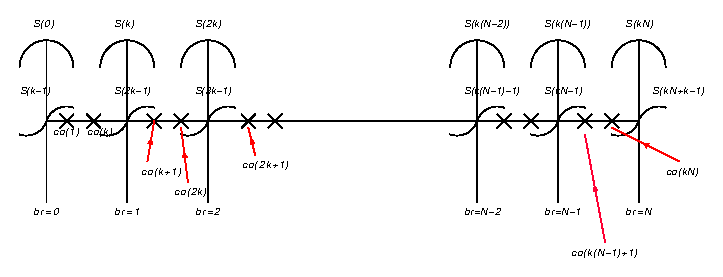
\includegraphics{splinemethod.eps}
%\caption{spline method explanation}
%\label{fig:spline}
%\end{figure}


미분 방정식을 푸는 방법에는 여러가지가 있지만, 3-body 이상의
partial differential equation의 경우에는 spline function을 
이용하여 eq.을 discrete matrix linear algebra equation으로 
바꾸는 것이 편리하다.

기본적으로 interpolation을 통해 함수를 basis spline function 의 linear combination으로 나타내고,
풀고자하는 식을 spline coefficient 에 대한 식으로 바꾸어 준다. 
이를 위해서 필요한 것은 (1) 주어진 문제를 spline coefficient에 대한 식으로 바꾸기.
(2) 얻어진 spline coefficient를 이용하여 임의의 점에서 함수의 값 구하기. 
또는 주어진 함수의 값들로부터 spline coefficient 구하기 가 가능해야한다. 


\subsection{Cubic Hermite spline}
\begin{figure}[h!]
\begin{center}
%\mbox{\epsfxsize=6cm\epsffile{CubicHermite.eps}}
\includegraphics[height=60mm]{CubicHermite1.png}
\end{center}
\caption{Cubic Hermite functions.}
\label{fig:spline}
\end{figure}
Spline method uses order $k$ spline functions for
interpolation of function and discretization
of equation. This is better for 
interpolate function and its derivative, thus
suitable for differential equation.
Cubic Hermite spline interpolation in interval $(x_i,x_{i+1})$
can be written for function $y=f(x)$, 
\bea
f(x)=h_{00}(t)y_i+h_{10}(t)(x_{i+1}-x_i)m_i
    +h_{01}(t)y_{i+1}+h_{11}(t)(x_{i+1}-x_i) m_{i+1} 
\eea 
where, $t=(x-x_i)/(x_{i+1}-x_i)$ (즉, t는 $x_i(t=0)$와 $x_{i+1}(t=1)$을 잇는
parameter) and 
$m_i$ is a value of tangent function at point $x_i$.
Basis functions are given as
\begin{equation}
\begin{array}{l|l|l}
           &\mbox{ expanded}& \mbox{factorized} \\
           \hline 
 h_{00}(t)=S_{2i}(t) & 2t^3-3t^2+1    & (1+2t)(1-t)^2     \\
 h_{10}(t)=S_{2i+1}(t) & t^3-2t^2+t     & t(1-t)^2          \\
 h_{01}(t)=S_{2i+2}(t) & -2t^3+3t^2     & t^2(3-2t)         \\
 h_{11}(t)=S_{2i+3}(t) & t^3-t^2        & t^2(t-1)\\
\end{array} 
\end{equation}
여기서, tangent function $m$ is not unique.
Let us choose here $m_i=\frac{d}{dx}f({x=x_i})$
or numerically equivalent choices
\bea
m_i=\frac{y_{i+1}-y_{i-1}}{x_{i+1}-x_{i-1}},\mbox{ or }
m_i=\frac{y_{i+1}-y_i}{2(x_{i+1}-x_i)}
   +\frac{y_{i}-y_{i-1}}{2(x_{i}-x_{i-1})}.
\eea
따라서, $x_i<x<x_{i+1}$ 에서의 함수값을 interpolate하기 위해서는,
$y_{i-1},y_{i},y_{i+1},y_{i+2}$ 또는,
$y_{i},y'_i,y_{i+1},y'_{i+1}$ 의 4개의 함수 값이 필요하다. 

In a form of matrix, for $x_i<x<x_{i+1}$ and $t=(x-x_i)/(x_{i+1}-x_i)$
(허? 이 식 맞나?)
\bea 
f(t)&=&\left( \begin{array}{cccc} t^3 & t^2 & t & 1\end{array} \right)
     \left( \begin{array}{cccc} 2 & 1 & -2 & 1 \\
                                -3 & -2  & 3 & -1 \\
                                0 & 1 & 0 & 0 \\
                                1 & 0 & 0 & 0 \end{array} \right)  
     \left(\begin{array}{c} y_i \\ y'_i \\ y_{i+1} \\ y'_{i+1} \end{array}\right) \no 
    &=&\left[ \begin{array}{c} 2 t^3-3t^2+1 \\
                               t^3-2t^2+t \\
                               -2 t^3 +3t^2 \\
                               t^3-t^2 
              \end{array} \right]^T  
         \left(\begin{array}{c} y_i \\ y'_i \\ y_{i+1} \\ y'_{i+1} \end{array}\right)                             
\eea 

 We may rename basis functions as $S_{n}(x)$.
so that spline function $S_{2i}(x_i)=1$ and 
$S'_{2i+1}(x_i)=1$.
그러면, $x_i<x<x_{i+1}$ 에서
\bea
f(x)=C_{2i} S_{2i}(x)+C_{2i+1}S_{2i+1}(x)+C_{2i+2}S_{2i+2}(x)
    +C_{2i+3}S_{2i+3}(x)
\eea
으로 interpolation 하게 된다. 이 때, $S_{2i}(x)$ and $S_{2i+1}(x)$
는 $x_{i-1}<x<x_{i+1}$ 사이에서 정의되는 함수이다.(단, 경계에서는
$S_{0,1}(x)$는 $x_0<x<x_1$에서 정의된 함수.)이고, spline coefficient
$C_{2i}=y_i$ and $C_{2i+1}=y'_i$ 로 결정된다.

즉,
\bea 
f(x_i)=C_{2i},\quad f'(x_i)=C_{2i+1},\quad 
f(x_{i+1})=C_{2i+2},\quad f'(x_{i+1})=C_{2i+3}.
\eea 
문제는 보통 함수의 미분값이 알려져 있지 않다는 것. 

Thus, $S_{2i}(x)$ and $S_{2i+1}(x)$ is defined as
\begin{equation}
\begin{array}{c|c|c|c}
      &  x_{i-1}<x<x_i & x_i<x<x_{i+1} & \mbox{C}\\ \hline
  t   & \frac{x-x_{i-1}}{x_i-x_{i-1}},\ t=(0,1) 
      & \frac{x-x_i}{x_{i+1}-x_i},\ t=(0,1) 
      & \\
  S_{2i}(x) & t^2(3-2t)    & (1-t)^2(1+2t) & C_{2i}=y_i\\
  S_{2i+1}(x) & -(x_i-x_{i-1})t^2(1-t) & (x_{i+1}-x_i)t(1-t)^2 
              & C_{2i+1}=y'_i\\
\end{array}
\end{equation}
Thus, given list of break points and values of $y_i$ and $y'_i$
at break points determines all spline functions and 
its coefficients.

When the range of points are not the same, 
we need additional boundary conditions
to convert one basis to the other in whole range.
(Interpolation near the boundary would involve extrapolation 
without boundary condition.) 



\subsection{Discretizing Differential equation}
미분 방정식
$$\hat{L} F(r)=0 $$ 을 푸는 경우, $0\le r\le r_N$ can be interpolated as
\bea
F(r)\simeq \sum_{j=0}^{k(N+1)-1} C_j S_j(r).
\eea
하지만, 동시에 미분 방정식을
matrix로 바꾸기 위해서는 $r$ 을 mesh points로 나누어야 한다.
이 경우 mesh points를 각 break point 사이의 interval 에 대한
legendre quadrature로 잡는 것이 편리하다.

 spline function 의 index는
전체 구간을 $x_0,..,x_N$ 의 break point로 나누었을 때,
각 break point마다 k 개의 spline function이 배당되는
식으로 정한다. 그리고, 각 interval,$[x_i,x_{i+1}]$ , 
에서 non-zero인 spline function은 break point
$x_i$와 $x_{i+1}$ 에 해당하는 spline function뿐이다.  
그러면, differential equation은
\bea
\sum_{j=0}^{k(N+1)-1} C_j [\hat{L} S_j(r)]=0
\eea
으로 바뀌고, 우리는 total $k(N+1)$개의 unknown coefficient
$C_j$를 구해야한다. 이 때, collocation point $col_1,..col_{kN}$ 
point에서의 식들을 independent 하게 취급하여, $KN$ 개의
식을 얻을 수 있다. 나머지, k 개의 조건은 boundary 
condition으로부터 얻을 수 있다.
예를 들어, $k=2$ 인 경우 boundary condition에 의해서,
$C_0,C_1,...,C_{2N},C_{2N+1}$ 중에
\bea
& &F(r=0)=0=C_0\no
& &F(r=r_N)=C_{2N} 
\eea
으로 $C_0$와 $C_{2N}$가 미리 결정된다. 
따라서, k-개의 boundary condition 을 포함하여, 
\bea
\sum_{j=0}^{k(N+1)-1} C_j [\hat{L} S_j(r_i)]=0,\mbox{
 $i$ 는 $1,2,\dots,k(N+1)$}
\eea
의 식이 얻어진다. 그리고, $[\hat{L} S_j(r_i)]\to [A]_{i,j}$
로 matrix로 나타내면,
\bea
[A]c=0
\eea
의 linear algebra problem 으로 바뀐다. 여기서,
$[A]$ 와 $c$ 는 dimension 이 $k(N+1)$ 으로 쓰거나,
이미 $k$ 개의 $C$ 가 결정되어 있으므로, $kN$ 만의 
식으로 쓸 수 있다. 단, $kN$ 개 coefficient 만의
식을 쓸 경우, bound state라면, 나머지 모든 coefficient가 
zero 이므로, 새로운 term 이 나타나지 않지만,
scattering state의 경우에는 boundary condition에 의해서,
\bea
[A]c=b
\eea
와 같이 boundary 에서의 coefficient 에 비례하는 
term 이 나타나게 된다.
이 때, 
\bea
[b]_i=-\sum_{j=kN+1}^{k(N+1)-1} C_j[\hat{L} S_j(r_i)],
\mbox{ i 는 $kN+1,\dots,k(N+1)$}
\eea
이고, $C_j$는 boundary 즉 last break point 에서의 
$F(r_N)$ 및 그 derivative 에 의해서,
\bea
C_{kN}=F(r=r_N),\quad C_{kN+1}=F'(r=r_N),\dots
\eea
결정된다. 

실제 계산에서는 boundary condition 을 $r=0$ 과
$r=r_{max}$ 에서의 값으로 주는 것이 보통이다. 
이런경우에는 
식을 어떻게 써야할까? 
\bea
F(r)\simeq \sum_{j=0}^{k(N+1)-1}C_j S_j(r)
     =\sum_{j=1}^{kN} C_j S_j(r)
     +\sum_{j=kN+1}^{kN+k-1} C_j S_j(r)    
\eea
이고, 특히 $k=2$인 경우는, $C_0=0$인 경우 $(F(0)=0)$
\bea
F(r)&=&\sum_{j=1}^{2N-1} C_j S_j(r)
       +C_{2N}S_{2N}(r)+C_{2N+1}S_{2N+1}(r)   
\eea
로 쓸 수 있고, 이 중 $C_{2N}$은 boundary condition
에 의해서, $C_{2N}=F(r=r_N)$ 으로 이미 결정되어 있다.
따라서, 마지막 2개의 spline coefficient 및
spline function의 이름을 바꾸어, 
\bea
F(r)=\sum_{j=1}^{kN} \tilde{C}_j \tilde{S}_j(r)
       +F(r_N)\tilde{S}_{2N+1}(r) ,   
\eea
where
\bea 
C_{2N}S_{2N}(x)=\tilde{C}_{2N+1}\tilde{S}_{2N+1}(x),\quad
C_{2N+1}S_{2N+1}(x)=\tilde{C}_{2N}\tilde{S}_{2N}(x),
\eea 

형식으로 쓸 수 있다. 단, 이경우, 마지막 
spline function
$\tilde{S}_{2N}(r), \tilde{S}_{2N+1}(r)$ 은 
실제로는 $S_{2N+1}(r), S_{2N}(r)$ 이고,
$\tilde{C}_{2N}$ 은 $F'(r_N)$에 해당한다는 점에 주의할 것. 만약, bound state
였다면, 위 식에서 마지막, $\tilde{S}_{2N+1}(r)$의 coefficient를 zero
로 둘 수 있게 된다. 따라서, $C_{1\dots 2N}$ 의 unknown
coefficients를 구하는 문제로 바뀐다.
따라서, collocation points $r_1,\dots r_{2N}$ 에 대한 식은
\bea
\hat{L}F(r_i)=\sum_{j=1}^{2N}[\hat{L}\tilde{S}_j(r_i)]C_j
              +F(r_N)\hat{L}\tilde{S}_{2N+1}(r_i)=0
\to \sum_j [A]_{ij}[C]_j +[B]_i=0  
\eea
으로 쓸 수 있게 된다. 2차 미방의 경우, we can have two solutions,
$[C^{(1)}]_j$ and $[C^{(2)}]_j$ 를 2개의 boundary condition
으로 부터 구할 수 있고, normalization factor는 boundary condition과의
matching 으로 구할 수 있다.

하지만, scattering problem 에서는 asymptotic wave function 
의  phase shift/K-matrix 가
미리 알려져 있지 않기 때문에 $F(r_N)$ 을 미리 결정해서 줄 수가 없다. 
만약 전체 미방이 homogeneous 라면, 미리, $F(r_N)=1$ 으로
scale 된 문제를 푼 다음에, K-matrix 를 나중에 구해서 다시 보정할 할 수 있을 것이다. 
\bea
\phi_{\alpha}(r)\sim \frac{[j_\alpha(kr)\delta_{\alpha\beta}
                    -K_{\alpha\beta} n_\beta(kr)]}
                    {[j_\alpha(kr_N)\delta_{\alpha\beta}
                    -K_{\alpha\beta} n_\beta(kr_N)]}
                    \to\ C_{2N}=1
\eea
$r_{match}<r_N$ 에서의 solution을 이용하여 matching 
하면 K-matrix를 결정할 수 있고, 따라서, 거꾸로 $C_{2N}=F(r_N)$ 을 다시 
보정해 줄 수 있다.     

Inhomogeneous equation의 경우에도 풀어야하는 방정식 자체는 비슷하다. 
Scattering 문제의 경우에는 $[B]_j$ 안에 inhomogeneous term 이 포함되게 된다. 
문제는 Inhomogeneous equation에서는 $F(r_N)$ 을 임의로 
scale 할 수 없을 것이라는 점이다. 
Boundary condition을 어떻게 주어야 할까? 이 경우에는 
asymptotic boundary conditiond르 이용하여 $F(r_N)$ 이 
$F'(r_N)$의 함수가 되도록 만들면, equation에서 $F(r_N)$ 을 없앨 수가 있다.  
예를 들어 asymptotic form 이 $S*g(r)$ 로 unknown $S$ 를 포함하더라도 ,
logarithmic derivative continuous condition은 
\bea 
\frac{F'(r=r_N)}{F(r=r_N)}=\frac{g'(r=r_N)}{g(r=r_N)}
\eea 
이 되어 matrix equation에서 $F(r_N)$ 대신 $F'(r_N)$을 사용할 수 있게 된다. 

\subsubsection{Converting collocation point values to spline coefficient}

한편, 주어진 collocation points value들로 부터 spline coefficient를 역으로
구하는 것은

\bea
F(r_i)=\sum_{j=0}^{2N+1} C_j S_j(r_i)
      =\sum_{j=1}^{2N} \tilde{C}_j \tilde{S}_j(r_i) 
                     +F(r_N)\tilde{S}_{2N+1}(r_i)
\eea 
로 쓸 수 있다. 따라서, matrix를
$S_{ij}=S_j(r_i)$ 로 정의하면,
\bea
C_j=\sum_{i=0}^{2N+1} [S^{-1}]_{ji} F(r_i),\mbox{ or }
\tilde{C}_j=\sum_{i=1}^{2N}[\tilde{S}^{-1}]_{ji}
                [F(r_i)-F(r_N)\tilde{S}_{2N+1}(r_i)]
\eea
로 구할 수 있다.

\subsubsection{예}
간단한 예를 들어 보자. 문제를 단순히 하기 위해서, cubic hermite polynomial (k=2)
경우이고 구간이 단순히 $x_0$ 와 $x_1$ 인 경우만 생각해보자. 이 구간에서
임의의 함수값은
\bea
f(r)\simeq C_0 S_0(r)+C_1 S_1(r)+C_2 S_2(r)+C_3 S_3(r)
\eea
으로 정해진다. boudary condition에 의해서 4 개의 coefficient 중 오직 
2개만이 unknown 이된다. 미분 방정식도
\bea
[L]f(r)=C_0 [L]S_0(r)+ C_1[L]S_1(r)+ C_2 [L]S_2(r)+ C_3 [L] S_3(r)=[B](r)
\eea
로 주어진다. 경계 조간에 따라서, 풀어야하는 선형방정식이 달라지게 된다.
예를 들어 $f(x_0)=0$, $f(x_1)=0$(or $C_0=C_2=0$ 
의 2-boundary value가 주어지는 경우.
두 점 $r_1, r_2$ 에서 다음을 풀면된다.
\begin{equation}
\left(\begin{tabular}{cc} $[L]S_1(r_1)$ & $[L]S_3(r_1)$ \\
                          $[L]S_1(r_2)$ & $[L]S_3(r_2)$ \end{tabular}
\right)\left( \begin{tabular}{c} $C_1$ \\ $C_3$ \end{tabular}\right)
=\left( \begin{tabular}{c} $[B](r_1)$ \\ $[B](r_2)$ \end{tabular}\right)
\end{equation}

거꾸로 만약 함수의 collocation points 에서의 값이 주어져 있을 때,
정해진 knot 에서 정의된 spline basis function에 대한 
spline coefficient는 다음과 같이 구할 수 있다.
\bea
f(r_1)&=& C_1 S_1(r_1)+ C_3 S_3(r_1),\no
f(r_2)&=& C_1 S_1(r_2)+ C_3 S_3(r_2)
\eea
because $C_0=0$ and $C_2=0$ is already known. (즉, boundary condition을 이용해야한다.)
또는 collocation point들을 새로운 knot으로 생각하여, 새로 basis function을 만들어
interpolation하여 원래 knot에서의 함수값과 미분값을 계산하도록 할 수도 있다. 

\subsection{Explicit form of matrix equation}
Differential equation we would like to solve is
\bea 
\left[ -\frac{1}{2\mu}\frac{d^2}{dx^2}+\frac{1}{2\mu}\frac{l'(l'+1)}{x^2}-E\right] 
u_{l' l}(x)+\sum_{\beta} x V_{l'\beta}(x) \frac{u_{\beta l}(x)}{x} =0
\eea 
With using last term exchanged spline function $\tilde{S}_j(x)$,
we will interpolate
\bea 
u_{\alpha\beta}(x)&=&\sum_{j=0}^{2N+1}\tilde{C}_{\alpha,j}^{\beta} \tilde{S}_j(x) \no 
                  &=&\sum_{j=1}^{2N} \tilde{C}_{\alpha,j}^{\beta} \tilde{S}_j(x)
                  +\tilde{C}_{\alpha,0}^{\beta} \tilde{S}_0(x)
                  +\tilde{C}_{\alpha,2N+1}^{\beta} \tilde{S}_{2N+1}(x)
\eea 
Then, above equation becomes
\bea 
& &\sum_{\beta=1}^{N_{s}}\sum_{j=0}^{2N+1} 
\left[-\frac{1}{2\mu}\frac{d^2}{dx^2}\tilde{S}_j(x)\delta_{l',\beta}
     +\frac{1}{2\mu}\frac{l'(l'+1)}{x^2}\tilde{S}_j(x)\delta_{l',\beta}-E\tilde{S}_j(x)\delta_{l',\beta}
     \right]
     \tilde{C}_{\beta,j}^{l} \no 
& &+\sum_{\beta=1}^{N_{s}}\sum_{j=0}^{2N+1}
 \left[x V_{l'\beta}\frac{\tilde{S}_j(x)}{x} \right]\tilde{C}_{\beta,j}^{l} =0
\eea 
By choosing $x_i$ points, $i\in[1,2N]$, 
we can have $2N$ number of equations.
Let us define vectors and matrices as
\bea 
[\tilde{C}^l]_{n}&\equiv& \tilde{C}^l_{\beta,j} ,
\eea
\bea 
[\Delta]_{n'n}&\equiv& 
         -\frac{1}{2\mu}\frac{d^2}{dx^2}\tilde{S}_j(x_i)\delta_{l',\beta}
              +\frac{1}{2\mu}\frac{l'(l'+1)}{x_i^2}\tilde{S}_j(x_i)\delta_{l',\beta},   
\eea 
\bea 
[B]_{n'n}&\equiv& \tilde{S}_j(x_i) \delta_{l'\beta}, 
\eea 
\bea 
[V]_{n'n}&\equiv& x_i V_{l'\beta}(x_i)\frac{\tilde{S}_j(x_i)}{x_i}, 
\eea 
with
\bea 
n'\equiv(l',i) \mbox{ and }  n\equiv(\beta,j),
\eea 
Then, above equation can be rewritten as matrix equation,
\bea 
\sum_{\beta=1}^{N_{s}}\sum_{j=0}^{2N+1}[\Delta -E B +V]_{n'n}[\tilde{C}^l]_n=0.
\eea 
Note that number of index is different between $n'$ and $n$. 
We have to use boundary conditions to make the above equation to be 
square. 

Let us denote $n_0\equiv(\beta,0)$ and $n_f\equiv(\beta,2N+1)$ and separate
\bea 
\sum_{\beta=1}^{N_{s}}\sum_{j=1}^{2N}[\Delta -E B +V]_{n'n}[\tilde{C}^l]_n
+\sum_{\beta=1}^{N_{s}}[\Delta -E B +V]_{n'n_0}[\tilde{C}^l]_{n_0}
+\sum_{\beta=1}^{N_{s}}[\Delta -E B +V]_{n'n_f}[\tilde{C}^l]_{n_f}
=0.
\eea 
For bound state problem, we can use boundary condition as
\bea 
[\tilde{C}^l]_{n_0}=0,\quad [\tilde{C}^l]_{n_f}=0, \mbox{ for all }\beta. 
\eea  
and the matrix equation becomes eigenvalue problem
\bea 
{\sum_{n}}'[\Delta+V]_{n'n}[\tilde{C}^l]_n=E{\sum_{n}}'[B]_{n'n}[\tilde{C}^l]_n,
\quad \mbox{ with } {\sum_{n}}'\equiv \sum_{\beta=1}^{N_s}\sum_{j=1}^{2N}.
\eea 

For the scattering case, we have to use asymptotic form of wave function as boundary 
condition,
\bea 
[\tilde{C}^l]_{n_0}=0,\quad 
[\tilde{C}^l]_{n_f}= u_{\beta l}(r=r_N)
                   =\frac{1}{2}r[\delta_{\beta l} h_{\beta}^{(-)}(kr)
                                 +S_{\beta l} h_{\beta}^{(+)}(kr)]   
.
\eea 
and the matrix equation becomes
\bea 
{\sum_{n}}'[\Delta+V-E B]_{n'n}[\tilde{C}^l]_{n}
=[ G^l ]_{n'},
\quad [G^l]_{n'}\equiv -\sum_{\beta=1}^{N_{s}}[\Delta -E B +V]_{n'n_f}[\tilde{C}^l]_{n_f}
\eea 

But, in fact, asymptotic form of $u_{\beta l}$ contains unknown 
complex S-matrix. Because of homogeneous form of the equation, 
we can change normalization of solution. 
However, still it does not completely fix boundary condition if it is a coupled equation.
How should we solve the problem? 

{\bf Possible answer?:} M원 N차 연립 미분 방정식의 general solution은 
M*N 개의 independent boundary condition을 통해 얻은 M*N개 
solution들의 선형 결합으로 표현된다? 만약 이 주장이 옳다면, 위 문제에서 
regular solution 에 한정해서, $[\tilde{C}^l]_{nf}=\delta_{\beta l}$ 
로 모든 $l=1..N_s$ 개의 different boundary condition으로 부터  
$N_s$ 개의 solution을 구한다음 이것들이 어떻게 결합하여 원하는 boundary condition을 줄 수 있는지
구하면 된다. So, we will let 
\bea 
[G^l]_{n'}\equiv -\sum_{\beta=1}^{N_{s}}[\Delta -E B +V]_{n'n_f} \delta_{\l \beta}
             = -[\Delta -E B +V]_{n'(l,2N+1)}
\eea 
And solve for different $l$'s and get $N_s$ different solutions. Then, 
recombine them to obtain asymptotic boundary condition and fix the S-matrix. 

Suppose we obtained $[\tilde{C}^{l=1..N_s}]_{i=1..2N}$. Then how can we find the
correct normalization and S, K matrix?


\subsection{Special case: perturbation}
In case of inhomogeneous PV equation, 
\bea 
\left[ -\frac{1}{2\mu}\frac{d^2}{dx^2}+\frac{1}{2\mu}\frac{l'(l'+1)}{x^2}-E\right] 
u^{PV}_{l' l}(x)+\sum_{\beta} x V^{PC}_{l'\beta}(x) \frac{u^{PV}_{\beta l}(x)}{x}
+\sum_{\beta} x V^{PV}_{l'\beta}(x) \frac{u^{PC}_{\beta l}(x)}{x}
 =0,
\eea
we can transform the equation into matrix equation,
\bea 
& &\sum_{\beta=1}^{N_{s}}\sum_{j=1}^{2N}[\Delta -E B +V^{PC}]_{n'n}[\tilde{C}^{PV,l}]_n \no 
& &+\sum_{\beta=1}^{N_{s}}[\Delta -E B +V^{PC}]_{n'n_0}[\tilde{C}^{PV,l}]_{n_0}
+\sum_{\beta=1}^{N_{s}}[\Delta -E B +V^{PC}]_{n'n_f}[\tilde{C}^{PV,l}]_{n_f} \no 
& &+\sum_{\beta=1}^{N_s}\sum_{j=0}^{2N+1}[V^{PV}]_{n'n}[\tilde{C}^{PC,l}]_{n} 
=0.
\eea  
Suppose we already solved the parity conserving wave function, 
the last term is already known and we can write as
\bea 
[K^l]_{n'} \equiv -\sum_{\beta=1}^{N_s} x_i V^{PV}_{l'\beta}(x_i) \frac{u^{PC}_{\beta l}(x_i)}{x_i}
\eea 

However, the boundary condition for $u^{PV}$ as   
\bea 
[\tilde{C}^{PV,l}]_{n_0}=0, \quad [\tilde{C}^{PV,l}]_{n_f}=u^{PV}_{\beta l}(r=r_N),
\eea 
is not directly applicable because it contains unknown scattering matrix
and also cannot be arbitrarily scaled,
\bea 
u^{PV}_{\beta l}(r)=\frac{1}{2}S^{PV}_{\beta l} h^{(+)}_{\beta}(kr),
\eea 
where there is no $\delta_{\beta l}$ because $\beta\neq l$ for PV transition.
But we can use logarithmic derivative continuous condition,
\bea 
\frac{1}{u^{PV}_{\beta l}(r)}\frac{d u^{PV}_{\beta l}(r)}{dr}
=\frac{1}{ h^{(+)}_{\beta}(kr)}
 \frac{d h^{(+)}_{\beta}(kr)}{dr}
\eea 
Thus replace
\bea 
u^{PV}_{\beta l}(r=r_N)=\frac{h^{(+)}_{\beta}(kr_N)  }{ \frac{d }{dr}h^{(+)}_{\beta}(kr_N)} 
                       \frac{d u^{PV}_{\beta l}(r_N)}{dr}
                       =\frac{h^{(+)}_{\beta}(kr_N)  }{ \frac{d }{dr}h^{(+)}_{\beta}(kr_N)}
                       \tilde{C^l}_{\beta,2N} =\tilde{C^l}_{\beta,2N+1} 
\eea 
and change 
\bea 
& &\sum_{\beta=1}^{N_{s}}[\Delta -E B +V]_{n'n_f}[\tilde{C}^{PV,l}]_{n_f} \no 
&+&\sum_{\beta=1}^{N_s}\sum_{j=1}^{2N} \left[ \delta_{j,2N}
   [\Delta-E B+V^{PC}]_{n',n_f} 
   \left(\frac{h^{(+)}_{\beta}(kr_N)  }{ \frac{d }{dr}h^{(+)}_{\beta}(kr_N)}\right) 
   \right] 
   [\tilde{C}^{PV,l}]_{n} \no 
&\equiv& {\sum_{n}}'[X]_{n'n}[\tilde{C}^{PV,l}]_{n}   
\eea 
And finally the equation becomes
\bea 
{\sum_n}' [\Delta+V^{PC}- E B+X]_{n'n}[\tilde{C}^{PV,l}]_{n}=[K^l]_{n'}
\eea 
After obtaining $[\tilde{C}^{PV,l}]_{n}$, we can obtain 
\bea 
S^{PV}_{\beta l}=\frac{ 2 \tilde{C}^{PV,l}_{\beta,2N} }{ \frac{d }{dr}h^{(+)}_{\beta}(kr_N)}
\eea 

One subtle point in above expression is that $\beta$ must contain 
both parity even and parity odd states. For example we choose
$l'=1$ and $l=0$, $\sum_{n}$ in the above matrix equation 
must be parity odd states but $\sum_{\beta}$ in $[K]$ must be parity even states.
Also, we have to solve the matrix equation for complex coefficients, unlike Parity conserving case.

\subsection{Practical implementation }
먼저, potential 이 real인 경우, complex normalization factor를 밖으로 빼어내서, 
우리는 언제나 real-valued solution을 얻을 수 있다. scattering state의 경우에는 complex 
normalization factor 를 
\bea
\label{spline:interp} 
R_{\alpha',\alpha}(x)=\sum_{\beta} \hat{R}_{\alpha',\beta}(x)[\frac{1+\hat{S}}{2}]_{\beta\alpha},
\no 
\hat{R}_{\alpha',\beta}(x)\to \delta_{\alpha',\beta} j_{L'}(kx)
                             -\hat{K}_{\alpha'\beta} n_{L'}(kx) 
\eea 
로 빼낼 수 있고, normalization 은 
\bea 
\label{spline:SK}
[\frac{1+\hat{S}}{2}]_{\beta\alpha}=[(1-i\hat{K})^{-1}]_{\beta,\alpha}
\eea 
을 이용해  K-matrix로 나타낼 수 있다. 

한편, 실제 계산에서 우리가 다루는 것은 spline coefficient 에 관한 equation이다. 따라서, 
\bea 
\hat{R}_{\alpha,\beta}(x)=\sum_{j=1}^{2N_x} \tilde{C}^{\beta}_{\alpha,j} \tilde{S}_j(x)
                           +\tilde{C}^{\beta}_{\alpha,2N_x+1} \tilde{S}_{2N_x+1}(x)
\eea 
이것은 위의 K-matrix 와 다음 식을 만족해야 한다. 
\bea 
\tilde{C}^{\beta}_{\alpha,2N+1}&=& \hat{R}_{\alpha,\beta}(x_N)
                                 =\delta_{\alpha,\beta} j_{\alpha}(kx_N)
                                 -\hat{K}_{\alpha\beta} n_{\alpha}(kx_N),\no  
\tilde{C}^{\beta}_{\alpha,2N}&=& \hat{R}'_{\alpha,\beta}(x_N)
                                 =\delta_{\alpha,\beta} j'_{\alpha}(kx_N)
                                 -\hat{K}_{\alpha\beta} n'_{\alpha}(kx_N).
\eea 
따라서, 
\bea 
\label{spline:last}
K_{\alpha\beta}&=&\left[
    \frac{\delta_{\alpha\beta}j'_\alpha(kx_N)-\tilde{C}^{\beta}_{\alpha,2N}}
    {n'_\alpha(kx_N)}      \right],
\no 
\tilde{C}^{\beta}_{\alpha,2N+1}&=&
 \left[\delta_{\alpha,\beta} j_{\alpha}(kx_N)
       -\delta_{\alpha\beta}\frac{n_\alpha(kx_N)}{n'_\alpha(kx_N)} j'_{\alpha}(kx_N)\right] 
   +\tilde{C}^\beta_{\alpha,2N} \frac{n_\alpha(kx_N)}{n'_\alpha(kx_N)}    
\eea 
으로 $\tilde{C}^\alpha_{\beta,(2N)}$ 값으로 모두 나타낼 수 있다. 따라서, linear algebra 문제를 
푸는데 두 가지 접근을 생각해 볼 수 있다. eq.(\ref{spline:interp})에 eq.(\ref{spline:last})를 
대입하여, 식을 $\tilde{C}^\alpha_{\beta,1:2N}$ 에 대한 inhomogeneous equation으로 만들어서 
풀면, normalization condition까지 고려한 결과 $\tilde{C}^\alpha_{\beta,1:2N}$를 한 번에 
얻게 된다. 한 편, 위와 같이 푸는 대신, 
$\tilde{C}^\beta_{\alpha,2N+1}=\delta_{\alpha,\beta}$의 boundary condition 을 주어 
모든 $\beta$ 에 대한 solution을 얻은 뒤 다시 normalization을 restore 해주는 방법이다. 
이렇게 구해진 spline coefficient solution을 $D^\beta_{\alpha,j}$ 라고 하자. 
즉, 우리는 
\bea 
\label{spline:CD}
\tilde{C}^\beta_{\alpha,j}=\sum_{\gamma} M_{\alpha\gamma}\tilde{D}^\gamma_{\beta,j}
,\quad 
\tilde{D}^\beta_{\alpha,2N+1}= \delta_{\alpha,\beta},
\quad 
\eea 
인 solutions $\tilde{D}^\beta_{\alpha,j}$ 를 얻었다고 하자. 
Conversion factor or Normalization factor $M_{\alpha\gamma}$ can be obtained from
the comparison with eq.(\ref{spline:last}), $M_{\alpha\beta}=\tilde{C}^\beta_{\alpha,2N+1}$.
하지만, $\tilde{C}$ 는 미리 알려진 것이 아니므로, M 을 D로 나타내어 주면,\footnote{
It is possible that the number of interested coupled channels is less than 
the number of internal partial wave states. In that case, matrix M can be non-square.
But, nonetheless the equation can be solved.
$ [M(N_s\times N_{ch}) [D(N_{ch}\times N_s)]=[N_s\times N_s]$, which can be 
changed into the form of $Ax=b$ by transpose the equation. 

}
\bea 
\label{spline:M}
\sum_{\gamma} M_{\alpha\gamma}\left[\tilde{D}^\gamma_{\beta,2N+1}-
                        \tilde{D}^\gamma_{\beta,2N}\frac{n_\alpha(kx_N)}{n'_\alpha(kx_N)}\right] 
 =\left[\delta_{\alpha,\beta} j_{\alpha}(kx_N)
        -\delta_{\alpha\beta}\frac{n_\alpha(kx_N)}{n'_\alpha(kx_N)} j'_{\alpha}(kx_N)\right]  
\eea  
으로부터 , $M_{\alpha\gamma}$를 구할 수 있다. Note here $\gamma=1:N_{ch}$ but $\alpha,\beta=1:N_s$.

In summary, the steps we need to takes are
\begin{enumerate}
\item Solve and obtain solutions for coupled channels
      $\tilde{D}^\gamma_{\alpha, j}$ for $j=1:2N$ 
      with boundary conditions
      $\tilde{D}^\beta_{\alpha,2N+1}= \delta_{\alpha,\beta}$. 

\item Obtain conversion matrix $M$ from eq.(\ref{spline:M} ).

\item Obtain $\tilde{C}$ from eq. (\ref{spline:CD}).

\item Obtain $K$-matrix and last spline coefficients from eq.(\ref{spline:last})

\item Obtain complex normalization and S-matrix from eq.(\ref{spline:SK})

\item Finally, full wave function can be obtained 
      by multiplying complex normlaization to real valued solutions. 
 
\end{enumerate}

Until now we used notation $n=(\beta,j)$ 
to represent both partial wave quantum number and
spatial coordinate ot spline index. In practical implementation, it would be better
to introduce 1-D index
\bea 
k=(\beta-1)*(k N_x)+j, \quad \beta=1\dots N_s,\quad j=1\dots k N_x,
\eea 
so that the wave function $F_{\alpha,i}(x)$ can be written as 1-D array
$F_i(k=1\dots N_s k N_x)$ with only external index for initial channel $i$.
If we have coupled channels, we would want match 
\bea 
F^{full}_i(1:N_s k N_x)=\sum_j N_{ij} F^{num}_{j}(1:N_s K N_x),
\eea   
where, $F^{full}_i(1:N_s k N_x)$ is a full complex wave function with correct 
normalization and asymptotic form in channel $i$,
$F^{num}_{j}(1:N_s K N_x)$ is a numerical solution with boundary 
condition of $[\tilde{C}^j]_{nf}=\delta_{\beta j}$ and $N_{ij}$
is a complex normalization matrix to match $F^{full}_i$. 


\subsection{Lanczos method: iteration method}
앞에서 3-body 문제를 spline method를 이용하여
linear algebra 문제로 바꾸는 것을 살펴보았다.
여기서는 linear algebra problem 특히 bound state의 경우에
large matrix에 대해 효율적으로 푸는 방법을 살펴보자. 이것은 다음 3-body 노트에서 이야기하자.


\newpage
\section{T-amplitude with two different potential
(Alternate derivation of DWBA)
}
Let us call there are two potentials 
$\hat{V}=\hat{V}_Y+\hat{C}$.
In operator form, the T matrix will be written as
\bea
\hat{T}=\hat{V}+\hat{V}\hat{G}_0\hat{T}
       =\hat{V}+\hat{V}\hat{G}\hat{V} 
\eea
We introduce Green's functions and $\hat{T}_Y$ as
\bea
& &\hat{G}^{(+)}=\frac{1}{E-\hat{H}_0-\hat{V}+i\epsilon},\quad
\hat{G}^{(+)}_0=\frac{1}{E-\hat{H}_0+i\epsilon},\quad
\hat{G}^{(+)}_Y=\frac{1}{E-\hat{H}_0-\hat{V}_Y+i\epsilon},\no
& &\hat{T}_Y=\hat{V}_Y+\hat{V}_Y\hat{G}_0\hat{T}_Y
            =\hat{V}_Y+\hat{V}_Y\hat{G}_Y\hat{V}_Y  
\eea
From the relation between Green's functions, we get formal relations
\footnote{In general, we can use matrix relations 
\bea
B(1-AB)^{-1}=(1-BA)^{-1}B, \quad
(1-A)^{-1}=1+A(1-A)^{-1},\quad
A(1-A)^{-1}=(1-A)^{-1}A
\eea
}
\bea
\hat{G}^{-1}&=&\hat{G}_Y^{-1}-\hat{C},\no
\hat{G}&=&(\hat{G}_Y-\hat{C})^{-1}
        =(1-\hat{G}_Y\hat{C})^{-1}\hat{G}_Y
        =\hat{G}_Y(1-\hat{C}\hat{G}_Y)^{-1},\no
\hat{C}\hat{G}&=& (1-\hat{C}\hat{G}_Y)^{-1}-1
      =(1-\hat{C}\hat{G}_Y)^{-1}\hat{C}\hat{G}_Y.   
\eea
Then, 
\bea
\hat{T}&=&(\hat{V}_Y+\hat{C})
          +(\hat{V}_Y+\hat{C})\hat{G}(\hat{V}_Y+\hat{C})\no
       &=&\hat{V}_Y+\hat{C}
          +\hat{V}_Y\hat{G}\hat{V}_Y
          +\hat{C}\hat{G}\hat{V}_Y
          +\hat{V}_Y\hat{G}\hat{C}
          +\hat{C}\hat{G}\hat{C}
\eea
we can replace
\bea
\hat{V}_Y\hat{G}\hat{V}_Y
&=&\hat{V}_Y\hat{G}_Y(1-\hat{C}\hat{G}_Y)^{-1} \hat{V}_Y
 =\hat{V}_Y\hat{G}_Y[1+\hat{C}\hat{G}_Y(1-\hat{C}\hat{G}_Y)^{-1}]\hat{V}_Y
 \no
 &=&\hat{V}_Y\hat{G}_Y\hat{V}_Y
    +\hat{V}_Y\hat{G}_Y(1-\hat{C}\hat{G}_Y)^{-1}\hat{C}\hat{G}_Y\hat{V}_Y,\no
\hat{C}\hat{G}\hat{C}
     &=&   (1-\hat{C}\hat{G}_Y)^{-1}\hat{C}-\hat{C},\no 
\hat{C}\hat{G}\hat{V}_Y
 &=&(1-\hat{C}\hat{G}_Y)^{-1}\hat{C}\hat{G}_Y\hat{V}_Y,\no
\hat{V}_Y\hat{G}\hat{C}
     &=&\hat{V}_Y\hat{G}_Y(1-\hat{C}\hat{G}_Y)^{-1}\hat{C}
\eea
Thus, we get
\bea
\hat{T}=\hat{T}_Y+
(1+\hat{V}_Y\hat{G}_Y)(1-\hat{C}\hat{G}_Y)^{-1}\hat{C}
(1+\hat{G}_Y\hat{V}_Y)
\eea
We define $|\chi_\vp\ra$ such that $|\chi_\vp\ra$
is a solution of Schrodinger equation for $\hat{V}_Y$:
\bea
|\chi_\vp\ra^{(\pm)}&\equiv& (1+\hat{G}^{(\pm)}_Y\hat{V}_Y)|\vp\ra,\no
\hat{G}_Y(E_p)^{-1}|\chi_\vp\ra
&=&(E_p-\hat{H}_0-\hat{V}_Y)|\chi_\vp\ra
=(\hat{G}_Y^{-1}(E_p)+\hat{V}_Y)|\vp\ra=(E_p-\hat{H}_0)|\vp\ra=0
\eea
Thus,
\bea
\la \vp'|\hat{T}(E)|\vp\ra
=\la \vp'|\hat{T}_Y(E)|\vp\ra
 +{}^{(-)}\la \chi_{\vp'}|(1-\hat{C}\hat{G}_Y(E))^{-1}\hat{C}
  |\chi_{\vp}\ra^{(+)}
\eea
where $E$ is not neccessarily $E_p$ or $E_{p'}$ when they are not on-shell.
If $\hat{C}$ is perturbative case, we may approximate
$(1-\hat{C}\hat{G}_Y)^{-1}\simeq 1$, and we get 
DWBA approximation. Above equation corresponds to the equation (4.5) in {\bf D.B.Kaplan etal., NPB478(1996)629.}

We may express rewrite the operators in terms of $\hat{G}_0$ and $\hat{T}_Y$ from relation,
\bea
\hat{T}_Y&=&\hat{V}_Y+\hat{V}_Y\hat{G}_0\hat{T}_Y
         =\hat{V}_Y+\hat{V}_Y\hat{G}_Y\hat{V}_Y, \no 
1+\hat{G}_Y\hat{V}_Y&=& \hat{G}_Y\hat{G}^{-1},
\eea
\bea
|\chi_\vp\ra&=&(1+\hat{G}_Y\hat{V}_Y)|\vp\ra
            =(1+\hat{G}_0\hat{T}_Y)|\vp\ra,\no
(1-\hat{C}\hat{G}_Y)^{-1}\hat{C}
&=&(\hat{C}^{-1}-(1+\hat{G}_YV_Y)\hat{G}_0)^{-1}.             
\eea
This corresponds to the equation (9) of {\bf 
Long and Yang, PRC86(2012)024001.}

\section{Chiral EFT potential up to NLO}
Machleidt potential in momentum space has form,
\bea 
V(\vp',\vp)&=&V_C+\tau_1\cdot\tau_2 W_C\no
           &+&\left[V_S+\tau_1\cdot\tau_2 W_S\right]\vs_1\cdot\vs_2\no 
           &+&\left[V_{LS}+\tau_1\cdot\tau_2 W_{LS}\right]
           (-i{\bm S}\cdot(\vq\times\vk))  \no 
           &+&\left[V_T+\tau_1\cdot\tau_2 W_T\right]
           \vs_1\cdot\vq \vs_2\cdot\vq \no 
           &+& \left[V_{\sigma L}+\tau_1\cdot\tau_2 W_{\sigma L}\right]
           \vs_1\cdot(\vq\times\vk )\vs_2\cdot(\vq\times\vk ) 
\eea  
where,
\bea 
\vq=&\vp'-\vp                    & \mbox{ momentum transfer } ,\no 
\vk=&\frac{1}{2}(\vp'+\vp)       & \mbox{ average momentum } ,\no
{\bm S}=&\frac{1}{2}(\vs_1+\vs_2) & \mbox{ total spin } 
\eea 

The LO($Q^0$) chiral EFT potential involves one-pion exchange and 
contact terms. 
\bea
V_{1\pi}(\vp',\vp)=-\frac{g_A^2}{4f_\pi^2}
 \tau_1\cdot\tau_2
 \frac{\vs_1\cdot\vq \vs_2\cdot\vq}{\vq^2+m_\pi^2},
 \quad V^{(0)}=C_S+C_T\vs_1\cdot \vs_2.  
\eea
The NLO($Q^2$) chiral EFT,
\bea 
W_C&=&-\frac{L(q)}{384\pi^2 f_\pi^4}
     \left[ 4m_\pi^2(5 g_A^4-4 g_A^2-1)
            +q^2(23 g_A^4-10 g_A^2-1)
            +\frac{48 g_A^4 m_\pi^4}{\omega^2} 
     \right],\no 
V_T&=& -\frac{1}{q^2} V_S=-\frac{3 g_A^4 L(q)}{64\pi^2 f_\pi^4},   
\eea 
where,
\bea 
L(q)\equiv \frac{\omega}{q}\ln \frac{\omega+q}{2m_\pi},
\quad \omega\equiv \sqrt{4 m_\pi^2+q^2}.
\eea 
NLO contact potentials
\bea 
V^{(2)}(\vp',\vp )
&=& C_1q^2+ C_2 k^2
+(C_3 q^2+ C_4 k^2)\vs_1\cdot\vs_2 \no & & 
+C_5(-i{\bm S}\cdot (\vq\times\vk ))
+C_6(\vs_1\cdot\vq )
    (\vs_2\cdot\vq )
+C_7(\vs_1\cdot\vk )(\vs_2\cdot\vk )      
\eea 

Partial wave representation of the potential can be obtained by,
\bea 
V_{L'L}(p',p)=\int d\Omega_{\vp'}\int d\Omega_{\vp}
             Y^*_{L'}(\hat{\vp}') V(\vp',\vp)
             Y_{L}(\hat{\vp})
\eea 
Thus, if we do not include regulator, potentials in each partial wave
are 
\bea 
V^{(0)}(^1S_0)&=& 4\pi (C_S-3C_T)=\widetilde{C}_{^1S_0},\no 
V^{(0)}(^3S_1)&=& 4\pi (C_S+C_T)=\widetilde{C}_{^3S_1},\no 
V^{(2)}(^1S_0)&=& C_{1S_0} (p^{'2}+p^2)
               =4\pi (C_1+\frac{1}{4}C_2-3C_3-\frac{3}{4}C_4
                -C_6-\frac{1}{4}C_7 )(p^{'2}+p^2),\no 
V^{(2)}(^3P_0)&=& C_{^3P_0} p p'=\dots,\no 
V^{(2)}(^1P_1)&=& C_{^1P_1}pp'=\dots,\no
V^{(2)}(^3P_1)&=& C_{^3P_1}pp'=\dots,\no
V^{(2)}(^3S_1)&=& C_{^3S_1}(p^2+p^{'2})=\dots,\no
V^{(2)}(^3S_1-^3D_1)
&=& C_{^3S_1-^3D_1} p^2=\dots,\no 
V^{(2)}(^3P_2)&=& C_{^3P_2}p p'=\dots                  
\eea 

\chapter{Semi-classical scattering}
In the semiclassical approximation the dynamics of the scattering is classical, and is
described in terms of classical notions like trajectories, impact parameters, turning points,
and so on. The classical dynamical quantities enter in the calculation of the amplitude
and phase of the wave function. Typical quantal interferencε effects are preservεd in the
semiclassical approximation. 

\section{Classical scattering}
\subsection{deflection function} 
Trajectory $\vr=\vr(t)$. 

\begin{figure}
	\centering
	\includegraphics[width=0.7\linewidth]{figs/classical_scattering}
	\caption[Classical trajectory]{Classical trajectory}
	\label{fig:classicalscattering}
\end{figure}
From two equations
\bea 
E&=&\frac{\mu}{2}(\frac{dr}{dt})^2+\frac{L^2}{2\mu r^2}+V(r),\no 
L&=&\mu r^2\frac{d\phi}{dt}
\eea 
we get
\bea 
\frac{d\phi}{dr}=\frac{L}{r^2\sqrt{2\mu[E-V(r)-L^2/(2\mu r^2)]}}
\eea 
At turning point, $r=a$,
\bea 
E-V(a)-\frac{L^2}{2\mu a^2} =0.
\eea 
and 
\bea 
\phi(r)=\int_a^r dr' \frac{L}{r^{'2} \sqrt{2\mu[E-V(r')-L^2/(2\mu r^{'2})]}   }
\eea 
Deflection angle $\Theta$ from the solution at $r\to\infty$ gives deflection function 
\bea 
\Theta(b)&=&\pi-2\phi(\infty) \no 
         &=&\pi-2\int_a^\infty dr \frac{b}{r^{2} \sqrt{1-V(r)/E-b^2/r^2}}    
\eea 
Postive deflection $\Theta>0$ implies net repulsion, $\Theta<0$ imples net attraction. 

In case of classical scattering, one can tell near-side and far-side scattering. 

We can identify deflection as scattering angle for $\Theta=\theta>0$ for repulsion.
In case of attraction, $\theta=|\Theta\mod 2\pi|$. scattering cross section is
\bea 
\frac{d\sigma}{d\Omega} = \frac{b db d\phi}{|\sin\Theta d\Theta|d\phi}
                        = \frac{b}{\sin\theta|d\Theta/d b|}
\eea 

\subsubsection{Rutherford scattering}
\bea 
\Theta(b)=2\arctan(\frac{\eta}{kb}),\to b =\frac{\eta}{k}\cot(\frac{\Theta}{2})
\eea 
turning point,
\bea 
a = \frac{\eta}{k}+\sqrt{(\frac{\eta}{k})^2+b^2}
\eea 
\subsubsection{attraction and repulsion}
\begin{figure}
	\centering
	\includegraphics[width=0.7\linewidth]{figs/classical_deflection_function}
	\caption{classical deflection function in both attraction and repulsion}
	\label{fig:classicaldeflectionfunction}
\end{figure}
Coulomb은 언제나 repulsive하지만, 일반적으로는 attraction과 repulsion이 모두 있다. 
이런 경우는 다양한 trajectory를 가질 수 있다. 

그림에서 같은 scattering angle $\theta$ 를 주는 impact parameter가 여러개 있는 경우는 
multiple trajectory의 경우. 

cross section is singular at $\sin(\Theta(b_g))=0$
or $\Theta(b_g)=\pi-m\pi$. These are called {\color{red}glories}. 
즉, 이를 만족시키는 impact parameter의 경우 마치 scattering을 하지 않은 것 같은 효과를 준다.
(예를 들어 사람의 뒷쪽에서 빛이 비추는 경우 특정 impact parameter는 deflection이 없으므로
밝게 보일 것이다.)

cross section is also singular when $d\Theta/db=0$, 즉 deflection function의 maxima. 
This defines {\color{red} rainbow}.(즉, rainbow 처럼, scattering angle의 끝부분이 있음.)

deflection function itself can be singular at certain $b_{o}$, which is {\color{red} orbiting}. 

\begin{figure}
	\centering
	\includegraphics[width=0.7\linewidth]{figs/classical_trajectories}
	\caption{}
	\label{fig:classicaltrajectories}
\end{figure}

\section{Semiclassical (WKB)}
\bea 
f(\theta)=\frac{1}{2ik}\sum_{l=0}^\infty(2l+1)(e^{2i\delta_l}-1)P_l(\cos\theta)
\eea 

\begin{itemize}
	\item (1) phase shift are calculated in WKB approximation (difference of the full and free classical actions)
	\item (2) Legendre polynomial are replaced with asymptotic forms for large l values
	\item (3) sum over angular momentum into integral
	\item (4) whole expression evaluated in stationary phase. 
\end{itemize}

The $\delta_l^{WKB}$ phase shift of WKB approximation can be obtained as
\bea 
\delta_l^{WKB} = \frac{\pi}{2}(l+\frac{1}{2})+\int_a^\infty [p_l(r)/\hbar-k] - ka.  
\eea  
Note here that $p_l(r)$ is a classical quantity. Also, the expression can be 
considered as
\bea 
\delta_l^{WKB} = \lim_{r\to \infty}\frac{1}{\hbar}[s_l(r)-s_l^0(r)]
\eea 
where, WKB phase shift is a difference between radial action $s_l(r)$ 
\bea 
s_l(r) = \int_a^r p_l(r')dr',\quad p_l(r) =  \sqrt{2\mu[E-V_l(r)]}
\eea 
and free radial action $s^0_l(r)$
\bea 
s_l^0(r) = \int^r_{(l+1/2)/k} p_l^0(r')dr' \to \hbar[kr-\frac{\pi}{2}(l+\frac{1}{2})],\mbox{ for } r\to \infty 
\eea 
which both are classical quantities. 

Alternative WKB(?): instead of integration, one can obtain WKB phase shift by solving differential equation. In other words, solve following equations from $t=t_i$ with radius $r=r_i$
to $r=r_f$ outside of interaction range, 
\bea 
\dot{r} &=& p_l(r)/\mu,\no 
\dot{p}_l(r) &=& - V'_l(r),\no 
\dot{\delta}_l(r)&=&\frac{1}{\hbar}[p_l(r)-p_l^0(r)] \dot{r} 
\eea 
to get WKB phase shift as $\delta_l^{WKB} = \delta_l(r_f)$.
(This method can be used for complex potential. complex trajectory and momentum?. )

After additional steps for Legendre polynomials, stationary approximation, 
scattering amplitude and differential cross section can be approximated as
\bea 
f^+_0(\theta)&=& -\frac{i}{k}\frac{\sqrt{\lambda_0}}{\sqrt{\sin\theta}}
               \exp\left[i\left(\phi_+(\lambda_0)+\frac{\pi}{4}-\frac{1}{2}\arg \frac{d\Theta}{d\lambda}|_{\lambda_0} \right)    \right]
               |\frac{d\Theta(\lambda)}{d\lambda}|^{-1/2}_{\lambda_0},\no 
\phi_\pm(\lambda)&=&2\delta^{WKB}(\lambda)\pm\lambda\theta\mp\frac{\pi}{4}+2m\pi\lambda-m\pi               
\eea 
where setting $m=0$, $\lambda_0=\lambda_0(\theta)$ at angle $\theta$
is determined by solution of 
\bea 
\Theta(b=\lambda_0/k)=\mp\theta-m2\pi,\quad \mbox{for } f_m^\pm(\theta)
\eea 
where
\bea 
2\frac{d\delta_l^{WKB}}{dl}=\Theta(b) \quad \mbox{with} \quad b=(l+\frac{1}{2})/k
\eea 

Semiclassical approximations are employed mainly to interpret the features
of the cross section in terms of classical trajectories and their interferences. 
%========================APPENDIX: SUPPLEMENTS=======================================================================================
\chapter{Supplements}

\section{Common special functions}
\subsection{Coulomb functions}
From Abramowitz and Stegun,
\begin{itemize}
\item Differential equation:
 \bea 
 \frac{d^2 w}{d\rho^2}+\left(1-\frac{2\eta}{\rho}-\frac{l(l+1)}{\rho^2}\right) w=0
 \eea 
 solution of above differential equation are regular Coulomb and irregular Coulomb function.
 \bea 
 w(\rho)= c_1 F_L(\eta,\rho)+c_2 G_L(\eta,\rho)
 \eea 
\item Regular Coulomb function
\bea 
F_L(\eta,\rho)
  &=& C_L(\eta) \rho^{L+1} e^{-i\rho}
    M(L+1-i\eta,2L+2,2i\rho) ,\no 
C_L(\eta)&=& \frac{2^L e^{-\pi\eta/2}|\Gamma(L+1+i\eta)|}{\Gamma(2L+2)}, \quad 
C_0^2(\eta)=\frac{2\pi\eta}{e^{2\pi\eta}-1}     
\eea
\item relation with spherical Bessel functions
\bea 
F_L(0,\rho)&=&\rho j_L(\rho),\no 
G_L(0,\rho)&=&-\rho y_L(\rho)=-\rho n_L(\rho)
\eea 
\item Wronskian Relation
\bea 
& &F'_L G_L-F_L G'_L =1,\no 
& &F_{L-1}G_L-F_L G_{L-1}=L(L^2+\eta^2)^{-1/2}
\eea   

\item Asymptotic Expansion: large $\rho$ limit.
\bea 
& &\theta_l\equiv \rho-\eta\ln 2\rho-L\frac{\pi}{2}+\sigma_L ,\no 
& &\sigma_L\equiv arg \Gamma(L+1+i\eta) ,\no 
& &G_L(\eta,\rho)\pm i F_L(\eta,\rho)
\to exp(\pm i \theta_l) \quad, \rho\gg 1,
\no 
& &F_L(\eta,\rho\gg 1)=\frac{e^{i\theta_l}-e^{-i\theta_l}}{2i},
\no 
& &G_L(\eta,\rho\gg 1)=\frac{e^{i\theta_l}+e^{-i\theta_l}}{2}
\eea 

\item Asymptotic Expansion for $\eta=0$
\bea 
F_L(0,\rho\gg 1)&=&\rho j_L(\rho\gg 1) \no 
  &=&\frac{i}{2}\left(e^{-i(\rho-l\pi/2)}-e^{i(\rho-l\pi/2)}\right)  \no 
  &=&\frac{i}{2}\left(i^l e^{-i\rho}-(-i)^l e^{i \rho}\right)\no 
\eea 

\item Asymptotic form
\bea
\frac{F_L(\eta,\rho)}{\rho}
&\to & \frac{e^{i\theta_l}-e^{-i\theta_l}}{2i}
  =\frac{i}{2}\frac{1}{\rho}\left( 
   e^{-i(\rho-l\pi/2+\sigma_l-\eta\ln 2\rho)}
   -e^{i(\rho-l\pi/2+\sigma_l-\eta\ln 2\rho)} \right) \no 
&=& e^{-i\sigma_l}\frac{i}{2}\left( 
   \frac{e^{-i(\rho-l\pi/2-\eta\ln 2\rho)}}{\rho} 
   -e^{2i\sigma_l}\frac{e^{i(\rho-l\pi/2-\eta\ln 2\rho)}}{\rho} \right)  \no 
&=& e^{-i\sigma_l}\frac{i}{2}\left( 
   \frac{e^{-i(\rho-l\pi/2-\eta\ln 2\rho)}}{\rho}-
    \frac{e^{i(\rho-l\pi/2-\eta\ln 2\rho)}}{\rho}\right) \no & &
    +e^{-i\sigma_l} i^{-l}
    \left(\frac{e^{2i\sigma_l}-1}{2ik}\right)
     \frac{e^{i(\rho-\eta\ln 2\rho)}}{r}     
\eea 
Note that the wave function cannot be separated as a
free incident wave and scattered wave. Also, 
the phase factor $e^{-i\sigma_l}$ is present in both terms.
Thus, for Coulomb wave, 
the beam in the direction $\vk$ is no longer $e^{i\vk\cdot\vr}$. 

\item near the origin,
\bea 
F_L(0,\rho)&=&\rho j_L(\rho)\xrightarrow{\rho\to 0} \frac{\rho^{(L+1)}}{(2l-1)!!},\no 
G_L(0,\rho)&=&-\rho n_L(\rho) \xrightarrow{\rho\to 0} (2l+1)!! \rho^{-L}
\eea 
  
\end{itemize}

\subsection{Spherical Bessel functions}
\subsection{Spherical Harmonics and Legendre Polynomial}

\end{document}
